\documentclass[upright, contnum]{umemoria}
\depto{DEPARTAMENTO DE CIENCIAS DE LA COMPUTACIÓN}
\author{SEBASTIÁN RAMÓN BLASCO VALENCIA}
\title{Estudio de detección y amortización de contención sobre la interfaz de red en sistemas Linux en escenarios de concurrencia sobre máquinas multicore}
\auspicio{NIC Chile Research Labs}
\date{SEPTIEMBRE 2015}
\guia{Javier Bustos Jiménez}
\carrera{MAGÍSTER EN CIENCIAS, MENCIÓN COMPUTACIÓN}
\memoria{TESIS PARA OPTAR AL GRADO DE}
\comision{Profesor 1}{Profesor 2}{Profesor 3}

\usepackage{lipsum}
\usepackage{subfigure}
\usepackage{bigfoot}
\usepackage{tikz}
\usepackage{amsmath}
\newcommand{\timeline}{\hspace{-2.3pt}$\bullet$ \hspace{5pt}}

\usepackage{minted}
\usepackage{multirow}
\colorlet{LightGray}{gray!5!}
\renewcommand{\lstlistingname}{Código}
\definecolor{mygray}{rgb}{0.95,0.95,0.95}
\definecolor{mygray2}{rgb}{0.99,0.99,0.79}

%Defino un par de estilos
\lstdefinestyle{CInputStyle}{
  language=C,
  basicstyle=\small\sffamily,
  numbers=left,
  numberstyle=\tiny,
  numbersep=3pt,
  frame=tb,
  columns=fullflexible,
  backgroundcolor=\color{mygray},
  linewidth=0.9\linewidth,
  xleftmargin=0.05\linewidth
}

\lstdefinestyle{BashInputStyle}{
  language=bash,
  basicstyle=\small\sffamily,
  frame=tb,
  columns=fullflexible,
  backgroundcolor=\color{mygray2}
}

\begin{document}

\frontmatter
\maketitle

\begin{abstract}
{\lipsum[1-4]}
\end{abstract}

\begin{dedicatoria} % opcional
Una dedicatoria corta. Por ejemplo, \emph{A los creadores de U-Campus}
\end{dedicatoria}

\begin{thanks} % opcional
\lipsum[1-2]
\end{thanks}
\cleardoublepage

\tableofcontents
\listoftables % opcional
\listoffigures % opcional

\mainmatter

%\begin{intro}
Desde sus orígenes, nunca se sospechó el grado de penetración y protagonismo que llegaría a alcanzar Internet. De acuerdo a importantes y periódicos estudios sobre dicha red \cite{report:akamai} la tónica de últimos años se podría caracterizar como: Grandes y sostenidos incrementos tanto en el número de conexiones a Internet como en la velocidad de las mismas. Éste factor de alto crecimiento es seguramente la característica fundamental de la llamada ``Era de la información'' que nos ha repletado de dispositivos demandando constantemente acceso a Internet. Un escenario que postula todo un desafío para la infraestructura --tanto de hardware como de software-- disponible de la red.

\section*{Crecimiento de la red}
El gran crecimiento en la cantidad de sistemas tecnológicos interconectados vía Internet en el mundo en los últimos 30 años es algo que no ha dejado indiferente a nadie\footnote{\url{http://www.internetworldstats.com/emarketing.htm}}. Para entender este fenómeno distintos organismos internacionales se dedican periódicamente a realizar estimaciones de dicha cifra. Un caso muy popular de esta labor es el contador global de conexiones móviles a Internet del \emph{GSMA Intelligence}\footnote{\url{https://gsmaintelligence.com/}} el cual recientemente ha estimado en más de 7 mil millones el número de dispositivos móviles con conexión a la red, superando por primera vez al total de la población mundial\footnote{\url{http://www.cnet.com/news/there-are-now-more-gadgets-on-earth-than-people/}}. Una premisa que coincide con el último informe \emph{The State Of Internet} de la corporación \emph{Akamai} \cite{report:akamai} donde se resume el estudio de las principales variaciones en capacidad de acceso, velocidades de acceso, tipos de ataques, etc. a Internet de que disponen distintos países del mundo. Éste estudio corroboró lo que ya ha sido tendencia en los últimos años: Tanto las velocidades de navegación, como el total de conexiones a Internet han aumentado generalizadamente en todo el planeta (Ver figura \ref{fig:akamai_stats}). Las proyecciones a futuro preservan ésta tendencia apostando a que tanto la cantidad de dispositivos como el número de accesos a Internet deberían seguir subiendo \cite{nota:2020}, ello producto de factores como la reducción de costos de producción y la minimización de la tecnología, además de distintas tendencias generadas a raíz del fenómeno de \emph{globalización} que --en gran medida-- nos ha forzado a participar de una sociedad más interconectada en todo el mundo. Olvidando un poco las interpretaciones o justificaciones para ésta situación, el hecho concreto es que existe una directa proporcionalidad entre el número de dispositivos y los requerimientos de accesos a la red, y hoy ambos están en su apogeo de crecimiento.

\begin{figure}[!h]
	\centering
	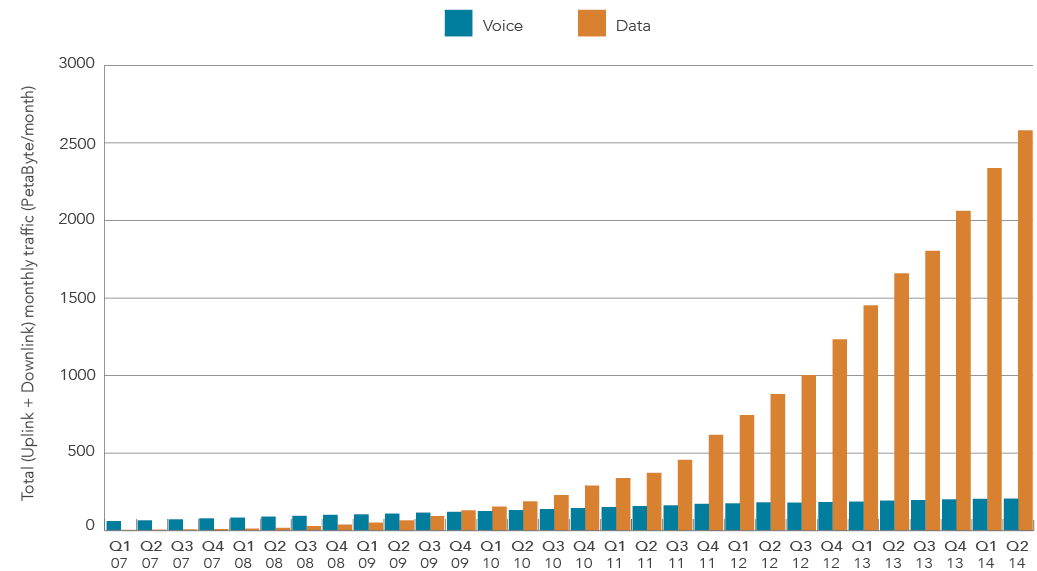
\includegraphics[scale=0.5]{imagenes/conexiones_moviles}
	\caption{Registros de la compañía \emph{Ericsson} ilustrando el crecimiento exponencial en el uso de datos de los dispositivos móviles. Parte del informe de \emph{Akamai} \cite{report:akamai}}
	\label{fig:akamai_stats}
\end{figure}

Más allá del número de dispositivos o la cantidad --o calidad-- del acceso a Internet, las distintas aplicaciones actuales han evolucionado sobre la base de protocolos y sistemas diseñados hace varias décadas, pero exigiendo siempre la mejor performance posible en pos de garantizar buenos tiempos de respuesta. Los protocolos más celebres de la llamada \emph{familia de protocolos de Internet} son TCP e IP. Sin embargo, son decenas los protocolos y mecanismos involucrados en las diferentes fases de comunicación entre computadoras y aplicaciones, que permiten en conjunto la operación de la red de redes como hoy la conocemos.

\section*{El modelo OSI}
La capacidad de conectividad entre 2 distintos dispositivos es resultado del efecto combinado de varias capas de abstracción con responsabilidades divididas. Un diseño de operación que se ilustra en un modelo estándar vigente desde los años 80 es el impulsado por la \emph{Organización Internacional de Normalización} (ISO), mejor conocido como el modelo \textbf{OSI}\footnote{Por sus siglas en inglés \emph{Open System Interconnection}.}. En la práctica, la importancia de éste modelo radica en servir como una referencia técnica que ilustra los límites en las responsabilidades entre componentes que conforman una arquitectura de interconexión de sistemas.

El modelo OSI reconoce 7 capas de abstracción en el proceso de comunicación entre dispositivos (Ver figura \ref{fig:osi7capas}), cada una con obligaciones específicas, pero que combinadas soportan constructivamente un mecanismo de comunicación estándar para sistemas que por él se rijan. El acierto de éste enfoque está en permitir el desarrollo de soluciones modulares y especificas a cada una de las capas, sin interferir entre capas diferentes y manteniendo así la compatibilidad con aplicaciones que ya operen en capas distintas. Las 7 capas en cuestión se describen a continuación:

\begin{figure}[!h]
	\centering
	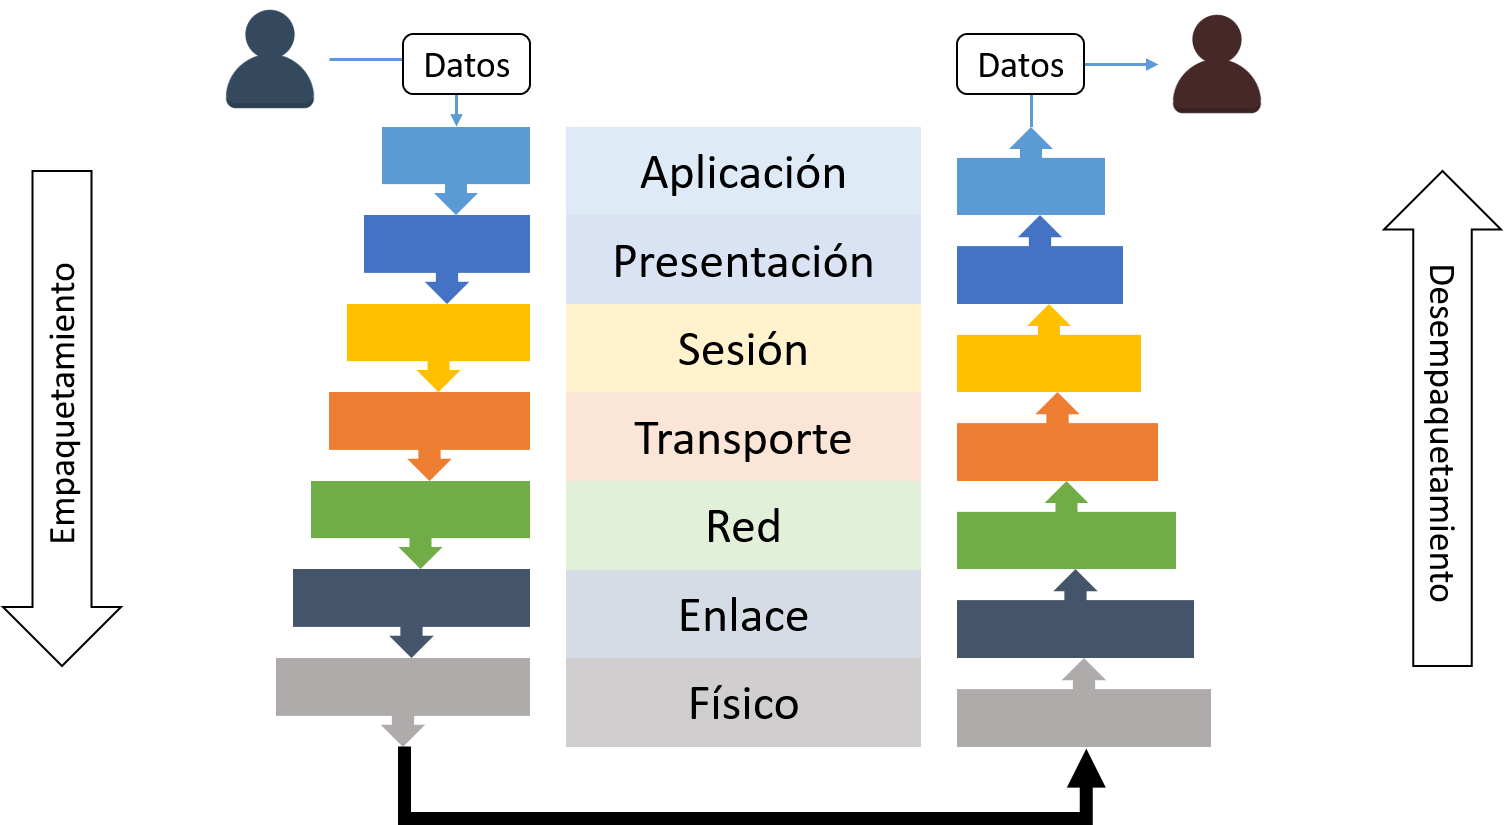
\includegraphics[scale=.45]{imagenes/OSI7Capas.png}
	\caption{Diagrama esquemático de las 7 capas del modelo OSI, ilustrando el proceso de encapsulamiento y desencapsulamiento de datos al ir agregando y removiendo encabezados de capa, según los procesos de empaquetamiento y desempaquetamiento, respectivamente.}
	\label{fig:osi7capas}
\end{figure}

\begin{description}
\item[Capa Física] La capa de nivel inferior en el modelo OSI es la capa física. Es ésta capa la responsible de la topología de la red y de la especificación de los medios materiales que consiguen la transmisión de la información, así como también es responsable de la generación real de la comunicación por medio del envío de la información. Es, en definitiva, la encargada del paso a canales físicos de la información a transmitir.

\item[Capa de Enlace] Es la segunda capa del modelo. Ella se encarga de proveer un mecanismo de direccionamiento físico en una máquina que permita el reconocimiento individual de la misma, proveiendo de un primer identificador a las máquinas en el modelo OSI dado por las direcciones físicas de los dispositivos (\emph{MAC}). Es responsable también de proveer mecanismos de corrección de errores en el proceso de transmisión de datos que pudiesen manifestarse por problemas de la capa física, haciendo dicha comunicación, desde éste punto, confiable.

\item[Capa de Red] Es la tercera capa del modelo OSI. Hace su debut en contextos de multiples equipos interconectados brindando mecanismos de identificación para proveer una capacidad de direccionamiento más amplia con respecto al disponible en las dos primeras capas (que sólo permitian la comunicación entre un par de máquinas, punto a punto). En éste nivel aparece uno de los protocolos más populares en Internet, el denominado protocolo IP que supone un mecanismo de identificación único para cada dispositivo en una red, provisto en base a una dirección homónima. Ésta capa establece la capacidad de ruteo en la comunicación como una responsabilidad de los nodos en una infraestructura en red, haciendo cada componente de la red alcanzable para cualquier otro integrante de la misma.

\item[Capa de Transporte] La cuarta capa del modelo, es la que provee de lleno la capacidad de transporte de datos. En éste nivel se incorporan los también celebres protocolos homónimos: TCP (orientado a la conexión) y UDP (orientado a la mensajería). Ésta capa es también responsible de brindar la capacidad de multiplexación a nivel de una máquina, permitiendo la generación de multiples conexiones desde el mismo dispositivo. Dicho mecanismo lo consigue al incorporar puertos numerados, que sirven como puntos lógicos de comunicación. De ésta manera, a partir de la capa de transporte se establece un paradigma base en el área de redes, en lo que a programación y esquematización de la misma corresponde: La construcción de conexiones \emph{IP:PUERTO}, que son la base del concepto de tuplas de direccionamiento en el proceso de transporte de datos.

\item[Capa de Sesión] Es la quinta capa del modelo OSI. Tal y como su nombre lo indica su función radica en ser la responsible de mantener un control de sesión en una conexión entre extremos, proveiendo mecanismos de corrección y reconexion en caso de interferencia de una operación entre máquinas. Es responsable de mantener el enlace de comunicación construido en base a las capas inferiores en un proceso de comunicación.

\item[Capa de Presentación] El sexto nivel en el modelo OSI es la capa de presentación, cuya responsabilidad comprende proveer el soporte para dar una correcta interpretación de los datos transmitidos, de manera de conseguir que los datos lleguen de manera reconocible al host de destino. A diferencia de las capas inferiores que se enfocan en los mecanismos de envío de la infromación, ésta capa guarda directa relación con la información transmitida y con su correcta interpretación final.

\item[Capa de Aplicación] Es la última -y de más alto nivel- capa de abstracción del modelo OSI. Es la responsible de proveer una interfaz simple a aplicaciones al acceso a mecanismos de comunicación en red. En otras palabras, es la responsible de proveer el servicio de comunicaciones a las distintas aplicaciones que tengan distintos requerimientos de comunicación.

\end{description}

A pesar de que el modelo OSI plantea responsabilidades delimitadas a cada capa de abstracción, la correspondencia de dicho estándar teórico en la práctica es una labor que queda supeditada a los programadores de sistemas operativos. Finalmente son ellos los que, en mayor o menor medida, hacen corresponder para con el modelo las implementaciones finales de los módulos de red de un sistema.


\section*{Familia de Protocolos de Internet}
El conjunto de múltiples protocolos que facultan a los sistemas con mecanismos de interconexión comprende a varios cientos que se distribuyen entre las distintas capas del modelo OSI. A este conjunto se le denomina \emph{Familia de Protocolos de Internet}. Sin embargo, históricamente se le ha prestado especial atención a un subconjunto de ellos que son estructurales en la infraestructura predominante de Internet y que rigen la misma, hablamos del conjunto de protocolos \textbf{TCP/IP}.

La arquitectura de los protocolos TCP/IP sigue la inspiración del modelo OSI en las responsabilidades a soportar --a pesar de romper la estructura de capas del mismo-- combinando algunas responsabilidades de dicho modelo en funciones únicas y obviando otras. Un ejemplo de esto se puede apreciar en la tabla \ref{tabla:tcpiposi} que ilustra la correspondencia de los protocolos del conjunto TCP/IP con su atribución según el modelo OSI.

\begin{table}[h!]
\centering
\begin{tabular}{|c|p{4cm}|l|p{5cm}|}
\hline
\multicolumn{1}{|c|}{\textbf{\begin{tabular}[c]{@{}c@{}}Ref. OSI\\ Nº de capa\end{tabular}}} & \multicolumn{1}{c|}{\textbf{\begin{tabular}[c]{@{}c@{}}Equivalente \\ de capa OSI\end{tabular}}} & \multicolumn{1}{c|}{\textbf{Capa TCP/IP}} & \multicolumn{1}{c|}{\textbf{\begin{tabular}[c]{@{}c@{}}Ejemplos de\\ protocolos TCP/IP\end{tabular}}} \\ \hline
5,6,7                                                                                        & Aplicación, Sesión, Presentación                                                                 & Aplicación                                & NFS, NIS, DNS, LDAP, telnet, ftp, rlogin, rsh, rcp, RIP, RDISC, SNMP y otros.                         \\ \hline
4                                                                                            & Transporte                                                                                       & Transporte                                & TCP, UDP, SCTP                                                                                        \\ \hline
3                                                                                            & Red                                                                                              & Internet                                  & IPv4, IPv6, ARP, ICMP                                                                                 \\ \hline
2                                                                                            & Vínculo de datos                                                                                 & Vínculo de datos                          & PPP, IEEE 802.2                                                                                       \\ \hline
1                                                                                            & Física                                                                                           & Red física                                & Ethernet (IEEE 802.3), Token Ring, RS-232, FDDI y otros.                                              \\ \hline
\end{tabular}
\caption{Comparativa de correspondencia de algunos protocolos de la familia de Internet de acuerdo al modelo OSI.}
\label{tabla:tcpiposi}
\end{table}
%\url{https://docs.oracle.com/cd/E19957-01/820-2981/6nei0r0r9/index.html}

\subsection*{UDP}
UDP \cite{rfc:768} es un protocolo de la familia de protocolos de Internet con funciones a nivel de la capa de transporte según el modelo OSI, que se caracteriza por ser un protocolo orientado a mensajes, vale decir, por permitir enviar mensajes a través de la red sin necesidad de establecer previamente una conexión con el equipo receptor (situación que si ocurre y es característica de los protocolos orientados a la conexión como es el caso de TCP).
%[OSI reference model—The ISO model of architecture for open systems interconnection]%

Ésta naturaleza de UDP tiene varias implicancias:
\begin{itemize}
\item En primer lugar, ser un protocolo orientado a mensajes supone una premura en el envío de información, ello significa que éste protocolo no verifica la correctitud en la recepción de los datos enviados. En ese sentido, UDP es lo que se denomina un protocolo \textbf{no fiable}.
\item Por otro lado, UDP trabaja en estados denominados \textbf{sin conexión}, lo que significa que no hay una verdadera sincronización entre origen y destino. Esto supone el uso de operaciones del tipo asíncronas las que hacen más flexible la comunicación entre los extremos.
\end{itemize}

Por su funcionamiento, la anatomía o estructura de un paquete UDP es bastante simple (Ver fig. \ref{fig:datagramaudp}). Al ser un protocolo orientado al envío de mensajes, los paquetes disponen de pocos campos de información, de manera de evitar sobrecargar los mismos en su transferencia. Así mismo, en éste nivel los paquetes se denominan \emph{datagramas}. Los encabezados de un paquete UDP comprenden: \textbf{Puerto de Origen/Destino}, que hace referencia a los puntos de conexión de la capa Transporte del modelo OSI y \textbf{Longitud del Mensaje} y \textbf{\emph{Checksum}}\footnote{Corresponde a un valor generado a partir de una función matemática que se aplica sobre datos para corroborar la integridad de los mismos y su correcta recepción tras un envío.}, que sirven como componentes de verificación del paquete mismo.

\begin{figure}[!h]
	\centering
	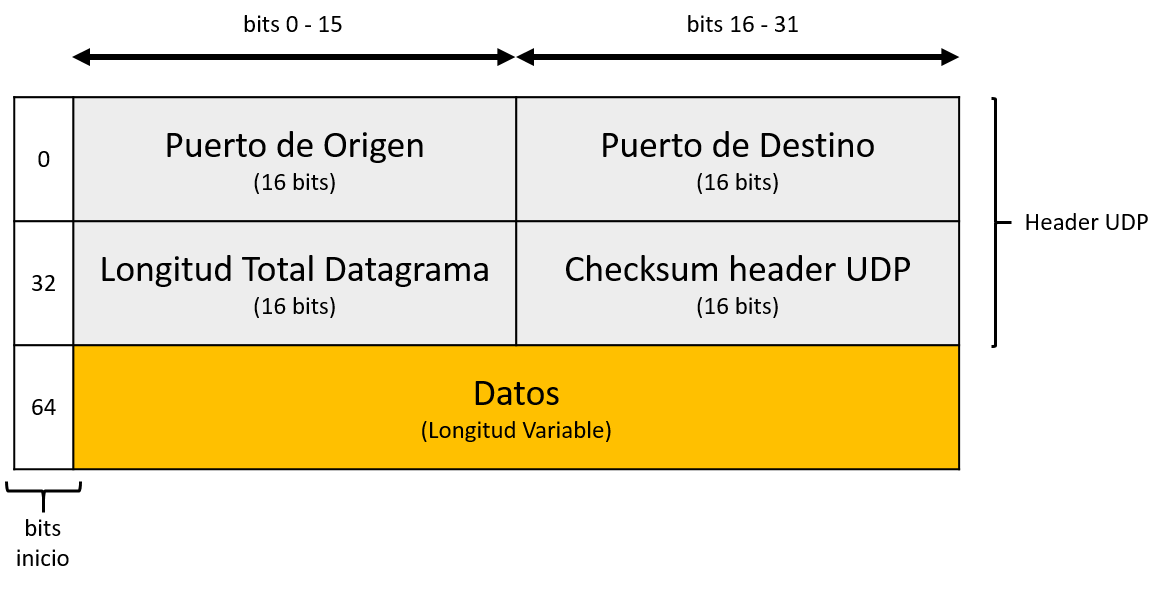
\includegraphics[scale=.55]{imagenes/estructuraUDP.png}
	\caption{Estructura de un paquete UDP con detalle del tamaño de sus encabezados de capa de transporte.}
	\label{fig:datagramaudp}
\end{figure}

El protocolo UDP se estandarizó el año 1980, sin embargo su aplicación ha sido muy variada en distintos sistemas modernos. Hoy por hoy UDP es uno de los componentes estructurales de la Internet estando presente en diversas aplicaciones que van desde transmisiones en uso intensivo de datos para redes de alta velocidad \cite{udp:highbandwidth}, hasta mecanismos de transmisión de video \cite{udp:video}, entre otros. Sin embargo, una de las aplicaciones más importantes (sino la más trascendental) de éste protocolo en la infraestructura de Internet, es su labor en el servicio DNS.

\subsection*{DNS}
\label{section:dns}
Todo dispositivo conectado a una red de computadoras se identifica a si mismo por la denominada \emph{dirección IP}, un identificador que permite referenciarlo y diferenciarlo de otros dispositivos conectados a la misma red, definido por el nivel 3 del modelo OSI. No obstante para poder conectarse con un recurso disponible en Internet, generalmente los dispositivos consultan por lo que llamamos \emph{nombres de dominio}, que son identificadores con carácter semántico para los usuarios que definen una red de identificación asociada a un grupo de dispositivos o equipos conectados a la red \cite{wiki:nombre_dominio}. Éste mecanismo de traducciones se conoce como \textbf{servicio DNS} y es vital para el funcionamiento de Internet como lo conocemos.

El servicio DNS \cite{rfc:1034, rfc:1035} opera como una base de datos distribuida que permite resolver consultas de manera jerarquizada basado en un principio de consultas recursivas. Frente a una consulta por un nombre de dominio, el primer paso es la resolución de la misma empleando datos de la caché local del servicio DNS del sistema (Esto es, emplear información previa en caso de que el nombre consultado ya hubiese sido preguntado anteriormente). En caso de encontrarse la respuesta en la caché local, se responde la consulta con ésta información y el proceso finaliza. En caso de que la consulta no coincida con algún registro local, se promueve el proceso de resolución de nombre al servidor DNS preferido (Configurado en el sistema).  

Frente a una consulta, un servidor DNS hace una verificación en su información local para determinar si tiene autoridad para responder al nombre solicitado en función de la zona que tenga configurada. En caso de que el nombre consultado coincida con algún registro de dicho servidor, el servidor usa ésta información para responder la consulta con autoridad y finaliza el proceso. En caso de que éste servidor no disponga de una entrada con el nombre pedido, se verifica en su caché local en caso de que previamente el servidor hubiese formado parte de una cadena de resolución para el nombre pedido, en cuyo caso puede responder con la resolución almacenada en caché y finalizar la consulta. Si tras todas las verificaciones anteriores (Sobre los registros de la zona DNS y de caché de resoluciones) el nombre de dominio consultado no registra apariciones en el servidor DNS preferido, la consulta se promueve recursivamente a otros servidores DNS con sugerencias de raíz para el nombre solicitado, de manera de poder conseguir una respuesta autoritativa en cada caso. Para esto la consulta se resuelve desde el dominio de nivel superior, resolviendo desde lo general a lo particular del nombre de dominio. Un ejemplo de resolución del dominio dcc.uchile.cl se ilustra en la imagen \ref{fig:dns}

\begin{figure}[!h]
	\centering
	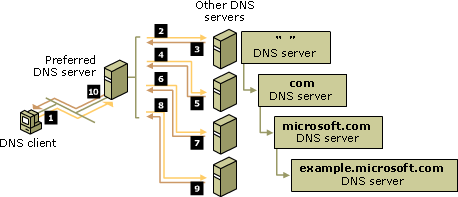
\includegraphics[scale=0.75]{imagenes/dns-system.png}
	\caption{Diagrama de operación del servicio DNS ilustrando comunicación entre servidores de dicho tipo.}
	\label{fig:dns}
\end{figure}

En la práctica, el servicio DNS emplea el protocolo UDP para la comunicación desde y hacia los servidores de dicho tipo, esto pues las características de una consulta DNS contemplan:

\begin{itemize}
\item \textbf{Consultas Auto-Contenidas} La información de una consulta DNS calza fácilmente en un paquete de UDP.
\item \textbf{Orden Irrelevante} Los requerimientos DNS no necesitan ser procesados en un orden establecido. Sin embargo, si requieren ser eventualmente procesados y ello en el menor tiempo posible. Un factor que justifica el uso de UDP al ser precisamente un protocolo orientado a mensajes.
\end{itemize}

De esta manera, las características anteriores justifican el uso de UDP como protocolo para la comunicación entre los servidores DNS.

El escenario antes descrito explica el por qué UDP tiene una participación de gran importancia en las redes actuales (en especial sobre Internet) y además, dado el sostenido aumento en el número de conexiones explicado en las secciones previas, da cuenta de cómo el tráfico de éste tipo de comunicación representa una porción muy significativa en la operación de las redes modernas. Una situación que con el paso de los años ha exigido cada vez mejores técnicas de procesamiento para dar mejores tiempos de respuesta.

\section*{Planteamineto de Investigación}

La pregunta natural entonces es: ¿Están capacitados los servidores DNS para responder tal cantidad de peticiones correctamente? Más allá de la respuesta a ésta interrogante el hecho es que, para su correcta operación, los servidores DNS deben garantizar bajos tiempos de respuesta y eficiencia en su operación en todo escenario.

Un excelente enfoque para abordar la problemática anterior mora en usar paralelismo, ósea, aprovechar la independencia entre peticiones DNS para procesar varios requerimientos a la vez de manera simultánea. En la práctica, dicha solución propone compartir una misma interfaz de conexión (denominada \emph{Socket}) entre varios hilos de ejecución. Ésta práctica supone --en teoría-- un incremento en el rendimiento de operación del procesamiento de las peticiones DNS, siempre que existan procesadores disponibles para atender cada hilo de forma independiente.

Sin embargo, los resultados al evaluar el enfoque antes propuesto revelan un preocupante e insospechado panorama donde el rendimiento de los servidores DNS no escala al incorporar directamente paralelismo en el procesamiento de peticiones como se esperaría \cite{tesis:diegoDCC}. Éste fenómeno ha sido repasado por distintos grupos de investigación en el área como Facebook, Toshiba \cite{post:facebook, paper:toshiba} e incluso industrias nacionales como NIC Chile, pero sin mayor solución más que delegar dicha responsabilidad a unidades estructurales del sistema operativo (como el kernel del sistema operativo) de donde tampoco se han conseguido mayores mejoras.

La pregunta entonces es ¿Por qué el sistema de procesamiento de peticiones DNS no escala al incorporar paralelismo directamente? Una sospecha interesante propone que probablemente el sistema de procesamiento de paquetes para UDP (que es el protocolo involucrado en las peticiones DNS) podría tener imperfecciones a nivel de diseño en el sistema operativo que no garantizarían su óptimo funcionamiento en condiciones de concurrencia, sugiriendo como responsable del problema a un defecto de contención a nivel de estructuras compartidas del sistema operativo. Sin embargo, dicha hipótesis no ha sido comprobada ni desmentida. Por otra parte, determinar la causa del problema anterior significa un tremendo desafío pues implica trabajar a nivel del núcleo del sistema operativo, que combina diversos paradigmas y enfoques de programación incorporados a lo largo de su desarrollo, unido a la dificultad inherente de trabajar analizando un sistema complejo como lo es el kernel mismo.

El presente trabajo plantea precisamente un estudio amplio que reune las principales sospechas de investigación vigentes del problema al momento de su desarrollo, de manera de identificar y analizar las distintas componentes responsables del problema detectado, así como también el estudio de alternativas para palear dicha situación.


\end{intro}
\begin{intro}
Desde sus orígenes, nunca se sospechó el grado de penetración y protagonismo que llegaría a alcanzar Internet. De acuerdo a importantes y periódicos estudios sobre dicha red \cite{report:akamai} la tónica de últimos años se podría caracterizar como: Grandes y sostenidos incrementos tanto en el número de conexiones a Internet como en la velocidad de las mismas. Éste factor de alto crecimiento es seguramente la característica fundamental de la llamada ``Era de la información'' que nos ha repletado de dispositivos demandando constantemente acceso a Internet. Un escenario que postula todo un desafío para la infraestructura --tanto de hardware como de software-- disponible de la red.

\section*{Crecimiento de la red}
El gran crecimiento en la cantidad de sistemas tecnológicos interconectados vía Internet en el mundo en los últimos 30 años es algo que no ha dejado indiferente a nadie\footnote{\url{http://www.internetworldstats.com/emarketing.htm}}. Para entender este fenómeno distintos organismos internacionales se dedican periódicamente a realizar estimaciones de dicha cifra. Un caso muy popular de esta labor es el contador global de conexiones móviles a Internet del \emph{GSMA Intelligence}\footnote{\url{https://gsmaintelligence.com/}} el cual recientemente ha estimado en más de 7 mil millones el número de dispositivos móviles con conexión a la red, superando por primera vez al total de la población mundial\footnote{\url{http://www.cnet.com/news/there-are-now-more-gadgets-on-earth-than-people/}}. Una premisa que coincide con el último informe \emph{The State Of Internet} de la corporación \emph{Akamai} \cite{report:akamai} donde se resume el estudio de las principales variaciones en capacidad de acceso, velocidades de acceso, tipos de ataques, etc. a Internet de que disponen distintos países del mundo. Éste estudio corroboró lo que ya ha sido tendencia en los últimos años: Tanto las velocidades de navegación, como el total de conexiones a Internet han aumentado generalizadamente en todo el planeta (Ver figura \ref{fig:akamai_stats}). Las proyecciones a futuro preservan ésta tendencia apostando a que tanto la cantidad de dispositivos como el número de accesos a Internet deberían seguir subiendo \cite{nota:2020}, ello producto de factores como la reducción de costos de producción y la minimización de la tecnología, además de distintas tendencias generadas a raíz del fenómeno de \emph{globalización} que --en gran medida-- nos ha forzado a participar de una sociedad más interconectada en todo el mundo. Olvidando un poco las interpretaciones o justificaciones para ésta situación, el hecho concreto es que existe una directa proporcionalidad entre el número de dispositivos y los requerimientos de accesos a la red, y hoy ambos están en su apogeo de crecimiento.

\begin{figure}[!h]
	\centering
	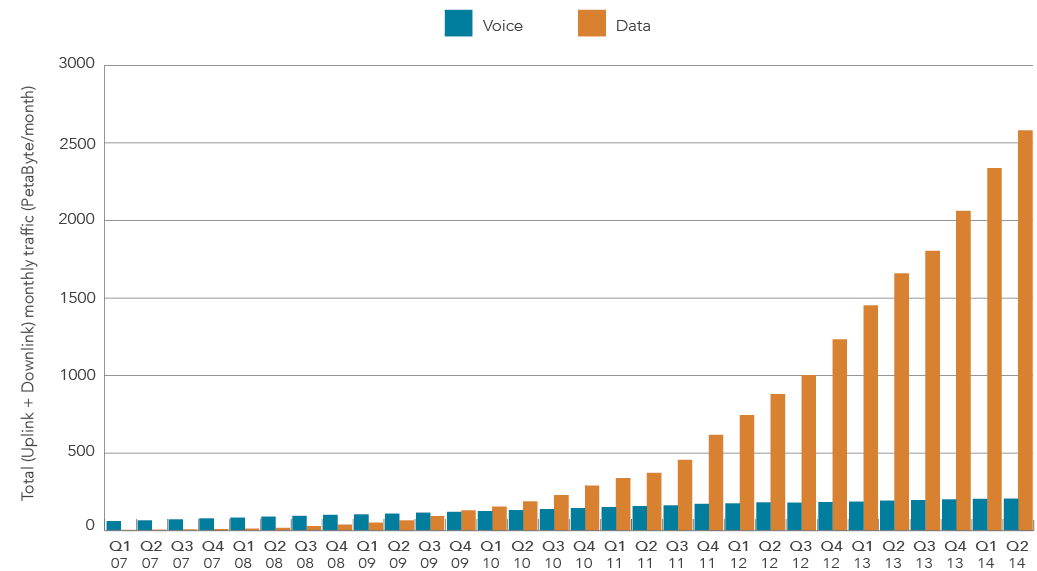
\includegraphics[scale=0.5]{imagenes/conexiones_moviles}
	\caption{Registros de la compañía \emph{Ericsson} ilustrando el crecimiento exponencial en el uso de datos de los dispositivos móviles. Parte del informe de \emph{Akamai} \cite{report:akamai}}
	\label{fig:akamai_stats}
\end{figure}

Más allá del número de dispositivos o la cantidad --o calidad-- del acceso a Internet, las distintas aplicaciones actuales han evolucionado sobre la base de protocolos y sistemas diseñados hace varias décadas, pero exigiendo siempre la mejor performance posible en pos de garantizar buenos tiempos de respuesta. Los protocolos más celebres de la llamada \emph{familia de protocolos de Internet} son TCP e IP. Sin embargo, son decenas los protocolos y mecanismos involucrados en las diferentes fases de comunicación entre computadoras y aplicaciones, que permiten en conjunto la operación de la red de redes como hoy la conocemos.

\section*{El modelo OSI}
La capacidad de conectividad entre 2 distintos dispositivos es resultado del efecto combinado de varias capas de abstracción con responsabilidades divididas. Un diseño de operación que se ilustra en un modelo estándar vigente desde los años 80 es el impulsado por la \emph{Organización Internacional de Normalización} (ISO), mejor conocido como el modelo \textbf{OSI}\footnote{Por sus siglas en inglés \emph{Open System Interconnection}.}. En la práctica, la importancia de éste modelo radica en servir como una referencia técnica que ilustra los límites en las responsabilidades entre componentes que conforman una arquitectura de interconexión de sistemas.

El modelo OSI reconoce 7 capas de abstracción en el proceso de comunicación entre dispositivos (Ver figura \ref{fig:osi7capas}), cada una con obligaciones específicas, pero que combinadas soportan constructivamente un mecanismo de comunicación estándar para sistemas que por él se rijan. El acierto de éste enfoque está en permitir el desarrollo de soluciones modulares y especificas a cada una de las capas, sin interferir entre capas diferentes y manteniendo así la compatibilidad con aplicaciones que ya operen en capas distintas. Las 7 capas en cuestión se describen a continuación:

\begin{figure}[!h]
	\centering
	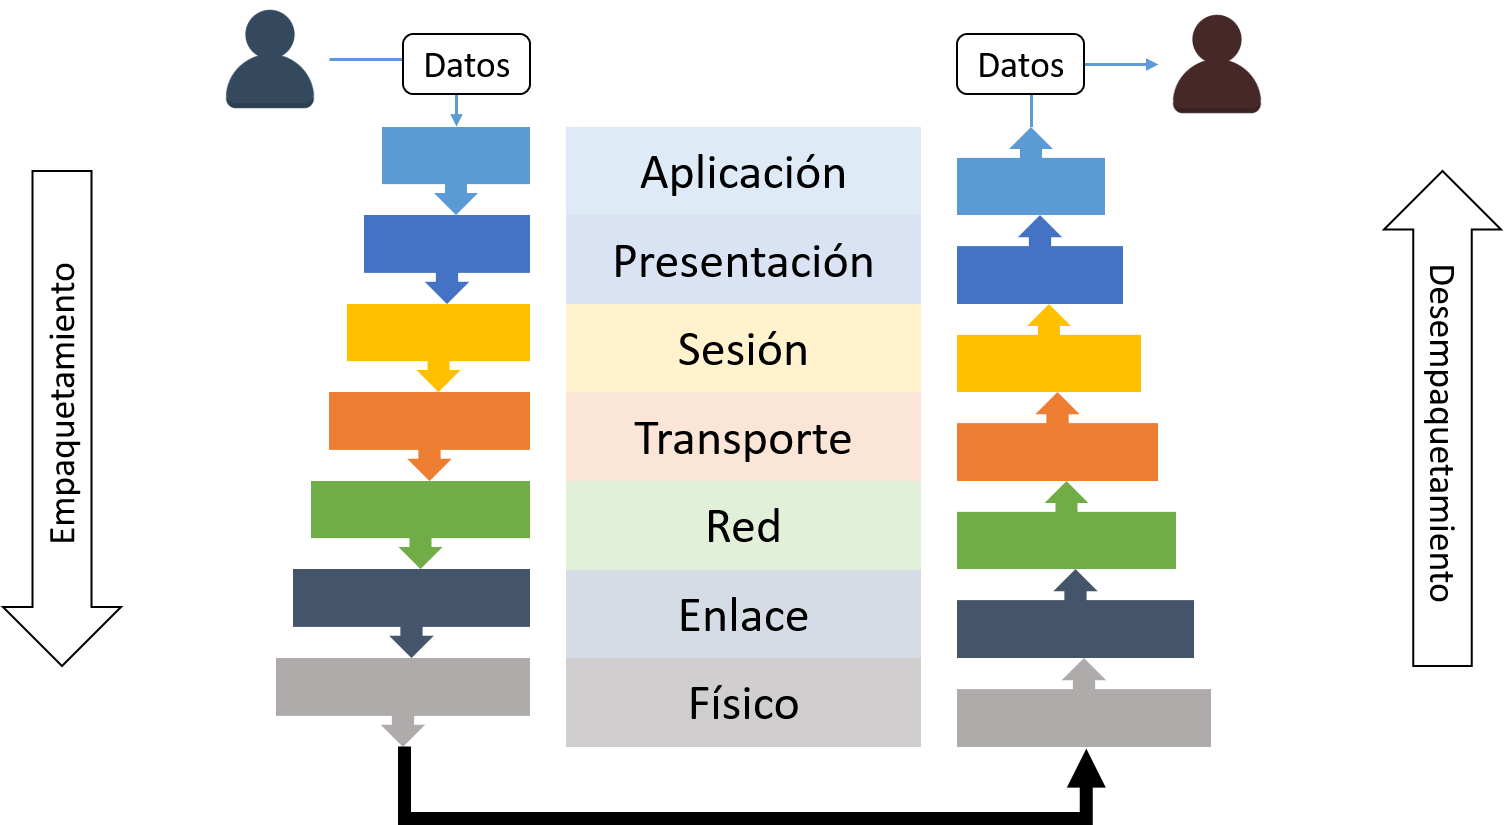
\includegraphics[scale=.45]{imagenes/OSI7Capas.png}
	\caption{Diagrama esquemático de las 7 capas del modelo OSI, ilustrando el proceso de encapsulamiento y desencapsulamiento de datos al ir agregando y removiendo encabezados de capa, según los procesos de empaquetamiento y desempaquetamiento, respectivamente.}
	\label{fig:osi7capas}
\end{figure}

\begin{description}
\item[Capa Física] La capa de nivel inferior en el modelo OSI es la capa física. Es ésta capa la responsible de la topología de la red y de la especificación de los medios materiales que consiguen la transmisión de la información, así como también es responsable de la generación real de la comunicación por medio del envío de la información. Es, en definitiva, la encargada del paso a canales físicos de la información a transmitir.

\item[Capa de Enlace] Es la segunda capa del modelo. Ella se encarga de proveer un mecanismo de direccionamiento físico en una máquina que permita el reconocimiento individual de la misma, proveiendo de un primer identificador a las máquinas en el modelo OSI dado por las direcciones físicas de los dispositivos (\emph{MAC}). Es responsable también de proveer mecanismos de corrección de errores en el proceso de transmisión de datos que pudiesen manifestarse por problemas de la capa física, haciendo dicha comunicación, desde éste punto, confiable.

\item[Capa de Red] Es la tercera capa del modelo OSI. Hace su debut en contextos de multiples equipos interconectados brindando mecanismos de identificación para proveer una capacidad de direccionamiento más amplia con respecto al disponible en las dos primeras capas (que sólo permitian la comunicación entre un par de máquinas, punto a punto). En éste nivel aparece uno de los protocolos más populares en Internet, el denominado protocolo IP que supone un mecanismo de identificación único para cada dispositivo en una red, provisto en base a una dirección homónima. Ésta capa establece la capacidad de ruteo en la comunicación como una responsabilidad de los nodos en una infraestructura en red, haciendo cada componente de la red alcanzable para cualquier otro integrante de la misma.

\item[Capa de Transporte] La cuarta capa del modelo, es la que provee de lleno la capacidad de transporte de datos. En éste nivel se incorporan los también celebres protocolos homónimos: TCP (orientado a la conexión) y UDP (orientado a la mensajería). Ésta capa es también responsible de brindar la capacidad de multiplexación a nivel de una máquina, permitiendo la generación de multiples conexiones desde el mismo dispositivo. Dicho mecanismo lo consigue al incorporar puertos numerados, que sirven como puntos lógicos de comunicación. De ésta manera, a partir de la capa de transporte se establece un paradigma base en el área de redes, en lo que a programación y esquematización de la misma corresponde: La construcción de conexiones \emph{IP:PUERTO}, que son la base del concepto de tuplas de direccionamiento en el proceso de transporte de datos.

\item[Capa de Sesión] Es la quinta capa del modelo OSI. Tal y como su nombre lo indica su función radica en ser la responsible de mantener un control de sesión en una conexión entre extremos, proveiendo mecanismos de corrección y reconexion en caso de interferencia de una operación entre máquinas. Es responsable de mantener el enlace de comunicación construido en base a las capas inferiores en un proceso de comunicación.

\item[Capa de Presentación] El sexto nivel en el modelo OSI es la capa de presentación, cuya responsabilidad comprende proveer el soporte para dar una correcta interpretación de los datos transmitidos, de manera de conseguir que los datos lleguen de manera reconocible al host de destino. A diferencia de las capas inferiores que se enfocan en los mecanismos de envío de la infromación, ésta capa guarda directa relación con la información transmitida y con su correcta interpretación final.

\item[Capa de Aplicación] Es la última -y de más alto nivel- capa de abstracción del modelo OSI. Es la responsible de proveer una interfaz simple a aplicaciones al acceso a mecanismos de comunicación en red. En otras palabras, es la responsible de proveer el servicio de comunicaciones a las distintas aplicaciones que tengan distintos requerimientos de comunicación.

\end{description}

A pesar de que el modelo OSI plantea responsabilidades delimitadas a cada capa de abstracción, la correspondencia de dicho estándar teórico en la práctica es una labor que queda supeditada a los programadores de sistemas operativos. Finalmente son ellos los que, en mayor o menor medida, hacen corresponder para con el modelo las implementaciones finales de los módulos de red de un sistema.


\section*{Familia de Protocolos de Internet}
El conjunto de múltiples protocolos que facultan a los sistemas con mecanismos de interconexión comprende a varios cientos que se distribuyen entre las distintas capas del modelo OSI. A este conjunto se le denomina \emph{Familia de Protocolos de Internet}. Sin embargo, históricamente se le ha prestado especial atención a un subconjunto de ellos que son estructurales en la infraestructura predominante de Internet y que rigen la misma, hablamos del conjunto de protocolos \textbf{TCP/IP}.

La arquitectura de los protocolos TCP/IP sigue la inspiración del modelo OSI en las responsabilidades a soportar --a pesar de romper la estructura de capas del mismo-- combinando algunas responsabilidades de dicho modelo en funciones únicas y obviando otras. Un ejemplo de esto se puede apreciar en la tabla \ref{tabla:tcpiposi} que ilustra la correspondencia de los protocolos del conjunto TCP/IP con su atribución según el modelo OSI.

\begin{table}[h!]
\centering
\begin{tabular}{|c|p{4cm}|l|p{5cm}|}
\hline
\multicolumn{1}{|c|}{\textbf{\begin{tabular}[c]{@{}c@{}}Ref. OSI\\ Nº de capa\end{tabular}}} & \multicolumn{1}{c|}{\textbf{\begin{tabular}[c]{@{}c@{}}Equivalente \\ de capa OSI\end{tabular}}} & \multicolumn{1}{c|}{\textbf{Capa TCP/IP}} & \multicolumn{1}{c|}{\textbf{\begin{tabular}[c]{@{}c@{}}Ejemplos de\\ protocolos TCP/IP\end{tabular}}} \\ \hline
5,6,7                                                                                        & Aplicación, Sesión, Presentación                                                                 & Aplicación                                & NFS, NIS, DNS, LDAP, telnet, ftp, rlogin, rsh, rcp, RIP, RDISC, SNMP y otros.                         \\ \hline
4                                                                                            & Transporte                                                                                       & Transporte                                & TCP, UDP, SCTP                                                                                        \\ \hline
3                                                                                            & Red                                                                                              & Internet                                  & IPv4, IPv6, ARP, ICMP                                                                                 \\ \hline
2                                                                                            & Vínculo de datos                                                                                 & Vínculo de datos                          & PPP, IEEE 802.2                                                                                       \\ \hline
1                                                                                            & Física                                                                                           & Red física                                & Ethernet (IEEE 802.3), Token Ring, RS-232, FDDI y otros.                                              \\ \hline
\end{tabular}
\caption{Comparativa de correspondencia de algunos protocolos de la familia de Internet de acuerdo al modelo OSI.}
\label{tabla:tcpiposi}
\end{table}
%\url{https://docs.oracle.com/cd/E19957-01/820-2981/6nei0r0r9/index.html}

\subsection*{UDP}
UDP \cite{rfc:768} es un protocolo de la familia de protocolos de Internet con funciones a nivel de la capa de transporte según el modelo OSI, que se caracteriza por ser un protocolo orientado a mensajes, vale decir, por permitir enviar mensajes a través de la red sin necesidad de establecer previamente una conexión con el equipo receptor (situación que si ocurre y es característica de los protocolos orientados a la conexión como es el caso de TCP).
%[OSI reference model—The ISO model of architecture for open systems interconnection]%

Ésta naturaleza de UDP tiene varias implicancias:
\begin{itemize}
\item En primer lugar, ser un protocolo orientado a mensajes supone una premura en el envío de información, ello significa que éste protocolo no verifica la correctitud en la recepción de los datos enviados. En ese sentido, UDP es lo que se denomina un protocolo \textbf{no fiable}.
\item Por otro lado, UDP trabaja en estados denominados \textbf{sin conexión}, lo que significa que no hay una verdadera sincronización entre origen y destino. Esto supone el uso de operaciones del tipo asíncronas las que hacen más flexible la comunicación entre los extremos.
\end{itemize}

Por su funcionamiento, la anatomía o estructura de un paquete UDP es bastante simple (Ver fig. \ref{fig:datagramaudp}). Al ser un protocolo orientado al envío de mensajes, los paquetes disponen de pocos campos de información, de manera de evitar sobrecargar los mismos en su transferencia. Así mismo, en éste nivel los paquetes se denominan \emph{datagramas}. Los encabezados de un paquete UDP comprenden: \textbf{Puerto de Origen/Destino}, que hace referencia a los puntos de conexión de la capa Transporte del modelo OSI y \textbf{Longitud del Mensaje} y \textbf{\emph{Checksum}}\footnote{Corresponde a un valor generado a partir de una función matemática que se aplica sobre datos para corroborar la integridad de los mismos y su correcta recepción tras un envío.}, que sirven como componentes de verificación del paquete mismo.

\begin{figure}[!h]
	\centering
	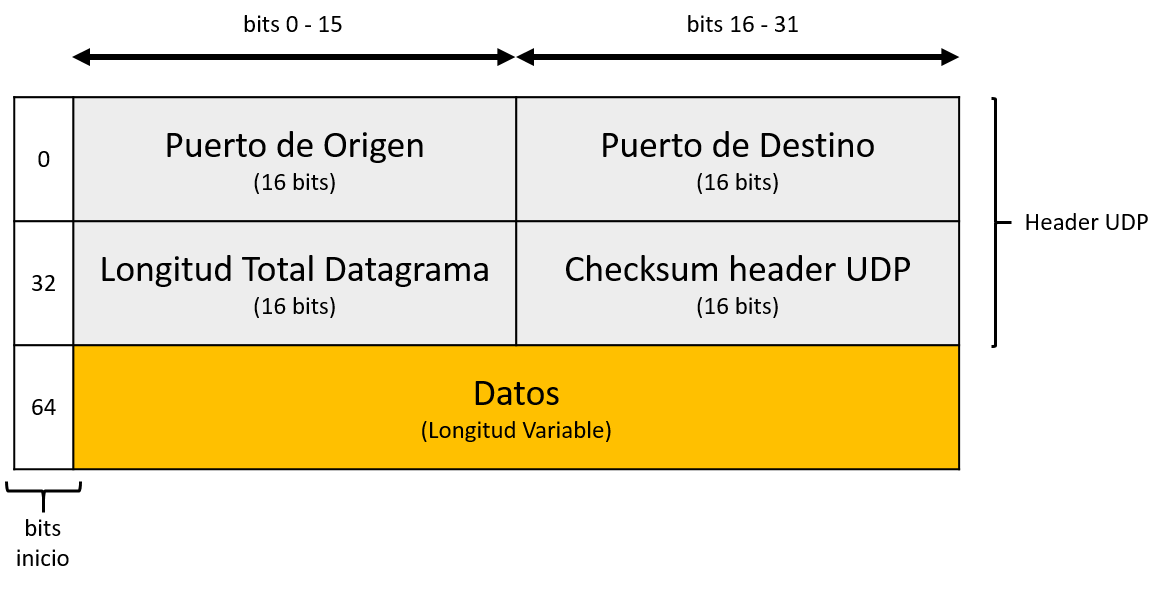
\includegraphics[scale=.55]{imagenes/estructuraUDP.png}
	\caption{Estructura de un paquete UDP con detalle del tamaño de sus encabezados de capa de transporte.}
	\label{fig:datagramaudp}
\end{figure}

El protocolo UDP se estandarizó el año 1980, sin embargo su aplicación ha sido muy variada en distintos sistemas modernos. Hoy por hoy UDP es uno de los componentes estructurales de la Internet estando presente en diversas aplicaciones que van desde transmisiones en uso intensivo de datos para redes de alta velocidad \cite{udp:highbandwidth}, hasta mecanismos de transmisión de video \cite{udp:video}, entre otros. Sin embargo, una de las aplicaciones más importantes (sino la más trascendental) de éste protocolo en la infraestructura de Internet, es su labor en el servicio DNS.

\subsection*{DNS}
\label{section:dns}
Todo dispositivo conectado a una red de computadoras se identifica a si mismo por la denominada \emph{dirección IP}, un identificador que permite referenciarlo y diferenciarlo de otros dispositivos conectados a la misma red, definido por el nivel 3 del modelo OSI. No obstante para poder conectarse con un recurso disponible en Internet, generalmente los dispositivos consultan por lo que llamamos \emph{nombres de dominio}, que son identificadores con carácter semántico para los usuarios que definen una red de identificación asociada a un grupo de dispositivos o equipos conectados a la red \cite{wiki:nombre_dominio}. Éste mecanismo de traducciones se conoce como \textbf{servicio DNS} y es vital para el funcionamiento de Internet como lo conocemos.

El servicio DNS \cite{rfc:1034, rfc:1035} opera como una base de datos distribuida que permite resolver consultas de manera jerarquizada basado en un principio de consultas recursivas. Frente a una consulta por un nombre de dominio, el primer paso es la resolución de la misma empleando datos de la caché local del servicio DNS del sistema (Esto es, emplear información previa en caso de que el nombre consultado ya hubiese sido preguntado anteriormente). En caso de encontrarse la respuesta en la caché local, se responde la consulta con ésta información y el proceso finaliza. En caso de que la consulta no coincida con algún registro local, se promueve el proceso de resolución de nombre al servidor DNS preferido (Configurado en el sistema).  

Frente a una consulta, un servidor DNS hace una verificación en su información local para determinar si tiene autoridad para responder al nombre solicitado en función de la zona que tenga configurada. En caso de que el nombre consultado coincida con algún registro de dicho servidor, el servidor usa ésta información para responder la consulta con autoridad y finaliza el proceso. En caso de que éste servidor no disponga de una entrada con el nombre pedido, se verifica en su caché local en caso de que previamente el servidor hubiese formado parte de una cadena de resolución para el nombre pedido, en cuyo caso puede responder con la resolución almacenada en caché y finalizar la consulta. Si tras todas las verificaciones anteriores (Sobre los registros de la zona DNS y de caché de resoluciones) el nombre de dominio consultado no registra apariciones en el servidor DNS preferido, la consulta se promueve recursivamente a otros servidores DNS con sugerencias de raíz para el nombre solicitado, de manera de poder conseguir una respuesta autoritativa en cada caso. Para esto la consulta se resuelve desde el dominio de nivel superior, resolviendo desde lo general a lo particular del nombre de dominio. Un ejemplo de resolución del dominio dcc.uchile.cl se ilustra en la imagen \ref{fig:dns}

\begin{figure}[!h]
	\centering
	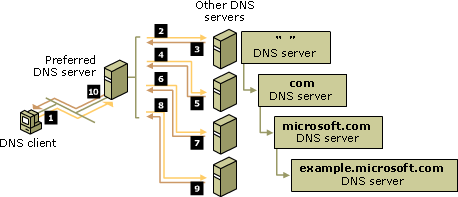
\includegraphics[scale=0.75]{imagenes/dns-system.png}
	\caption{Diagrama de operación del servicio DNS ilustrando comunicación entre servidores de dicho tipo.}
	\label{fig:dns}
\end{figure}

En la práctica, el servicio DNS emplea el protocolo UDP para la comunicación desde y hacia los servidores de dicho tipo, esto pues las características de una consulta DNS contemplan:

\begin{itemize}
\item \textbf{Consultas Auto-Contenidas} La información de una consulta DNS calza fácilmente en un paquete de UDP.
\item \textbf{Orden Irrelevante} Los requerimientos DNS no necesitan ser procesados en un orden establecido. Sin embargo, si requieren ser eventualmente procesados y ello en el menor tiempo posible. Un factor que justifica el uso de UDP al ser precisamente un protocolo orientado a mensajes.
\end{itemize}

De esta manera, las características anteriores justifican el uso de UDP como protocolo para la comunicación entre los servidores DNS.

El escenario antes descrito explica el por qué UDP tiene una participación de gran importancia en las redes actuales (en especial sobre Internet) y además, dado el sostenido aumento en el número de conexiones explicado en las secciones previas, da cuenta de cómo el tráfico de éste tipo de comunicación representa una porción muy significativa en la operación de las redes modernas. Una situación que con el paso de los años ha exigido cada vez mejores técnicas de procesamiento para dar mejores tiempos de respuesta.

\section*{Planteamineto de Investigación}

La pregunta natural entonces es: ¿Están capacitados los servidores DNS para responder tal cantidad de peticiones correctamente? Más allá de la respuesta a ésta interrogante el hecho es que, para su correcta operación, los servidores DNS deben garantizar bajos tiempos de respuesta y eficiencia en su operación en todo escenario.

Un excelente enfoque para abordar la problemática anterior mora en usar paralelismo, ósea, aprovechar la independencia entre peticiones DNS para procesar varios requerimientos a la vez de manera simultánea. En la práctica, dicha solución propone compartir una misma interfaz de conexión (denominada \emph{Socket}) entre varios hilos de ejecución. Ésta práctica supone --en teoría-- un incremento en el rendimiento de operación del procesamiento de las peticiones DNS, siempre que existan procesadores disponibles para atender cada hilo de forma independiente.

Sin embargo, los resultados al evaluar el enfoque antes propuesto revelan un preocupante e insospechado panorama donde el rendimiento de los servidores DNS no escala al incorporar directamente paralelismo en el procesamiento de peticiones como se esperaría \cite{tesis:diegoDCC}. Éste fenómeno ha sido repasado por distintos grupos de investigación en el área como Facebook, Toshiba \cite{post:facebook, paper:toshiba} e incluso industrias nacionales como NIC Chile, pero sin mayor solución más que delegar dicha responsabilidad a unidades estructurales del sistema operativo (como el kernel del sistema operativo) de donde tampoco se han conseguido mayores mejoras.

La pregunta entonces es ¿Por qué el sistema de procesamiento de peticiones DNS no escala al incorporar paralelismo directamente? Una sospecha interesante propone que probablemente el sistema de procesamiento de paquetes para UDP (que es el protocolo involucrado en las peticiones DNS) podría tener imperfecciones a nivel de diseño en el sistema operativo que no garantizarían su óptimo funcionamiento en condiciones de concurrencia, sugiriendo como responsable del problema a un defecto de contención a nivel de estructuras compartidas del sistema operativo. Sin embargo, dicha hipótesis no ha sido comprobada ni desmentida. Por otra parte, determinar la causa del problema anterior significa un tremendo desafío pues implica trabajar a nivel del núcleo del sistema operativo, que combina diversos paradigmas y enfoques de programación incorporados a lo largo de su desarrollo, unido a la dificultad inherente de trabajar analizando un sistema complejo como lo es el kernel mismo.

El presente trabajo plantea precisamente un estudio amplio que reune las principales sospechas de investigación vigentes del problema al momento de su desarrollo, de manera de identificar y analizar las distintas componentes responsables del problema detectado, así como también el estudio de alternativas para palear dicha situación.


\end{intro}
%\chapter{Primero}
\lipsum[1-3]
\begin{defn}[ver \cite{KAR00}] Definición definitiva $$\frac{d}{dx}\int_a^xf(y)dy=f(x).$$\end{defn}
%\chapter{Segundo}
\lipsum[50-60]
\chapter{Motivación y Antecedentes}

Como primer aspecto de la investigación es preciso contextualizar y limitar el caso de estudio que determina el problema objeto de la presente investigación. En el presente capítulo se repasarán los conceptos básicos para el común entendimiento del problema, y se ilustrará evidencia para apoyar la vigencia e importancia de estudio de la pregunta de investigación propuesta.

\section{Sistemas Operativos Modernos}
El paso del tiempo ha permitido a los fabricantes de hardware desarrollar componentes cada vez de mayor capacidad. Procesadores, memorias, tarjetas de videos, sistemas de almacenamiento, y prácticamente todos los componentes de un computador han evolucionado en capacidad, un escenario que ha impulsado a los desarrolladores de sistemas operativos a generar plataformas más robustas y eficientes a la hora de aprovechar toda la nueva amalgama de recursos disponibles en cada nueva generación de componentes. Una de las características más notables para esta industria sin duda ha sido la \textbf{capacidad multiprocesador} o bien denominada \emph{SMP}\footnote{Por sus siglas en inglés: \textit{Symmetric Multi-Processor System}}.

A finales de la década de los 80, los fabricantes de microprocesadores hicieron uno de los saltos más significativos en la industria al promover una nueva arquitectura de hardware que postuló un nuevo enfoque de aprovechamiento del procesador, incorporando varios de los mismos en un esquema que planteaba como siguiente paso la idea de disponer múltiples procesadores en una máquina, de manera de delegar tareas para su ejecución simultánea. Este enfoque permitió llevar a la práctica por primera vez la técnica del paralelismo en el software.

El primer enfoque arquitectural masivo para el paralelismo se denominó como la arquitectura \textbf{Front Side Bus} (FSB, ver figura \ref{fig:FSB}), muy popular entre procesadores de la línea Intel Core 2 Duo y Atom. Éste enfoque planteó la disposición de varios procesadores físicos, cada uno con recursos propios de memoria caché local los cuales se interconectaban por un canal de comunicación común, el cual daba acceso a la memoria completa del sistema y al resto de los recursos del mismo. El problema de esta arquitectura era que para que un procesador pudiese emplear el bus de datos, necesariamente el mismo debía estar libre de comunicaciones de cualquier otro procesador, problema que al poco tiempo que las memorias aumentaron su capacidad evidenció un efecto de cuello de botella inherente a éste diseño.

\begin{figure}[th!]
\centering
\subfigure[Arquitectura \emph{FSB}]{
	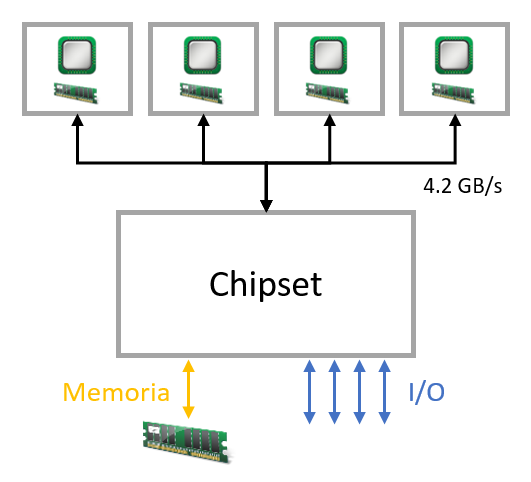
\includegraphics[width=.3\textwidth]{imagenes/FSB.png}
	\label{fig:FSB}
}
\subfigure[Arquitectura \emph{DIB}]{
	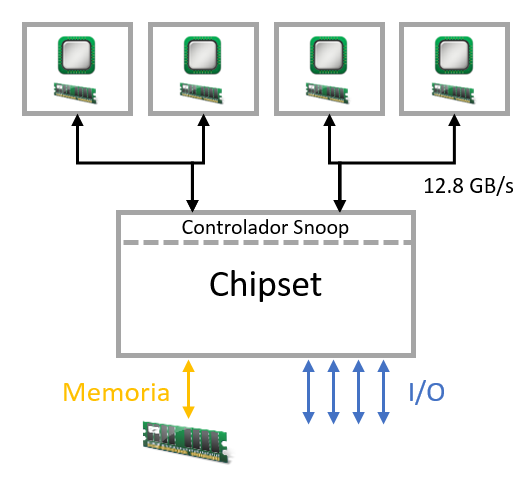
\includegraphics[width=.3\textwidth]{imagenes/DIB.png}
	\label{fig:DIB}
}
\subfigure[Arquitectura \emph{DHSI}]{
	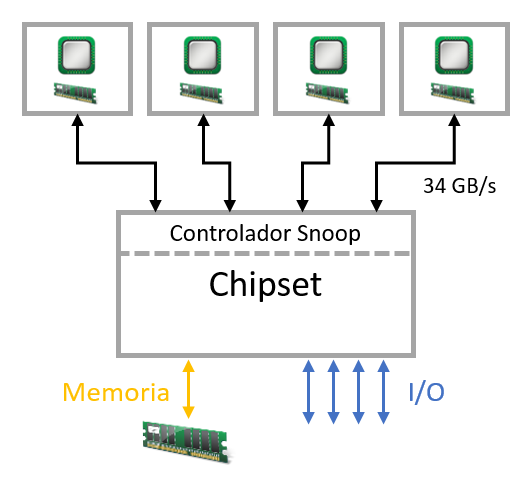
\includegraphics[width=.3\textwidth]{imagenes/DHSI.png}
	\label{fig:DHSI}
}
\caption{Diagrama de las distintas arquitecturas de hardware para la comunicación de múltiples procesadores.}
\label{fig:arquitecturas}
\end{figure}

Con objeto de explotar mejor el potencial de un esquema multiprocesador se desarrollaron varios rediseños del esquema FSB con el fin de eliminar el punto de contención en el bus compartido. Así es como surgieron las arquitecturas \textbf{Dual Independent Bus} y \textbf{Dedicated High-Speed Interconnects} (imagen \ref{fig:DIB} y \ref{fig:DHSI} respectivamente) que postulan un enfoque similar a FSB pero garantizando un canal exclusivo para cada procesador o grupo de procesadores del sistema. Una mejora inmediata de estos enfoques con respecto a FSB corresponde a un significativo aumento de las velocidades de transferencia, esto de la mano de que con canales cada vez más exclusivos por CPU se consiguen mejores velocidades en la comunicación general. Sin embargo, estas modificaciones revelaron otro aspecto a considerar: En sistemas SMP, y básicamente en cualquier sistema que teóricamente plantee la capacidad de procesamiento paralelo, deben haber mecanismos de control de consistencia de los datos que permitan mantener un registro coherente de los valores almacenados en distintas porciones del sistema. Vale decir, como los esquemas de procesamiento múltiple emplean procesadores provistos tanto de memoria local como de memoria compartida, se deben emplear mecanismos que garanticen la consistencia y coherencia de los valores que tengan presencia en diferentes locaciones del sistema. A dicho conjunto de esquemas de control de valores se les denomina \emph{protocolos de coherencia de cache} y son los que dan flexibilidad en un sistema para que la memoria local de un procesador disponga de valores coherentes con la más reciente modificación de dicho valor, aun habiendo ocurrido ésta modificación en otro núcleo de procesamiento.

\begin{figure}[!h]
	\centering
	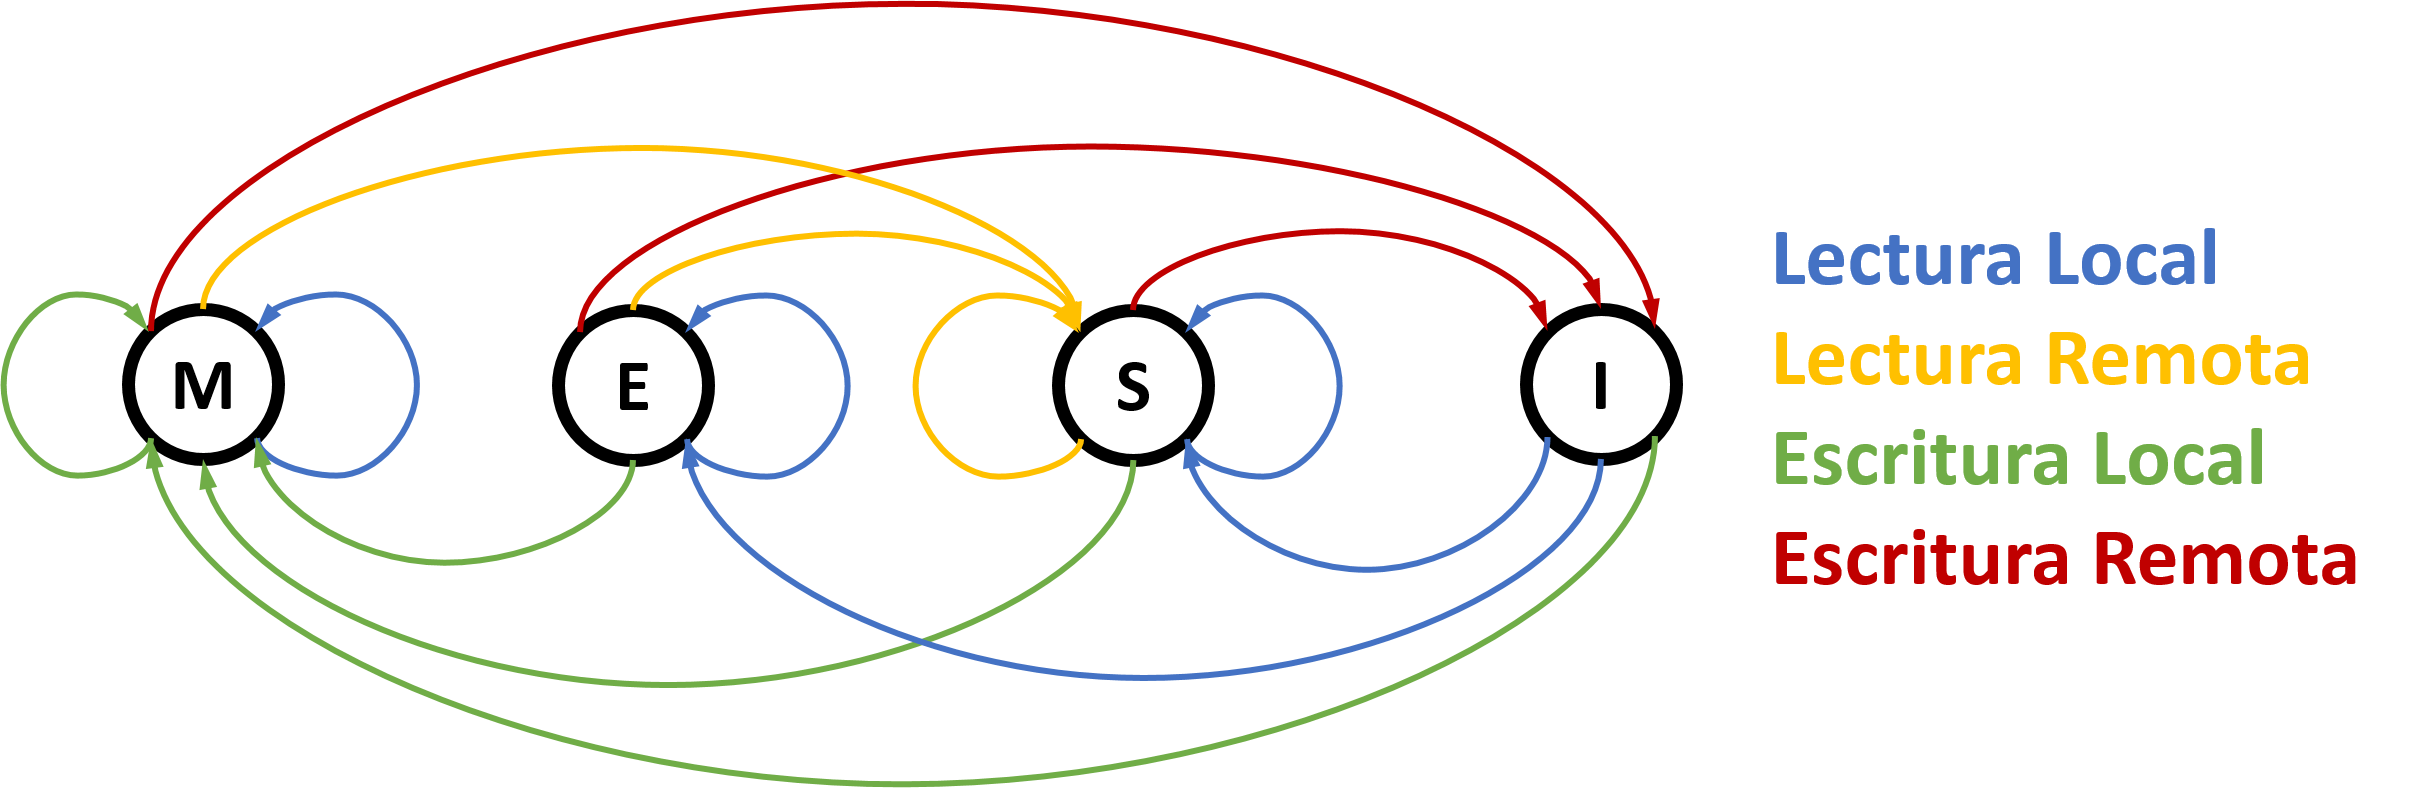
\includegraphics[scale=0.3]{imagenes/MESI.png}
	\caption{Diagrama de transiciones del protocolo MESI.}
	\label{fig:MESI}
\end{figure}

%\begin{center}
%\begin{tikzpicture}[scale=0.13]
%\tikzstyle{every node}+=[inner sep=0pt]
%\draw [black] (10.3,-21.8) circle (3);
%\draw (10.3,-21.8) node {$M$};
%\draw [black] (29.9,-21.8) circle (3);
%\draw (29.9,-21.8) node {$E$};
%\draw [black] (50.5,-21.8) circle (3);
%\draw (50.5,-21.8) node {$S$};
%\draw [black] (70.6,-21.8) circle (3);
%\draw (70.6,-21.8) node {$I$};
%\draw [black] (11.517,-19.059) arc (153.39789:26.60211:32.358);
%\fill [black] (69.38,-19.06) -- (69.47,-18.12) -- (68.58,-18.57);
%\draw [black] (9.739,-24.735) arc (16.90501:-271.09499:2.25);
%\fill [black] (7.63,-23.14) -- (6.72,-22.89) -- (7.01,-23.85);
%\draw [black] (52.948,-20.074) arc (119.61129:60.38871:15.386);
%\fill [black] (68.15,-20.07) -- (67.7,-19.24) -- (67.21,-20.11);
%\draw [black] (31.697,-19.4) arc (139.64058:40.35942:24.348);
%\fill [black] (68.8,-19.4) -- (68.67,-18.47) -- (67.9,-19.11);
%\draw [black] (68.363,-23.79) arc (-54.70403:-125.29597:13.522);
%\fill [black] (52.74,-23.79) -- (53.1,-24.66) -- (53.68,-23.84);
%\draw [black] (68.442,-23.882) arc (-49.11238:-130.88762:27.792);
%\fill [black] (32.06,-23.88) -- (32.34,-24.78) -- (32.99,-24.03);
%\draw [black] (51.823,-24.48) arc (54:-234:2.25);
%\fill [black] (49.18,-24.48) -- (48.3,-24.83) -- (49.11,-25.42);
%\draw [black] (49.177,-19.12) arc (234:-54:2.25);
%\fill [black] (51.82,-19.12) -- (52.7,-18.77) -- (51.89,-18.18);
%\draw [black] (32.324,-20.04) arc (120.44489:59.55511:15.543);
%\fill [black] (48.08,-20.04) -- (47.64,-19.2) -- (47.13,-20.07);
%\draw [black] (12.237,-19.511) arc (136.33228:43.66772:25.109);
%\fill [black] (48.56,-19.51) -- (48.37,-18.59) -- (47.65,-19.28);
%\draw [black] (28.577,-19.12) arc (234:-54:2.25);
%\fill [black] (31.22,-19.12) -- (32.1,-18.77) -- (31.29,-18.18);
%\draw [black] (7.601,-20.517) arc (272.30317:-15.69683:2.25);
%\fill [black] (9.68,-18.88) -- (10.14,-18.06) -- (9.15,-18.1);
%\draw [black] (12.857,-20.239) arc (116.16519:63.83481:16.425);
%\fill [black] (12.86,-20.24) -- (13.8,-20.34) -- (13.35,-19.44);
%\draw [black] (48.372,-23.913) arc (-48.37501:-131.62499:27.057);
%\fill [black] (12.43,-23.91) -- (12.69,-24.82) -- (13.36,-24.07);
%\draw [black] (69.21,-24.458) arc (-30.18959:-149.81041:33.273);
%\fill [black] (11.69,-24.46) -- (11.66,-25.4) -- (12.52,-24.9);
%\end{tikzpicture}
%\end{center}


En lo que a estos protocolos respecta, el más popular en los sistemas modernos es el denominado protocolo \textbf{MESI}\footnote{También se le denomina protocolo Illinois, en sentido de la universidad del mismo nombre.} \cite{paper:MESI}, denominado así por las iniciales de las palabras en inglés: \textbf{M}odified (Modificado), \textbf{E}xclusive (Exclusivo), \textbf{S}hared (Compartido) e \textbf{I}nvalid (Inválido). Es un protocolo que plantea un diagrama de estado (basado en los 4 estados que componen su nombre) para cada linea de memoria caché con información almacenada, a modo de mantener su integridad en el sistema frente a modificaciones que realice algún procesador (ya sea dueño de dicho banco de memoria o no). En conjunto con el protocolo \emph{MESI} existe la técnica \textbf{Buss Snooping} \cite{paper:snoop} que consiste en un esquema de coordinación para interceptar, notificar, modificar y coordinar los valores de memoria a medida que se van realizando cambios de los mismos por una determinada tarea. En conjunto, el protocolo \emph{MESI} y la operación del \emph{Bus Snooping} hacen posible las operaciones paralelas en entornos multiprocesador, proveyendo un ambiente adecuado para programar aplicaciones con ejecución verdaderamente paralela al brindar una capa de abstracción suficientemente flexible para aprovechar ésta técnica.

\subsection{Programación Multi-Hilo}
En la práctica, existen distintas maneras de conseguir paralelismo a la hora de programar un sistema. Los dos enfoques tradicionales es pensar en esquemas \textbf{multiproceso} (denominados procesos pesados) y \textbf{multihilo} (denominados procesos ligeros), diferenciados principalmente porque los primeros disponen de espacios de memoria disjunto entre ellos, no así los segundos. La programación multi-hilo es muy usada en aplicaciones por ser un enfoque probado y de fácil adopción por el soporte que brindan los sistemas operativos modernos a través de librerías que incorporan llamadas a sistema para tales fines, una la más populares en entornos UNIX es \textbf{PThreads}.

PThreads\footnote{Especificación base de la IEEE \url{http://pubs.opengroup.org/onlinepubs/9699919799/basedefs/pthread.h.html}} (o \emph{POSIX Threads} de su nombre completo) es una interfaz prácticamente estándar de programación hoy entre sistemas UNIX, resultado del trabajo de diseñadores de sistemas operativos que a finales de los 80 se abocaron al desarrollo de sistemas escalables para las nuevas arquitecturas de multiprocesadores. Ésta interfaz provee funciones para gatillar y controlar hilos de ejecución creados a partir de un proceso padre. Los hilos se caracterizan por disponer de un espacio de memoria propio cada uno con información privada (Con valores como el puntero de instrucciones, el \emph{Stack} de memoria, etc.) además de compartir entre ellos otros elementos como  por ejemplo el espacio de direccionamiento, señales del sistema o descriptores de archivos, característica que permite cierta comunicación entre ellos. Son una forma liviana de proveer paralelismo con respecto a su símil multiproceso provista por las llamadas a sistema \verb=fork()= y \verb=exec()= que generan tareas con espacios de memoria disjuntos entre ellas. Aún siendo procesos denominados ``ligeros'' y de incorporar ciertas dificultades a la hora de concebir el diseño de una aplicación, el uso de hilos a la hora de programar permite postular a un importante beneficio como lo es la escalabilidad en sistemas multiprocesador, ello al permitir que los distintos hilos se ejecuten en distintos procesadores físicos logrando ganancias efectivas en los tiempos netos de ejecución al distribuir la carga en distintos núcleos de procesamiento.

En contraparte con lo anterior, la programación concurrente conlleva ciertas dificultades inherentes a su capacidad de ejecución simultánea. El desafío más importante es que obliga a cambiar el diseño de las aplicaciones, haciendo necesario el uso de criterios sofisticados para resolver problemas de sincronización y de acceso a secciones críticas inherentes a éste modelo de programación.


\subsection{Mecanismos de Sincronización del Sistema}
Una responsabilidad fundamental de los sistemas operativos modernos es asignar el uso de recursos a las aplicaciones y garantizar un entorno seguro para la ejecución de dichas aplicaciones en el sentido del acceso a datos o recursos del sistema. En ésta línea, garantizar \textbf{consistencia en los datos} es una labor crucial en esquemas modernos, capaces de generar escenarios de múltiples aplicaciones con acceso simultáneo a datos compartidos entre ellas. La característica de operaciones paralelas es una introducción al kernel de Linux desde su versión 2.6\footnote{En versiones previas del kernel, la operación por defecto del \emph{scheduler} del kernel era serializar las tareas con accesos simultáneos al sistema a través del uso del denominado \emph{Big Kernel Lock} \url{http://kernelnewbies.org/BigKernelLock}.} que apareció a la vez que se popularizaron los equipos con capacidad multi-procesador, lo cual introdujo un nuevo nivel de complejidad en la labor de los sistemas operativos, haciéndolos responsables de mantener la correcta consistencia de la información en los distintos niveles de memoria en un escenario de ejecuciones paralelas, problema conocido típicamente como de \emph{Secciones Críticas} \cite{paper:cachebouncing, paper:nonscalablelocks}.

Para proveer operaciones sobre los datos en escenarios concurrentes, los sistemas operativos modernos implementan mecanismos de sincronización que permiten garantizar consistencia en sus estructuras de datos, permitiendo así operaciones simultáneas sobre una determinada estructura, y brindando así el efecto de compartir una estructura entre distintos procesos para que la modifiquen coincidentemente. Procesos que en la práctica pueden estar ejecutándose en núcleos de procesamiento distintos.

Para ello, el hardware de las computadoras provee las denominadas \emph{Operaciones Atómicas de Bajo nivel}, que son un conjunto de herramientas básicas que permiten manejar escenarios de concurrencia. Estas mismas operaciones ya provistas son la base para las denominadas \emph{Primitivas de Sincronización de Alto Nivel}, las cuales son cruciales para la correcta implementación de programas multi-hilo o multi-proceso. A continuación se repasan las diferencias conceptuales entre cada tipo de primitiva de sincronización y se mencionan las implementaciones más importantes de cada una que atañen a la presente investigación \cite{book:SOConcepts}.

\begin{table}[]
\centering
\begin{tabular}{|c|c|}
\hline
\textbf{\begin{tabular}[c]{@{}c@{}}Primitivas de sincronización\\ de Bajo Nivel\end{tabular}} & \textbf{\begin{tabular}[c]{@{}c@{}}Primitivas de sincronización\\ de Alto Nivel\end{tabular}} \\ \hline
Memory barrier & Completion                                                                                    \\ \hline
Atomic operations & Semaphore                                                                                     \\ \hline
Synchronize with interrupts & Futex                                                                                         \\ \hline
Spin locks & Mutex                                                                                         \\ \hline
\end{tabular}
\caption{Algunos ejemplos de herramientas de sincronización de distinto nivel disponibles en sistemas Linux.}
\label{tab:syncTools}
\end{table}

\subsubsection{Operaciones Atómicas}
Corresponden a un conjunto de instrucciones provistas por hardware disponibles en ambientes multi-procesador las que, aun siendo ejecutadas simultáneamente en distintas CPU's, en la práctica son ejecutadas secuencialmente en un orden arbitrario. En este caso la exclusión mutua es provista usando variables de naturaleza \verb=boleanas= que se denominan \emph{lock}. Existen diversas implementaciones de operaciones de éste tipo siendo las más conocidas: \emph{Test-and-Set}, que valida una condición y si se cumple realiza una asignación, \emph{Swap}, que intercambia el valor contenido entre dos variables, etc.

\subsubsection{Semáforo}
La solución a la protección de secciones críticas provista por mecanismos de operaciones atómicas es difícil de generalizar para aplicaciones más complejas, como en el caso en que se tienen múltiples hilos de ejecución. En este punto, se emplea una nueva herramienta de sincronización: Los \emph{Semáforos}. Un semáforo es una estructura de sistema que lleva una cuenta de un entero que puede ser modificado por medio de las operaciones atómicas \emph{Wait} y \emph{Signal}, que permiten verificar una condición para luego hacer un decremento del contador interno del semáforo, y gatillar un incremento de dicho contador, respectivamente.

Para su uso, la idea es que los diferentes hilos o procesos paralelos que soliciten acceso a un recurso compartan una estructura semáforo que sirva como barrera de acceso al recurso mismo. El semáforo admite la entrada de nuevos hilos de ejecución a la sección crítica protegida mientras su contador sea mayor que cero. De ésta manera un proceso que no consigue acceso al recurso protegido por un semáforo cae en un estado de espera (o a modo dormido) donde no gasta recursos del sistema.

\subsubsection{Mutex}
Los \textbf{Mutex} -o Monitores en español- Son otra estructura de sincronización de alto nivel provista por el propio kernel (disponible en \verb=kernel/locking/mutex.c=). Su nombre es precisamente la sigla en inglés de \emph{\textbf{Mut}ual \textbf{Ex}clusion Object}, que provee una herramienta para dar exclusión mutua en acceso a un recurso. En la práctica, corresponde a un semáforo binario, permitiendo el acceso exclusivo de un hilo de ejecución a un recurso protegido.

\subsubsection{SpinLock}
Son las primitivas de sincronización de más bajo nivel disponible en los sistemas Linux para garantizar exclusión mutua. Su operación se basa en ciclos de espera denominados \emph{busy-waiting} que son ciclos de procesador muertos, donde no se hace más que verificar el cambio de una condición que en la práctica consiste en ``obtener'' el \emph{lock}. Esta lógica de operación hace de los spinlocks una herramienta de sincronización de cuidado pues su operación está pensada solo para secciones críticas ligeras (de pocas instrucciones). Se diferencia de las otras herramientas de sincronización pues es usada en entornos de código que no puede dormir y debe estar preparado para retomar su operación\footnote{Un ejemplo de éste tipo de códigos son los \textit{Handlers} de interrupciones, que deben estar siempre listos para manejar un evento.}. Los sistemas operativos modernos proveen esta estructura de sincronización y una completa interfaz de uso, disponible desde sus encabezados en \verb=include/linux/spinlock.h=.

Bien utilizados, los spinlocks son capaces de proveer un mejor desempeño que las otras estructuras revisadas. Por el contrario, es sabido que el mal uso de éste tipo de herramientas de sincronización produce degradaciones importantes en los tiempos de operación generales de todo el sistema, pues significa el consumo de recursos en ciclos de procesamiento desperdiciados sin trabajo real, lo que en la práctica se traduce en un bloqueo de un hilo de ejecución \cite{paper:nonscalablelocks, paper:cachebouncing}. Aun cuando las implementaciones modernas de sistemas operativos incluyen optimizaciones en el rendimiento de estas estructuras (ya sea con optimizaciones energéticas o mejoras de scheduling \cite{paper:cacheaffinity}) lo cierto es que la naturaleza inherente para brindar sincronización de los spinlocks es por medio del mecanismo de \emph{busy-waiting}, que significa desperdiciar ciclos de reloj sólo esperando.

Los spinlocks son una de las estructuras de sincronización preferidas a la hora de solucionar escenarios de concurrencia en otras estructuras desplegadas en el kernel\footnote{Empleadas en estructuras de colas de almacenamiento de datos, módulos del kernel y los mismos sockets de Internet de Linux, entre otros.}, siempre tratando de mantener el cuidado de resguardar sólo regiones de código acotadas que no arriesguen el desempeño general del sistema en contextos de concurrencia.


\subsection{Sockets en Linux}
El modelo OSI ha estipulado a la familia de los protocolos TCP/IP como un estándar a la hora de establecer mecanismos de conexión entre computadoras. Sin embargo, las interfaces de programación no siguen la misma naturaleza estándar. Los distintos sistemas operativos implementan distintas interfaces públicas de aplicación para el uso práctico de TCP/IP. \textbf{Socket} es la denominación tradicional para las interfaces de programación que proveen los mecanismos para realizar tales conexiones. En otras palabras, es la interfaz que provee el sistema operativo para enviar mensajes a través de la red. En la práctica un socket representa una interfaz o punto de comunicación que maneja un protocolo de comunicación especifico. Los sockets operan bajo una dinámica denominada \emph{Cliente/Servidor} que dicta que la comunicación debe ser promovida por un cliente y atendida posteriormente por un servidor.

Los sockets en Linux \cite{rfc:147, book:sockets, paper:socketsGeneral} son estructuras que se construyen por medio de la llamada de sistema \verb=socket()=. Son estructuras provistas por el kernel del sistema\footnote{Típicamente implementada e importada desde el prototipo \verb=<sys/socket.h>=, disponible en los encabezados del kernel.} que al utilizarlos se manejan simplemente como descriptores de archivo, a pesar de que en su implementación a bajo nivel son bastante más complejos que una interfaz de sólo entrada y salida de datos. La gran diferencia de los sockets de Linux con respecto al común de mecanismos de entrada/salida por archivos es que los sockets están concebidos para una operación basada en un principio \emph{Cliente-Servidor}, lo que impacta finalmente en que su descriptor no apunta directamente a un archivo y su utilidad queda determinada sólo desde el momento en que se complete la dinámica de llamadas a sistema que hagan se establezca una conexión efectiva, ello dependiendo del protocolo a usar (Ver imagen \ref{fig:socketHandshake}). Linux cuenta con una API que provee métodos de comunicación sencillos para la manipulación de los sockets de acuerdo al protocolo para el que se configure el mismo.

\begin{figure}[h!]
	\centering
	\hspace*{\fill}
	\subfigure[Llamadas de sistema en esquemas de comunicación orientados a la conexión, como el caso de TCP.]{
		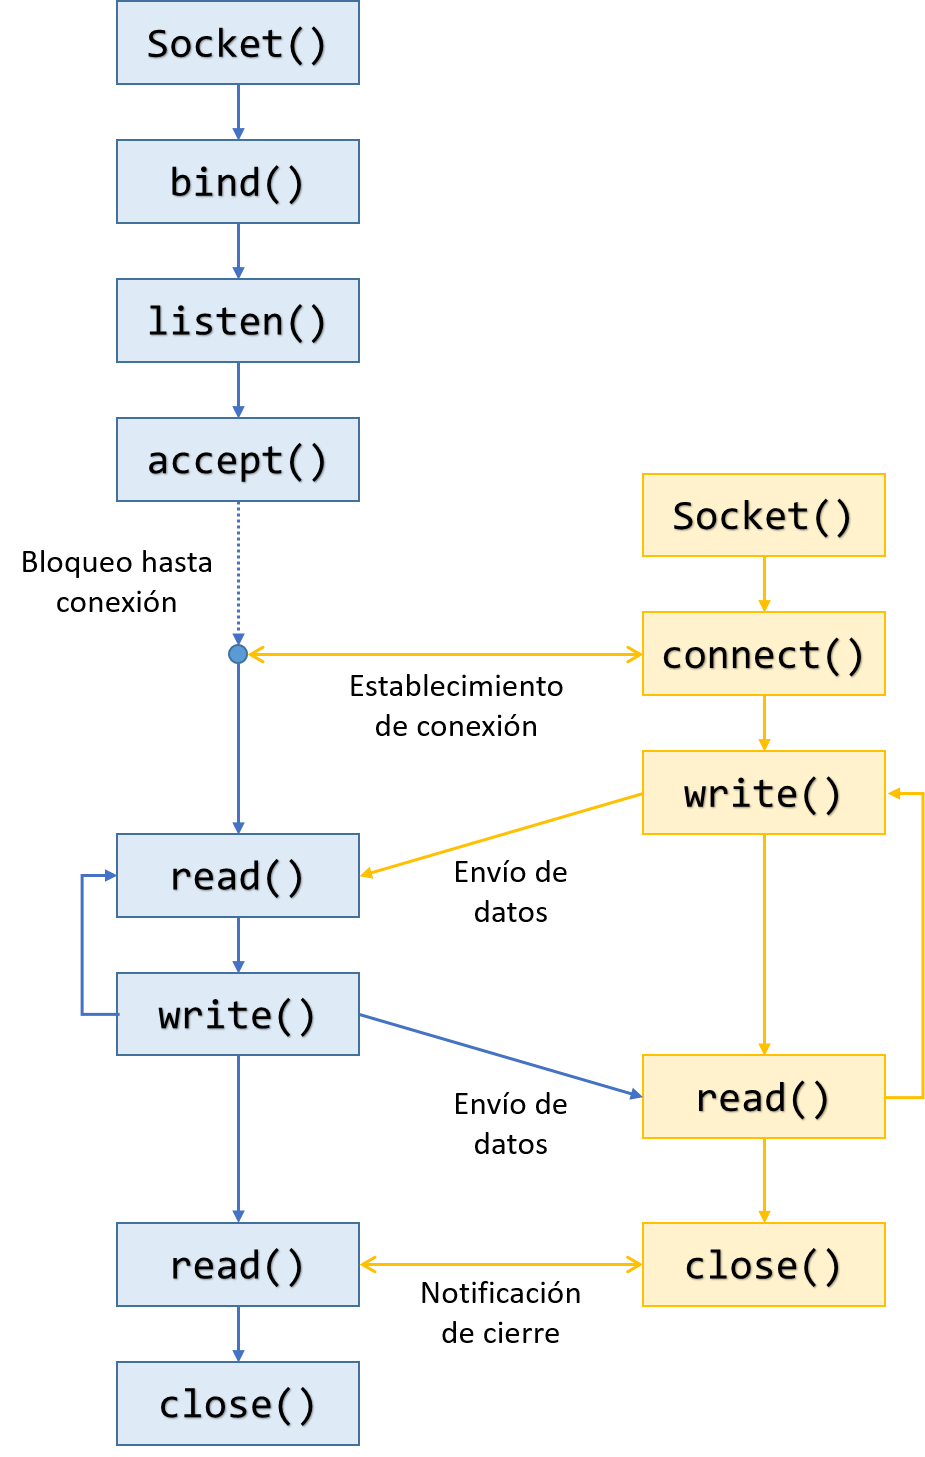
\includegraphics[width=.4\textwidth]{imagenes/llamadasTCP.png}
	}\hfill
	\subfigure[Llamadas de sistema en esquemas de comunicación orientados a la mensajería, como el caso de UDP.]{
		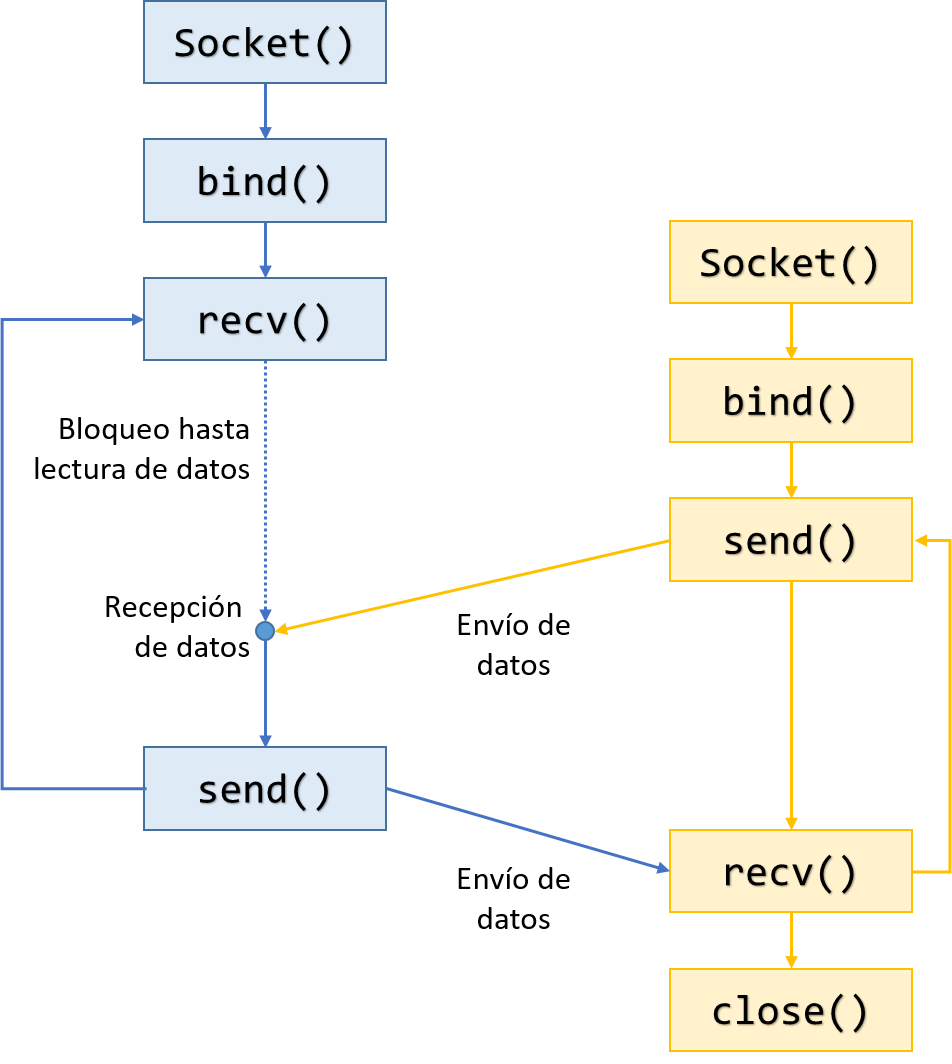
\includegraphics[width=.4\textwidth]{imagenes/llamadasUDP.png}
	}
	\caption{Un esquemático de las llamadas a sistema que se deben suceder para establecer una conexión \cite{book:sockets}. En éste caso, los componentes amarillos representan el lado cliente y aquellos azules representan el lado servidor en la dinámica de conexión.}
	\label{fig:socketHandshake}
	\hspace*{\fill}
\end{figure}


El sistema operativo reconoce a los diferentes sockets en operación a través de sus detalles de conexión de red, ello por medio de tuplas que contienen información de la conexión que provee el mismo. Una tupla congrega datos como: El protocolo de comunicación, las direcciones local y remota (con información de las capas de red y de transporte para la identificación del punto de acceso) y los identificadores de procesos local y remoto propietarios del punto de comunicación.

Los sockets son elementos muy versátiles en cuanto a su manipulación y uso. Se pueden usar en dos variantes principales que determinan el \emph{dominio del socket}:
\begin{description}
\item[Unix Sockets] Corresponden a un tipo de punto de comunicación que proveen los sistemas UNIX para realizar comunicación entre procesos de un mismo host.
\item[Internet Sockets] Son otro tipo de sistema de puntos de comunicación provistos en sistemas UNIX, basados en proveer una interfaz simple para implementar mecanismos de comunicación sobre una red.
\end{description}

Para las variedades recién mencionadas hay que sumar la capacidad de configuración de un socket. La primera y más importante es la configuración del modo de conexión que rige la dinámica de comunicación del socket: El \emph{protocolo de comunicación}. En éste apartado existen dos variantes comúnmente usadas: \verb=SOCK_STREAM= y \verb=SOCK_DGRAM= para usar TCP o UDP respectivamente. Sumado a lo anterior, los sistemas Linux proveen de la llamada de sistema \verb=setsockopt= que permite modificar características de una instancia socket, activando ciertas funcionalidades específicas o habilitando implementaciones con modificaciones especiales con respecto al funcionamiento estándar.

Más allá de la configuración puntual de la que se dote a un socket, la estructura interna de éste elemento es estándar y tiene especificaciones importantes de comentar para comprender su funcionamiento y posibles limitaciones.


\subsubsection{Estructura Interna}
Los socket de Linux están definidos como una estructura en el núcleo del sistema en \verb=include/linux/net.h= (ver figura \ref{fig:socketAnathomy}). En primera instancia, esta estructura incluye datos de su estado, información de su funcionamiento activo, etc. E incorpora dos sub estructuras fundamentales: \verb=proto_ops= que hace un nexo de punteros para con todas a aquellas funciones relacionadas a la manipulación del socket en su interacción de funcionamiento, implementando las funcionalidades mismas del socket. Y \verb=sock=, que contiene otras estructuras importantes en el funcionamiento correcto del socket, por ejemplo, estructuras usadas para el tránsito de los paquetes que por ellos circulan. Definida en ésta última estructura, cada socket posee 3 colas de tránsito que se usan para los procesos de encolamiento y desencolamiento de paquetes al socket mismo:
\begin{description}
\item[Receive\_queue] Cola de almacenamiento para los paquetes recién arribados al socket.
\item[Write\_queue] Cola de almacenamiento de los paquetes previo al envío de los mismos por la conexión definida por el socket.
\item[Backlog\_queue] Cola de almacenamiento de paquetes usada para colectar paquetes recibidos cuando la \textbf{Receive\_queue} está bloqueada (ocupada).
\end{description}

\begin{figure}[!h]
	\centering
	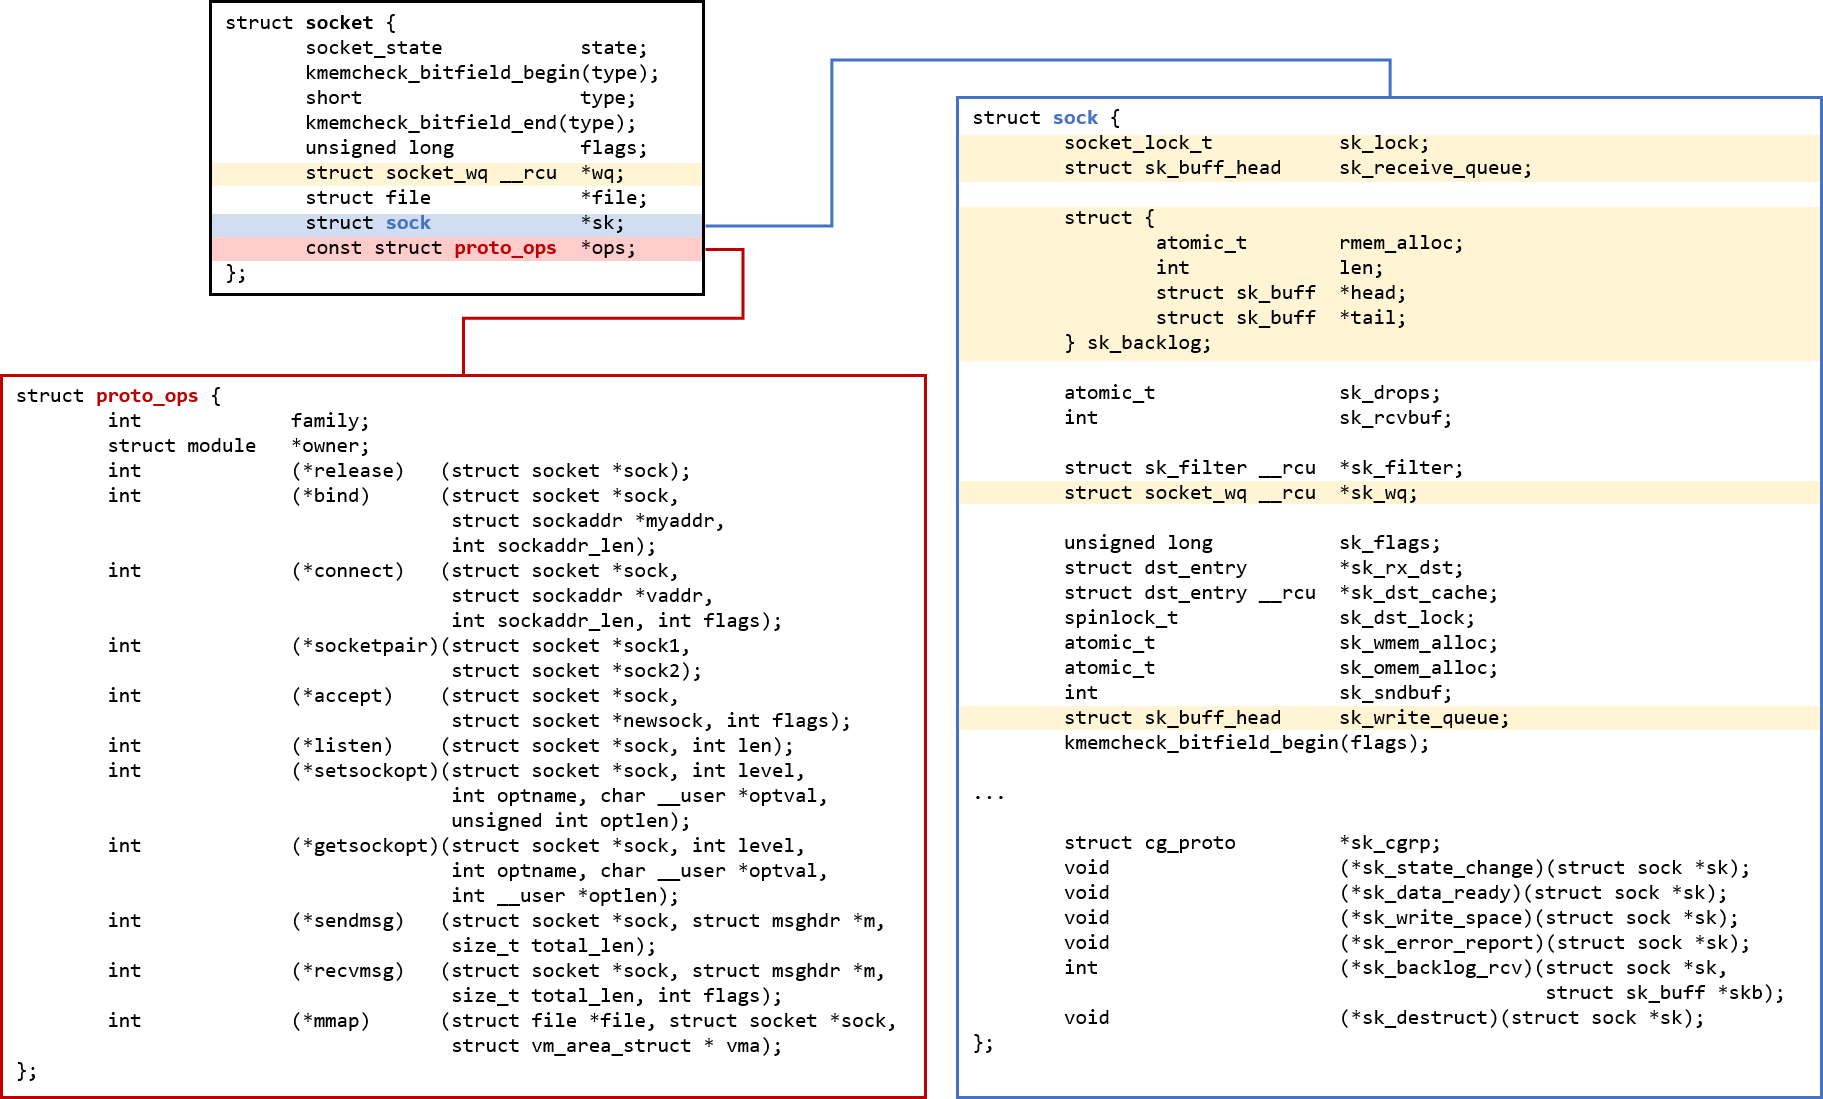
\includegraphics[scale=0.53]{imagenes/socketStructsDependecy.png}
	\caption{Diagrama de dependencias de la estructura interna de un Internet socket de Linux.}
	\label{fig:socketAnathomy}
\end{figure}

En términos de sus protecciones, los Internet sockets emplean spinlocks como herramientas de sincronización en el acceso a las estructuras internas que participan en los procesos de encolamiento y desencolamiento de paquetes (Ver figura \ref{fig:socketAnathomy2}). Específicamente, se reconocen dos capas de protección: Una primera capa, dada por un spinlock general en el acceso al socket, y un segundo nivel de protección dado por limitaciones de acceso a cada una de las 3 colas de paquetes que constituyen un Internet socket. Cada una de las 3 colas antes mencionadas posee su propio spinlock de protección frente a modificaciones concurrentes en pos de garantizar la integridad y coherencia de las operaciones sobre la misma.

\begin{figure}[!h]
	\centering
	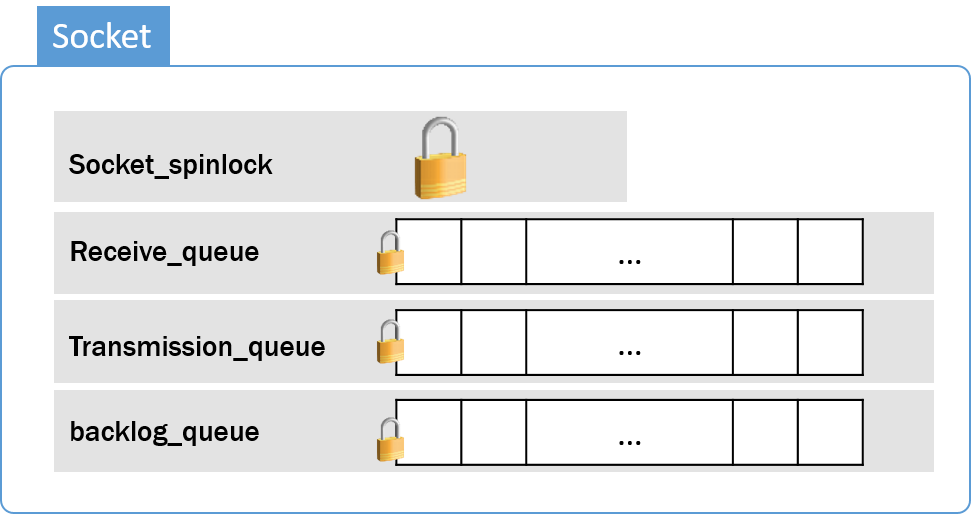
\includegraphics[scale=0.6]{imagenes/spinlocksSocket.png}
	\caption{Diagrama de niveles de protección presentes en un Internet socket de Linux.}
	\label{fig:socketAnathomy2}
\end{figure}

Por otro lado, el tránsito de un paquete que circula camino a un host puede ser descrito en una secuencia de pasos lógicos en que se interviene el mismo desde su arribo por una interfaz de red al llegar al socket:
\begin{enumerate}
\item Bloquear el socket usando el spinlock general de la estructura. De ésta manera se limitan las interrupciones para evitar concurrentemente encolamiento de otros paquetes.
\item Verificar si el lock está siendo usado por alguna aplicación de nivel usuario, en cuyo caso, se realiza el encolamiento del paquete directamente en la \textbf{Backlog\_queue}. Luego, para cada paquete:
	\begin{enumerate}
	\item Es procesado de acuerdo a las reglas de \emph{Netfilters}
	\item Son actualizadas las estadísticas del sistema, como \emph{Memory Accounting}.
	\item Se realiza el ingreso a la \textbf{Receive\_queue} (Esperando hasta la disponibilidad de su spinlock).
	\item Se hace una llamada al \emph{Scheduller} del sistema, para retomar procesos dormidos que hayan solicitado paquetes a éste socket.
	\end{enumerate}
\item Finalmente, se libera el spinlock general, continuando el proceso de recepción de los paquetes siguientes.
\end{enumerate}

\section{Presentación del Problema}
Como se mencionó en la sección \ref{section:dns}, el escenario advertido para los próximos años prevé un inmenso tráfico a Internet que podría llevar la cantidad de procesamiento del servicio DNS a varios órdenes de magnitud por encima de la carga actual \cite{slides:dnsRootQueries, paper:dnsRootQueries}. Es más, el panorama futuro postula que los dispositivos más avanzados serían muchísimo más versátiles en su operación pudiendo hacer un uso más agresivo y demandante de la red, realidad que se traduciría en más conexiones.

En este contexto, el servicio DNS --como pieza estructural de Internet-- debe estar preparado para enfrentar de la mejor manera posible la gran carga de procesamiento antes señalada, sobre todo dado que --por su naturaleza jerárquica-- éste servicio escala rápidamente el tráfico entre servidores. En estricto rigor, el sistema de DNS debe garantizarse eficiente en cualquier escenario.

A modo de preparativo para el escenario anterior, distintas instituciones han trabajado en alternativas para mejorar el procesamiento de las peticiones DNS a fin de optimizar su operación y tiempos de respuesta. Una apuesta para otorgar dicha mejora en performance y en línea con la tendencia actual de multiplicar el poder de procesamiento añadiendo más núcleos, consiste en incorporar paralelismo en el procesamiento de las consultas. Para ello se propone un esquema como el detallado en el diagrama de la ilustración \ref{fig:multi_thread} donde la idea consiste en que una misma maquina DNS pueda atender múltiples solicitudes de manera simultánea a través de una misma interfaz de red (en nuestro caso, un socket UDP). Este enfoque supone como principal mejora el escalamiento del procesamiento de peticiones DNS en un factor proporcional a la cantidad de hilos de ejecución atendiendo la interfaz compartida, ello siempre y cuando existan núcleos reales de procesamiento disponibles para los distintos hilos. Una proyección estimada se ilustra en la figura \ref{fig:proyeccionTeorica}. La tendencia de tiempos se rige de acuerdo a una logarítmica de acuerdo a la equitativa distribución de trabajos sobre los threads usados. Además se incluye un costo base inapelable correspondiente a los procesos de construcción y coordinación del sistema en los mecanismos de control de la prueba.

\begin{figure}[]
	\centering
	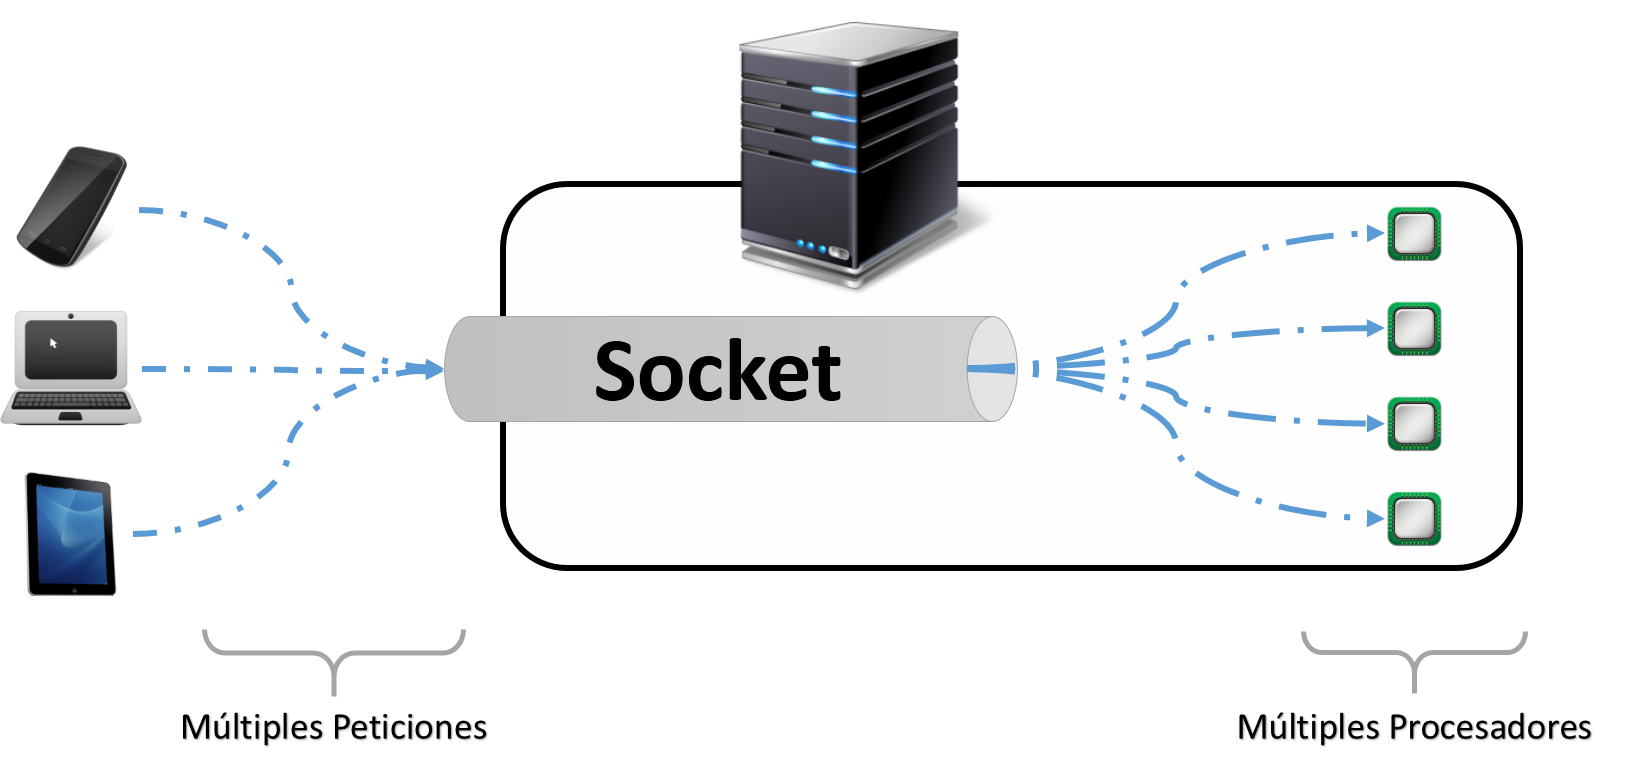
\includegraphics[scale=0.45]{imagenes/conf_multi_thread}
	\caption{Esquema de procesamiento multi-thread en un servidor con 4 procesadores reales, empleando un hilo por procesador. Escenario que en teoría, supone un mejor desempeño general, más no lo consigue en la práctica.}
	\label{fig:multi_thread}
\end{figure}

\begin{figure}[!h]
	\centering
	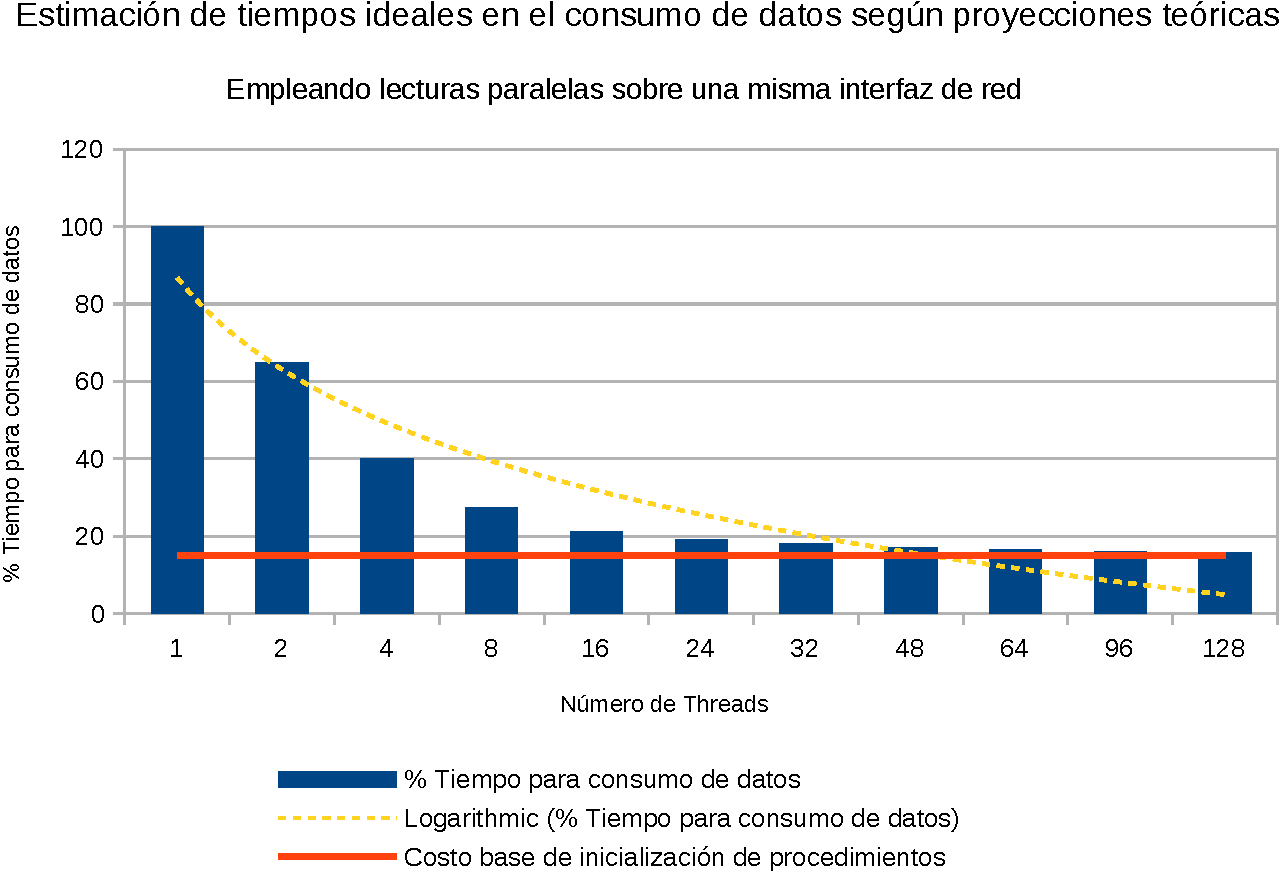
\includegraphics[scale=0.6]{resultados/proyeccionTeorica-crop.pdf}
	\caption{Estimación teórica de tiempos resultantes en el consumo de datos sobre una misma interfaz de red al incorporar lecturas paralelas.}
	\label{fig:proyeccionTeorica}
\end{figure}

Inspirados en la consistencia del argumento teórico detrás de la propuesta anterior, varias instituciones han evaluado este enfoque de procesamiento \cite{post:facebook, paper:toshiba}, pero con resultados poco alentadores. La experiencia local, de la mano de NIC Chile es un buen ejemplo del problema detectado. Aprovechando su infraestructura en pos de mejorar sus propios servicios, NIC Chile\footnote{Administrador del Top Level Domain \emph{.CL}} evaluó un diseño multi-hilos en el procesamiento de consultas DNS a sus servidores a fin de lograr una mejora de performance en su procesamiento DNS tal y como el diseño teórico anterior plantea sin sospechar el resultado real. En la práctica, el rendimiento final al incorporar paralelismo no estuvo ni cerca de las proyecciones esperadas y lejos de reducirse, los tiempos de procesamiento aumentaron con respecto al esquema sin multi-hilos, ello aun cuando no existían indicios de sobrecarga en las máquinas. Este resultado, inconsistente con el argumento teórico ya mencionado, planteó la duda sobre la verdadera capacidad de procesamiento paralela desde instancias de comunicación de red en sistemas multicore y en el sistema Linux per se.


\subsection{Validación del Problema}

El caso de estudio objeto de ésta investigación ya ha sido previamente analizado en trabajos recientes \cite{tesis:diegoDCC} rescatando importantes conclusiones como:
\begin{itemize}
\item Mostrar que al incorporar paralelismo por medio de threads y lecturas concurrentes a un socket UDP enfrentados a un escenario de saturación, no se logra mejora efectiva en los tiempos de consumo de datos.
\item Descartar la implementación de \emph{libc} como punto de problema, eliminando así posible responsabilidad de las llamadas de sistema como \emph{read} usadas en la lectura de sockets.
\item Mostrar la capacidad de mejoramiento del rendimiento de los sockets UDP por medio de modificaciones de bajo nivel en la estructura socket.
\end{itemize}

Sin embargo, dicho estudio planteó dudas importantes acerca de los elementos responsables del degradamiento de performance en escenarios multithreading, además de dejar latente la incertidumbre sobre cómo conseguir mejoras de performance de los socket, sin caer en modificaciones de la estructura misma. Elementos que son precisamente puntos de estudio de esta investigación.

Para ilustrar el interés y vigencia del problema antes descrito es necesario validar la persistencia del mismo en escenarios actuales que representen un caso típico de la problemática planteada, como viene siendo el caso de la comunicación entre servidores DNS. La dinámica DNS está caracterizada por una comunicación casi en su totalidad de tipo UDP, y cuya tendencia es creciente año a año, con una tendencia que se prevé se intensifique \cite{paper:dnsRootQueries,slides:dnsRootQueries}. De esta forma, se contempla un estudio de la situación actual del escenario multithreading en el consumo de datos desde una interfaz de red sobre UDP separando los dos contextos antes mendionados: \textbf{Hardware}, verificando el rendimiento en sistemas de arquitecturas de hardware diferente, y \textbf{Software}, estudiando el rendimiento en escenarios de ejecución basados en distintas versiones del kernel de Linux que son los que proveen el funcionamiento a estudiar.

En línea con lo anterior, se diseñó un \textbf{caso de estudio}\footnote{\url{https://github.com/sebablasko/Test_MultiThreadStressTransmision}} para evaluar el desempeño promedio de una interfaz de red representada por un socket UDP en el ejercicio de consumo de datos en un escenario de saturación. El modelo de la prueba incluye la evaluación del tiempo de consumo de una cantidad de datos de entrada correspondiente a 1 millon de paquetes de 512 bytes cada uno, emulando de esta manera un escenario clásico de congestión de un servidor de consultas DNS. En el caso de estudio se evalúan distintas configuraciones de threads consumiendo concurrentemente al mismo socket rescatando el tiempo total de consumo en cada caso. Para respetar la validez estadística de los resultados, la prueba anterior se repite un total de 60 veces por configuración de threads (Ver figura \ref{fig:testUDP}).

\begin{figure}[!h]
	\centering
	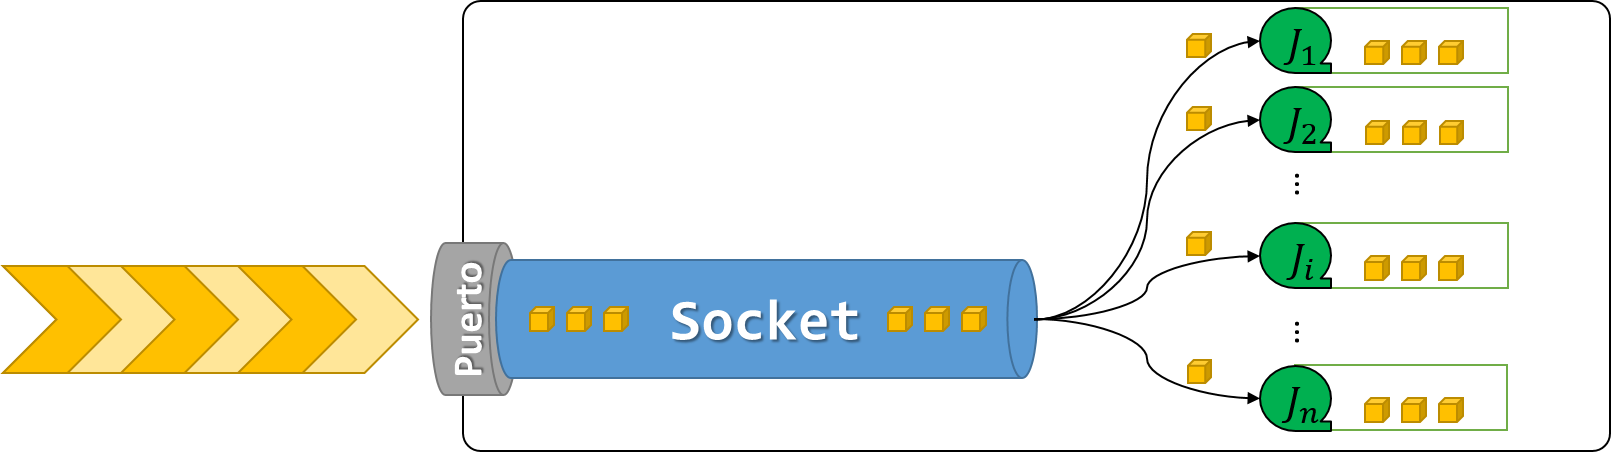
\includegraphics[scale=0.5]{imagenes/casoDeEstudio.png}
	\caption{Diagrama del \textbf{caso de estudio} que ilustra el diseño de la prueba de consumo de datos a través de un socket UDP usando múltiples hilos de ejecución.}
	\label{fig:testUDP}
\end{figure}

\subsubsection{Validación en Distintas Arquitecturas}

El comportamiento no escalable al usar threads es una característica que podría ser propia sólo de un tipo de arquitectura de recursos de hardware. Para comprobar el real alcance del problema antes descrito se evaluó la prueba de desempeño UDP en 3 escenarios de hardware diferente. Los tres escenarios de hardware se describen a continuación:

\begin{description}
\item[Laptop Dual Core] Laptop doméstico. Equipado con una CPU Intel(R) Core(TM) i5-5200U CPU @ 2.20GHz con tecnología \emph{hyperthreading} de Intel(R) y 6 GB de memoria. Un esquemático del sistema disponible en la figura \ref{fig:pc2}.
\item[PC Dual Socket] Computador de escritorio. Equipado cada socket con una CPU Intel(R) Xeon(TM) CPU @ 2.80GHz monocore, con tecnología \emph{hyperthreading} de Intel(R) y 2 GB de memoria interna. Imagen ilustrativa disponible en la figura \ref{fig:pc3}.
\item[Servidor 24 Cores Virtuales] Equipo servidor multiprocesador. Equipado con dos CPU Intel(R) Xeon(R) CPU X5660 @ 2.80GHz, cada uno hexacore, con tecnología \emph{hyperthreading} de Intel(R) y 24 GB de memoria, distribuidos en dos nodos NUMA de procesamiento, organizado en base a la \emph{Intel QuickPath Architecture}. Diagrama del sistema en imagen \ref{fig:pc1}.
\end{description}

\begin{figure}[h!]
	\centering
	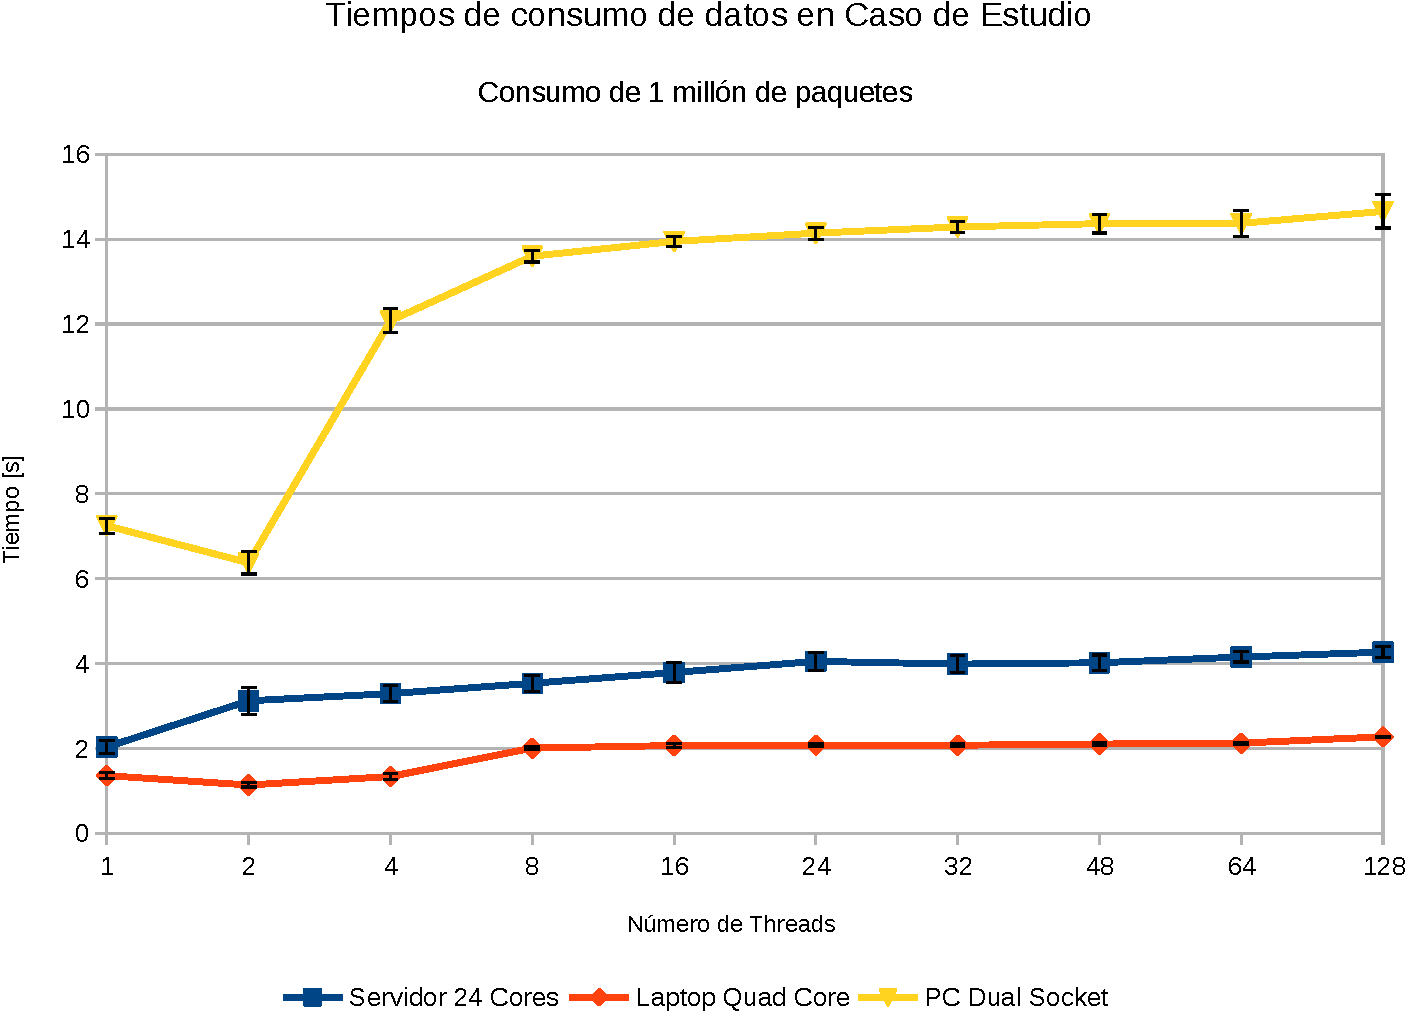
\includegraphics[scale=0.6]{resultados/transferenciaUDP1-crop.pdf}
	\caption{Grafico comparativo del rendimiento de prueba UDP entre distintas arquitecturas de hardware. Los valores mostrados son representativos de 60 repeticiones de la prueba de transferencia UDP.}
	\label{fig:tests_arch}
\end{figure}

\begin{figure}[h!]
	\centering
	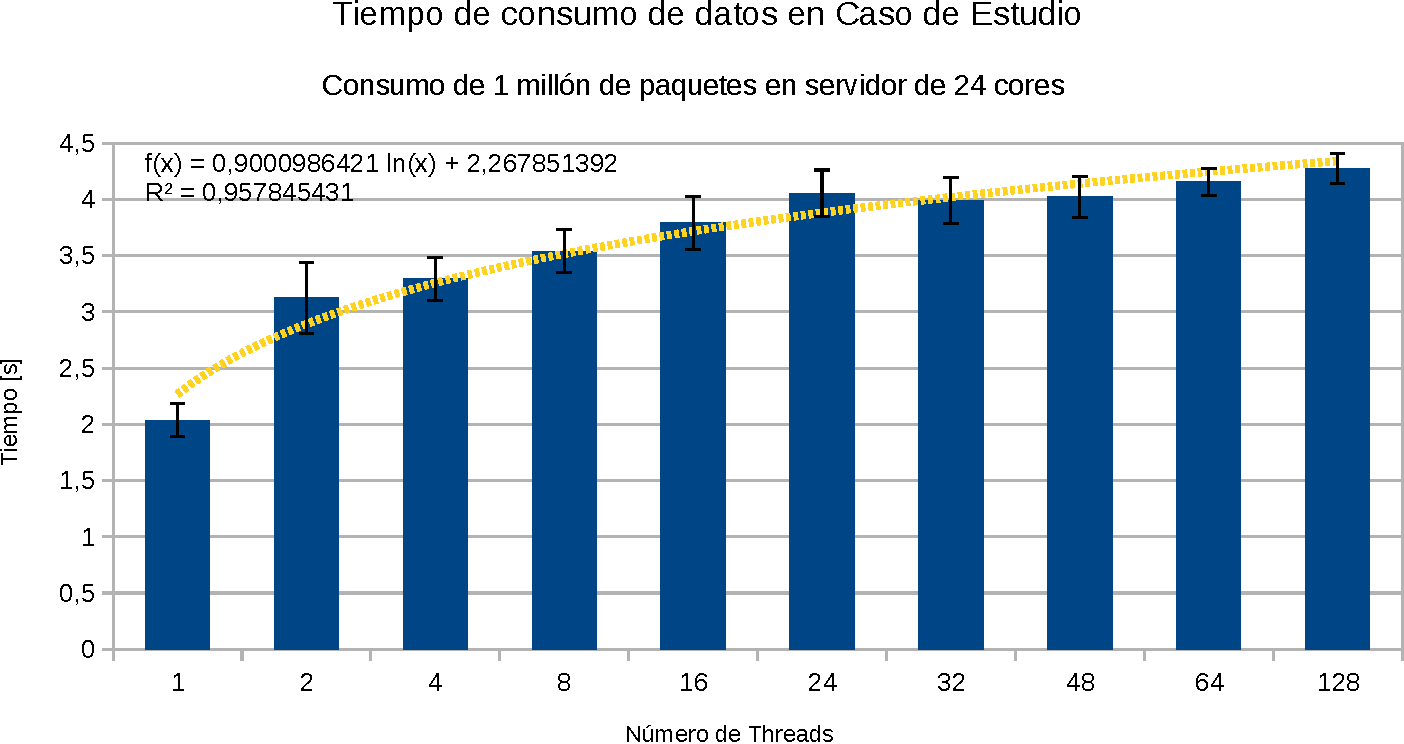
\includegraphics[scale=0.6]{resultados/transferenciaUDP2-crop.pdf}
	\caption{Gráfico de resultados de tiempo de consumo de datos en el caso de estudio presentado sobre la arquitectura del servidor de 24 cores representado por la figura \ref{fig:pc1}. La tendencia de resultados se ajusta a una curva logarítmica con un ajuste superior al 95\%.}
	\label{fig:tests_arch_detalle24}
\end{figure}

\begin{figure}
\centering
\hspace*{\fill}
\subfigure[Pc2]{
	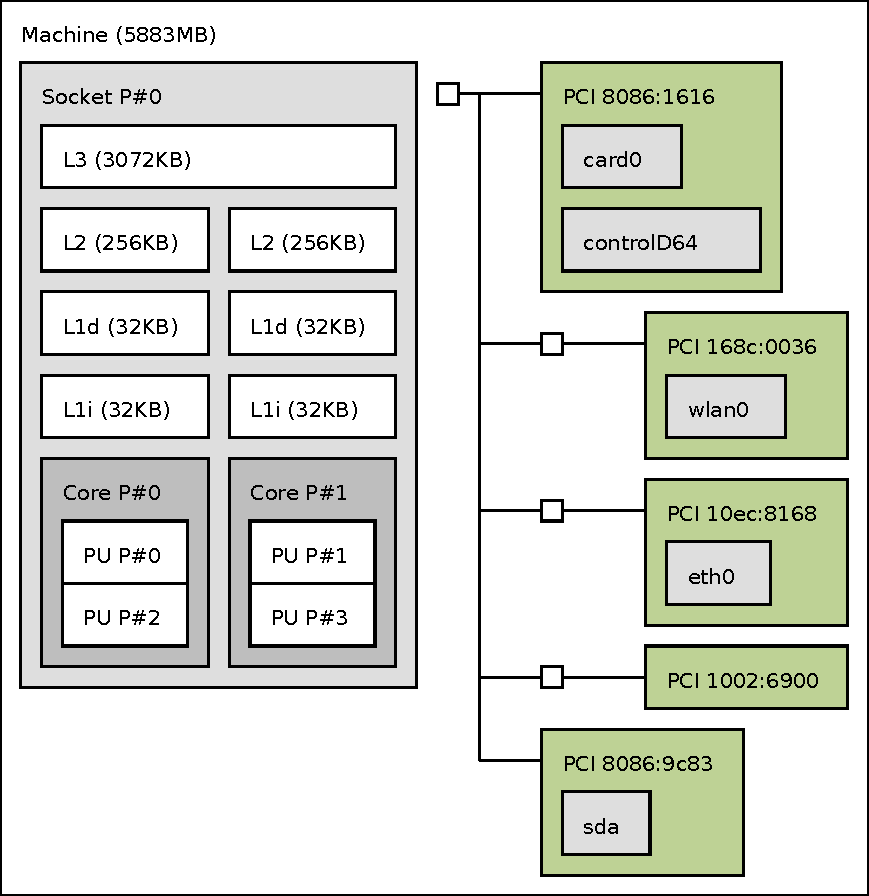
\includegraphics[height=.4\textwidth]{imagenes/pc2.pdf}
	\label{fig:pc2}
}\hspace*{\fill}
\subfigure[Pc3]{
	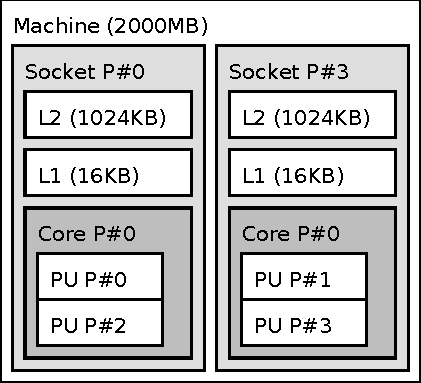
\includegraphics[height=.4\textwidth]{imagenes/pc3.pdf}
	\label{fig:pc3}
}
\hspace*{\fill}
\\
\subfigure[Pc1]{
	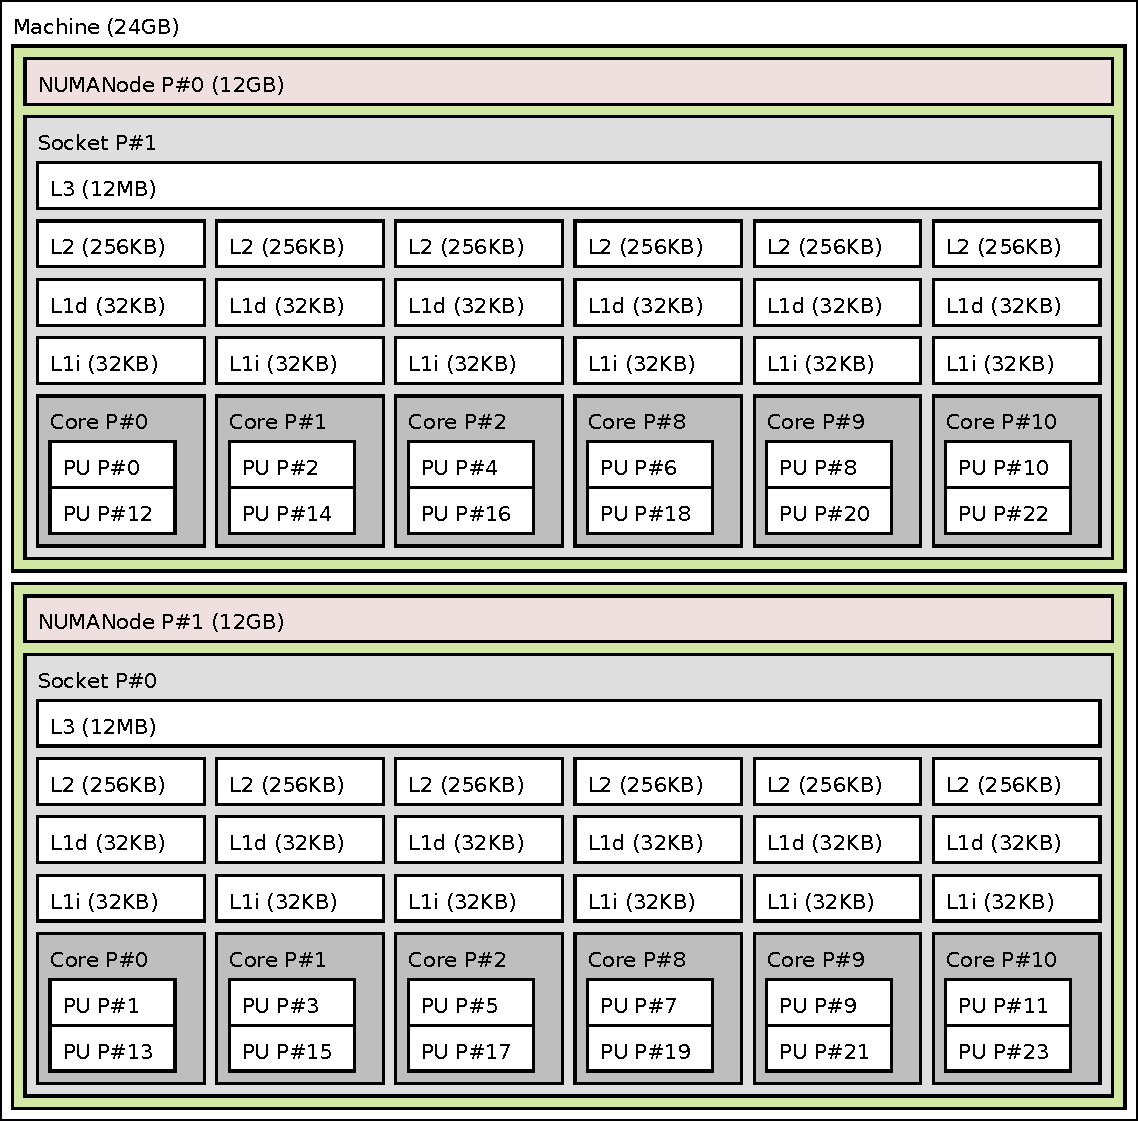
\includegraphics[width=.85\textwidth]{imagenes/pc1.pdf}
	\label{fig:pc1}
}
\caption{Esquemas de hardware de los 3 equipos evaluados para la validación del problema. Imágenes generadas con la herramienta \texttt{lstopo} del paquete \texttt{hwloc}.}
\end{figure}

De los resultados experimentales de la figura \ref{fig:tests_arch} se pueden rescatar dos aspectos relevantes:
\begin{itemize}
\item El primero, que el efecto de consumo concurrente es distinto entre los 3 escenarios estudiados, dejando en evidencia que las diferentes configuraciones de hardware en cada caso entregan diferente desempeño a la hora de aprovechar ejecuciones paralelas y de enfrentar escenarios de concurrencia.
\item El segundo, que el caso de mayor interés, ilustrado en la arquitectura del Servidor 24 Cores Virtuales, presenta una situación de baja de desempeño a medida que se congestiona (o satura) más fuertemente el consumo de la interfaz de red, representada por el socket UDP (Ver figura \ref{fig:tests_arch_detalle24}). La tendencia es similar a la reportada por estudios anteriores que cuestionan la aplicabilidad de técnicas de paralelismo en este tipo de arquitecturas por no demostrar un mejor desempeño evidente \cite{post:facebook, paper:toshiba, tesis:diegoDCC}.
\end{itemize}

Las conclusiones preliminares del estudio, apoyan la idea de continuar indagando la operación del caso de estudio en la arquitectura del servidor multiprocesador, que viene siendo el escenario típico para la operación DNS, que es el caso que nos inspira en esta investigación.

\subsubsection{Validación en Distintas Versiones de Kernel de Linux}

Al igual que con la arista de hardware, el fenómeno de mal rendimiento de threads detectado podría ser propio de la componente de software del sistema, entendido como una determinada versión del kernel de Linux. Una sospecha que se acentúa al recordar que parte importante del código fuente del núcleo es heredado entre versiones y que las versiones más populares del kernel abarcan una importante razón de tiempo entre sus publicaciones. A continuación se muestra una línea de tiempo con algunas de las publicaciones más importantes del kernel de linux\footnote{\url{https://www.kernel.org/category/releases.html}}.


\definecolor{myhighlight}{RGB}{250,250,60}
\begin{center}
\scalebox{1.2}{
\begin{tabular}{r |@{\timeline} l}
3 Diciembre 2009 & 2.6.32\\
4 Enero 2012 & \colorbox{myhighlight}{3.2}\\
20 Mayo 2012 & 3.4\\
30 Junio 2013 & \colorbox{myhighlight}{3.10}\\
2 Noviembre 2013 & \colorbox{myhighlight}{3.12}\\
30 Marzo 2014 & \colorbox{myhighlight}{3.14}\\
7 Diciembre 2014 & 3.18\\
12 Abril 2015 & \colorbox{myhighlight}{4.0.4}\\
\end{tabular}
}
\end{center}

Las versiones destacadas son aquellas que se consideraron como entornos de estudio interesantes para la validación del problema. La justificación de esta elección se basa en dos criterios: Primero, que el conjunto de versiones elegidas son todas \emph{Longterm Support} por lo que son la base principal en las ramas de desarrollo aledañas de otras versiones del kernel (sólo con correcciones de bugs importantes) y por lo tanto, son representativas de sistemas Linux más estables. Segundo, pues existen trabajos previos que ya se encargan de analizar el comportamiento estudiado en ediciones más antiguas del Kernel cómo en la versión base 2.6 \cite{tesis:diegoDCC}.

Para la evaluación, se instalaron las versiones destacadas de la línea de tiempo de kernels de Linux en un equipo de pruebas equipado con una CPU Intel(R) Core(TM) i7-4790 CPU @ 3.60GHz quadcore, dotado con tecnología \emph{hyperthreading} de Intel(R) y 8 GB de memoria, obteniendo así un equipo con 8 núcleos virtuales de procesamiento (Ver figura \ref{fig:desktop_kernel_pc}) y se registraron los distintos tiempos finales del caso de estudio planteado sobre cada versión del kernel contemplada. El objetivo de ésta prueba busca evidenciar si existe una tendencia constante en el tiempo resultante de la prueba entre las diferentes versiones del kernel, o si existe un punto de inflexión en las tendencias en algún cambio de versión. Un resultado comparativo de los distintos rendimientos entre versiones del kernel está ilustrado en la figura \ref{fig:tests_kernel}.

\begin{figure}[h!]
	\centering
	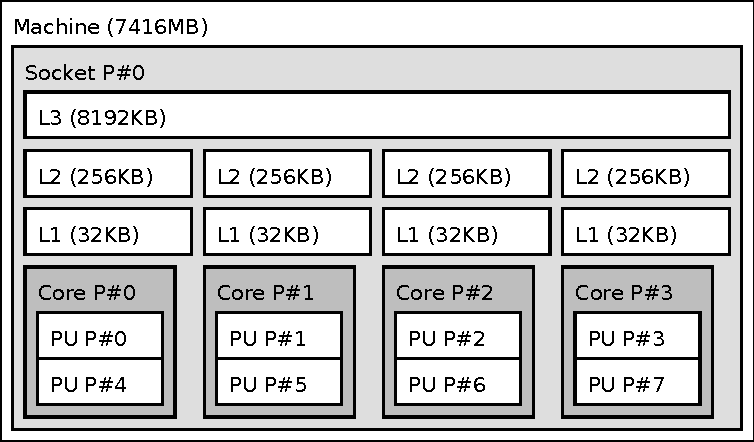
\includegraphics[scale=0.65]{imagenes/desktopkernelpc.pdf}
	\caption{Esquema de hardware del equipo donde se evaluó el rendimiento del caso de estudio sobre distintas versiones del kernel de Linux. El equipo corresponde a se compone de una }
	\label{fig:desktop_kernel_pc}
\end{figure}


\begin{figure}[h!]
	\centering
	\hspace*{\fill}
	\subfigure[]{
		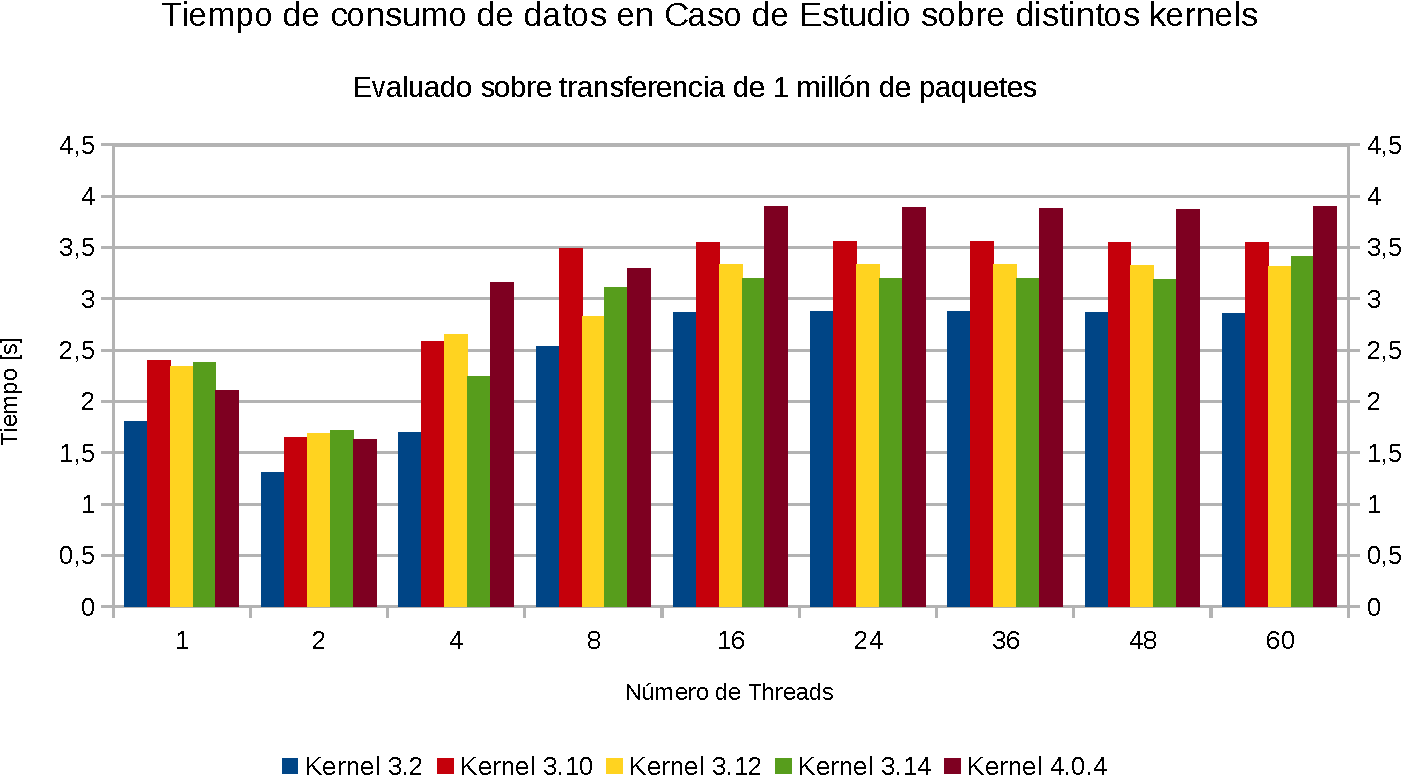
\includegraphics[width=.47\textwidth]{resultados/kernel1-crop.pdf}
		\label{fig:tests_kernel1}
	}\hfill
	\subfigure[]{
		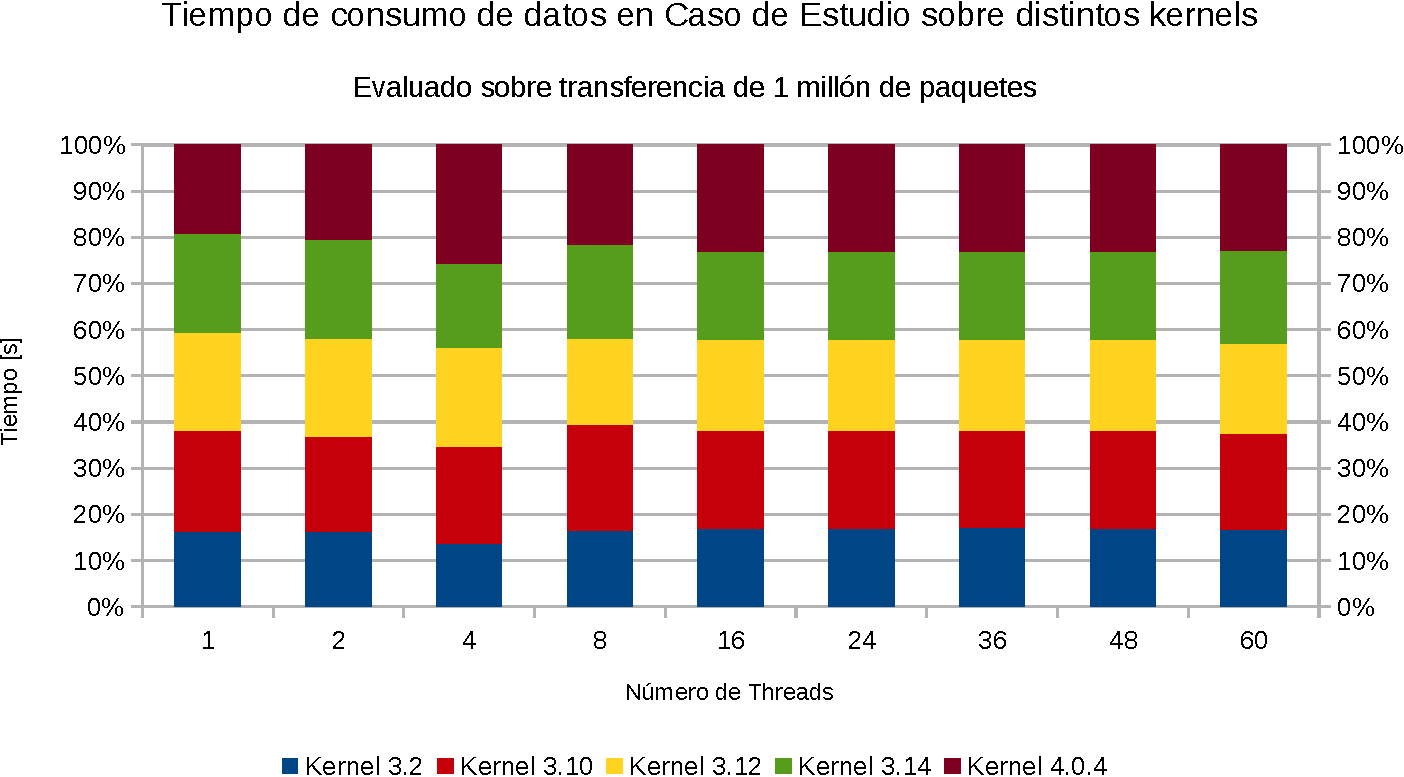
\includegraphics[width=.47\textwidth]{resultados/kernel2-crop.pdf}
		\label{fig:tests_kernel2}
	}
	\caption{Graficos comparativos del rendimiento de prueba UDP entre distintas versiones del Kernel. Los valores mostrados son representativos de 60 repeticiones de la prueba de transferencia UDP.}
	\label{fig:tests_kernel}
	\hspace*{\fill}
\end{figure}

Los resultados de esta prueba ilustran en primera instancia que las distintas versiones del kernel presentan distinto rendimiento sobre el caso de prueba estudiado, ello de acuerdo a los resultados del gráfico \ref{fig:tests_kernel1} dónde puede ser muy significativa la diferencia al incorporar threads en el consumo de datos.

En primer lugar, del gráfico de la figura \ref{fig:tests_kernel1} se desprende que las distintas versiones del kernel afectan el rendimiento final de la prueba, dándose el caso de que las versiones más antiguas del mismo registran menores tiempos generales en completar la prueba. Otro aspecto interesante es que, sin importar la versión del kernel que se está evaluando, el paso de uno a dos threads en el consumo de datos degrada fuertemente el tiempo total del la prueba, sumado a que no se ilustra ninguna mejora en los tiempos que sea proporcial al número de threads empleados en cada configuración de la prueba, dando a entender que el problema no ha sido corregido entre las versiones estudiadas.

Por otro lado, de acuerdo con el gráfico \ref{fig:tests_kernel2} donde se muestran las proporciones de tiempo correspondientes al consumo de datos del socket en cada configuración de hilos con respecto al tiempo total, se aprecian comportamientos idénticos entre las distintas configuraciones independiente del kernel usado. Esta situación muestra que a pesar de que los tiempos sean diferentes, las tendencias y comportamientos son uniformes entre las distintas versiones del kernel, por lo que la varianza de tiempos entre distintas versiones del kernel sería un fenómeno producido por ciertas optimizaciones o degradaciones del rendimiento en componentes que no son inherentes únicamente a nuestro caso de estudio. En otras palabras, el comportamiento o tendencia de tiempos registrados sólo se escala en un factor constante entre las distintas versiones de kernel estudiadas.

Los resultados anteriores terminan por validar la persistencia del problema descartando la responsabilidad del mismo a una única edición del kernel de Linux, y validando también la persistencia del problema mismo en arquitecturas de interés como lo son máquinas servidores multicore.

\subsection{Hipótesis del Problema}
Las sospechas iniciales del responsable de este problema apuntan a un defecto que se esconda a nivel del núcleo del sistema operativo \cite{paper:toshiba,post:facebook}. Como ya se mencionó, desde su versión 2.6 el kernel de Linux incorporó capacidad de procesamiento simétrico multiprocesador (\emph{Symmetric Multi-Processing - SMP}), con esto el scheduler de tareas transfirió los hilos de ejecución paralelos al mismo núcleo del sistema, con el costo de tener que implementar protección para áreas completas de código y estructuras a fin de evitar modificaciones concurrentes. Para ello, Linux provee diversas primitivas de sincronización mencionadas en secciones anteriores a disposición de los programadores.

La sospecha inicial apunta a que probablemente, el efecto encontrado al evaluar diseños como el de la ilustración \ref{fig:multi_thread} es precisamente reflejo de un problema a nivel del kernel, donde alguna estructura de sincronización de bajo nivel está presentando un problema de contención que se traduce en una serialización de acceso, o similar, y que repercute en tiempos muertos en casos de concurrencia. Una sospecha que es avalada por los resultados obtenidos hasta este punto de la investigación.

Una investigación realizada por Google \cite{slides:googleReuseport} ha llegado a establecer una colección de hipótesis consensuadas con otros importantes actores (como Facebook \cite{post:facebook}) concluyendo de que son varios los factores que contribuyen a la degradación generalizada que se presenta. En Primer lugar se postula un \textbf{punto de contención} generado a raíz de la compartición de la estructura socket entre varios hilos de ejecución, estructura que no estaría apropiadamente diseñada para sobrellevar un escenario de concurrencia como al que se expone en este caso. Otra teoría para explicar esta situación se basa en el fenómeno de los \textbf{rebotes de caché}, propios de un esquema \emph{SMP} pero que se vería acrecentado en situaciones como las descritas por la necesidad de mantener información estructural de los sockets entre varios hilos que se distribuirían entre los múltiples núcleos de procesamiento disponible. Una tercera línea apunta en atribuir las responsabilidades del mal desempeño a los \textbf{mecanismos de distribución de tareas} (El denominado schedulling para escenarios de distribución de carga) del sistema operativo, el cual en entornos \emph{SMP} jugaría en contra, degradando el rendimiento al modificar la propiedad de localidad de los datos para con los procesos constantemente, ello por medio de migraciones de los procesos entre las CPU disponibles. Otra hipótesis hace referencia a la posibilidad de que sean los propios \textbf{canales de comunicación} los que presentan un bajo rendimiento en situaciones de concurrencia como la descrita y cuyo overhead terminaría impactando en los tiempos netos, entre otros.

El problema real es que ninguna de las distintas hipótesis previamente repasadas ha sido experimentalmente estudiada, con lo que no se ha podido validar ni refutar la veracidad de las mismas. No tener claridad sobre cuál es la componente responsable incurre en otros problemas como el no poder postular una solución que consiga solucionar correctamente el mismo, al no tener claro cuál arista trabajar. En los capítulos siguientes se postula encapsular las hipótesis antes planteadas en líneas de investigación para corroborar experimentalmente la validez de las mismas, para posteriormente, con un entendimiento mejorado del problema, postular un mecanismo alterno que permita aprovechar la capacidad multiprocesador para lograr mejores tiempos netos en el caso de estudio ilustrado.

\subsection{Línea de Investigación}
Resumiendo lo anterior, la investigación vigente del fenómeno estudiado en el presente trabajo ha concluido por generar distintas hipótesis para explicar el mal rendimiento presentado por los Internet sockets de Linux en escenarios de concurrencia, más sin corroborar la validez de ninguna hipótesis experimentalmente. Las sospechas responsables de dicho problema se pueden agrupar en tres aristas distintas: Problemas de operación en primitivas del sistema, problemas de operación a nivel de canales de comunicación de hardware y problemas de operación en los mecanismos de administración de recursos y balanceo de carga. Serán justamente estas 3 líneas las que marcan las directrices de nuestra investigación. En los capítulos venideros se profundizará en cada una de dichas sospechas dando como cierre un veredicto acerca del grado de responsabilidad de la misma en cada caso.

%\chapter{Estudio del Problema}

Como se mencionó al final del capítulo anterior, la investigación vigente del fenómeno estudiado en el presente trabajo ha concluido en generar distintas hipótesis para explicar el mal rendimiento presentado por los sockets de internet en escenarios de concurrencia, más sin corroborar la validez de ninguna experimentalmente. Para ser exactos, y reiterando lo anterior, las sospechas se pueden agrupar en tres aristas distintas: Problemas de operación en primitivas del sistema, problemas de operación a nivel de canales de comunicación de hardware y problemas de operación en los mecanísmos de administración de recursos y balanceo de carga.

En el presente capítulo se estudian las tres líneas hipotéticas responsables del problema, inspeccionando en distintos niveles el funcionamiento del sistema, indagando en las operaciones teóricas de cada funcionamiento y contrastando dicho planteamiento a resultados experimentales obtenidos en cada caso. Es fruto de cada una de las siguientes subsecciones un análisis profundo del aspecto problemático estudiado, junto con una conclusión sobre el mismo. Así también, es fruto del presente capítulo un veredicto sobre cuales -Y en qué medida- de los problemas estudiados tienen verdadera responsabilidad en el fenómeno estudiado, de modo de confeccionar un marco de trabajo que nos permita empezar a postular enfoques de trabajo que paleen la problemática en cuestión.

\section{Estudio de Operación Primitivas de sincronización del Sistema}

La primera hipótesis a estudiar plantea que el bajo rendimiento de la operación de la interfaz de red -Ilustrada en nuestro caso de estudio por medio de sockets UDP- en escenarios de concurrencia, es causado por un mal desempeño de las estructuras que proveen los mecanismos de sincronización para dichos escenarios. Cómo se mencionó en el capítulo anterior, la capacidad multiprocesador de las computadoras modernas provee de un mayor poder de cómputo que se postula a ser aprovechado por medio del uso de técnicas de programación paralela, con el cuidado de que, en esos contextos de trabajo, los sistemas operativos deben estar preparados para atender situaciones de conflicto en el acceso a los recursos compartidos. Para éste propósito, se disponen de los mecanísmos de sincronización ya repasados en secciones anteriores que para estructuras de bajo nivel, cómo son los sockets de internet provistos por el propio sistema operativo- emplean el uso de mecanísmos de sincronización de bajo nivel como lo son los spinlocks, que protegen ciertas secciones de la estructura, tal y como se repasó en el capítulo anterior.

En éste caso, la priemra hipótesis describe que el causante del mal rendimiento al incorporar concurrencia en las lecturas a un socket es generado derechamente por dichas estructuras de protección en el acceso, situación causaría un fenómeno denominado \emph{Contención de Recurso}.

\begin{defn}[ver \cite{paper:resourceContention}] \textbf{Contención de Recurso} corresponde a un estado de conflicto en el acceso a un recurso compartido entre distintas componentes de un sistema, producido por una situación de competencia en el acceso al mismo que puede degenerar en escenarios problemáticos, como situaciones de bloqueo, conflictos por situaciones de carrera y degradación de performance, entre otros.
\end{defn}

Para ratificar el planteamiento anterior, se hizo un estudio de llamadas a sistema siguiendo otros modelos de recopilación de datos ya evaluados en otros trabajos exitosos \cite{slides:hpPerf} que permitiese vislumbrar la operación de las primitivas de sincronización operativas en el caso de estudio, a medida que se van agregando hilos de procesamiento en el consumo de una misma estructura socket compartida entre todos los hilos. En ésta linea, es interesante analizar cómo el socket mismo actúa como un potencial punto de contención, o como alguna de las estructuras de limitación en sus acceso (como es el spinlock del socket mismo) tienen responsabilidad en el rendimiento general.

\subsection{Estudio de Llamadas de sistema}

La operación de las primitivas de sincronización que actúan en los procesos de bajo nivel del sistema operativo tienen la característica de estar determinadas por el uso de llamadas a funciones del sistema, ello pues es el mismo sistema operativo (o mejor dicho su núcleo) el que provee una interfaz simple para invocar dicha operación. Cómo son llamadas a sistema, es posible cuantificar cuando y cómo se realiazan las mismas, pudiendo modelar el proceso completo por medio de éste mecanismo.

Cómo en nuestro caso interesa estudiar el comportamiento de primitivas de sincronización de bajo nivel como son los spinlocks, se debe contemplar la API\footnote{Abreviatura de \emph{Application Programming Interface}, ó Interfaz de Programación de Aplicaciones en español.} con que trabaja el sistema para controlar éstas estructuras, ello pues, a pesar de que la estructura spinlock está bien definida, existen distintas funciones que proveen variantes en el funcionamiento de los spinlocks, y dichos escenarios son presentables a lo largo de la ejecución del caso de prueba del estudio. El objetivo de éste estudio concierne un análisis cuantitativo de la cantidad de llamadas a sistema que sean bloqueantes sobre estructuras bloqueantes de tipo spinlock y del tiempo que el sistema gasta en dichas condiciones.

En Linux los spinlocks se representan con estructuras \verb=spinlock_t= (incluidas en el archivo \verb= <linux/spinlock.h>=) que básicamente consisten en un campo de lock con un valor 1 (si está libre) o 0 (si está ocupado). Existen diversas funciones de atención que aplican distintos tipos de bloqueo \cite{book:spinlocks}:

\begin{description}
\item[void spin\_lock\_init(spinlock\_t *lock);] Inicializa una estructura spinlock y setea su valor inicial en 1.
\item[void spin\_lock(spinlock\_t *lock);] Es el bloqueo básico del sistema para tomar el lock. Consistente en la espera del lock hasta su valor 1 para luego setearlo en 0. Dicha espera se realiza con ciclos de \emph{busy-waiting} hasta que se brinde acceso. Es un bloqueo interrumpible por el sistema operativo, tanto por interrupciones de software como de hardware, dando paso a situaciones como que la CPU determine enviar el proceso responsable de la llamada a dormir por falta de recursos, memoria, etc.
\item[void spin\_lock\_irq(spinlock\_t *lock);] Bloqueo que deshabilita interrupciones del procesador local antes de adquirir el spinlock. Se debe cuidar de reactivar las interrupciones luego de liberado el lock.
\item[void spin\_lock\_irqsave(spinlock\_t *lock, unsigned long flags);] Similar a la operación de \verb=spin_lock_irq=, pero con la diferencia de que almacena el estado de interrupción previo en el valor \verb=flags=, de manera de que puede restablecerlo facilmente luego de liberar el lock.
\item[void spin\_lock\_bh(spinlock\_t *lock)] Similar a \verb=spin_lock_irq= con la diferencia de que sólo deshabilita las interrupciones de software, manteniendo habilitadas las interrupciones por hardware del sistema.
\item[int spin\_trylock(spinlock\_t *lock);] Para operaciones no bloqueantes para el uso de spinlocks. Retorna cero en caso de fallo al obtener el lock. No deshabilita interrupciones.
\item[bool mutex\_spin\_on\_owner(struct mutex *lock, struct task\_struct *owner)] Bloqueo que opera sobre una estructura de exclusión mutua (mutex) que utiliza el enfoque de \emph{Read-Copy-Update} (RCU), en donde los lectores son no bloqueantes. Ésta estructura tiene una sobrecarga menor que las anteriores; Sin embargo, las actualizaciones son más costosas ya que las versiones anteriores de la estructura de datos se deben guardar con el fin de dar cabida a los lectores ya existentes que se sincronizan a través de las barreras del mutex. Utilizando el enfoque de la RCU el bloqueo con esta estructura mutex asegura que la operación \emph{Test-and-Set} se ejecute en la misma CPU del propietario del lock, lo que reduce la cantidad de comunicación de memoria caché (y por consiguiente, el efecto de contención).
\end{description}

Asociadas a las anteriores llamadas de sistema están las variantes \verb=*_unlock*= que permiten liberar el elemento de bloqueo (seteando el valor del lock a 1) para recuperar así su disponibilidad para otros procesos.

Para poder rescatar las llamadas a sistema existen herramientas de software de bajo nivel, creados por los mismos desarrolladores del núcleo de Linux que permiten realizar la tarea que nos proponemos en éste caso.

\subsubsection{Perf}
Perf \cite{slides:perfTools} o también llamado \emph{Perf\_events\footnote{Mayor documentación disponible en \url{https://perf.wiki.kernel.org/}}} es una herramienta de análisis de performance para entornos Linux. Corresponde a un subsistema del mismo kernel de Linux que provee todo un framework para el estudio de performance del sistema y de programas por medio de la captura de una amplia variedad de fuentes de datos. Perf es capaz de colectar datos por operatividad de software (contadores de software, \emph{tracepoints}, ejecución de funciones, paso a assembler, etc.) y también colectar información a nivel de hardware (manejo de PMU, lectura de \emph{Performance Counters}, etc.), características que lo postulan como uno de los sistemas más completos y flexibles para las tareas de profilling de aplicaciones y sistemas, y que lo hacen una buena herramienta para el actual estudio.

\begin{figure}[!h]
	\centering
	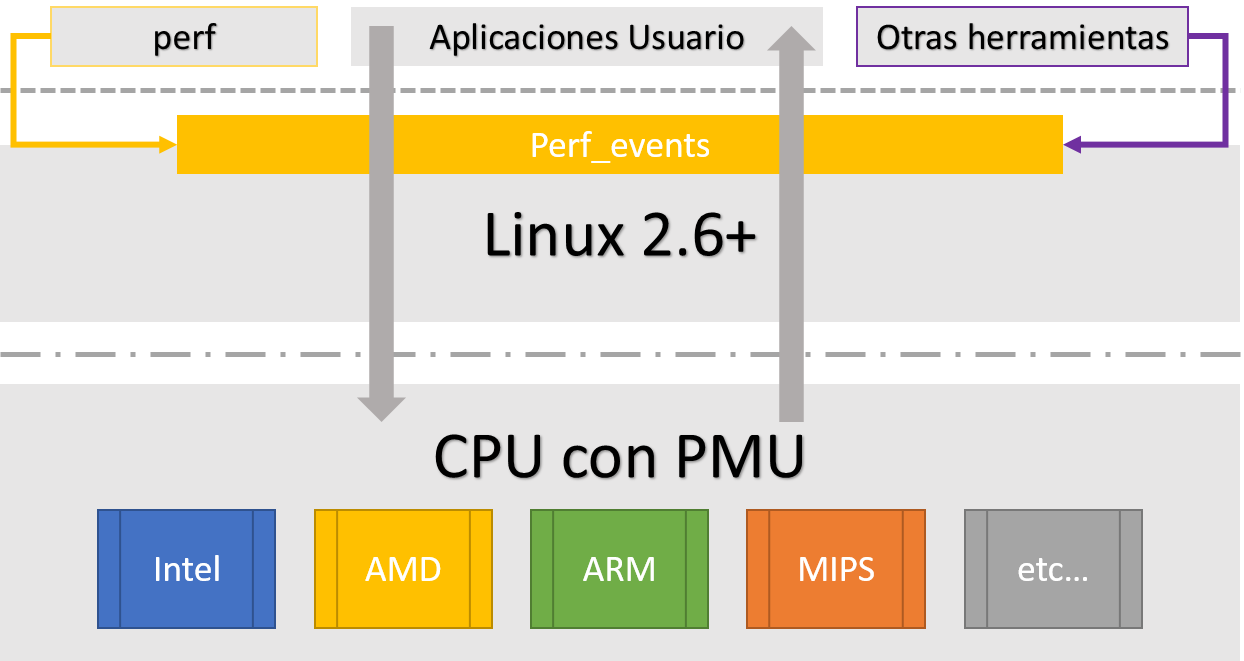
\includegraphics[scale=.45]{imagenes/perfArchitecture.png}
	\caption{Arquitectura de operación del framework provisto por \emph{Perf}.}
	\label{fig:perfFramework}
\end{figure}

Además de su gran capacidad para colectar datos, Perf es una herramienta de sencillo uso, pues su funcionamiento se basa en la supervisión de un determinado proceso o tarea de la cual construye un archivo con la información que se haya seleccionado a colectar \cite{article:perf}. Para ello, se pueden emplear las utilidades \verb=perf-record= y \verb=perf-stat= las que trabajan supervisando un determinado proceso y proveiendo paginas de datos al espacio del kernel que son rellenadas con información del sistema de dicho proceso y son retornadas al proceso responsable construyendo un informe a modo de output\footnote{La asignación del espacio de páginas a rellenar se hace por medio de la utilidad \verb=mmap= de Linux, que provee direcciones virtuales en un proceso para almacenar información.} (Ver figura \ref{fig:perfRecord}). Posteriormente, se pueden realizar operaciones de análisis más exhaustivo sobre dichos archivos de resultados.

El potencial de ésta herramienta la perfila como una utilidad indispensable para el estudio en cuestión. En primer lugar por su capacidad de análisis de ejecución de código que permite obtener información cuantificada de las llamadas a sistema y de la dinámica del árbol de llamados\footnote{Acá explicar brevemente que es un árbol de llamados} que permite reconocer la naturaleza de las funciones involucradas en el caso de estudio. En segunda instancia Perf es una estupenda herramienta para la recolección de datos de hardware al aprovechar el uso de la \emph{Performance Monitoring Unit (PMU)} del hardware del sistema, una característica que será revisada en detalle en secciones posteriores.

\begin{figure}[!h]
	\centering
	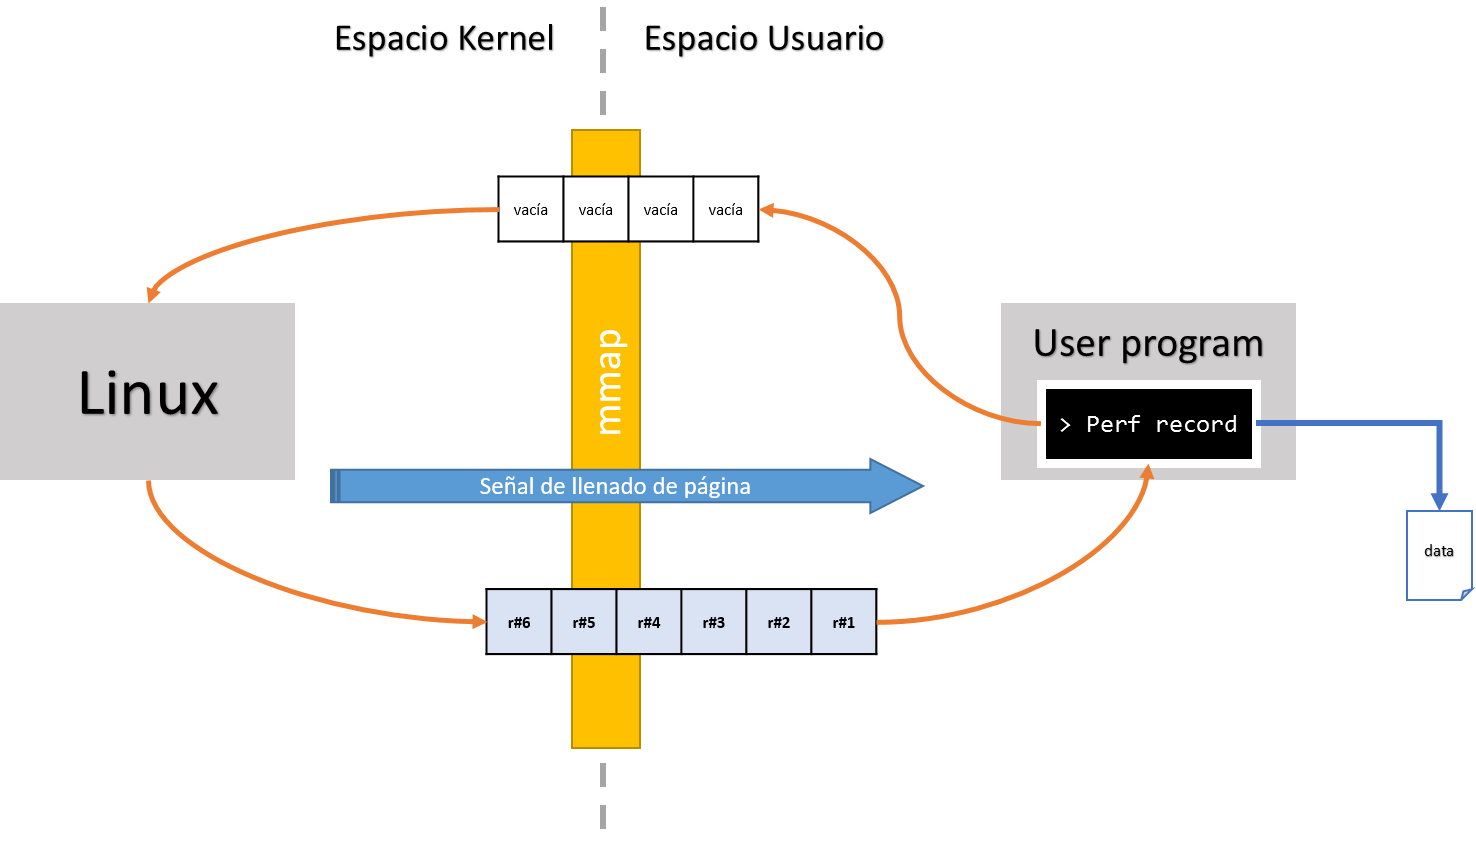
\includegraphics[scale=.45]{imagenes/perfRecord.png}
	\caption{Esquema de captura de datos de un programa usando el comando \emph{perf-record}.}
	\label{fig:perfRecord}
\end{figure}

\subsubsection{FTrace}
Ftrace\footnote{Mayor documentación disponible en \url{http://elinux.org/Ftrace}} es otra poderosa herramienta para estudios de profiling disponible para sistemas Linux \cite{paper:FTraceSony}. Su funcionamiento opera de naturaleza muy intima con respecto al kernel mismo pues su recolección de datos se basa en el rastreo de la ejecución de funciones de forma dinámica en el espacio de kernel, lo que lo hace una estupénda utilidad para el estudio de llamadas al sistema pudiendo recuperar datos como el tiempo de ejecución y cantidad de ocurrencia de las mismas.

Para su uso, FTrace opera como un verdadero framework del sistema sobre el kernel, del cual se pueden usar distintos métodos de rastreo de llamadas basados en distintos algoritmos. Una de las funciones más poderosas de FTrace es el resultado que se puede obtener por medio de la instrumentación de código, que se refiere a la práctica de incorporar a los programas a analizar \emph{tracepoints}, que son declaraciones explicitas de secciones de código a analizar y registrar. A pesar de que ésta característica es muy cómoda para programas propios, en el caso del análisis de funciones y llamadas de sistema la instrumentación de código es una característica obviable, siendo sólo necesaria la precisión de qué llamadas considerar en el análisis pues el sistema es flexible para hacer análisis directamente de funciones del sistema. El uso de ésta herramienta es muy flexible, siendo activable a disposición del usuario y conservando un registro de resultados. Además, FTrace es altamente configurable pudiendo explicitar filtros que usar como registros para las llamadas de sistema a analizar.

El provecho que se puede sacar de ésta herramienta es usar su capacidad para cuantificar tiempo de funciones del kernel para estudiar la atomicidad de las llamadas bloqueantes del sistema. Así por ejemplo, se pretende determinar el tiempo que se pasa en estados bloqueantes de spinlocks (que terminan siendo pasos de \emph{busy-waiting}) en los cuales sólo se pierde tiempo por caso de contención.

\subsection{Metodología de Experimentación}

Dado que la naturaleza de éste estudio se relaciona con el comportamiento de funciones del sistema que administran las primitivas de acceso y sincronización del Interet socket, se realizarán las configuraciones pertinentes para cada herramienta a fin de contemplar dichos puntos de análisis. En el caso de Perf, la recolección de datos clásica se realizará con la herramienta \verb=perf-record=, y se realiza un post-procesamiento sobre el archivo de reporte generado, para colectar los datos estadísticos asociados a las distintas funciones de manejo de spinlock antes mencionadas\footnote{Correspondiente a la ejecución del proyecto \url{https://github.com/sebablasko/Test_MultiThreadStressTransmision} con privilegios de administrador.}.

Por otro lado, para el estudio con FTrace la configuración resulta un poco más compleja. Dado que es una herramienta de traceo que opera inspeccionando las llamadas de funciones de sistema, la activación de FTrace sobrecarga el funcionamiento del sistema general. Por ello, FTrace se debe activar y desactivar manualmente para analizar sólo los instantes de operación de la prueba de interés. Además, dado el amplio espectro de funciones disponibles para inspeccionar con el framework, deben emplear las funciones de filtrado de funciones a tracear que provee el mismo framework. En pos de capturar funciones en línea con la diniámica del spinlock del Internet socket, se configuró FTrace para capturar estadísticas de todas aquellas funciones definidas anteriormente.

\begin{lstlisting}[style=BashInputStyle, label={code:ftrace}, caption={Configuración de filtros de FTrace sobre funciones a estudiar.}, captionpos=b]
[sebastian@labs-vhost ~]$ echo *spin* > /sys/kernel/debug/tracing/set_ftrace_filter 
[sebastian@labs-vhost ~]$ cat /sys/kernel/debug/tracing/set_ftrace_filter 
mutex_spin_on_owner
spin_msec
_spin_trylock
_spin_lock_irqsave
_spin_lock_irq
_spin_lock
_spin_unlock_irqrestore
_spin_lock_bh
_spin_trylock_bh
_spin_unlock_bh
bit_spin_lock
kvm_vcpu_on_spin
\end{lstlisting}

Por otra parte, el encendido y apagado del framework mismo se configuró como parte del programa de prueba\footnote{\url{https://github.com/sebablasko/Test_UDPTrace/}}. En el mismo se configuró la opción \verb=set_ftrace_pid= para explicitar la inspección de FTrace sólo para el script de prueba, además del uso de la utilidad \verb=trace_marker= para instrumentar porciones de código de la prueba (como creación de threads, y término de consumo de datos) que permitiese una mayor facilidad al momento de estudiar los logs de ejecución recuperados.

\subsection{Resultados}
Nos topamos con que las tendencias de tiempos son similares a las de los tiempos de esas llamadas, luego, hay una correlacion de esta estructura inhenrente al socket es la que causa el cuello de botella: indicio, el socket entero está siendo contenido por el spinlock de su estructura.

\subsubsection{Perf}
Gráfico de resultados de perf

\begin{figure}[!h]
	\centering
	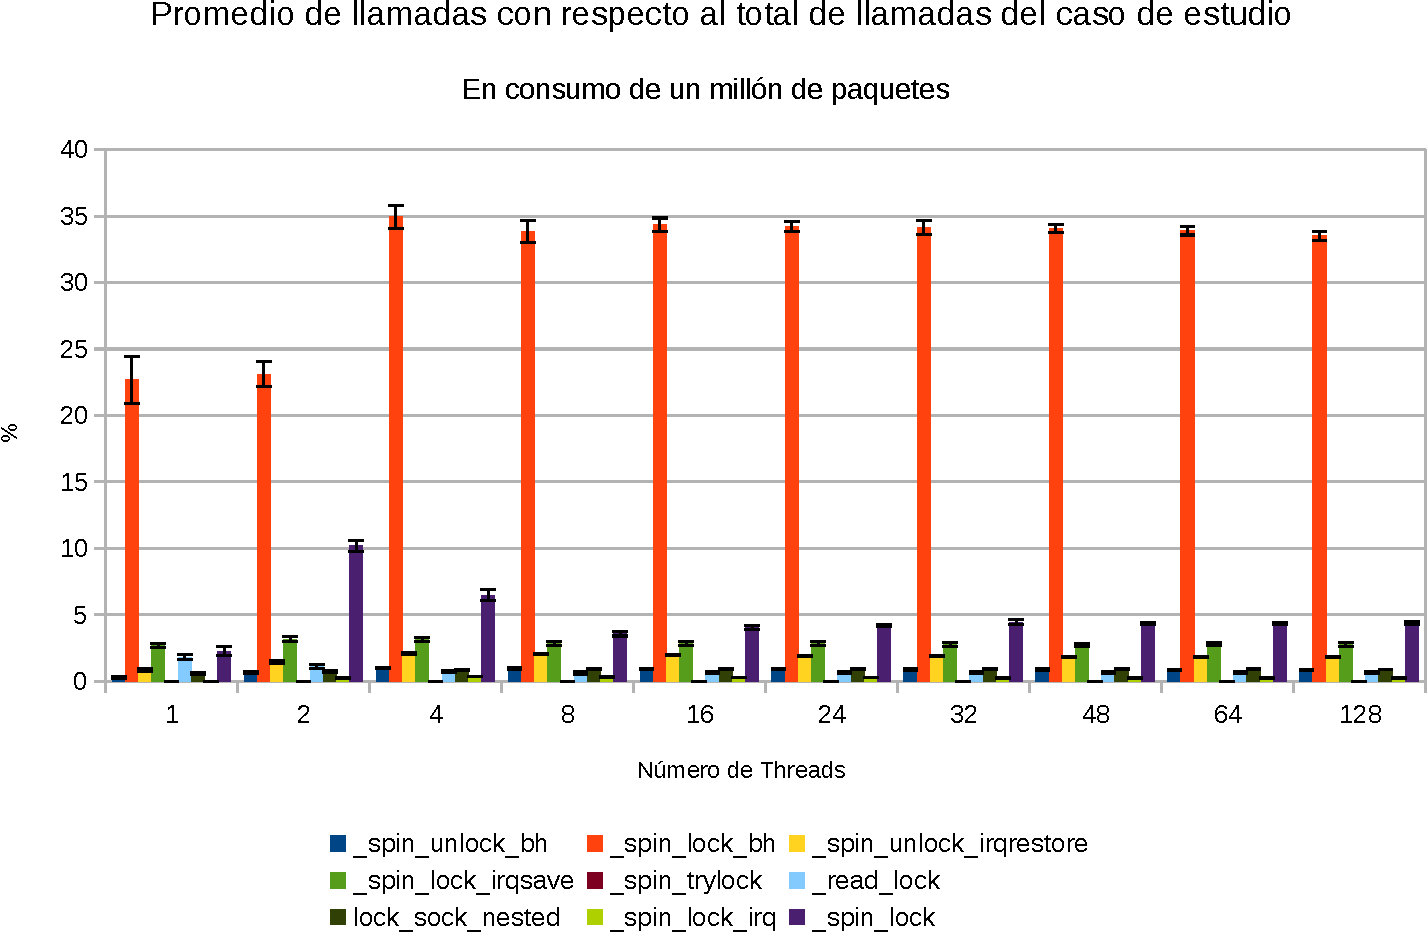
\includegraphics[scale=.5]{resultados/perfdetalle-crop.pdf}
	\caption{Resultados experimentales de los porcentajes de ejecución de las llamadas a sistema recolectadas por \emph{Perf}.}
	\label{fig:resPerf}
\end{figure}

Para reconocer mejor la dinámica de consumo de tiempos en las funciones inspeccionadas en el caso de estudio, se usaron los reportes generados por Perf para construir un nuevo tipo de visualización de llamadas a sistema: Un \emph{Call-Graph-Chart} (Ver imagen \ref{fig:rescallGraph}), de manera de poder reconocer los bloques de funciones más repetidos en la ejecución del caso de prueba. Para ésta visualziación se aporvechó el script \emph{gprof2dot}\footnote{\url{https://github.com/jrfonseca/gprof2dot}}.
\begin{figure}[!h]
	\centering
	
\includegraphics[scale=.5]{imagenes/fcfm}
	\caption{Visualización de call-graph identificando las llamadas a sistema y sus pesos en el caso de prueba.}
	\label{fig:detalleFtrace}
\end{figure}

\subsubsection{FTrace}
Gráfico de resultados de FTrace
\begin{figure}[!h]
	\centering
	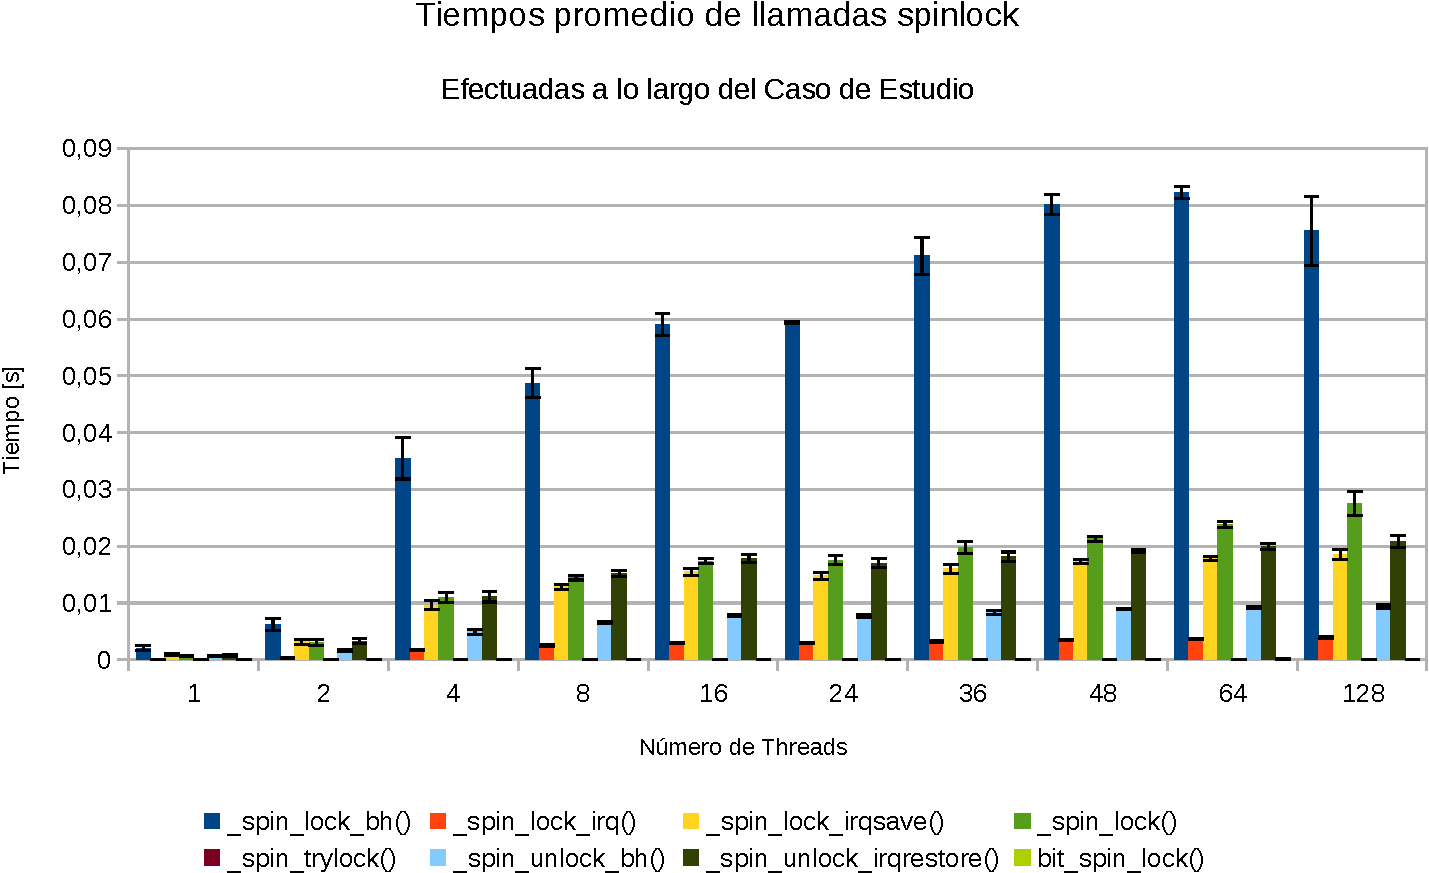
\includegraphics[scale=.5]{resultados/detalleFtrace-crop.pdf}
	\caption{Resultados experimentales de los tiempos de ejecución de las llamadas a sistema recolectadas por \emph{FTrace} para la adquisición y liberación del lock.}
	\label{fig:}
\end{figure}

Ahora hablar de los tiempos totales de bloqueo
\begin{figure}[!h]
	\centering
	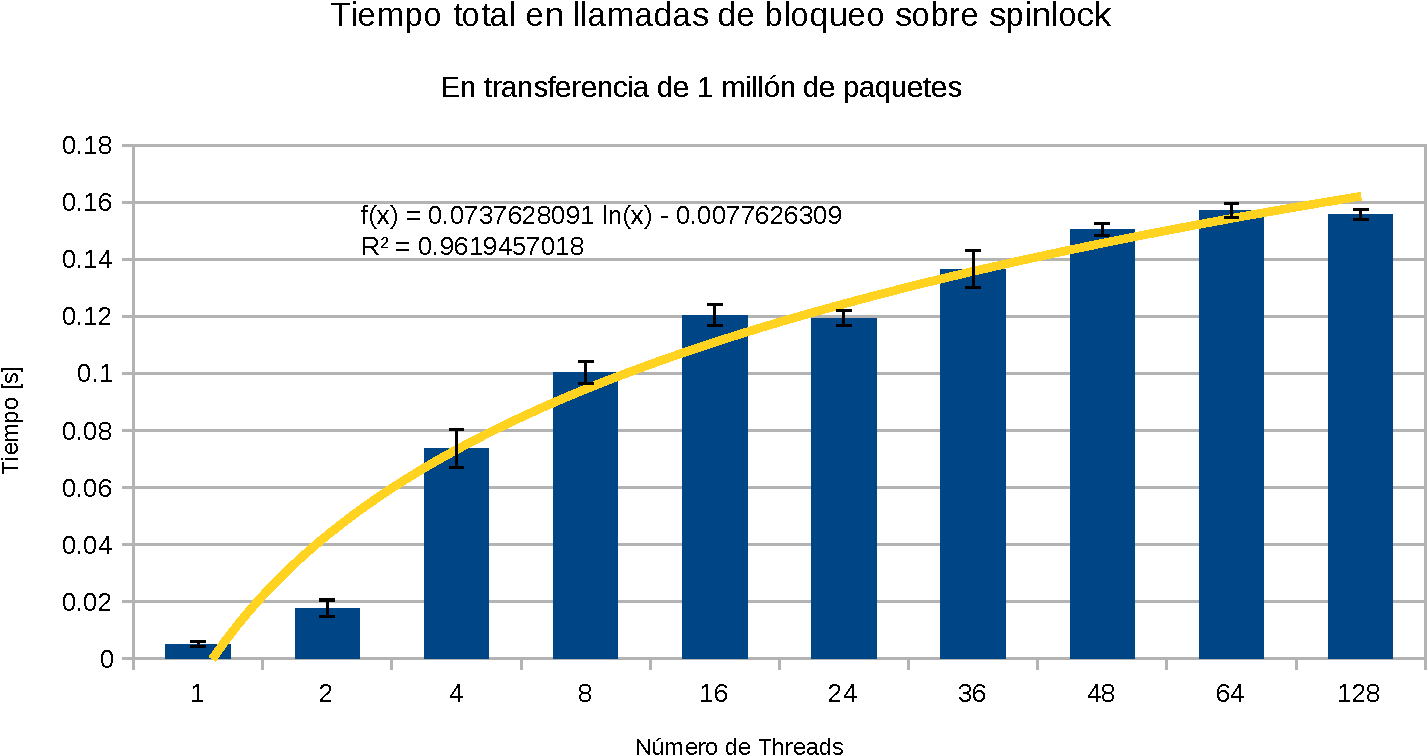
\includegraphics[scale=.5]{resultados/sumaFtrace-crop.pdf}
	\caption{Tiempos totales de bloqueo sobre el lock por las distintas llamadas de sistema capturadas por \emph{Ftrace} en el caso de estudio juntos con una curva de aproximación de tendencia.}
	\label{fig:sumaFtrace}
\end{figure}

Finalmente, si se revisan las tendencias separando las distintas operaciones de bloqueo y liberación del lock
\begin{figure}[h!]
	\centering
	\hspace*{\fill}
	\subfigure[Funciones de Bloqueo]{
		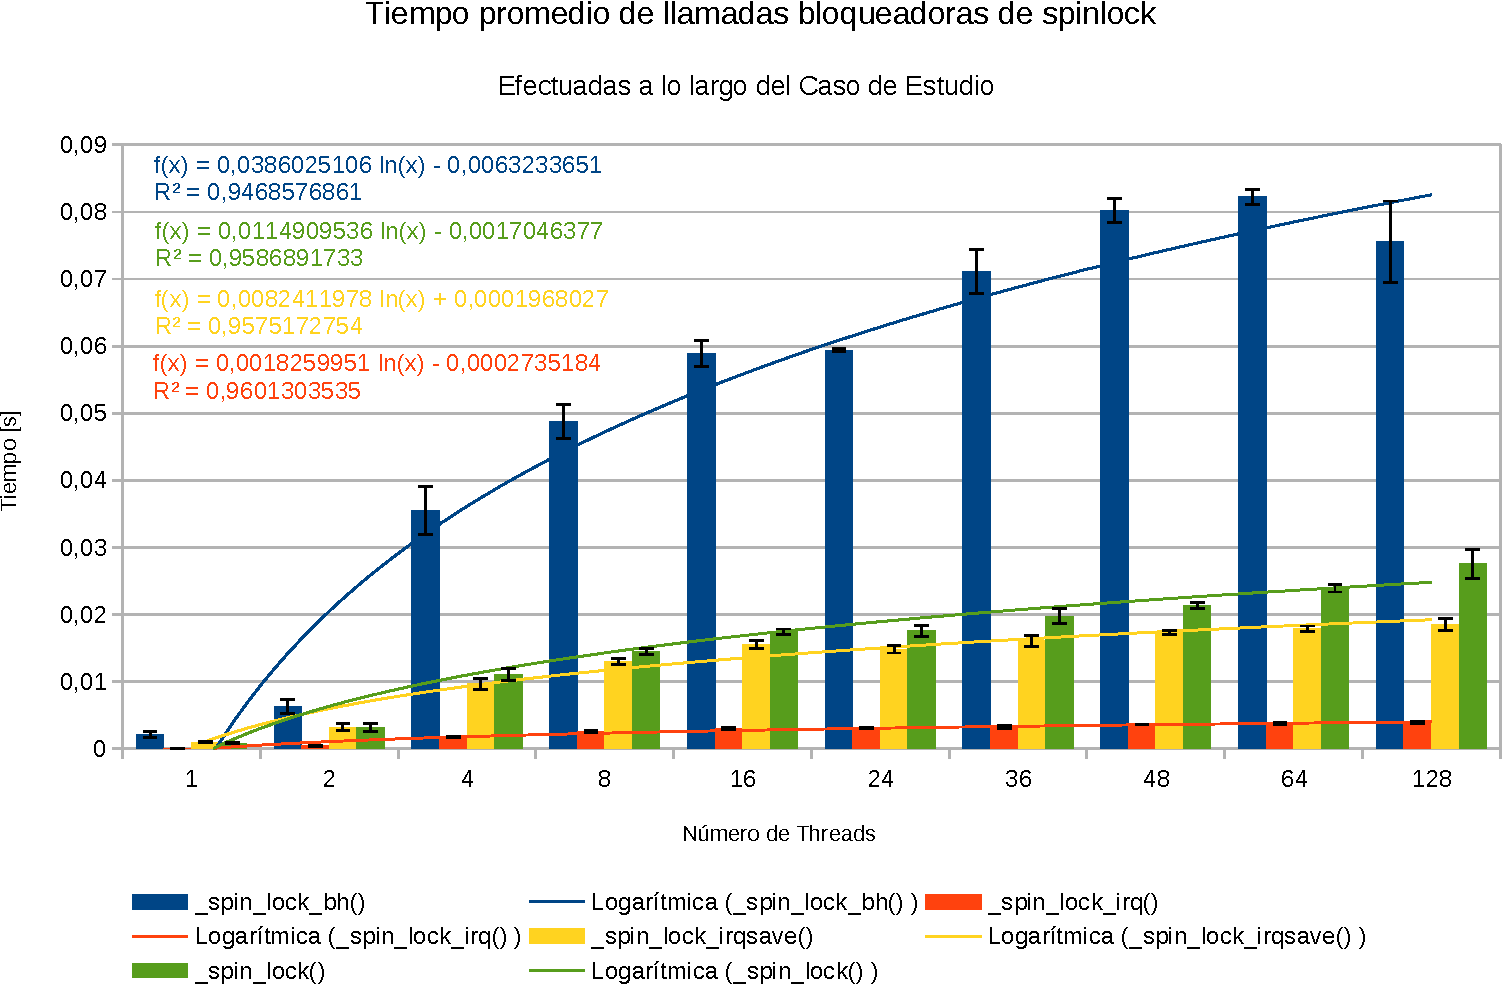
\includegraphics[width=.47\textwidth]{resultados/bloqueantesftrace-crop.pdf}
		\label{fig:ftracebloquea}
	}\hfill
	\subfigure[Funciones de Liberación]{
		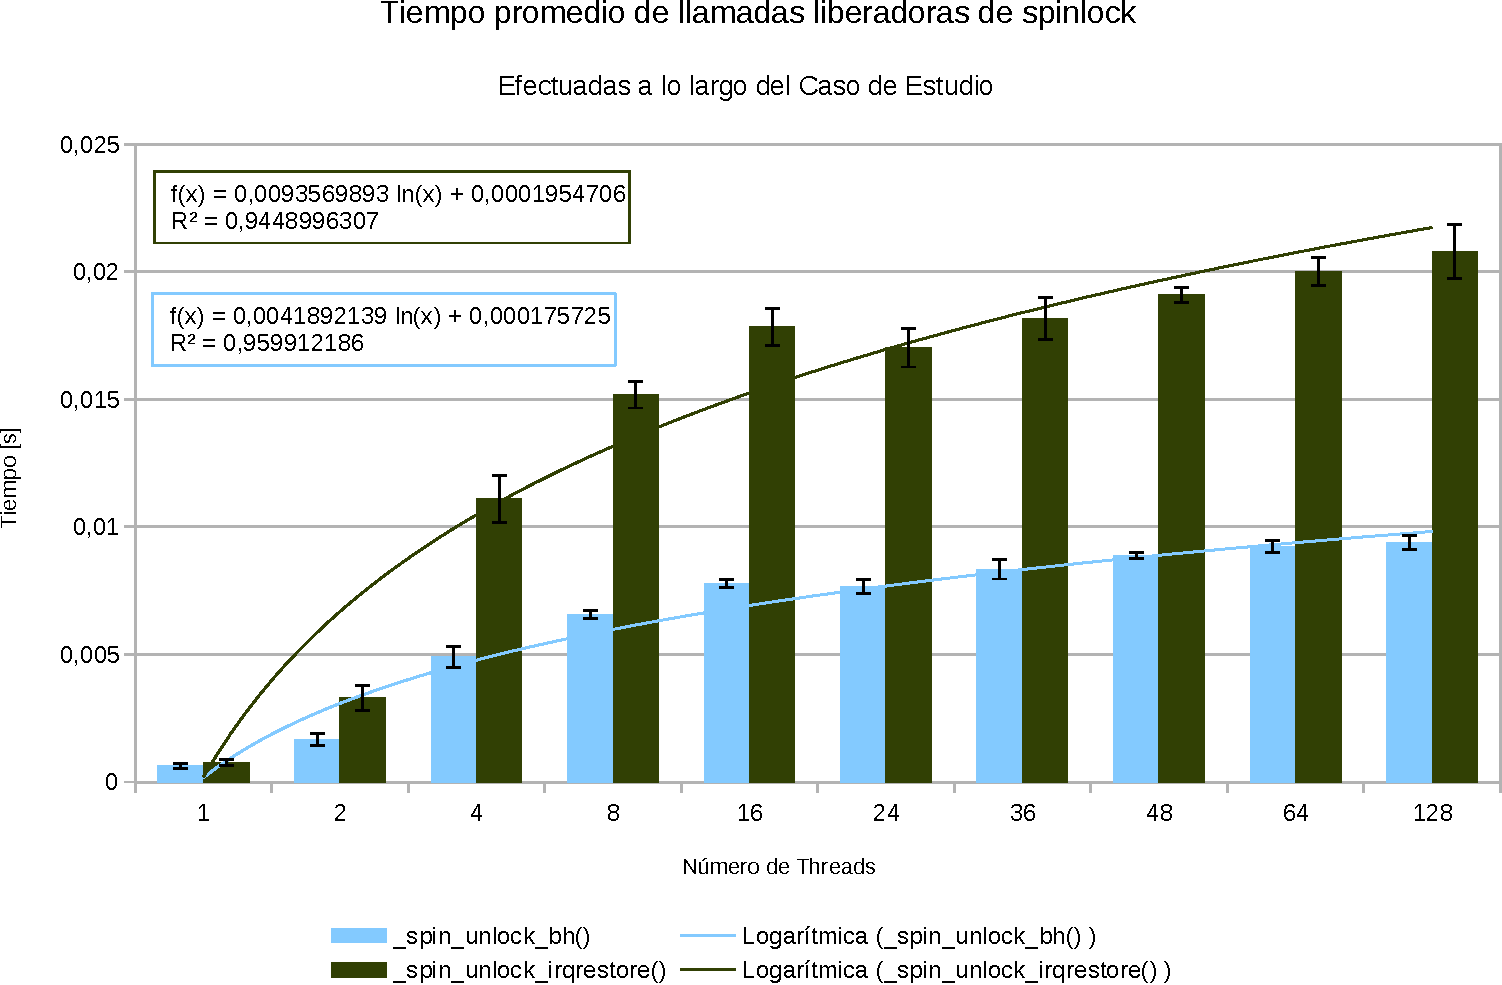
\includegraphics[width=.47\textwidth]{resultados/liberadorasFtrace-crop.pdf}
		\label{fig:ftracelibera}
	}
	\caption{Graficos con tendencias de tiempos del lock capturados con \emph{Ftrace} a lo largo del caso de estudio.}
	\label{fig:Ftracebloquealibera}
	\hspace*{\fill}
\end{figure}



\subsection{Análisis y Discusión de Resultados}
Aka un análisis general de los resultados en términis de gráficos obtenidos

\subsubsection{TraceDisplay}
Para poder obtener una interpretación adicional del fenómeno reconocido, se construyó una herramienta de visualziación de las llamadas a sistema para funciones de sincronización que permitiese reconocer las porciones de tiempo que tomasen en cada procesador dichas funciones. Para ello, la herramienta denominada \emph{TraceDisplay} recibe un log generado con \emph{FTrace} que incluya las llamadas de sistema yá filtradas, y construye un mapa de tiempo coloreado donde se pueden apreciar las porciones de tiempo que consume cada llamada y desde cual CPU se originan. El resultado se puede apreciar en la imagen \ref{fig:traceDisplay} donde se ilustra el caso de analizar [[AKA FALTA EXPLICAR EL CASO EVALUADO]].

Éste subproducto de la investigación principal junto con su documentación de uso está publicado\footnote{Disponible en \url{https://github.com/sebablasko/TraceDisplay}} y disponible para su uso.

\begin{figure}[!h]
	\centering
	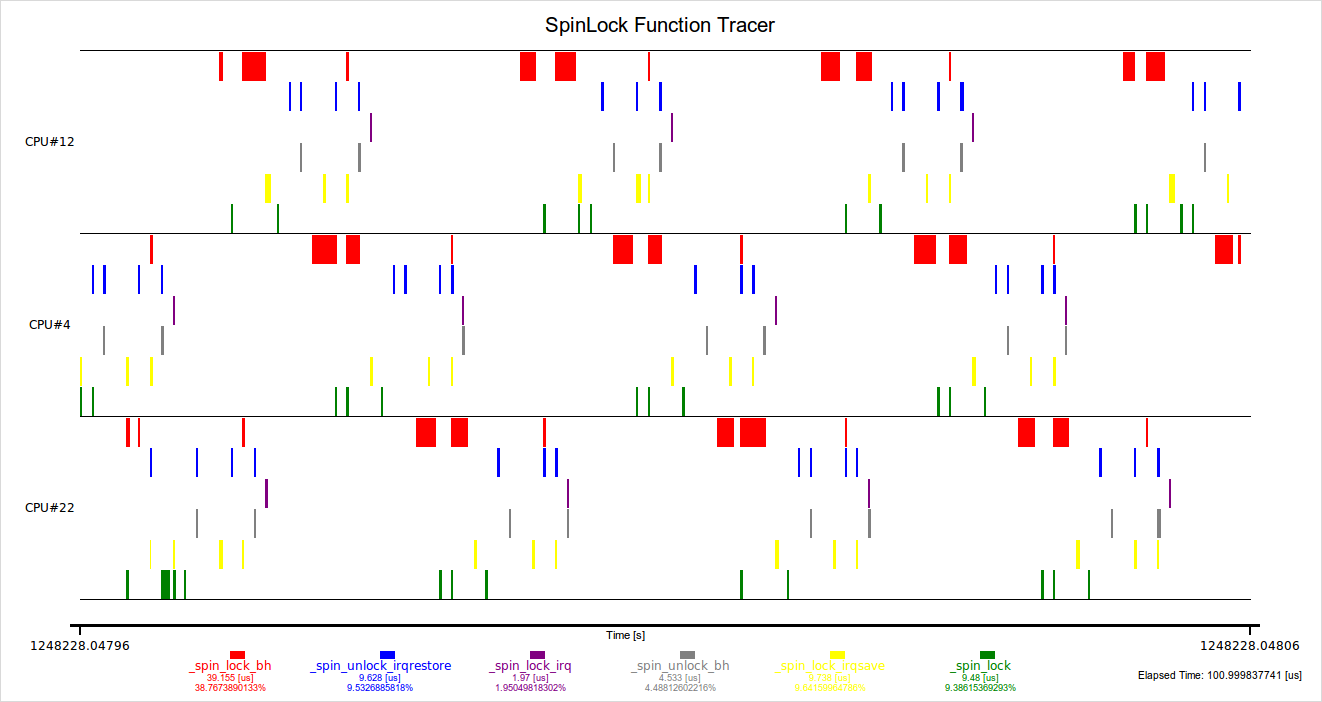
\includegraphics[scale=0.34]{imagenes/traceVisualization.png}
	\caption{Visualización de aplicación de llamadas de sistema de sincronización realizadas entre procesadores, generada con la herramienta TraceDisplay.}
	\label{fig:traceDisplay}
\end{figure}

Resultados como el mostrado en la figura \ref{fig:traceDisplay} ilustran como, en la práctica, las operaciones de bloqueo se terminan ejecutando serializadamente, aún cuando son distintos los CPU que los originen. Esto producto de que es una misma estructura la que se está compartiendo y así, se puede deducir un sobrecosto producido por dicha serialziación en el acceso.

\subsection{Conclusiones}
A raíz del estudio de operación de primitivas de sincronización del sistema se pueden rescatar varios aspectos interesantes:
\begin{itemize}
\item La tendencia en los costos de tiempo son crecientes a medida que se agregan hilos que consumen el mismo socket. Ello tanto en porcentaje de llamadas de sistema, como también en tiempos netos en esas llamdas.
\item Se identifican distintas estructuras bloqueantes para sincronización activas a lo largo del caso de estudio, sin embargo se destacan estructuras de tipo spinlock como las más reiteradas en el rastro de llamadas a sistema. Spinlock propio del mecanísmo de protección de la estructura socket accesada.
\item Se destaca una tendencia de naturaleza logaritmica en el crecmimiento de tiempos que toman las llamadas bloqueantes sobre el spinlock del socket, ajustada con un coeficiente de determinación superior al 90\%.
\end{itemize}
A raíz de lo anterior, se reconoce en el spinlock de protección del socket como un punto de cuello de botella al momento de emplear accesos concurrentes a una estructura socket. Ello al actuar como un punto de bloqueo que termina serializando el acceso al consumo de datos y que, lejos de reducir los tiempos paralelizando el acceso, los aumenta al serialziarlos y deber coordinar los hilos para ello.

\section{Estudio de Canales de Comunicación de Hardware}
La segunda hipótesis para explicar la mala performance del caso de estudio presentado se centra en una componente de hardware más que de software. Cómo ya se mencionó, la capacidad multiprocesador de que se dispone en equipos modernos no es un recurso fácil de aprovechar, de hecho requiere una sofisticada operación y diseño tanto de las aplicaciones que solicitarán recursos, como del sistema operativo que ha de administrarlos. Como se repasó en secciones anteriores, la capacidad de paralelísmo viene dada gracias a un conjunto de protocolos y algoritmos de muy bajo nivel que coordinan y mantienen en estado coherente las distintas componentes de datos para los diferentes procesadores \cite{paper:MESI, paper:snoop}, sin embargo, por muy sofisticados que dichos mecanismos sean, las nuevas tecnologías de hardware que prometen velocidades de trasnferencia y acceso nunca antes imaginiadas podrían significar un problema para éstas componentes, sobrepasándolos de cierta forma.

Es precisamente en ésta línea que se establece la segunda hipótesis. En éste caso, se adjudican las responsabilidades por el mal rendimiento presentado a un problema de contención de recursos (nuevamente al spinlock de los sockets), pero ésta vez relacionado a la persistencia en el acceso al mismo y a la disponibilidad que se da del mismo a través de los mecanismos antes mencionados. En las arquitecturas modernas, los protocolos \emph{MESI} y de \emph{SNOOP} son cruciales en la operación de ejecuciones paralelas para garantizar integridad en los datos, pero las arquitecturas modernas proponen nuevas distribuciones de los componentes internos de hardware, dotando de canales de comunicación de mayor velocidad de transmisión y reasignando los recursos físicos. Ésta hipótesis plantea la posibilidad de que el degradamiento del caso de estudio sea generado por un fenómeno de \emph{Caché Bouncing}.

\begin{defn}[ver \cite{paper:cachebouncing}] \textbf{Caché Bouncing} corresponde a un fenómeno producido en entornos multiprocesador, cuando distintas CPU realizan modificaciones a una linea de caché especifica que está siendo referenciada por varios procesadores. La modificación de la linea modificada se trasnfiere de caché en caché según los protocolos de consistencia del sistema. Éste fenómeno impone una significativa carga en el bus de memoria y los canales de comunicación afectados pudiendo degenerar en una degradación generalizada del sistema.
\end{defn}

En ésta línea, el fenómeno de \emph{Cache Bouncing} se podría manifestar dada la arquitectura del sistema, la que al contemplar bancos de memoria diversos, algunos compartidos y otros exclusivos para los núcleos de procesamiento, podría estar manifestandose como resultado de las modificaciones concurrentes de los distintos procesadores sobre la estructura socket compartida, y más precisamente sobre el spinlock del socket. Lo anterior combinado a la operación de los protocolos de consistencia y correctitud para las lineas de caché del sistema postulan evidencia que hace perfectamente posible el que se esté generando un overhead de comunicación que termine sobrecargando los tiempos totales de ejecución del caso de estudio.

Para validar la hipótesis anterior es preciso un cabal entendimiento de la arquitectura de hardware objetivo, a fin de poder localizar puntos de contención junto con una comprensión importante de la \emph{Performance Monitoring Unit} que provee el fabricante, lograr configurarla y aprovecharla para la recolección de datos finales. En las siguientes secciones se realiza un estudio de la arquitectura descrita en la figura \ref{fig:pc3} del equipo sobre el que se realizan las pruebas experimentales reales. Posteriormente se realiza un análisis experimental de las tendencias presentes en una tarea de acceso concurrente como la descrita en el caso de estudio de ésta investigación con el fin de corroborar o descartar las sospechas ya mencionadas del efecto de contención y \emph{caché bouncing} por eventos de perfomance de hardware.

\subsection{Características de Arquitecturas de Hardware Modernas}
Cómo ya se mencionó en secciones anteriores los fabricantes de partes y piezas de computadoras están constantemente desarrollando importantes avances, de la mano con el desarrollo técnico de piezas que brinda mejores componentes de hardware cada día. La linea de desarrollo de infraestructura de hardware principal de los computadores no está excenta de dicha evolución. En secciones anteriores se presentó como las arquitecturas han evolucionado desde el primer esquema \emph{SMP} propuesto con la distribución \emph{FSB}, pasando luego por nuevas configuraciones como \emph{DIB} y \emph{DHSI}, entre otras. Sin embargo, el desarrollo ha sido constante y hoy las arquitecturas han degenerado en esquemas bastante más complejos en pos de aprovechar al máximo la capacidad de los procesadores en la línea del paralelísmo.

\subsubsection{Arquitectura Intel QuickPath}
Al año 2008, el fabricante de procesadores Intel® lanzó al mercado una nueva tecnología denominada \emph{Intel QuickPath Architecture} \cite{paper:quickpath} la que platea un nuevo esquema organizacional de los componentes internos de la placa principal de las computadoras, así como también un nuevo esquema de conectividad entre los componentes de la misma, prometiendo entre otras cosas: Un sistema más confiable, eficiente, rápido y escalable, que podría aprovechar mejor la capacidad de los múltiples procesadores de su misma linea. La apuesta de Intel resultó todo un éxito. Rápidamente \emph{QuickPath} se posicionó en el mercado para competir con la tecnología \emph{HyperTransport} desarrollada por \emph{AMD}\footnote{AMD es el principal competidor de Intel en la industria de la manufactura de microprocesadores. \url{http://www.gestiopolis.com/intel-vs-amd-guerra-procesador/}}, abriendo paso definitivamente a una era, dejando atras el enfoque \emph{FSB}.

\begin{figure}[!h]
	\centering
	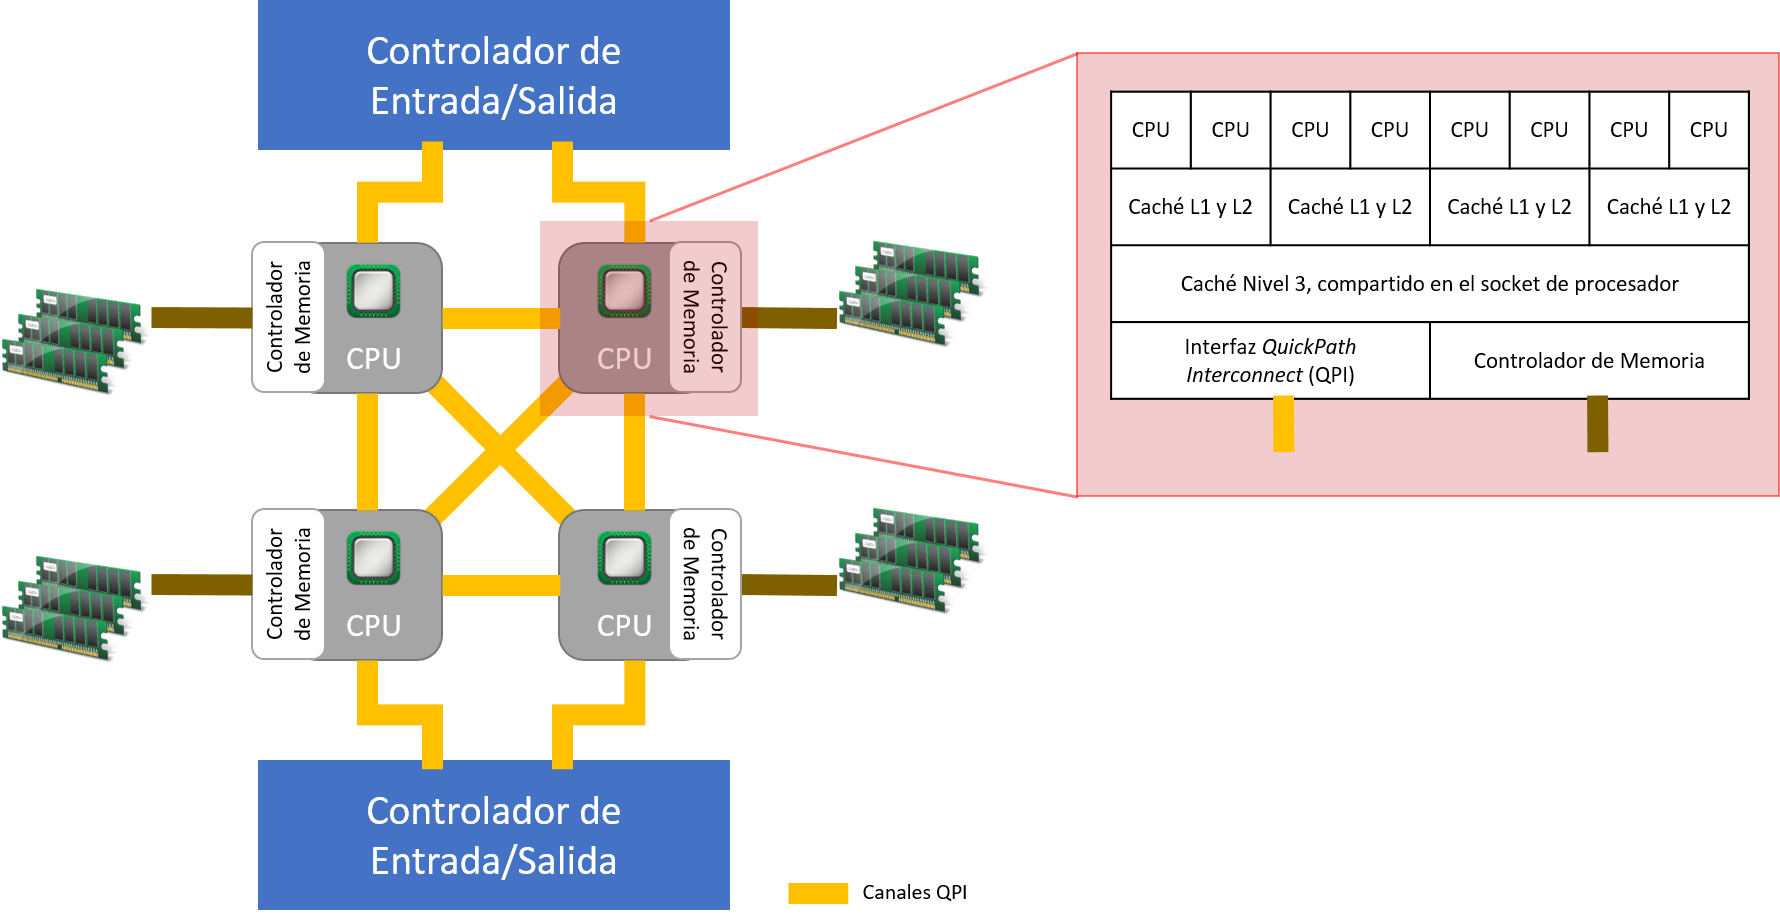
\includegraphics[scale=.5]{imagenes/quickpath2.png}
	\caption{Diseño organizacional de los componentes de sistema en una arquitectura estándar \emph{QuickPath} de Intel.}
	\label{fig:quickpath}
\end{figure}

El esquema \emph{QuickPath} postula una reformación arquitectural de los componentes principales de un sistema \ref{fig:quickpath}. En éste esquema, las distintas unidades de procesamiento (CPU) están interconectadas por canales de comunicación especiales denominados \emph{Intel QuickPath Interconnect - QPI} que son conexiones punto a punto entre CPU de enorme velocidad de transferencia (llegando hasta 25 GB/s), los que junto con modificaciones al tradicional protocolo MESI, flexibiliza los protocolos de coherencia de caché dotando así de mayor eficiencia y velocidad de acción entre procesadores al ser una comunicación directa.
Por otro lado, en \emph{QuickPath} cada CPU dispone de su propio controlador de memoria y de un banco de memoria de acceso próximo. Dicho diseño se denomina un nodo \textbf{NUMA} de sus siglas en inglés \emph{\textbf{N}on \textbf{U}niform \textbf{M}emory \textbf{A}ccess} [CITA A NUMA] la que permite a las CPU de cada nodo NUMA disponer de un banco de memoria con un acceso garantizado más rápido que al que se tendría acceso en una arquitectura tradicional. El enfoque \emph{NUMA} se aprovecha del principio de localidad de memoria \cite{paper:memorylocality}, por la cual postula que los datos son separables en su acceso por las distintas CPU, logrando así mayor velocidad en el acceso a la memoria, y menor problemas de coherencia de la misma por modificaciones entre CPUs.

El diseño de Intel va más allá. Concientes de la necesidad de herramientas y utilidades para analizar la verdadera perfomance que provee ésta arquitectura, Intel provee unidades de monitoreo de perfomance (o \textbf{PMU}, por sus siglas en ingles \emph{\textbf{P}erformance} \textbf{M}onitoring \textbf{U}nit) que son componentes de hardware incorporado a los sistemas que permiten operaciones de inspección a nivel de comunicación entre componentes del sistema. A éste tipo de análisis se denomínan \emph{Estudios de Perfomance Counters}, dado que para poder realizar una medición, el fabricante de la PMU provee una colección de posibles eventos a colectar, con significaciones puntuales cada uno.

\begin{defn}[ver \cite{KAR00}] \textbf{Performance Counters} son identificadores de maquina que permiten cuantificar determinados eventos a nivel de hardware, como lecturas de caché, corrección de lineas de caché, comunicación de protocolos de coherencia, etc. Usados para analizar el comportamiento de ciertas unidades de hardware y que conforman la base de las herramientas de profiling para el rastreo en el comportamiento de funciones de un sistema.
\end{defn}
 
QPI imple,enta la wea de 5 capas!!!!! importante ponerlo!

El estudio de performance counters corresponde a uno de los estudios de más bajo nivel realizables en pos de obtener datos que representen la forma objetiva la comunicación entre componentes del sistema. Ello lo hace también un estudio dificultoso de realizar pues amerita un gran conocimiento de la arquitectura puntual sobre el sistema que se desea estudiar.

\subsection{Especificación y Captura de Eventos}
Para definir el marco conceptual de la prueba, se debe mantener presente el contexto de la hipótesis que fundamenta la misma. En éste caso, la motivación de éste estudio está en linea con entender el comportamiento de un comsumo concurrente en una estructura socket, o más precisamente, ver cómo una instancia de una primitiva de sincronización --un spinlock en este caso-- se comporta en un escenario multithread, dado que la misma podría alocarse en caches de distintos procesadores. En ese escenario, se busca estudiar cómo se manifestaría la expresión de los protocolos de coherencia de cache bajo circunstancias de ejecución en un escenario mutiprocesador que podrian dar cuenta de que el mal desempeño general del caso de estudio tiene sus origines en los mismos sistemas de coordinación de bajo nivel del sistema.

\subsubsection{Arquitectura de la máquina para las pruebas}
Siguiendo el caso de prueba evaluado a lo largo de la investigación, se inspeccionará el caso de estudio de saturación de un socket UDP en el equipo servidor multicore para pruebas (Ver fig. \ref{fig:hwspecs}). En éste caso, se cuenta con un equipo placa Dell Inc. 00NH4P A07, provisto de dos CPU Intel Xeon 5600 2.8Ghz, dotado de 6 cores cada uno. Cada CPU dispone de hasta tres niveles de cache de 192 kb, 1536kb y 12288kb respectivamente, que combinados con tres memorias de 4096MB (DDR3 1333MHz) cada uno, conforman 2 nodos NUMA, con un monto total de 24GB de memoria. Una configuración que es precisamente de la familia \emph{Intel QuickPath Architecture} y es enfocada a servidores multicpu \cite{report:intelxeon5600, manual:intelxeon5600}.

\begin{figure}[!h]
	\centering
	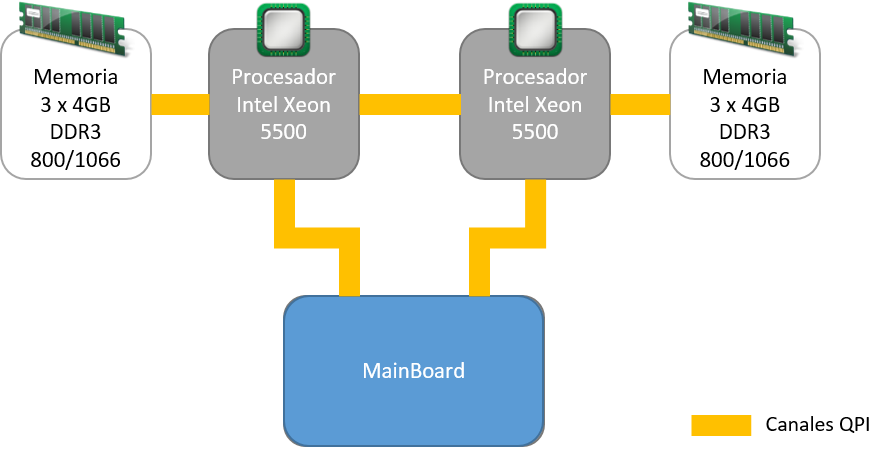
\includegraphics[scale=.7]{imagenes/arch24Cores.png}
	\caption{Esquema de arquitectura interna del esquipo servidor multicore sobre el que se realizan las pruebas de performance counters.}
	\label{fig:hwspecs}
\end{figure}

Al inspeccionar el sistema donde se evalúan las pruebas en detalle, se da cuenta de que para el modelo de procesador presente se dispone de 5 unidades de PMU disponibles, separables en 3 grupos (Ver código \ref{code:pmuavailable}):
\begin{description}
\item[PMU Genéricas] Incluyen a \verb=perf= y  \verb=perf_raw=. Disponen de las especificaciones estándar de perfomrance counters de la línea del software \emph{Perf}, lo cual las hace poco exactas en los valores descritos por cada evento y no necesariamente fieles a su descripción pues dependen en gran parte de que el fabricante sea riguroso en su implementación.
\item[PMU x86] PMU generacional de Intel para la línea x86 de Intel que incluye a \verb=ix86arch=. Dispone de eventos comunes a dicha linea de procesadores por lo que no da soporte especifico para la arquitectura \emph{quickPath} y del comportamiento multiprocesador.
\item[PMU westmere] PMU especificas de la línea Westmere [AKA UNA CITA] que soporta la base del desarrollo de la \emph{Intel QuickPath Architecture}, incluyendo a \verb=wsm_dp= y \verb=wsm_unc=. Es el nivel más exacto de PMU que provee el fabricante con los eventos más especificos y documentados del sistema.
\end{description}

\begin{lstlisting}[style=BashInputStyle, label={code:pmuavailable}, caption={Listado de \emph{PMUs} disponibles en el sistema, recuperado con la herramienta \emph{libpfm4}.}, captionpos=b]
	Detected PMU models:
[18, ix86arch, "Intel X86 architectural PMU", 6 events, 1 max encoding, 7 counters, core PMU]
[51, perf, "perf_events generic PMU", 104 events, 1 max encoding, 0 counters, OS generic PMU]
[53, wsm_dp, "Intel Westmere DP", 91 events, 2 max encoding, 7 counters, core PMU]
[54, wsm_unc, "Intel Westmere uncore", 52 events, 1 max encoding, 9 counters, uncore PMU]
[114, perf_raw, "perf_events raw PMU", 1 events, 1 max encoding, 0 counters, OS generic PMU]
\end{lstlisting}

\subsubsection{Metodología de captura de eventos}
Para la especificación de la captura de eventos, lo primero es prestar especial atención a la arquitectura interna en la comunicación interprocesador del sistema. En la figura \ref{fig:hwcomm} se da cuenta de los canales de comunicación que dispone el sistema estudiado.

\begin{figure}[!h]
	\centering
	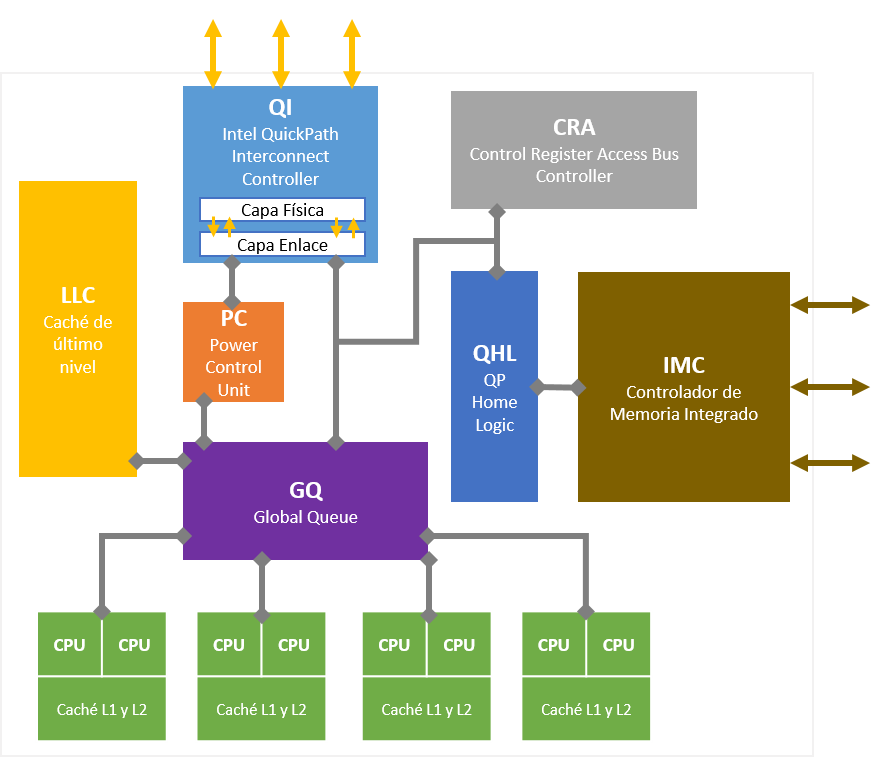
\includegraphics[scale=.8]{imagenes/QuickPathChannels.png}
	\caption{Esquema de arquitectura interna del equipo servidor multicore estudiado, ilustrando las vías de comunicación del procesador que da cuenta de los principales puntos de alta comunicación en el escenario de \textit{cache bouncing} por contención de valores.}
	\label{fig:hwcomm}
\end{figure}

La figura \ref{fig:hwcomm} da cuenta de los puntos en que se pueden suceder escenarios de congestión dados ya sea por un alto nivel de uso de los protocolos de coordinación de memoria o por un alto tráfico de comunicación entre CPUs. Dichos canales de comunicación podemos resumirlos en las siguientes funciones dedicadas de la arquitectura estudiada, que a su vez están asociadas a ciertos Performance Counters del sistema:

\begin{itemize}
\item Uso de los canales \emph{Intel QuickPath QPI}
\item Acciones del protocolo \emph{SNOOP}
\item Pasos de datos entre distintos caché y memoria
\item Transiciones del protocolo \emph{MESI(F)}
\end{itemize}


Con ello en mente, se consultó el manual oficial del fabricante \cite{manual:bigbigevents} en búsqueda de documentación acerca de eventos disponible en el sistema que se relacionaran a las operaciones antes descritas. De dicha documentación, combinado con la utilidad \emph{libpfm4}\footnote{Corresponde a una utilidad confeccionada para recuperar información sobre los código de inspección de eventos de performance counters de un sistema.}\footnote{\url{http://www.bnikolic.co.uk/blog/hpc-prof-events.html}} para la recolección de eventos disponibles en el sistema se colectaron un total de 143 eventos, cada uno con hasta 6 variantes de configuración, dando en total casi 500 posibles eventos a estudiar. En este escenario es preciso acotar los eventos a considerar de acuerdo a los 4 criterios antes descritos.


[[[Hablar un poco de dicha busqueda y del manual]]]]

Finalmente, siguiendo los 4 criterios de puntos problemáticos a estudiar se construyó una selección de eventos a considerar resumida en la tabla \ref{table:eventos}. Los eventos están divididos en dos grupos: \textbf{QPI/GQ/Cache} para eventos relacionados con movimiento o traslación de datos entre distintas estructuras de hardware, y \textbf{LinkLayer} para eventos referidos a protocolos de consistencia y sincronización que son pertinenetes a la capa de corrección en el esquema de capas del \emph{Quickpath}.

\begin{table}[h!]
\centering
\begin{tabular}{l|l}
\multicolumn{1}{c|}{{\bf QPI/GQ/CACHE}} & \multicolumn{1}{c}{{\bf LinkLayer}} \\ \hline
{ UNC\_GQ\_DATA\_FROM} & SNOOPQ\_REQUESTS \\
{ UNC\_GQ\_DATA\_TO} & SNOOPQ\_REQUESTS\_OUTSTANDING \\
{ UNC\_QHL\_REQUESTS} & SNOOP\_RESPONSE \\
{ L1D} & UNC\_QPI\_RX\_NO\_PPT\_CREDIT \\
{ L2\_DATA\_RQSTS} & UNC\_QPI\_TX\_STALLED\_MULTI\_FLIT \\
{ UNC\_LLC\_HITS} & UNC\_QPI\_TX\_STALLED\_SINGLE\_FLIT \\
{ UNC\_LLC\_MISS} & UNC\_SNP\_RESP\_TO\_LOCAL\_HOME \\
{ UNC\_LLC\_LINES\_IN} & UNC\_SNP\_RESP\_TO\_REMOTE\_HOME \\
{ UNC\_LLC\_LINES\_OUT} & UNC\_IMC\_RETRY
\end{tabular}
\caption{Total de eventos inspeccionados y estudiados en el caso de estudio de consumo concurrente sobre sockets UDP.}
\label{table:eventos}
\end{table}

Con los eventos a colectar más claros, se confeccionó una utilidad para la obtención de los códigos de registros de cada evento de interés. Utilidad que operando en conjunto con \emph{libpfm4} es capaz de parsear datos del sistema para generar una colección de eventos (ver Tabla \ref{table:codigoseventos}) en formato \verb=JSON=\footnote{\url{https://github.com/sebablasko/libpfm4PerformanceEventParser}}. según los cuales se debería tener una correcta representación del nivel de saturación y uso de los componentes.

Con el \verb=JSON= generado, se pueden hacer mediciones de forma sencilla usando la herramienta \verb=stat= de \emph{Perf} para generar un reporte de la cantidad de veces que se registre actividad en el evento estudiado, especificado en la misma herramienta.

\begin{lstlisting}[style=BashInputStyle, breaklines=true, captionpos=b, caption={Ejemplo de uso de Perf para colectar datos de una colección de eventos sobre un script llamado programa. En éste caso se configura para colectar datos de 2 eventos y dejar el reporte de salida en un archivo resultado.txt}]
	# perf stat -e r53003c,r5300c0 -o resultado.txt -- ./programa
\end{lstlisting}

Finalmente, de los output de Perf, se pueden estudiar los resultados finales de la comunicación efectiva generada a lo largo de la prueba.

\begin{table}[]
\centering
\begin{tabular}{|l|l|p{0.58\linewidth}|}
\hline
Nivel de Inspección                 & Registro & Descripción                                                \\ \hline
\multirow{8}{*}{Uso de QPI}         & r500104  & Cycles GQ data is imported from Quickpath interface        \\ \cline{2-3} 
                                    & r500204  & Cycles GQ data is imported from Quickpath memory interface \\ \cline{2-3} 
                                    & r500404  & Cycles GQ data is imported from LLC                        \\ \cline{2-3} 
                                    & r500105  & Cycles GQ data sent to the QPI or QMC                      \\ \cline{2-3} 
                                    & r500205  & Cycles GQ data sent to LLC                                 \\ \cline{2-3} 
                                    & r500405  & Cycles GQ data sent to cores                               \\ \cline{2-3} 
                                    & r500420  & Quickpath Home Logic remote read requests                  \\ \cline{2-3} 
                                    & r500820  & Quickpath Home Logic remote write requests                 \\ \hline
\multirow{3}{*}{Snoop}              & r530451  & L1D cache lines replaced in M state                        \\ \cline{2-3} 
                                    & r530251  & L1D cache lines allocated in the M state                   \\ \cline{2-3} 
                                    & r530851  & L1D snoop eviction of cache lines in M state               \\ \hline
\multirow{15}{*}{Pasos entre Cache} & r500108  & Number of LLC read hits                                    \\ \cline{2-3} 
                                    & r500208  & Number of LLC write hits                                   \\ \cline{2-3} 
                                    & r500109  & Number of LLC read misses                                  \\ \cline{2-3} 
                                    & r500209  & Number of LLC write misses                                 \\ \cline{2-3} 
                                    & r50010a  & LLC lines allocated in M state                             \\ \cline{2-3} 
                                    & r50020a  & LLC lines allocated in E state                             \\ \cline{2-3} 
                                    & r50040a  & LLC lines allocated in S state                             \\ \cline{2-3} 
                                    & r50080a  & LLC lines allocated in F state                             \\ \cline{2-3} 
                                    & r500f0a  & LLC lines allocated                                        \\ \cline{2-3} 
                                    & r50010b  & LLC lines victimized in M state                            \\ \cline{2-3} 
                                    & r50020b  & LLC lines victimized in E state                            \\ \cline{2-3} 
                                    & r50040b  & LLC lines victimized in S state                            \\ \cline{2-3} 
                                    & r50080b  & LLC lines victimized in I state                            \\ \cline{2-3} 
                                    & r50100b  & LLC lines victimized in F state                            \\ \cline{2-3} 
                                    & r501f0b  & LLC lines victimized                                       \\ \hline
\multirow{4}{*}{MESI}               & r501f0b  & L2 data demand loads in E state                            \\ \cline{2-3} 
                                    & r530126  & L2 data demand loads in I state (misses)                   \\ \cline{2-3} 
                                    & r530326  & L2 data demand loads in M state                            \\ \cline{2-3} 
                                    & r530526  & L2 data demand loads in S state                            \\ \hline
\end{tabular}
\caption{Colección de eventos resumidos para la inspección de los canales de comunicación del sistema en escenarios multithread.}
\label{table:codigoseventos}
\end{table}

Para poder comprender mejor las tendencias de comportamiento de los distintos eventos en cada instancia de prueba con una determinada configuración de threads, se evaluaron 3 escenarios de consumo para visualizar sus resultados\footnote{AKA URL AL REPO QUE TIENE ESTA PRUEBA DE PERFCOUNTERS}:
\begin{enumerate}
\item Lectura concurrente desde un dispositivo virtual como \verb=dev_null=.
\item Lectura exclusiva desde un socket UDP.
\item Lectura concurrente desde un socket UDP.
\end{enumerate}

De esta manera, se busca tener un punto de comparación de qué fenómeno se manifiesta en escenarios de lectura concurrente sobre un socket que no se manifiesta en otros escenarios.

\subsection{Metodología de Experimentación}
Hablar de que se empleará el caso de estudiode la siguiente manera blablabla, haciendo enfasis en que la captura de eventos se hace a través del software perf y que se evalúan distintas configuraciones de threads, repitiendo el experimento una cantidad X de veces.
\begin{equation}
T_i = \left\{ T_{i,1},T_{i,2},T_{i,3}, \dots ,T_{i,59}, T_{i,60}\right\} 
\end{equation}

Finalmente, se construye con cada evento un set de registros que guardan un valor promedio para una evaluación de ciertos threads.

\begin{equation}
Event_j = \left(\overline{T_{1}}, \overline{T_{2}}, \overline{T_{4}}, \overline{T_{6}}, \overline{T_{8}}, \overline{T_{16}}, \overline{T_{24}}, \overline{T_{36}}, \overline{T_{48}}, \overline{T_{60}}\right)
\end{equation}

\subsection{Resultados}
AKA mostrar que se reconocen dos tendencias entre los grupos de eventos (sobre el caso de udp concurrente).


\subsubsection{Correlación de Eventos}
Para poder comprender mejor la tendencia de comportamiento en el experimento entre los distintos eventos capturados se repasaron posibles mecanismos de visualziación que permitieran una simple comparación entre dichas mediciones. Se optó por emplear una visualziación mediante el uso de una matriz de correlación\footnote{\url{https://en.wikipedia.org/wiki/Correlation_and_dependence#Correlation_matrices}}, de manera de poder detectar facilmente conjuntos de eventos relacionados, ello combinando algúna estratégia de clusterización en el proceso de visualizar los datos. Ésta técnica es muy práctica y se ha empleado en otros escenarios sobre el mismo kernel en otras investigaciones con buenos resultados \cite{paper:clusteringKernel}.

\begin{figure}[h!]
	\centering
	\hspace*{\fill}
	\subfigure[]{
		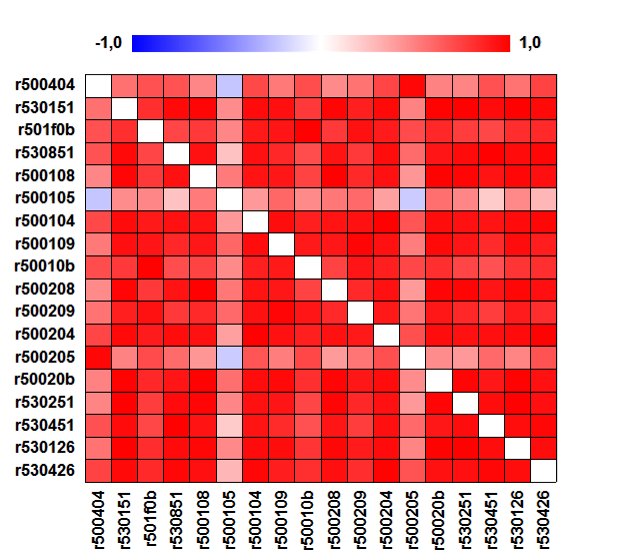
\includegraphics[width=.45\textwidth]{imagenes/corrgram0.png}
		\label{fig:corrgram:a}
	}\hfill
	\subfigure[]{
		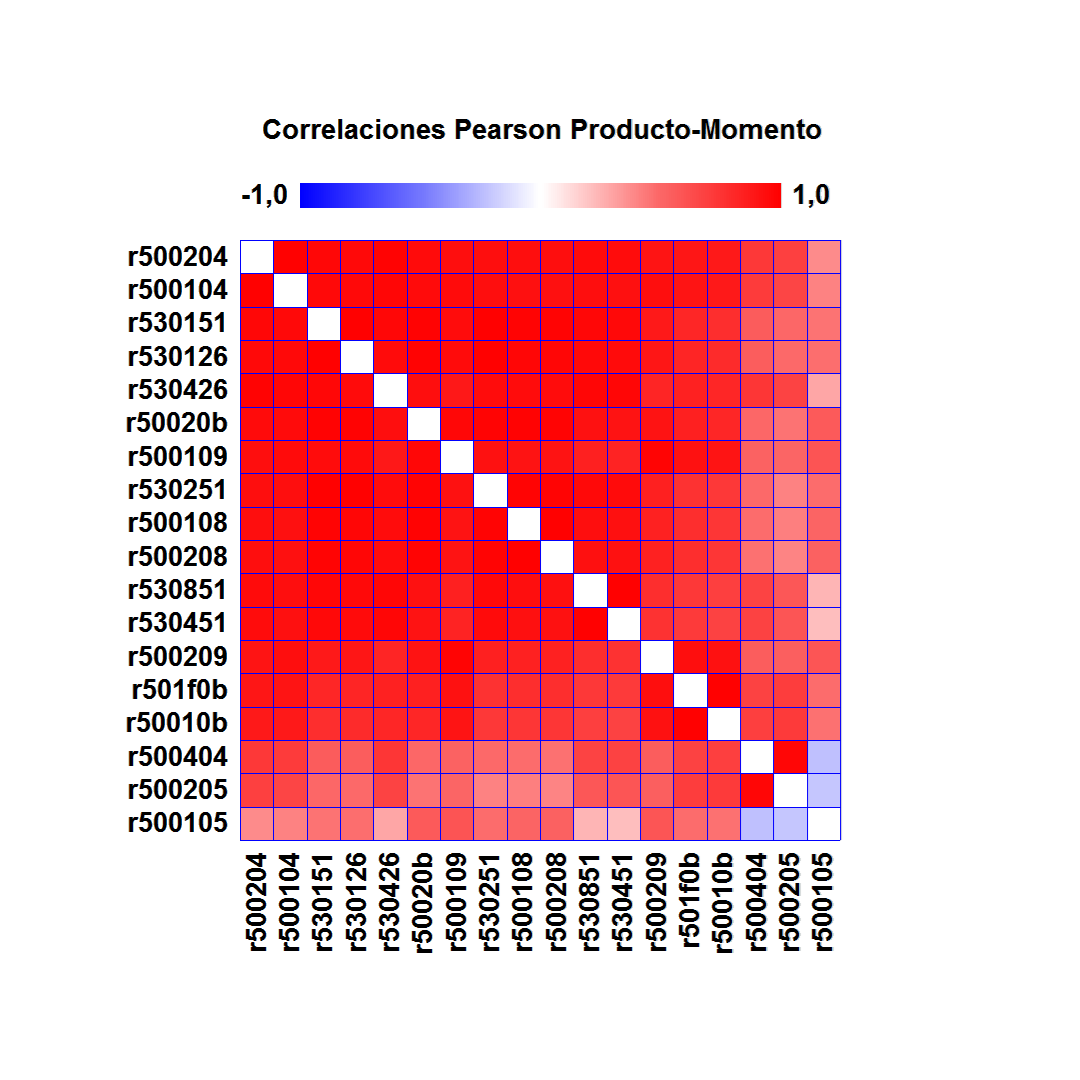
\includegraphics[width=.45\textwidth]{imagenes/corrgram1.png}
		\label{fig:corrgram:b}
	}
	\caption{Resultado de la visualización de la matriz de correlación con el software \emph{statgraphics}. En la figura \ref{fig:corrgram:a} se pueden visualizar los datos en bruto, mientras en \ref{fig:corrgram:b} se presentan los datos agrupados, tras ordenar la matriz de acuerdo al criterio de los vectores propios, logrando un efecto clusterizador.}
	\label{fig:corrmatrix}
	\hspace*{\fill}
\end{figure}

Para ésta tarea, se empleó el software de visualización \emph{statgraphics}\footnote{\url{http://www.statgraphics.com/}} en su edición trial. El software tiene la capacidad de generar una visualización estupénda aprovechando un ordenamiento por medio del primer vector propio de la matriz de correlación misma, de manera de generar un efecto clusterizador sobre los datos, agrupando aquellos con alta correlación.

\subsection{Análisis y Discusión de Resultados}

\subsection{Conclusiones}
A raíz del estudio de canales de comunicación de hardware del sistema se pueden rescatar varios aspectos interesantes:
\begin{itemize}
\item Se identificó un comportamiento creciente en el registro de eventos capturados, trasversal entre todos los eventos postulados en el estudio.
\item La colección de eventos postulada en la tabla \ref{table:codigoseventos} de acuerdo con las componentes de la tabla \ref{table:eventos} registró 2 tendencias principales, una abarcando la gran mayoría de los eventos estudiados y otra, representativa de pocos eventos y de naturaleza exponencial.
\item Al observar en detalle la mayoría de los eventos, se da cuenta de cómo la tendencia de saturación sigue un régimen similar al de los tiempos generales del caso de estudio.
\end{itemize}

\section{Estudio de Distribución de Carga}
La tercera hipótesis de investigación plantea como responsable del mal rendimiento presentado en el caso de estudio al sistema de gestión y administración de tareas en el sistema operativo. En escenarios multicore como el estudiado es normal que el sistema operativo realice como procedimiento de rutina la migración de procesos y la re-alocación de recursos y datos para evitar la saturación de las componentes del mismo. Un caso práctico de ello es cuando un núcleo de procesamiento está sobreexigido y el sistema operativo redistribuye los hilos que están ejecutándose en dicho núcleo entre los otros procesadores disponibles del sistema con el costo que ello significa. Ésta práctica es conocida como \textbf{distribución de carga}, y a pesar de que existen varios mecanísmos de aprovechamiento de dicho esquema como una estratégia de balanceo de carga en arquitecturas como la estudiada \cite{paper:NUMA}, en ciertos escenarios puede degradar el desempeño general del sistema.

Ésta hipótesis plantea que dicho proceso de reasignación de recursos sería perjudicial en escenarios de concurrencia sobre arquitecturas como la estudiada, basandose en que mientras un proceso está en plena ejecución, al incorporar más y más tareas en el mismo nucleo de procesamiento agregando nuevos hilos de ejecución sería el sistema operativo quien comienzaría la reasignación automática de dichos hilos entre los distintos procesadores, cayendo en problemas como perdida de referencias de memoria en niveles de caché primario. En su peor escenario, ésta teoría lleva al ya mencionado problema de \emph{caché bouncing} \cite{paper:cachebouncing} que corresponde al fenómeno de sobre corrección de los datos a nivel de lineas de cache de un procesador, producido por constantes cambios de contexto del \emph{scheduller} que genera migración de procesos. Un problema que ya se mencionó en el estudio de la sección previa.

Una alternativa que se ha estudiado para solventar éste problema es la técnica de \emph{Processor Affinity} que consiste en la asociación de tareas o procesos en CPUs especificas, de manera de controlar la ubicación de memoria y zona real de ejecución del código en la máquina. En otras palabras, se remueve la utilidad del mismo scheduler del sistema operativo para coordinar la mejor operación en la asignación de los hilos de ejecución a las distintas CPU disponible, reemplazándolo por un criterio de diseño humano, construido concientes de la tarea que se desea realizar. Es una técnica muy ambiciosa en el sentido de que bien empleada puede proveer muy buenos resultados en el sistema \cite{paper:cacheaffinity}, sin embargo, es muy facil errar al interpretar el diseño de operación que se desea coordinar, llevando a una mala implementación en la asignación de recursos que termina degradando fuertemente el desempeño del sistema completo.

\begin{defn}[ver AKA AUN NO SE] \textbf{Processor Affinity} Y una bonita defiición de la wea
\end{defn}

En ésta tercer estudio se plantea la utilización de la técnica de \emph{Processor Affinity} en pos de conseguir un mejor rendimiento del caso de estudio presentado, por medio de la reasignación de los hilos de ejecución entre los distintos cores lógicos del sistema. Para evaluar ello, se plantean distintos esquemas de asignación de recursos basados en distintos argumentos arquitecturales del escenario de prueba y se evalúan comparativamente los resultados.


\subsection{Esquemas de Distribución}
Se diseñaron variados esquemas de asignación a fin de evaluar distintos enfoques de aprovechamiento del principio de localidad de memoria. En total se diseñaron 6 esquemas para evaluar combinaciones dinámicas de cores lógicos reconocidos por el sistema operativo en búsqueda de mejores rendimientos. Los esquemas se detallan a continuación:
\begin{description}
\item[Sin Processor Affinity] Asignación dinámica por scheduller del sistema operativo. En éste caso, la elección la hace el sistema de acuerdo a complejos argumentos de prioridad de proceso, carga de cpu, etc. Sirve como punto base de comparación con respecto a los demás esquemas.
\item[DummyAffinity] Asignación directa de hilos a ejecución en el core 0 del sistema. Todos los hilos se delegan al mismo core. Bajo éste esquema se presume que se puede aprovechar mejor la localidad de memoria al disponer en el banco de memoria más próximo al núclo de ejecución todas las referencias necesirias, disminuyendo el efecto de sobrecarga de los protocolos de coherencia y coordinación de cache.
\item[EquitativeAffinity] Asignación secuencial equitativa entre los cores lógicos del sistema, siguiendo la numeración que el sistema operativo dispone de los núcleos mismos. Supone que la distribución completamente justa y equitativa entre cores entrega un mejor rendimiento general.
\item[PairAffinity] Asignación secuencial de hilos a cores de numeración par. Búsca descartar explorar un escenario donde los cores duplicados por efecto de la tecnología \emph{hyperthreading} de Intel pudiera no aprovechar cores reales, y así generar un mejor desempeño final.
\item[ImpairAffinity] Asignación secuencial de hilos a cores de numeración impar. Similar al anterior variando los cores elegidos.
\item[NumaPairAffinity] Asignación de los hilos a cores del segundo conjunto NUMA disponible en el sistema. Sigue la idea de aprovechar toda una unidad lógica de procesamiento según la arquitectura \emph{Quickpath}, persiguiendo mejores tiempos al tener mejor acceso a memoria desde éstos cores.
\item[SimpleCoreAffinity] Asignación de los hilos a los primetos dos cores lógicos del sistema correspondientes al primer core real duplicado por efecto \emph{HyperThreading}.
\end{description}

\subsection{Metodología de Experimentación}

\subsection{Resultados}

Aka muestro los resultados de todos los experimentos
\begin{figure}[!h]
	\centering
	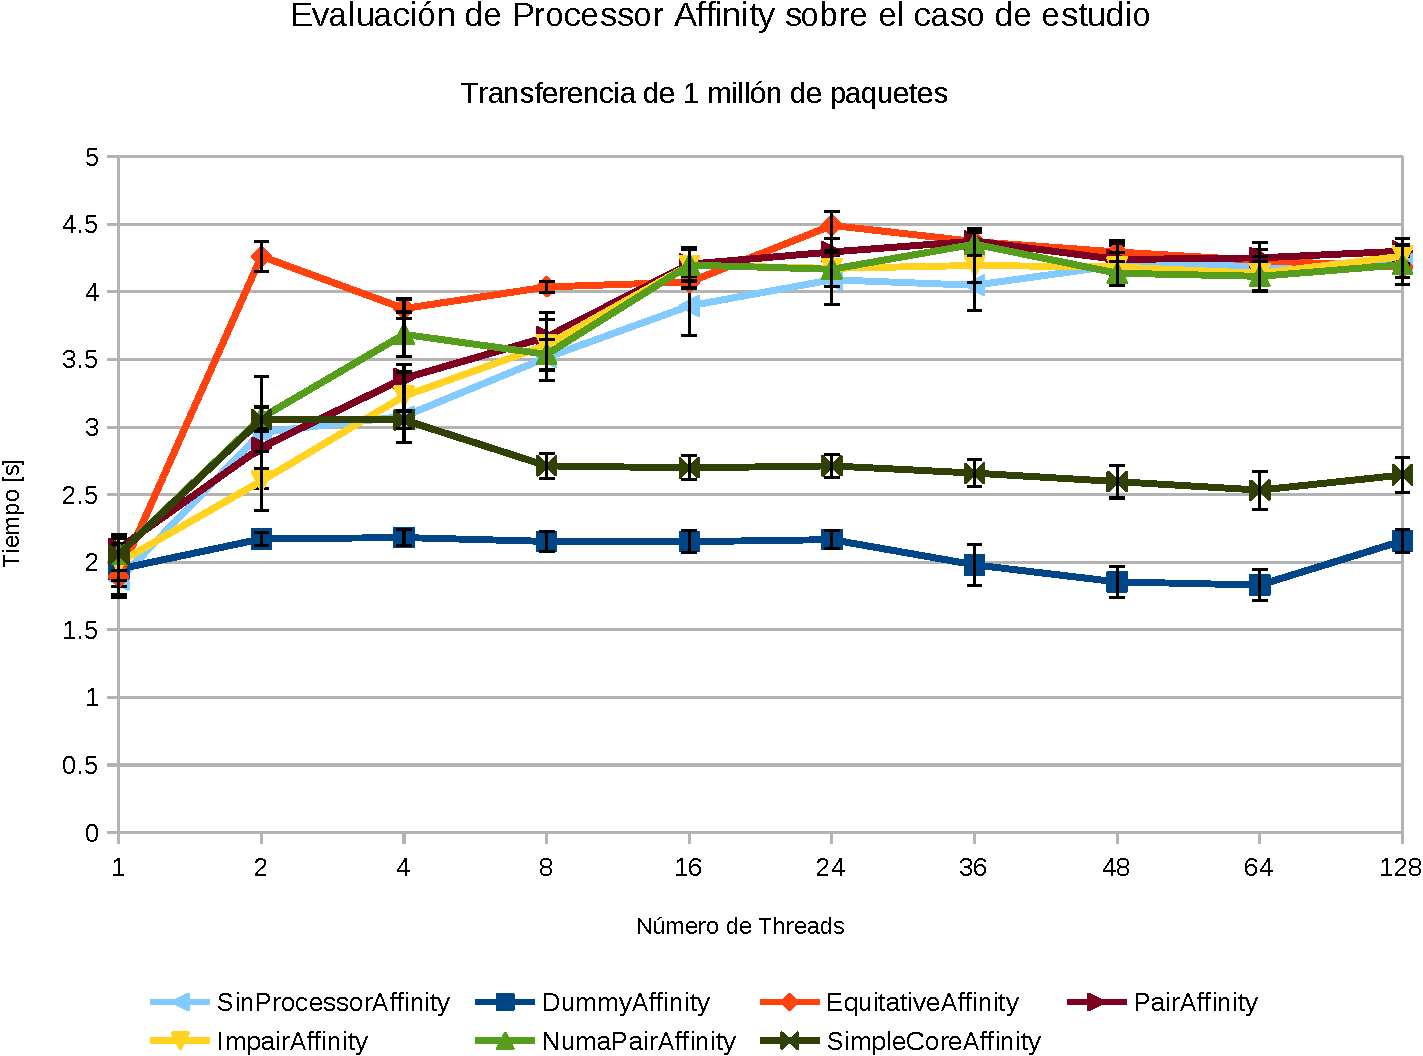
\includegraphics[scale=.6]{resultados/processoraffinity-crop.pdf}
	\caption{Resultados experimentales de los distintos esquemas de afinidad.}
	\label{fig:resAffinity}
\end{figure}

\subsection{Análisis y Discusión de Resultados}
Aka hablar de como es un fiasco la utilización de processor affinity, seguramente porque el scheduller del sistema es mucho más inteligente en la asociación de tareas y threads a los distintos cores. Además la versión con processor affinity es rigida en la localidad del proceso con respecto al procesador lo cual hace que al tener sobrecarga de memoria, los niveles de caché no cooperen con la tarea general, y no brinden beneficio a la prueba final.

\subsection{Conclusiones}
A raíz del estudio de distribución de carga se pueden rescatar varios aspectos interesantes:
\begin{itemize}
\item Las técnicas de processor affinity degradaron aún más el rendimiento de consumo en el caso de estudio, con respecto al caso base de comparación.
\item Los distintos esquemas, a pesar de mostrar variaciones en cada caso, no lograron mejorar con respecto a los tiempos que brindó la administración del mismo sistema operativo.
\item Se vuelve a encontrar en el mismo socket una estructura que se vuelve un punto de contención, calificando al mismo como no apto para soportar accesos concurrentes, ello dado su diseño y mecanísmos de protección implementados (aka. el spinlock interno).
\end{itemize}


\chapter{Estudio de Operación Primitivas de Sincronización del Sistema}

La primera hipótesis a estudiar plantea que el bajo rendimiento de la operación de la interfaz de red --Ilustrada en nuestro caso de estudio por medio de los Internet sockets UDP de Linux-- en escenarios de concurrencia, es causado por un mal desempeño de las estructuras que proveen los mecanismos de sincronización para dichos escenarios. Cómo se mencionó en el capítulo anterior, la capacidad multiprocesador de las computadoras modernas provee un mayor poder de cómputo que se postula a ser aprovechado por medio del uso de técnicas de programación paralela, con el cuidado de que en esos contextos de trabajo, los sistemas operativos deben estar preparados para atender situaciones de conflicto en el acceso a los recursos compartidos. Para este propósito, los sistemas operativos proveen de mecanismos de sincronización ya repasados en secciones anteriores que para estructuras de bajo nivel --como los sockets de Internet-- emplean el uso de mecanismos de sincronización de bajo nivel como lo son los spinlocks, que protegen ciertas porciones críticas de la estructura, tal y como se repasó previamente.

En este caso, la primera hipótesis del problema describe que el responsable del mal rendimiento al incorporar concurrencia en las lecturas a un socket es generado por dichas estructuras de protección en el acceso simultáneo, situación que causaría el fenómeno denominado \emph{Contención de Recurso} sobre la estructura compartida, o sobre alguna de las componentes constitutivas de la misma.

\begin{defn}[ver \cite{paper:resourceContention}] \textbf{Contención de Recurso} corresponde a un estado de conflicto en el acceso a un recurso compartido entre distintas componentes de un sistema, producido por una situación de competencia en el acceso al mismo que puede degenerar en escenarios problemáticos como situaciones de bloqueo, conflictos por situaciones de carrera y degradación generalizada de performance, entre otros.
\end{defn}

Para ratificar el planteamiento anterior, se estudió la dinámica de llamadas de sistema presentes al momento de la ejecución experimental del caso de estudio postulado en el capítulo anterior, ello siguiendo otros modelos de recopilación de datos ya evaluados en otros trabajos exitosos en la misma línea \cite{slides:hpPerf} a modo de poder modelar la operación de las primitivas de sincronización a medida que se van agregando hilos de procesamiento en el consumo de una misma estructura socket compartida. De la misma forma, es interesante analizar cómo el socket compartido actúa como un potencial punto de contención, o como alguna de las estructuras internas de limitación en su acceso (como sería el spinlock del socket mismo) tienen responsabilidad en el rendimiento presentado.

\section{Estudio de Llamadas de sistema}

La operación de las primitivas de sincronización que actúan en los procesos de bajo nivel del sistema operativo tienen la característica de estar determinadas por el uso de llamadas a funciones del sistema, ello pues es el mismo sistema operativo (o mejor dicho el núcleo del sistema) aquel que provee una interfaz simple para la invocación de dichas operaciones. Como son llamadas a funciones, es posible cuantificar cuándo y cómo se realizan las mismas pudiendo modelar el proceso completo por medio de este mecanismo.

Como en nuestro caso de estudio interesa inspeccionar el comportamiento de los spinlocks, se debe contemplar la API con que trabaja el sistema para controlar estas estructuras. Existen distintas funciones que proveen variantes en el funcionamiento de los spinlocks para operar en condiciones especiales, y dichos escenarios son presentables a lo largo de la ejecución del caso de prueba del estudio pudiendo impactar el rendimiento final. El objetivo de este estudio concierne un análisis cuantitativo de la cantidad de llamadas a sistema que sean bloqueantes sobre estructuras spinlock y del tiempo que el sistema gasta en dichas condiciones.

En Linux los spinlocks se representan con estructuras \verb=spinlock_t= (incluidas en el archivo \verb= <linux/spinlock.h>=) que básicamente consisten en un campo de \emph{lock} con un valor 1 (si está libre) o 0 (si está ocupado). Existen diversas funciones de atención que aplican distintos tipos de bloqueo \cite{book:spinlocks}:

\begin{description}
\item[void spin\_lock\_init(spinlock\_t *lock);] Inicializa una estructura spinlock y setea su valor inicial de \emph{lock} en 1.
\item[void spin\_lock(spinlock\_t *lock);] Es el bloqueo básico del sistema para tomar el \emph{lock}. Consistente en la espera del \emph{lock} hasta que presente un valor igual 1 para luego setearlo en 0. Dicha espera se realiza con ciclos de \emph{busy-waiting} hasta que se brinde acceso. Es un bloqueo interrumpible por el sistema operativo, tanto por interrupciones de software como de hardware, dando paso a situaciones como que la CPU determine enviar el proceso responsable de la llamada a dormir por falta de recursos, memoria, etc.
\item[void spin\_lock\_irq(spinlock\_t *lock);] Bloqueo que deshabilita interrupciones del procesador local antes de adquirir el spinlock. Se debe cuidar de reactivar las interrupciones luego de liberado el \emph{lock}.
\item[void spin\_lock\_irqsave(spinlock\_t *lock, unsigned long flags);] Similar a la operación de \verb=spin_lock_irq=, pero con la diferencia de que almacena el estado de interrupción previo en el valor \verb=flags=, de manera de que puede restablecerlo fácilmente luego de liberar el \emph{lock}.
\item[void spin\_lock\_bh(spinlock\_t *lock)] Similar a \verb=spin_lock_irq= con la diferencia de que sólo deshabilita las interrupciones de software, manteniendo habilitadas las interrupciones por hardware del sistema.
\item[int spin\_trylock(spinlock\_t *lock);] Intenta obtener el lock en un único intento, evitando entrar en ciclos muertos de espera, y retornar un valor inmediatamente sobre éxito o fracaso en dicha labor. La función retorna un valor distinto de cero si en su primer intento adquiere el spinlock, o 0 sino. Además, se puede usar en todos los contextos de la función \verb=spin_lock= con el cuidado de administrar el contexto de interrupciones producidas durante la ejecución e intento de adquisición del lock.
%\item[bool mutex\_spin\_on\_owner(struct mutex *lock, struct task\_struct *owner)] Bloqueo que opera sobre una estructura de exclusión mutua (\emph{mutex}) que utiliza el enfoque de \emph{Read-Copy-Update} (RCU), en donde los lectores son no bloqueantes. Ésta estructura tiene una sobrecarga menor que las anteriores; Sin embargo, las actualizaciones son más costosas ya que las versiones anteriores de la estructura de datos se deben guardar con el fin de dar cabida a los lectores ya existentes que se sincronizan a través de las barreras del \emph{mutex}. Utilizando el enfoque de la RCU el bloqueo con esta estructura \emph{mutex} asegura que la operación \emph{Test-and-Set} se ejecute en la misma CPU del propietario del \emph{lock}, lo que reduce la cantidad de comunicación de memoria caché (y por consiguiente, el efecto de contención).
\end{description}

Asociadas a las anteriores llamadas de sistema están las variantes \verb=*unlock*= que permiten liberar el elemento de bloqueo (seteando el valor del \emph{lock} de regreso a 1) para recuperar así su disponibilidad para otros procesos.

Para poder rescatar información relacionada a dichas llamadas a sistema existen distintas herramientas de software, las cuales, implementadas por los mismos desarrolladores del kernel de Linux, son capaces de inspeccionar la operación de bajo nivel del sistema para registrar la dinámica de todas las llamadas que sean de interés. En particular, se pueden usar para analizar la dinámica de llamadas bloqueantes antes descritas.

\subsection{Perf}
Perf \cite{slides:perfTools} o también llamado \emph{Perf\_events\footnote{\url{https://perf.wiki.kernel.org/}}} es una herramienta de análisis de performance para entornos Linux. Corresponde a un subsistema del mismo kernel de Linux que provee un completo framework para el estudio de performance del sistema y de programas por medio de la captura de una amplia variedad de fuentes de datos. Perf es capaz de colectar datos por operatividad de software (contadores de software, \emph{tracepoints}, estadísticas de ejecución de funciones, paso a assembler, etc.) y también de colectar información de control de hardware (manejo de PMU, lectura de \emph{performance counters}, etc.) abarcando los principales registros de control que mantiene el sistema en su operación.

\begin{figure}[!h]
	\centering
	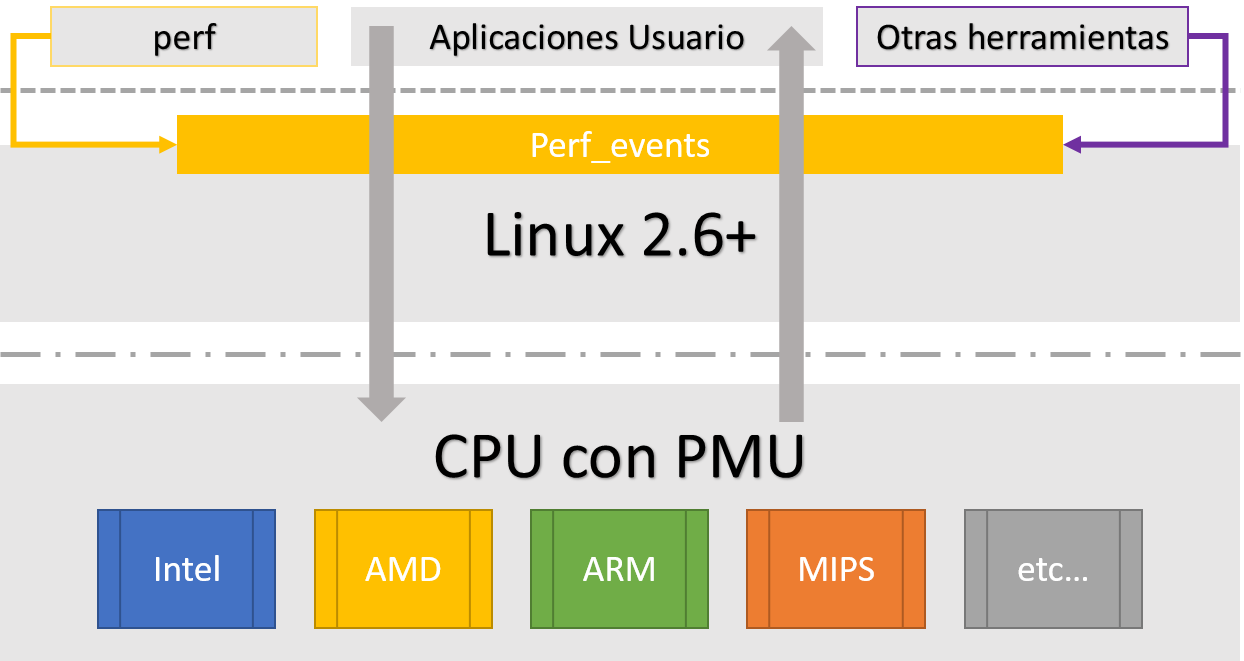
\includegraphics[scale=.45]{imagenes/perfArchitecture.png}
	\caption{Arquitectura de operación del framework provisto por \emph{Perf}.}
	\label{fig:perfFramework}
\end{figure}

Además de su gran capacidad para colectar datos, Perf es una herramienta de sencillo uso. Su funcionamiento se basa en la supervisión de un determinado proceso o tarea de la cual se construye un archivo con la información que se haya seleccionado a colectar \cite{article:perf}. Para ello, se pueden emplear las utilidades \verb=perf-record= y \verb=perf-stat= del framework las que trabajan supervisando un determinado proceso y proveyendo páginas de datos al espacio del kernel de Linux las cuales son escritas con información del sistema de dicho proceso, y son retornadas al espacio de usuario construyendo un informe a modo de output\footnote{La asignación del espacio de páginas a rellenar se hace por medio de la utilidad \verb=mmap= de Linux, que provee direcciones virtuales en un proceso para almacenar información.} (Ver figura \ref{fig:perfRecord}). Esta característica es muy práctica pues se pueden realizar operaciones de análisis más exhaustivos sobre los reportes generados en etapas posteriores a su obtención misma.

El potencial de esta herramienta la perfila como una utilidad indispensable para el estudio en cuestión. En primer lugar por su capacidad de análisis de ejecución de código que permite obtener información cuantificada de las llamadas a sistema y de la dinámica del árbol de llamados\footnote{\emph{Call graph}, correspondiente a un grafo dirigido que representa la relación de llamados entre las subrutinas constitutivas de un proceso principal.} que permite reconocer la naturaleza de las funciones involucradas en el caso de estudio. En segunda instancia Perf es una estupenda herramienta para la recolección de datos de hardware al aprovechar el uso de la \emph{Performance Monitoring Unit (PMU)} del hardware del sistema, una característica que será revisada en detalle en secciones posteriores.

\begin{figure}[!h]
	\centering
	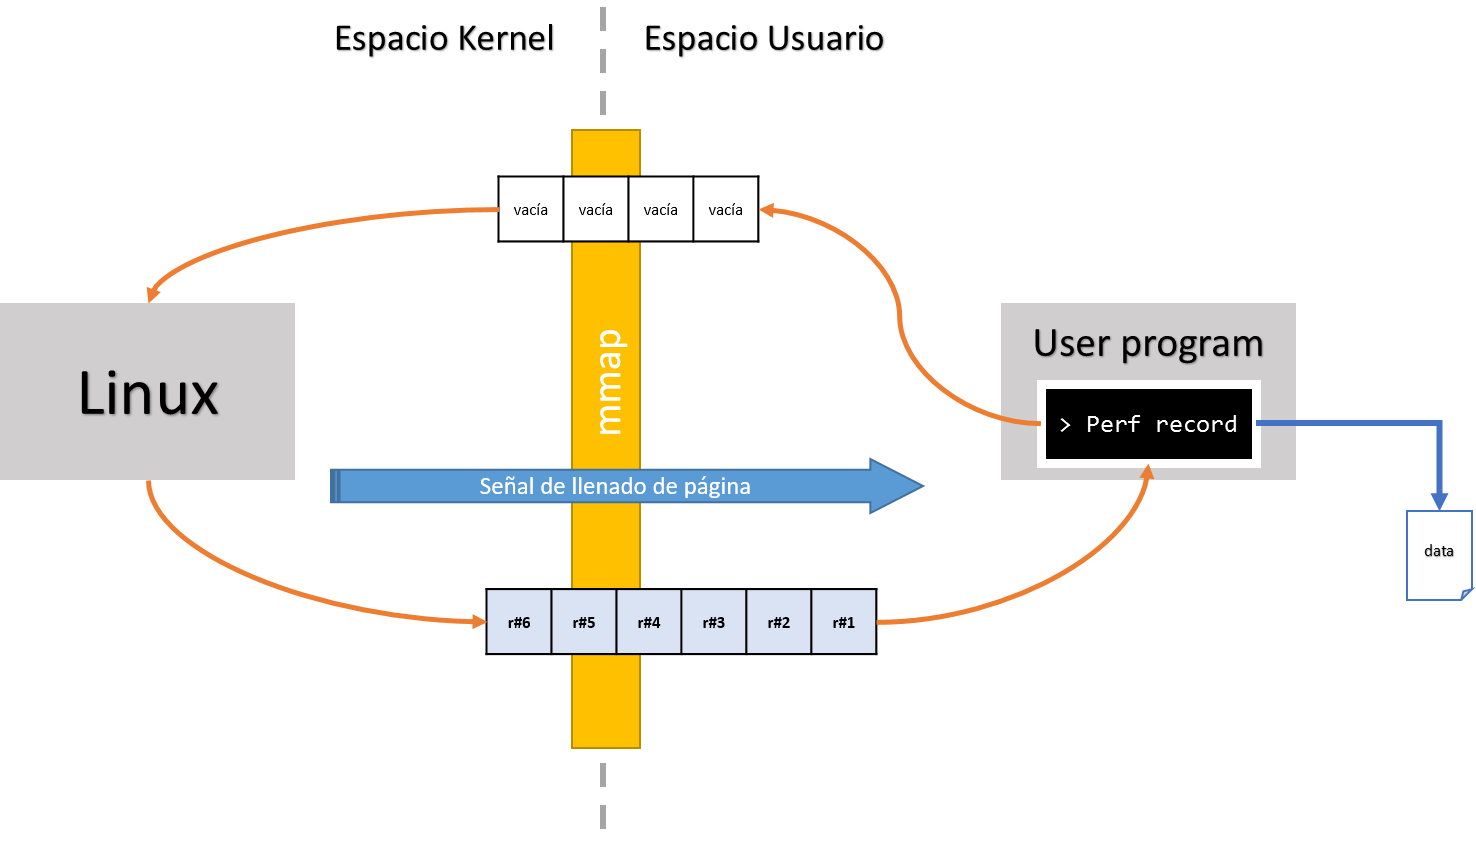
\includegraphics[scale=.52]{imagenes/perfRecord.png}
	\caption{Esquema de captura de datos de un programa usando el comando \emph{perf-record}.}
	\label{fig:perfRecord}
\end{figure}

\subsubsection{FTrace}
FTrace\footnote{\url{http://elinux.org/Ftrace}} es otra poderosa herramienta para análisis de rendimiento de software disponible para sistemas Linux \cite{paper:FTraceSony}. Su funcionamiento opera de naturaleza muy íntima con respecto al kernel mismo pues su recolección de datos se basa en el rastreo de la ejecución de funciones de forma dinámica en el espacio de kernel, caracterizando los tiempos reales de permanencia de cada llamada. Característica que lo hace una estupenda utilidad para el estudio de llamadas al sistema pudiendo recuperar datos como el tiempo de ejecución y cantidad de ocurrencia de las mismas.

Para su uso, FTrace opera como un verdadero framework del sistema sobre el kernel, del cual se pueden usar distintos métodos de rastreo de llamadas. Una de las funciones más poderosas de FTrace es el resultado que se puede obtener por medio de la instrumentación de código, que se refiere a la práctica de incorporar a los programas a analizar \emph{tracepoints} --o puntos de rastreo-- que son declaraciones explicitas de secciones de código a analizar y registrar. A pesar de que esta característica es muy cómoda para programas propios, en el caso del análisis de funciones y llamadas de sistema propias del kernel de Linux, la instrumentación de código es una característica dispensable, siendo sólo necesaria la precisión de qué llamadas a sistema considerar en el análisis pues FTrace es flexible para hacer análisis directamente de funciones del sistema. El uso de esta herramienta es muy flexible y configurable siendo activable a disposición del usuario, una característica muy importante pues al hacer una operación de rastreo de bajo nivel en el sistema, la actividad de FTrace significa una leve degradación en los tiempos netos de actividad de ciertas características del sistema.

En el contexto de la presente investigación, el provecho que se puede sacar de esta herramienta es usar su capacidad para cuantificar tiempo de funciones del kernel de Linux para estudiar la atomicidad de las llamadas bloqueantes del sistema. Así por ejemplo, se pretende determinar el tiempo que se pasa en estados bloqueantes de spinlocks (que terminan siendo pasos de \emph{busy-waiting}) en los cuales sólo se pierde tiempo por efectos de contención de recursos.

\section{Metodología de Experimentación}

Dado que la naturaleza de este estudio se relaciona con el comportamiento de funciones del sistema que administran las primitivas de acceso y sincronización, se realizarán las configuraciones pertinentes para cada herramienta a fin de contemplar dichos puntos de análisis. En el caso de Perf, la recolección de datos se realiza con la herramienta \verb=perf-record=, contemplando un post-procesamiento sobre los archivos de reporte generados a fin de colectar estadísticos asociados a las distintas funciones de manejo de spinlock antes mencionadas\footnote{Experimento \url{https://github.com/sebablasko/Test_MultiThreadStressTransmision} con privilegios de administrador.}.

Por otro lado, para el estudio con FTrace la configuración resulta un poco más compleja. Dado que es una herramienta de traceo dinámico que opera inspeccionando las llamadas de funciones de sistema, la activación de FTrace sobrecarga el funcionamiento del sistema general. Por ello, FTrace se debe activar y desactivar manualmente para analizar sólo los instantes de operación de la prueba de interés. Además, dado el amplio espectro de funciones disponibles para inspeccionar con el framework, se deben emplear las utilidades de filtrado de funciones a inspeccionar que provee el mismo framework, ello en pos de capturar funciones en línea con la dinámica del spinlock del Internet socket.

\vspace{1pc}
\begin{minipage}{\linewidth}
\begin{lstlisting}[style=BashInputStyle, label={code:ftrace}, caption={Configuración de filtros de FTrace sobre funciones a estudiar.}, captionpos=b]
[sebastian@labs-vhost ~]$ echo *spin* > /sys/kernel/debug/tracing/set_ftrace_filter 
[sebastian@labs-vhost ~]$ cat /sys/kernel/debug/tracing/set_ftrace_filter 
mutex_spin_on_owner
spin_msec
_spin_trylock
_spin_lock_irqsave
_spin_lock_irq
_spin_lock
_spin_unlock_irqrestore
_spin_lock_bh
_spin_trylock_bh
_spin_unlock_bh
bit_spin_lock
kvm_vcpu_on_spin
\end{lstlisting}
\end{minipage}

Por otra parte, el encendido y apagado del framework se configuró como parte del script de experimentación en el programa de la prueba\footnote{\url{https://github.com/sebablasko/Test_UDPTrace/}}. En el mismo, se configuró la opción \verb=set_ftrace_pid= para explicitar la inspección de FTrace sólo sobre el programa de la prueba, además del uso de la utilidad \verb=trace_marker= para instrumentar porciones de código de la prueba (como creación de threads, y término de consumo de datos) que permitiese una mayor facilidad al momento de estudiar los logs de ejecución recuperados.


\section{Resultados}
A continuación se ilustran los resultados experimentales obtenidos correspondientes a los datos colectados por Perf y FTrace. A modo de validación estadística, los resultados de las pruebas contemplan el promedio de un rango de 60 repeticiones en cada configuración dada por el caso de estudio.

\begin{figure}[!h]
	\centering
	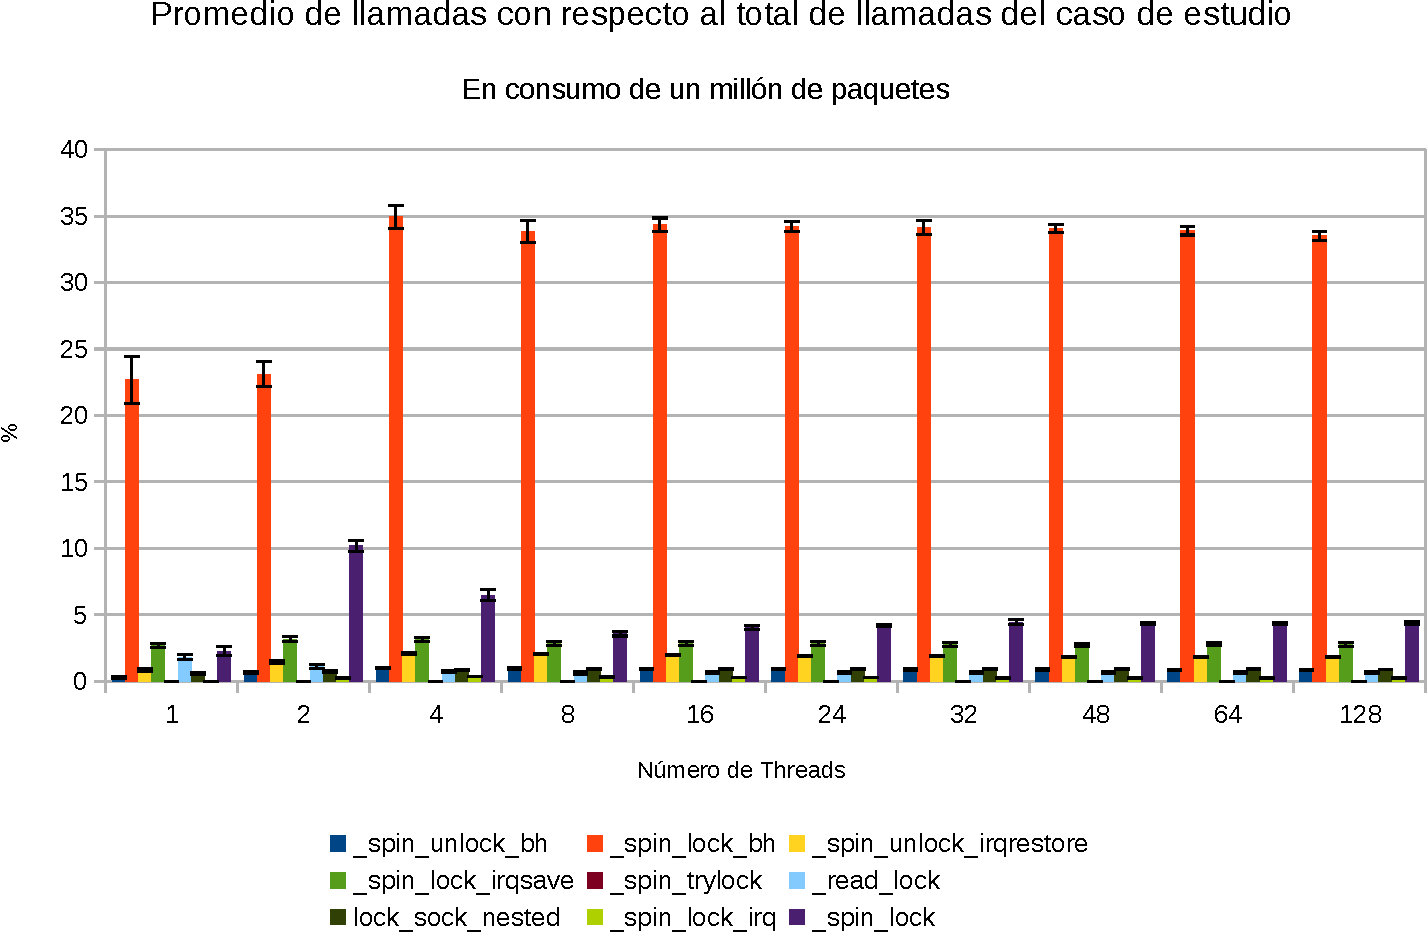
\includegraphics[scale=.6]{resultados/perfdetalle-crop.pdf}
	\caption{Resultados experimentales de los porcentajes de ejecución de las llamadas a sistema recolectadas por \emph{Perf}.}
	\label{fig:resPerf}
\end{figure}

\begin{figure}[!h]
	\centering
	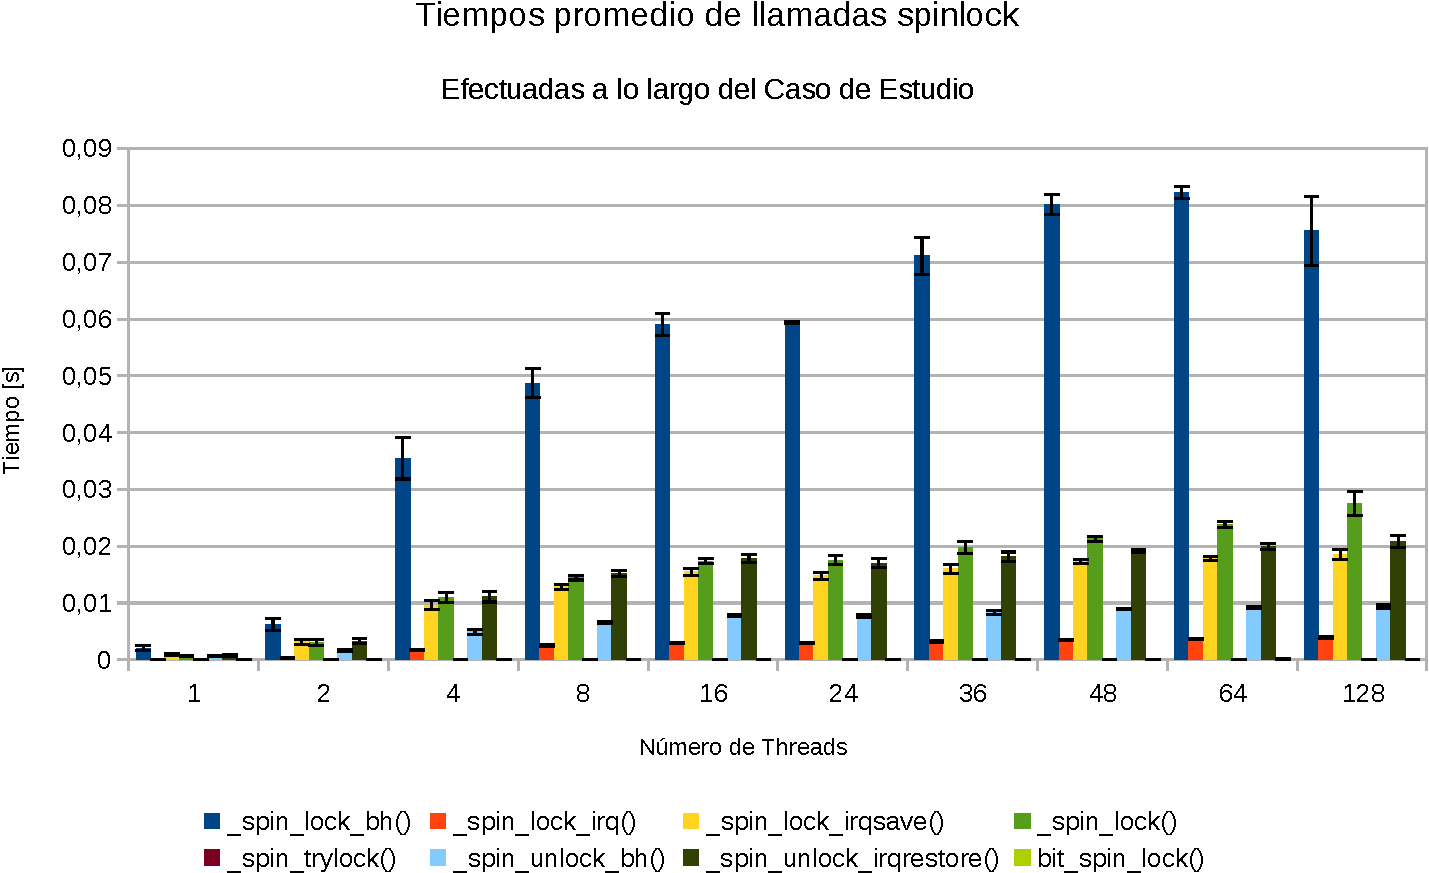
\includegraphics[scale=.6]{resultados/detalleFtrace-crop.pdf}
	\caption{Resultados experimentales de los tiempos de ejecución de las llamadas a sistema recolectadas por \emph{FTrace} para la adquisición y liberación del \emph{lock}.}
	\label{fig:detalleftrace}
\end{figure}


\section{Análisis y Discusión de Resultados}
A primera vista, los resultados corroboran una tendencia creciente de las operaciones (tanto en porcentaje como en tiempo neto de ejecución) de las operaciones de bloqueo sobre spinlock en las pruebas desarrolladas.

En el caso de los resultados de la prueba de Perf disponibles en la imagen \ref{fig:resPerf}, se puede apreciar un comportamiento dominante en el porcentaje de llamado de funciones de una de las funciones por sobre las demás: \textbf{\_spin\_lock\_bh}, llamada que en condiciones de concurrencia puede aumentar su porcentaje de presencia en la ejecución desde un 22\% a casi un 35\%. Otro punto interesante es que, a medida que el escenario se vuelve más competitivo para los threads, los porcentajes rescatados por esta prueba para llamadas de bloqueo aumentan hasta aproximadamente los 4 threads, desde donde se estabiliza, manteniéndose sobre el 40\% sólo en éste apartado.

\begin{figure}[!h]
	\centering
	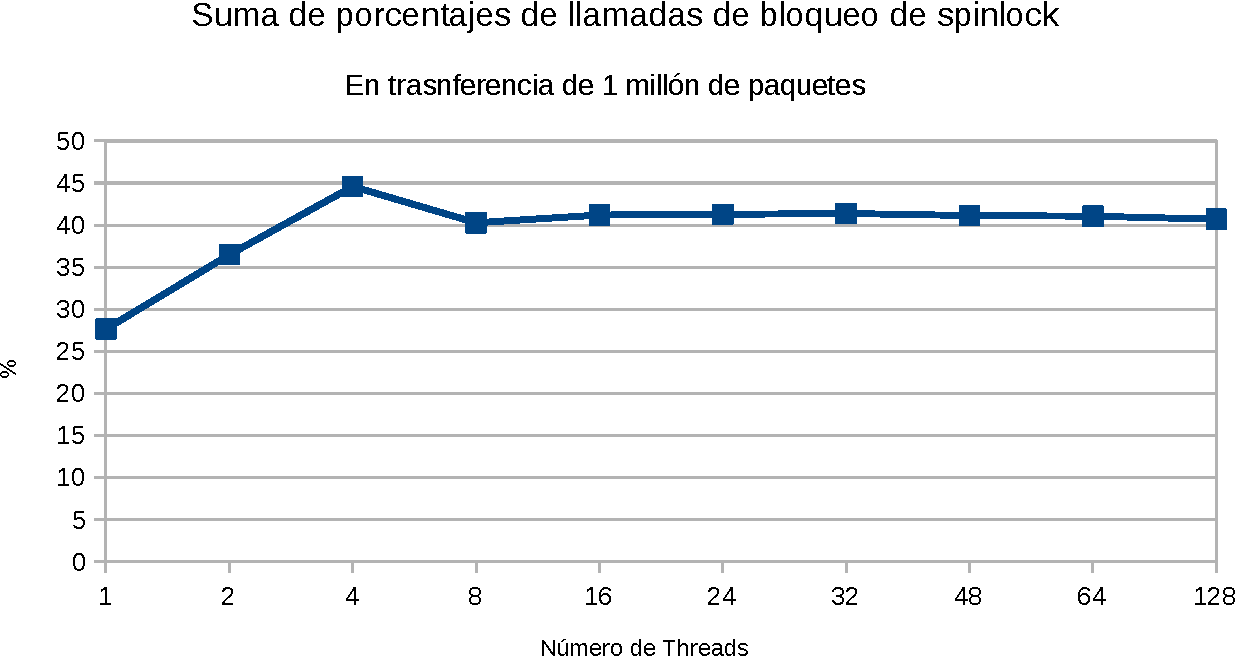
\includegraphics[scale=.6]{resultados/sumaperf-crop.pdf}
	\caption{Gráfico de suma de porcentajes de llamadas de bloqueo del \emph{lock} de spinlock.}
	\label{fig:sumaperf}
\end{figure}

Para reconocer mejor la dinámica de consumo de tiempos en las funciones inspeccionadas en el caso de estudio, se usaron los reportes generados por Perf para construir un nuevo tipo de visualización de llamadas a sistema: Un \emph{Call-Graph-Chart} (Ver imagen \ref{fig:callgraph}), de manera de poder reconocer los bloques de funciones más repetidos en la ejecución del caso de prueba. Para esta visualización se aprovechó el script \emph{gprof2dot}\footnote{\url{https://github.com/jrfonseca/gprof2dot}}. En éste caso, resulta evidente cómo el grafo de llamadas de sistema se complejiza drásticamente al incorporar más threads, de la mano con el aumento en los porcentajes de permanencia en llamadas de sincronización.

\begin{figure}[]
	\centering
	\hspace*{\fill}
	\subfigure[Evaluando 2 Threads]{
		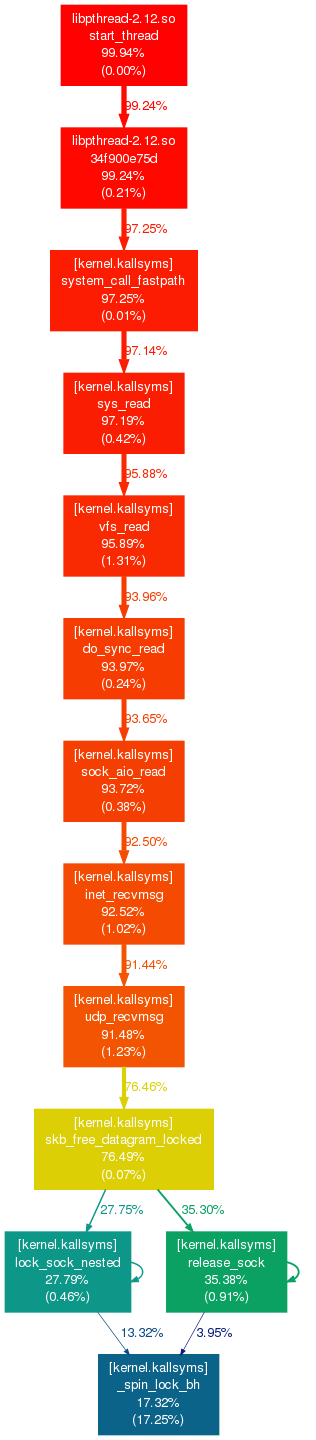
\includegraphics[width=.25\textwidth]{resultados/g2prof_2con.png}
		\label{fig:callgraph2}
	}\hfill
	\subfigure[Evaluando 4 Threads]{
		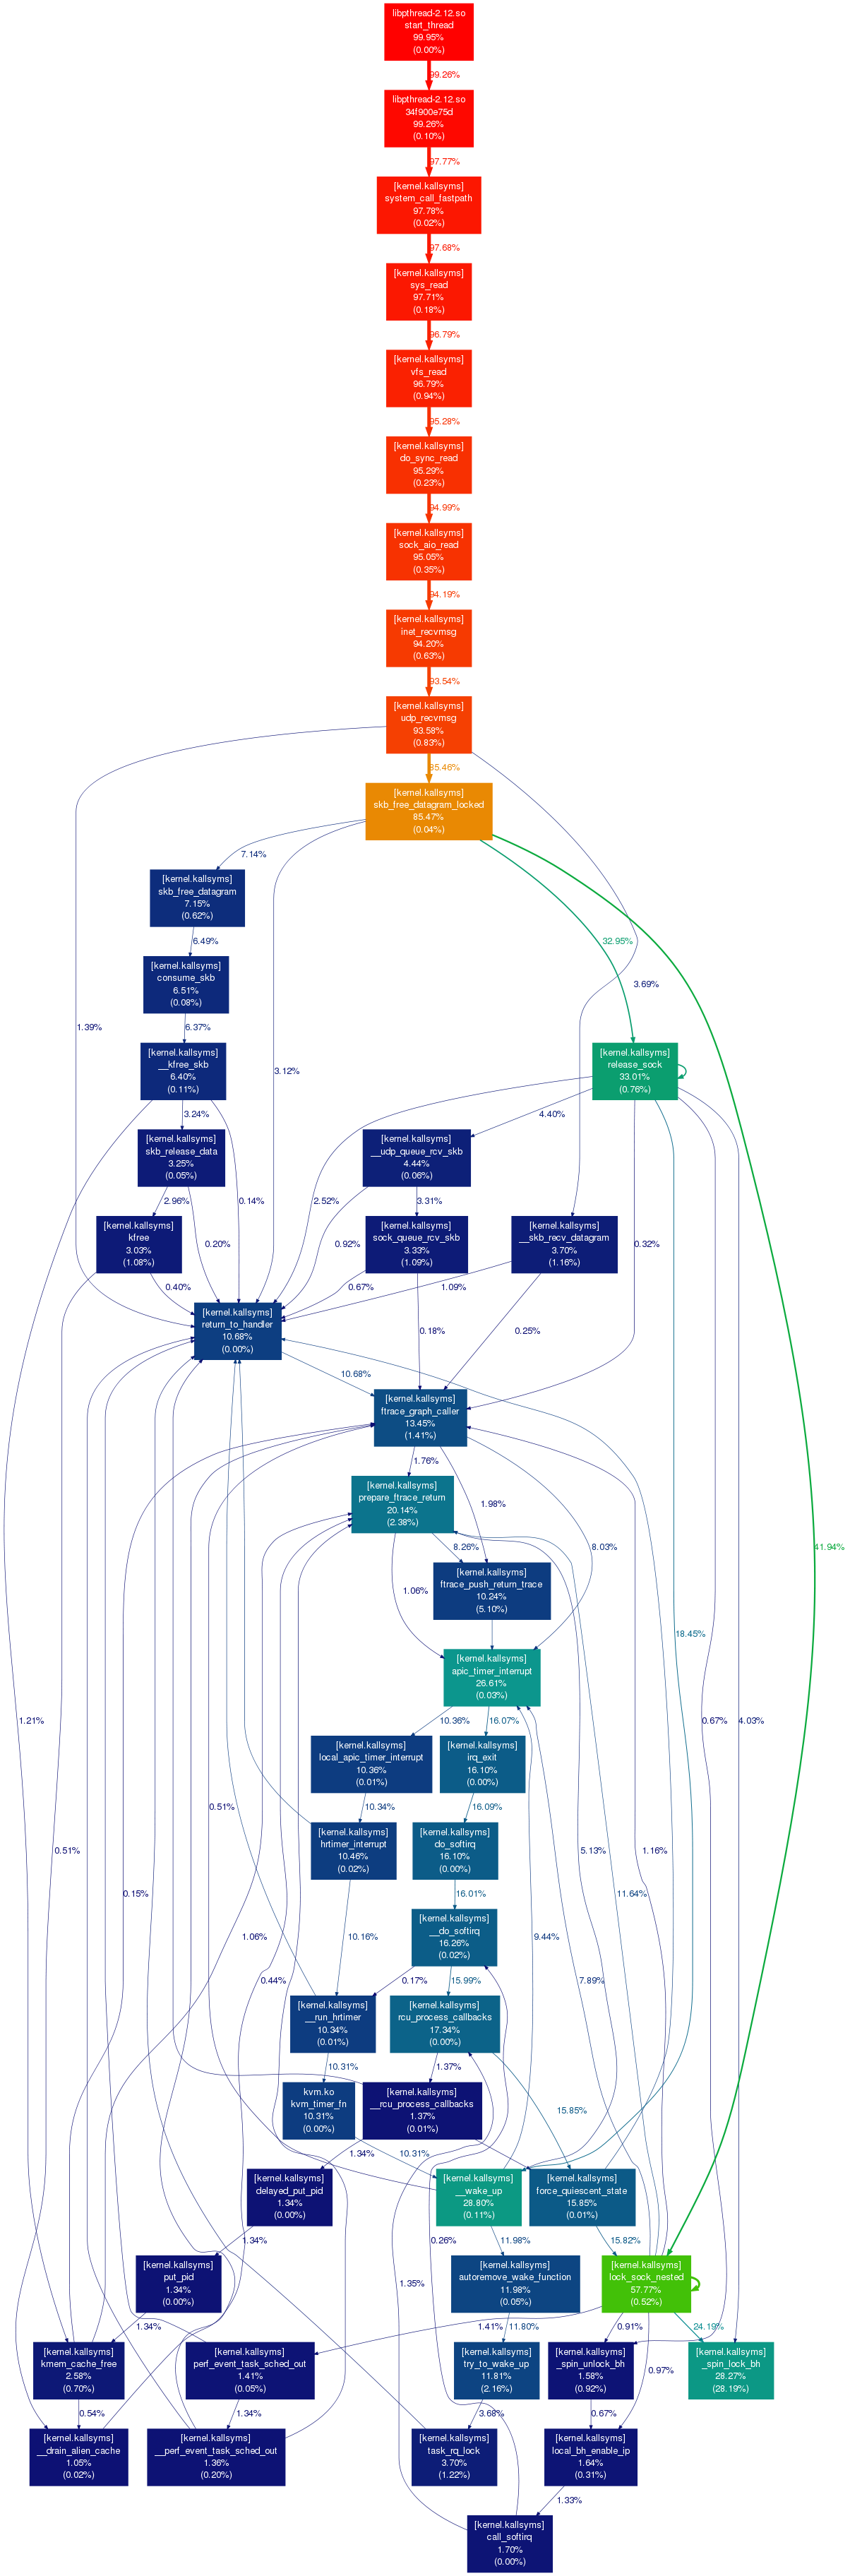
\includegraphics[width=.45\textwidth]{resultados/g2prof_4con.png}
		\label{fig:callgraph4}
	}
	\caption{Visualización de call-graph identificando las llamadas a sistema y sus pesos en el caso de prueba.}
	\label{fig:callgraph}
	\hspace*{\fill}
\end{figure}

Lo anterior postula una primera relación entre el número de threads en el acceso concurrente al socket con respecto al porcentaje y dinámica de llamados a funciones de bloqueo del spinlock. Sin embargo, los porcentajes de llamadas no son del todo relevantes si no se saben los tiempos efectivos que significan en la prueba. Para ello, se repasan los resultados de Ftrace.

Los resultados generales obtenidos con el estudio de FTrace disponibles en la figura \ref{fig:detalleftrace} dan cuenta de un fenómeno aún más interesante. Al igual que con los datos colectados con Perf, se ilustra una estrecha relación entre los tiempos de operación de las funciones relacionadas a spinlock a medida que se van incorporando threads, sin embargo, en éste caso, la tendencia resulta siempre creciente, plasmando cómo a medida que se van usando más threads, el sistema operativo pasa más tiempo en tareas de coordinación en su acceso.

Por otro lado, al realizar una colección de datos con FTrace a modo de recuperar el total de tiempo que se pasa en operaciones de tipo de bloqueo de spinlock se obtiene el resultado ilustrado en la imagen \ref{fig:sumaFtrace}. Una característica interesante de este resultado es que, la tendencia de tiempos producida tiene un ajuste de naturaleza logarítmica, con un índice de determinación superior al 96\%. Este resultado es muy significativo, pues revela que los tiempos reales de acción de las funciones de bloqueo de spinlock siguen una tendencia de la misma naturaleza a los tiempos netos de operación del caso de estudio, estipulando una relación estrecha entre ambos y postulando como principal responsable de los tiempos finales a las funciones de coordinación en el acceso al spinlock.

\begin{figure}[!h]
	\centering
	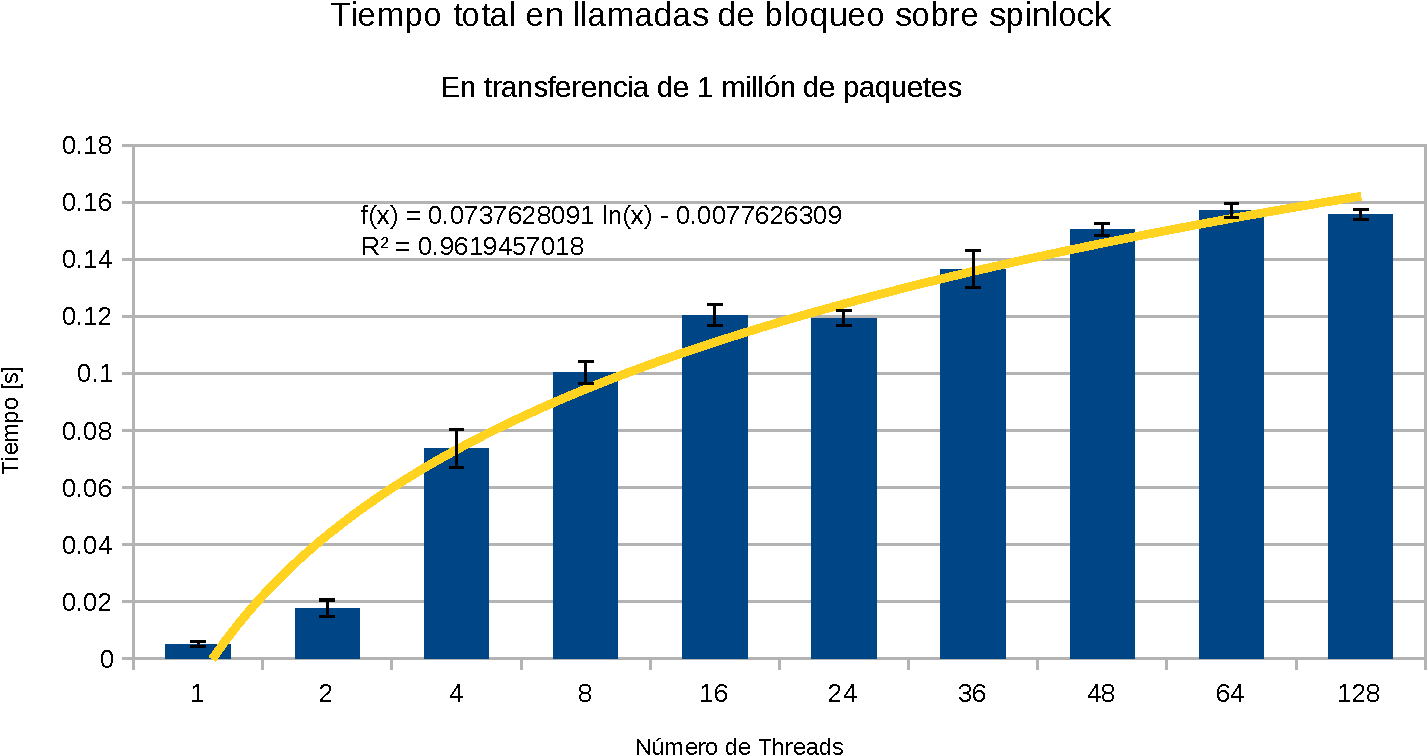
\includegraphics[scale=.6]{resultados/sumaFtrace-crop.pdf}
	\caption{Tiempos totales de bloqueo sobre el \emph{lock} por las distintas llamadas de sistema capturadas por \emph{Ftrace} en el caso de estudio juntos con una curva de aproximación de tendencia.}
	\label{fig:sumaFtrace}
\end{figure}
Más aún, si se repasan las tendencias de cada una de las principales llamadas de bloqueo y de liberación de spinlock (ver figura \ref{fig:Ftracebloquealibera}) se puede ver como las tendencias de naturaleza logarítmica prevalecen al aumentar el número de threads en el consumo de datos. Sin perjuicio de lo anterior, otro dato interesante es que las operaciones de liberación (Fig. \ref{fig:ftracelibera}) son muchísimo más cortas que las de bloqueo (Fig. \ref{fig:ftracebloquea}) revelando el escenario de competencia al que se ve enfrentado el spinlock ante la concurrencia en el acceso.

\begin{figure}[h!]
	\centering
	\hspace*{\fill}
	\subfigure[Funciones de Bloqueo]{
		\includegraphics[width=.47\textwidth]{resultados/bloqueantesftrace-crop.pdf}
		\label{fig:ftracebloquea}
	}\hfill
	\subfigure[Funciones de Liberación]{
		\includegraphics[width=.47\textwidth]{resultados/liberadorasFtrace-crop.pdf}
		\label{fig:ftracelibera}
	}
	\caption{Gráficos con tendencias de tiempos del lock capturados con \emph{Ftrace} a lo largo del caso de estudio.}
	\label{fig:Ftracebloquealibera}
	\hspace*{\fill}
\end{figure}

\subsection{TraceDisplay}
Para poder obtener una interpretación adicional del fenómeno reconocido, se construyó una herramienta de visualización de las llamadas a sistema para funciones de sincronización que permitiese reconocer las porciones de tiempo que tomasen en cada procesador dichas funciones. Para ello, la herramienta denominada \emph{TraceDisplay} recibe un log generado con \emph{FTrace} que incluya las llamadas de sistema ya filtradas, y construye un mapa de tiempo coloreado donde se pueden apreciar las porciones de tiempo que consume cada llamada y desde cual CPU se originan. El resultado se puede apreciar en la imagen \ref{fig:traceDisplay} donde se ilustra el caso de analizar los logs generados por FTrace en un escenario de acceso de 4 threads en el caso de estudio.

Éste subproducto de la investigación principal junto con su documentación de uso está publicado\footnote{Disponible en \url{https://github.com/sebablasko/TraceDisplay}} y disponible para su uso.

\begin{figure}[!h]
	\centering
	\includegraphics[scale=0.34]{imagenes/traceVisualization.png}
	\caption{Visualización de aplicación de llamadas de sistema de sincronización realizadas entre procesadores, generada con la herramienta TraceDisplay.}
	\label{fig:traceDisplay}
\end{figure}

Resultados como el mostrado en la figura \ref{fig:traceDisplay} ilustran como en la práctica, las operaciones de bloqueo se terminan ejecutando secuencialmente, aun cuando son distintos los CPU que los originen. Esto producto de que es una misma estructura la que se está compartiendo la cual no tiene un soporte adecuado para permitir modificaciones concurrentes de orígenes distintos, generando así un sobrecosto producido por dicha serialización en el acceso.


\section{Conclusiones}
A raíz del estudio de operación de primitivas de sincronización del sistema se pueden rescatar varios aspectos interesantes:
\begin{itemize}
\item La tendencia en los costos de tiempo son crecientes a medida que se agregan hilos que consumen el mismo socket. Ello tanto en porcentaje de llamadas de sistema, como también en tiempos netos en dichas llamadas.
\item Se destacan estructuras de tipo spinlock como las más reiteradas en el rastro de llamadas a sistema para la aplicación de mecanismos de protección en el caso de estudio. En particular, la llamada a sistema \textbf{\_spin\_lock\_bh} es la más significativa en la operación de los mecanismos de acceso y toma del \emph{lock} que protege al Internet socket.
\item Se reconoce una significativa diferencia entre los tiempos y porcentajes de llamadas a sistema de tipo bloqueante por sobre los de tipo liberador del \emph{lock}, escenario que da cuenta de la situación de competencia que empeora a medida que se incluyen más threads en la prueba.
\item Se destaca una tendencia de naturaleza logarítmica en el crecimiento de tiempos que toman las llamadas bloqueantes sobre el spinlock del socket, ajustada con un coeficiente de determinación superior al 96\% y que sigue la misma tendencia de los tiempos netos reconocidos en el caso de estudio.
\end{itemize}
A raíz de lo anterior, se reconoce en el spinlock de protección del socket como un punto de cuello de botella al momento de emplear accesos concurrentes a una estructura socket. Ello al actuar como un punto de bloqueo que termina serializando el acceso al consumo de datos y que, lejos de reducir los tiempos paralelizando el acceso, los aumenta, producto de la serialización y de la responsabilidad de coordinar los hilos, propios de este escenario.
\chapter{Estudio de Canales de Comunicación de Hardware}
La segunda hipótesis para explicar la mala performance del caso de estudio presentado se centra en una arista relacionada hardware más que al software mismo. Cómo ya se mencionó, la capacidad multiprocesador de que se dispone en equipos modernos no es un recurso fácil de aprovechar, de hecho, se requiere de una sofisticada operación y diseño tanto de las aplicaciones que solicitan recursos como del sistema operativo que ha de administrarlos, para conseguir las anheladas mejoras de performance. Como se repasó en secciones anteriores, la capacidad de paralelismo viene dada gracias a un conjunto de protocolos y algoritmos de muy bajo nivel que coordinan y mantienen en estado coherente las distintas componentes de datos para los diferentes procesadores disponibles en un esquema \emph{SMP} \cite{paper:MESI, paper:snoop}, sin embargo, por muy sofisticados que dichos mecanismos sean, las nuevas tecnologías de hardware que prometen velocidades de trasferencia y acceso nunca antes imaginadas podrían significar un problema para dichas componentes, sobrepasándolas de cierta forma.

Es precisamente en ésta línea que se establece la segunda hipótesis. En éste caso, se adjudican las responsabilidades por el mal rendimiento presentado en el caso de estudio a un problema de contención de recursos (nuevamente relacionado al spinlock de los Internet sockets), pero ésta vez, asociado a la persistencia y disponibilidad que se da del mismo a través de los mecanismos de coordinación antes mencionados. En las arquitecturas modernas los protocolos \emph{MESI} y de \emph{SNOOP} son cruciales en la operación de ejecuciones paralelas para garantizar integridad en los datos, pero las arquitecturas modernas proponen nuevas distribuciones de los componentes internos de hardware, brindando canales de comunicación de mayor velocidad de transmisión y reasignando los recursos físicos en modos diferentes a los usados para la concepción de los mecanismos de control ya mencionados. Ésta hipótesis plantea la posibilidad de que el defecto de performance del caso de estudio sea generado por un fenómeno de \emph{Caché Bouncing}, producto del abusivo comportamiento de dichos mecanismos de control en las arquitecturas modernas.

\begin{defn}[ver \cite{paper:cachebouncing}] \textbf{Caché Bouncing} corresponde a un fenómeno producido en entornos multiprocesador, cuando distintas CPU realizan modificaciones a una línea de caché especifica que está siendo referenciada por varios procesadores. La modificación de la línea en cuestión se propaga de caché en caché según los protocolos de consistencia del sistema, pero cuando la cardinalidad de referencias de los distintos procesadores sobre la misma línea de caché es muy alta, los mecanismos de propagación de caché pueden operar deficientemente. Éste fenómeno impone una significativa carga en el bus de memoria y los distintos canales de comunicación afectados pudiendo degenerar desde una degradación del proceso responsable hasta una degradación generalizada de la performance del sistema.
\end{defn}

En ésta línea, el fenómeno de \emph{Cache Bouncing} se podría manifestar dada la arquitectura del sistema, la que al contemplar bancos de memoria diversos --algunos compartidos y otros exclusivos para los núcleos de procesamiento-- podría estar manifestándose como resultado de las modificaciones concurrentes de los distintos procesadores sobre la estructura socket compartida, y más precisamente sobre el spinlock de protección del socket. Lo anterior combinado a la operación de los protocolos de consistencia y correctitud para las líneas de caché del sistema postulan evidencia que hace perfectamente posible el diagnóstico de que se esté generando un escenario de sobrecarga de comunicación que termine degradando los tiempos totales de ejecución del caso de estudio.

Para validar la hipótesis anterior es preciso un cabal entendimiento de la arquitectura de hardware objetivo a fin de poder localizar puntos de contención y canales afectados. Junto con lo anterior, se hace crucial una comprensión significativa del funcionamiento de la \emph{Performance Monitoring Unit} que provee el fabricante, así como lograr configurarla y aprovecharla para la recolección de datos finales. En las siguientes secciones se realiza un estudio de la arquitectura descrita en la figura \ref{fig:pc3} del equipo sobre el cual se realizan las pruebas experimentales reales para poder acotar el dominio de estudio. Posteriormente se realiza un análisis experimental de las tendencias presentes en una tarea de acceso concurrente como la descrita en el caso de estudio de ésta investigación con el fin de corroborar o descartar las sospechas ya mencionadas del efecto de contención y \emph{caché bouncing} por eventos de performance de hardware.

\section{Características de Arquitecturas de Hardware Modernas}
Cómo ya se mencionó en secciones anteriores, los fabricantes de partes y piezas de computadoras están constantemente desarrollando importantes avances, de la mano con el desarrollo técnico de piezas que brinda mejores componentes de hardware cada día, y la línea de desarrollo de infraestructura de hardware principal de los computadores no está exenta de dicha evolución. En secciones anteriores se presentó como las arquitecturas han evolucionado desde el primer esquema \emph{SMP} propuesto con la distribución \emph{FSB}, pasando luego por nuevas configuraciones como \emph{DIB} y \emph{DHSI}, entre otras. Sin embargo, el desarrollo ha sido constante y hoy las arquitecturas han degenerado en esquemas bastante más complejos en pos de aprovechar al máximo la capacidad de los procesadores en la línea del paralelismo.

\subsection{Arquitectura Intel QuickPath}
El año 2008, el fabricante de procesadores Intel®\footnote{\url{http://www.intel.com/}} lanzó al mercado una nueva tecnología denominada \emph{Intel QuickPath Architecture} \cite{paper:quickpath} la que postuló un nuevo esquema organizacional de los componentes internos de la placa principal de las computadoras, así como también un nuevo esquema de conectividad entre los componentes de la misma, prometiendo entre otras cosas, un sistema más confiable, eficiente, rápido y escalable, que podría aprovechar mejor la capacidad de los múltiples procesadores de su misma línea. Rápidamente \emph{QuickPath} se posicionó en el mercado para competir con la tecnología \emph{HyperTransport} desarrollada por \emph{AMD}\footnote{Principal competidor de Intel en la industria de la manufactura de microprocesadores.}, abriendo paso definitivamente a una era, dejando atrás el enfoque \emph{FSB}.

\begin{figure}[!h]
	\centering
	\includegraphics[scale=.5]{imagenes/quickpath2.png}
	\caption{Diseño organizacional de los componentes de sistema en una arquitectura estándar \emph{QuickPath} de Intel.}
	\label{fig:quickpath}
\end{figure}

El esquema \emph{QuickPath} postula una reformación arquitectural de los componentes principales de un sistema \ref{fig:quickpath}. En ésta propuesta, las distintas unidades de procesamiento (CPU) están interconectadas por canales de comunicación especiales denominados \emph{Intel QuickPath Interconnect - QPI} que son conexiones punto a punto entre CPU de enorme velocidad de transferencia (llegando hasta 25 GB/s en canales con variantes unidireccional o bidireccional). En línea para aprovechar esta nueva arquitectura, Intel® propone una serie de modificaciones al tradicional protocolo MESI, construyendo el denóminado protocolo \textbf{MESIF} que es una evolución del primero, flexibilizando los protocolos de coherencia de caché al incorporar un nuevo estado para las lineas de caché (\textbf{F} - \emph{Forward}) dotando así de mayor eficiencia y velocidad de acción entre procesadores al ser una comunicación directa.

Por otro lado, en la arquitectura \emph{QuickPath} cada CPU dispone de su propio controlador de memoria y de un banco de memoria de acceso próximo. Dicho diseño se denomina un nodo \textbf{NUMA} de sus siglas en inglés \emph{\textbf{N}on \textbf{U}niform \textbf{M}emory \textbf{A}ccess} [CITA A NUMA] la que permite a las CPU de cada nodo NUMA disponer de un banco de memoria con un acceso garantizado más rápido que al que se tendría acceso en una arquitectura tradicional. El enfoque \emph{NUMA} se aprovecha del principio de localidad de memoria \cite{paper:memorylocality}, por la cual postula que los datos son separables en su acceso por las distintas CPU, logrando así mayor velocidad en el acceso a la memoria, y menor problemas de coherencia de la misma por modificaciones entre CPUs.

El trabajo de Intel® va más allá. Conscientes de la necesidad de herramientas y utilidades para analizar la verdadera performance que provee ésta arquitectura, Intel® provee unidades de monitoreo de performance embebidas en sus procesadores (o \textbf{PMU}, por sus siglas en ingles \emph{\textbf{P}erformance} \textbf{M}onitoring \textbf{U}nit) que son componentes de hardware incorporado a los sistemas que permiten la inspección de operaciones a nivel de comunicación entre componentes del sistema directamente. A éste tipo de análisis se denomina \emph{estudios de Perfomance Counters} dado que para poder realizar una medición, el fabricante de la PMU provee una colección de posibles eventos a colectar, con significaciones puntuales cada uno.

\begin{defn}[ver \cite{KAR00}] \textbf{Performance Counters} son identificadores de máquina que permiten cuantificar determinados eventos a nivel de hardware, como lecturas de caché, corrección de líneas de caché, comunicación de protocolos de coherencia, etc. Usados para analizar el comportamiento de ciertas unidades de hardware y que conforman la base de las herramientas de profiling moderno para el rastreo en el comportamiento de funciones de un sistema.
\end{defn}

La Intel® \emph{QuickPath Architecture} implementa un modelo de 5 capas (Ver fig. \ref{fig:5layersqpi}) para la comunicación de datos entre los núcleos de procesamiento (Similar al espíritu del modelo OSI). De dicho modelo, para la detección de comunicación de aplicaciones son muy significativos los niveles de: \textbf{Protocolo}, al asociar tareas del paso de paquetes, aplicación del protocolo MESIF y de los mecanismos de SNOOP para control y coherencia de líneas de caché, y \textbf{Link}, para el reconocimiento de mecanismos de corrección de errores y recuperación a lo largo de la transmisión de datos entre dispositivos, y para el llamado esquema de \emph{Crédito/Débito} desarrollado por el mismo fabricante que permite trasmisiones de datos confiables entre componentes.

\begin{figure}[!h]
	\centering
	\includegraphics[scale=.5]{imagenes/5layersqpi.png}
	\caption{Diagrama de las 5 capas implementadas en la Intel® \emph{QuickPath Architecture} ilustrando los niveles de control de distintas componentes y protocolos importantes del sistema.}
	\label{fig:5layersqpi}
\end{figure}

El estudio de \emph{performance counters} corresponde a uno de los análisis de más bajo nivel realizables en pos de obtener datos que representen la forma fiel la comunicación entre componentes del sistema. Ello lo hace también un estudio dificultoso de realizar pues amerita un gran conocimiento de la arquitectura puntual sobre el sistema que se desea estudiar, pero de enorme valor para valerse de información sobre la verdadera cuota de comunicación inherente a un caso de estudio.

\section{Especificación y Captura de Eventos}
Para definir el marco conceptual de la prueba, se debe mantener presente el contexto de la hipótesis que fundamenta la misma. En éste caso, la motivación de éste estudio está en línea con entender el comportamiento de un consumo concurrente en una estructura socket, o más precisamente, ver cómo una instancia de una primitiva de sincronización --un spinlock-- se comporta a nivel de actividad de hardware en un escenario multithread. En ese escenario, se busca estudiar cómo se manifestaría la expresión de los protocolos de coherencia de cache bajo circunstancias de ejecución en un escenario mutiprocesador que podrían dar cuenta de que el mal desempeño general del caso de estudio tiene sus origines en los mismos sistemas de coordinación de bajo nivel del sistema.

\subsection{Arquitectura de la máquina para las pruebas}
Siguiendo el caso de prueba evaluado a lo largo de la investigación, se inspeccionará el caso de estudio de saturación de un socket UDP en el equipo servidor multicore para pruebas (Ver fig. \ref{fig:hwspecs}). En éste caso, se cuenta con un equipo placa Dell Inc. 00NH4P A07, provisto de dos CPU Intel Xeon 5600 2.8Ghz, dotado de 6 cores cada uno. Cada CPU dispone de hasta tres niveles de cache de 192 kb, 1536kb y 12288kb respectivamente, que combinados con tres memorias de 4096MB (DDR3 1333MHz) cada uno, conforman 2 nodos NUMA, con un monto total de 24GB de memoria. Una configuración que es precisamente de la familia \emph{Intel QuickPath Architecture} y es enfocada a servidores multicpu \cite{report:intelxeon5600, manual:intelxeon5600}.

\begin{figure}[!h]
	\centering
	\includegraphics[scale=.75]{imagenes/arch24Cores.png}
	\caption{Esquema de arquitectura interna del esquipo servidor multicore sobre el que se realizan las pruebas de \emph{performance counters}.}
	\label{fig:hwspecs}
\end{figure}

Para inspeccionar el sistema donde se evalúan las pruebas en detalle en busca de componentes de monitoreo disponibles se utilizó la utilidad \emph{libpfm4}\footnote{\url{http://www.bnikolic.co.uk/blog/hpc-prof-events.html}} que corresponde a una herramienta confeccionada para recuperar información sobre los códigos de inspección de eventos de performance counters de un sistema y de las PMU disponibles en el mismo. De ello, se da cuenta de que para el modelo de procesador presente se dispone de 5 unidades de PMU disponibles, separables en 3 grupos (Ver código \ref{code:pmuavailable}):
\begin{description}
\item[PMU Genéricas] Incluyen a \verb=perf= y  \verb=perf_raw=. Disponen de las especificaciones estándar de \emph{performance counters} de la línea del software \emph{Perf}, lo cual las hace poco exactas en los valores descritos por cada evento y no necesariamente fieles a su especificación pues dependen en gran parte de que el fabricante sea riguroso en su implementación.
\item[PMU x86] PMU generacional de Intel para la línea x86 de Intel que incluye a \verb=ix86arch=. Dispone de eventos comunes a dicha línea de procesadores por lo que no da soporte específico para la arquitectura \emph{QuickPath} ni del funcionamiento multiprocesador.
\item[PMU westmere] PMU específicas de la línea Westmere [AKA UNA CITA] que soporta la base del desarrollo de la \emph{Intel QuickPath Architecture}, incluyendo a \verb=wsm_dp= y \verb=wsm_unc=. Es el nivel más exacto de PMU que provee el fabricante con los eventos más especificos y documentados del sistema, por lo que es la PMU más importante a la hora de colectar eventos.
\end{description}

\vspace{1pc}
\begin{lstlisting}[style=BashInputStyle, label={code:pmuavailable}, caption={Listado de \emph{PMUs} disponibles en el sistema, recuperado con la herramienta \emph{libpfm4}.}, captionpos=b]
	Detected PMU models:
[18, ix86arch, "Intel X86 architectural PMU", 6 events, 1 max encoding, 7 counters, core PMU]
[51, perf, "perf_events generic PMU", 104 events, 1 max encoding, 0 counters, OS generic PMU]
[53, wsm_dp, "Intel Westmere DP", 91 events, 2 max encoding, 7 counters, core PMU]
[54, wsm_unc, "Intel Westmere uncore", 52 events, 1 max encoding, 9 counters, uncore PMU]
[114, perf_raw, "perf_events raw PMU", 1 events, 1 max encoding, 0 counters, OS generic PMU]
\end{lstlisting}

\subsection{Metodología de captura de eventos}
Para la especificación de la captura de eventos resulta imprescindible prestar especial atención a la arquitectura interna que soporta la comunicación interprocesador del sistema. En la figura \ref{fig:hwcomm} se da cuenta de los canales de comunicación que dispone el sistema estudiado, haciendo un acercamiento a cada unidad lógica de procesamiento, núcleo de cada nodo NUMA.

\begin{figure}[!h]
	\centering
	\includegraphics[scale=.8]{imagenes/QuickPathChannels.png}
	\caption{Esquema de arquitectura interna del equipo servidor multicore estudiado, ilustrando las vías de comunicación del procesador que da cuenta de los principales puntos de alta comunicación en el escenario de \textit{cache bouncing} por contención de valores.}
	\label{fig:hwcomm}
\end{figure}

La figura \ref{fig:hwcomm} da cuenta de los distintos puntos en que se pueden suceder escenarios de congestión dados ya sea por un alto nivel de uso de los protocolos de coordinación de memoria o por un alto tráfico de comunicación entre CPUs. Dichos canales de comunicación podemos resumirlos en las siguientes funciones dedicadas de la arquitectura estudiada, que a su vez están asociadas a ciertos \emph{performance counters} del sistema:

\begin{itemize}
\item Uso de los canales \emph{Intel QuickPath QPI}
\item Acciones del protocolo \emph{SNOOP}
\item Pasos de datos entre distintos caché y memoria
\item Transiciones del protocolo \emph{MESI(F)}
\end{itemize}

Con ello en mente, se consultó el manual oficial del fabricante \cite{manual:bigbigevents} en búsqueda de documentación acerca de eventos disponible en el sistema que se relacionaran a las operaciones antes descritas. De dicha documentación, combinado con la utilidad \emph{libpfm4} para la recolección de eventos disponibles se colectaron un total de 143 eventos cada uno con hasta 6 variantes de configuración, dando en total casi 500 posibles eventos a estudiar. En este escenario es preciso acotar los eventos a considerar, de acuerdo a los 4 criterios antes descritos.


%[[[Hablar un poco de dicha busqueda y del manual]]]]

Finalmente, siguiendo los 4 criterios de puntos problemáticos a estudiar se construyó una selección de eventos a considerar resumida en la tabla \ref{table:eventos}. Los eventos están divididos en dos grupos: \textbf{QPI/GQ/Cache} para eventos relacionados con movimiento o traslación de datos entre distintas unidades de hardware, y \textbf{LinkLayer} para eventos referidos a protocolos de consistencia y sincronización que son pertinentes a la capa de corrección en el esquema de capas del \emph{Quickpath}.

\begin{table}[h!]
\centering
\begin{tabular}{l|l}
\multicolumn{1}{c|}{{\bf QPI/GQ/CACHE}} & \multicolumn{1}{c}{{\bf LinkLayer}} \\ \hline
{ UNC\_GQ\_DATA\_FROM} & SNOOPQ\_REQUESTS \\
{ UNC\_GQ\_DATA\_TO} & SNOOPQ\_REQUESTS\_OUTSTANDING \\
{ UNC\_QHL\_REQUESTS} & SNOOP\_RESPONSE \\
{ L1D} & UNC\_QPI\_RX\_NO\_PPT\_CREDIT \\
{ L2\_DATA\_RQSTS} & UNC\_QPI\_TX\_STALLED\_MULTI\_FLIT \\
{ UNC\_LLC\_HITS} & UNC\_QPI\_TX\_STALLED\_SINGLE\_FLIT \\
{ UNC\_LLC\_MISS} & UNC\_SNP\_RESP\_TO\_LOCAL\_HOME \\
{ UNC\_LLC\_LINES\_IN} & UNC\_SNP\_RESP\_TO\_REMOTE\_HOME \\
{ UNC\_LLC\_LINES\_OUT} & UNC\_IMC\_RETRY
\end{tabular}
\caption{Total de eventos inspeccionados y estudiados en el caso de estudio de consumo concurrente sobre sockets UDP.}
\label{table:eventos}
\end{table}

Con los eventos a colectar más claros, el siguiente paso consiste en conseguir los códigos de registro para la adquisición de cada evento. Un código de registro sigue una nomenclatura dada por el fabricante de la PMU y no guarda relación semántica con el valor que reporta, pero es la única referencia para indicar al software de recolección de datos el evento de interés a estudiar. Para ello, se confeccionó una herramienta\footnote{\url{https://github.com/sebablasko/libpfm4PerformanceEventParser}} para la obtención de los códigos de registros de cada evento de interés la cual trabajando en conjunto con \emph{libpfm4} es capaz de parsear datos del sistema para generar una colección de códigos de registro asociados a eventos de hardware en formato \verb=JSON=, según los cuales se tiene una correcta representación del nivel de saturación y uso de los componentes. Con el \verb=JSON= generado, se pueden hacer mediciones de forma sencilla usando la herramienta \verb=stat= de \emph{Perf} para generar un reporte de la cantidad de veces que se registre actividad en el evento estudiado, especificado en la misma herramienta.

\vspace{1pc}
\begin{lstlisting}[style=BashInputStyle, breaklines=true, captionpos=b, caption={Ejemplo de uso de Perf para colectar datos de una colección de eventos. En éste caso se configura para colectar datos de 2 eventos y dejar el reporte en un archivo de salida.}]
	# perf stat -e r53003c,r5300c0 -o resultado.txt -- ./programa
\end{lstlisting}

Finalmente, de los output de Perf se pueden estudiar los resultados finales de la comunicación efectiva generada a lo largo de la prueba.

\section{Metodología de Experimentación}
Para poder comprender mejor las tendencias de comportamiento de los distintos eventos en cada instancia de prueba con una determinada configuración de threads, se confeccionó un experimento donde se evaluaron 3 escenarios de consumo para comparar sus resultados\footnote{\url{https://github.com/sebablasko/Test_PerformanceCounters}}:

\begin{enumerate}
\item Lectura concurrente desde un dispositivo virtual como \verb=dev_null=. Para ilustrar el comportamiento en el caso de menor sobrecarga en lectura concurrente al ser un dispositivo libre de barreras de bloqueo.
\item Lectura exclusiva desde un socket UDP. En éste caso se consume la cuota definida en el caso de estudio por sockets con acceso exclusivo, distribuyendo la carga entre ellos con sólo 1 thread por socket. 
\item Lectura concurrente desde un socket UDP. Precisamente el caso de estudio evaluado a lo largo de toda la investigación.
\end{enumerate}

Así se puede tener un punto de comparación del fenómeno que se manifiesta en escenarios de lectura concurrente sobre un socket, y que no se manifiesta en otros escenarios.

Para la recolección de datos se empleó nuevamente el software \emph{Perf} para la administración y control de la PMU del sistema. Al igual que en el caso de estudio original se evalúan configuraciones de 1, 2, 4, 8, 16, 24, 36, 48, 64 y 128 threads contemplando un total de 60 repeticiones del proceso de captura para cada configuración de prueba. En la recolección de datos se define $T_i$ a la tupla que agrupa los resultados de cada una de las 60 repeticiones para una configuración de la prueba empleando $i$ hilos.

\begin{equation}
\label{eq:tupla1}
T_i = \left\{ T_{i,1},T_{i,2},T_{i,3}, \dots ,T_{i,59}, T_{i,60}\right\} 
\end{equation}

Con las muestras totales para cada configuración, se pueden determinar representantes estadísticos que nos permitan ilustrar el valor de cada configuración. Para éste propósito se emplea el calculo del promedio simple entre las muestras.

\begin{equation}
\label{eq:promedio}
\overline{T_{i}} = \frac{T_{i,1}+T_{i,2}+T_{i,3}+ \dots +T_{i,59}+ T_{i,60}}{60}
\end{equation}

Finalmente, se construye con para cada evento estudiado un set de registros que guardan el valor promedio de cada evaluación en una determinada configuración de hilos de ejecución.

\begin{equation}
\label{eq:tupla2}
Evento_j = \left(\overline{T_{1}}, \overline{T_{2}}, \overline{T_{4}}, \overline{T_{6}}, \overline{T_{8}}, \overline{T_{16}}, \overline{T_{24}}, \overline{T_{36}}, \overline{T_{48}}, \overline{T_{60}}\right)
\end{equation}

De ésta manera, se pueden hacer análisis más simples sobre las variables aleatorias $Evento_j$ que permita una simple comparación entre cada una de los 3 escenarios de evaluación estipulados.

\section{Resultados}
Dada la enorme cantidad de resultados obtenidos en el proceso de inspección de los \emph{performance counters}, se presentan sólo aquellos resultados con comportamiento interesante registrado en el caso de prueba.

Los resultados se han agrupado en 8 categorías para facilitar la asociación de comportamientos y de elementos analizados: Comportamiento de caché de datos de nivel 1, caché de nivel 2, último nivel de caché y banco de memoria, fallo en predicción de procesamiento, solicitudes fuera del core, comunicación por canales de la arquitectura \emph{Quickpath} y finalmente actividad de coordinación por protocolos \emph{SNOOP} y \emph{MESIF}.

\begin{figure}[ph!]
\centering
\subfigure[]{
	\includegraphics[width=.47\textwidth]{resultados/pcounters/r530151.png}
	\label{fig:pcounterL1a}
}
\subfigure[]{
	\includegraphics[width=.47\textwidth]{resultados/pcounters/r530251.png}
	\label{fig:pcounterL1b}
}
\subfigure[]{
	\includegraphics[width=.47\textwidth]{resultados/pcounters/r530451.png}
	\label{fig:pcounterL1c}
}
\subfigure[]{
	\includegraphics[width=.47\textwidth]{resultados/pcounters/r530851.png}
	\label{fig:pcounterL1d}
}
\caption{Resultados asociados al comportamiento del caché de datos de primer nivel.}
\label{fig:pcounterL1}
\end{figure}

\begin{figure}[ph!]
\centering
\subfigure[]{
	\includegraphics[width=.47\textwidth]{resultados/pcounters/r530f28.png}
	\label{fig:pcounterMESIFa}
}
\subfigure[]{
	\includegraphics[width=.47\textwidth]{resultados/pcounters/r530128.png}
	\label{fig:pcounterMESIFb}
}
\caption{Resultados asociados al comportamiento del protocolo MESIF.}
\label{fig:pcounterMESIF}
\end{figure}

\begin{figure}[ph!]
\centering
\subfigure[]{
	\includegraphics[width=.47\textwidth]{resultados/pcounters/r537f89.png}
	\label{fig:pcounterMissBranchPredictiona}
}
\subfigure[]{
	\includegraphics[width=.47\textwidth]{resultados/pcounters/r5301c5.png}
	\label{fig:pcounterMissBranchPredictionb}
}
\caption{Resultados asociados al fenómeno de fallo en predicción de ejecución del procesador.}
\label{fig:pcounterMissBranchPrediction}
\end{figure}


\begin{figure}[ph!]
\centering
\subfigure[]{
	\includegraphics[width=.47\textwidth]{resultados/pcounters/r5301b0.png}
	\label{fig:pcounterOFFCorea}
}
\subfigure[]{
	\includegraphics[width=.47\textwidth]{resultados/pcounters/r5380b0.png}
	\label{fig:pcounterOFFCoreb}
}
\subfigure[]{
	\includegraphics[width=.47\textwidth]{resultados/pcounters/r530160.png}
	\label{fig:pcounterOFFCorec}
}
\caption{Resultados asociados al comportamiento de fallo en solicitud de datos de un core.}
\label{fig:pcounterOFFCore}
\end{figure}

\begin{figure}[ph!]
\centering
\subfigure[]{
	\includegraphics[width=.47\textwidth]{resultados/pcounters/r53aa24.png}
	\label{fig:pcounterL2a}
}
\subfigure[]{
	\includegraphics[width=.47\textwidth]{resultados/pcounters/r53e027.png}
	\label{fig:pcounterL2b}
}
\subfigure[]{
	\includegraphics[width=.47\textwidth]{resultados/pcounters/r530f26.png}
	\label{fig:pcounterL2c}
}
\subfigure[]{
	\includegraphics[width=.47\textwidth]{resultados/pcounters/r5302f1.png}
	\label{fig:pcounterL2d}
}
\subfigure[]{
	\includegraphics[width=.47\textwidth]{resultados/pcounters/r530127.png}
	\label{fig:pcounterL2e}
}
\caption{Resultados asociados al comportamiento del caché de segundo nivel.}
\label{fig:pcounterL2}
\end{figure}


\begin{figure}[ph!]
\centering
\subfigure[]{
	\includegraphics[width=.47\textwidth]{resultados/pcounters/r50010b.png}
	\label{fig:pcounterLLCa}
}
\subfigure[]{
	\includegraphics[width=.47\textwidth]{resultados/pcounters/r50012e.png}
	\label{fig:pcounterLLCb}
}
\subfigure[]{
	\includegraphics[width=.47\textwidth]{resultados/pcounters/r50022e.png}
	\label{fig:pcounterLLCc}
}
\subfigure[]{
	\includegraphics[width=.47\textwidth]{resultados/pcounters/r500109.png}
	\label{fig:pcounterLLCd}
}
\subfigure[]{
	\includegraphics[width=.47\textwidth]{resultados/pcounters/r500308.png}
	\label{fig:pcounterLLCe}
}
\subfigure[]{
	\includegraphics[width=.47\textwidth]{resultados/pcounters/r530205.png}
	\label{fig:pcounterLLCf}
}
\caption{Resultados asociados al comportamiento del último nivel de caché y memoria principal.}
\label{fig:pcounterLLC}
\end{figure}


\begin{figure}[ph!]
\centering
\subfigure[]{
	\includegraphics[width=.47\textwidth]{resultados/pcounters/r500104.png}
	\label{fig:pcounterQPIa}
}
\subfigure[]{
	\includegraphics[width=.47\textwidth]{resultados/pcounters/r500105.png}
	\label{fig:pcounterQPIb}
}
\subfigure[]{
	\includegraphics[width=.47\textwidth]{resultados/pcounters/r500204.png}
	\label{fig:pcounterQPIc}
}
\subfigure[]{
	\includegraphics[width=.47\textwidth]{resultados/pcounters/r500205.png}
	\label{fig:pcounterQPId}
}
\subfigure[]{
	\includegraphics[width=.47\textwidth]{resultados/pcounters/r500240.png}
	\label{fig:pcounterQPIe}
}
\caption{Resultados asociados al comportamiento los canales y estructuras de comunicación del Intel® \emph{QuickPath}.}
\label{fig:pcounterQPI}
\end{figure}


\begin{figure}[ph!]
\centering
\subfigure[]{
	\includegraphics[width=.47\textwidth]{resultados/pcounters/r5301b4.png}
	\label{fig:pcounterSNOOPa}
}
\subfigure[]{
	\includegraphics[width=.47\textwidth]{resultados/pcounters/r5302b4.png}
	\label{fig:pcounterSNOOPb}
}
\subfigure[]{
	\includegraphics[width=.47\textwidth]{resultados/pcounters/r500106.png}
	\label{fig:pcounterSNOOPc}
}
\subfigure[]{
	\includegraphics[width=.47\textwidth]{resultados/pcounters/r500107.png}
	\label{fig:pcounterSNOOPd}
}
\subfigure[]{
	\includegraphics[width=.47\textwidth]{resultados/pcounters/r500206.png}
	\label{fig:pcounterSNOOPe}
}
\caption{Resultados asociados al comportamiento del mecanísmo de control \emph{SNOOP}.}
\label{fig:pcounterSNOOP}
\end{figure}

\section{Análisis y Discusión de Resultados}

Los diferentes resultados presentados en la sección anterior comparten una serie de características comunes importantes de resaltar: En primer lugar, la experimentación sobre el dispositivo virtual \verb=dev_null= presentó prácticamente un nulo registro a nivel de los eventos contabilizados. Una situación esperable pues como se adelantó al momento de diseñar el experimento, éste dispositivo fue elegido como parte de la prueba por ser un dispositivo virtual libre de protecciones ante concurrencia, de manera que su registro da pistas de la correcta activación de las labores de registro de eventos.

Otro rasgo general interesante es que los comportamientos entre el caso \emph{UDPMultiThread} y \emph{UDPSingleThreadMultiSocket} presentan notables diferencia en prácticamente todos los eventos inspeccionados en el caso de estudio, lo cual, más allá de los distintos valores registrados, corrobora que existe una significativa diferencia entre los dos enfoques de consumo de datos (compartición del socket con múltiples hilos contra consumo exclusivo de socket).

En las secciones siguientes se analizan en detalle cada uno de los grupos de resultados rescatados en ésta prueba.

\subsection{Comportamiento de caché de datos de nivel 1}
Los resultados registrados con respecto al comportamiento del caché de datos de nivel 1 (Ver figura \ref{fig:pcounterL1}) evidencian un claro comportamiento desigual entre los escenarios de consumo concurrente vs. consumo exclusivo. Como se aprecia en la mayoría de los resultados de dicha prueba, las tendencias entre ambos escenarios son similares hasta la aplicación de dos hilos, pero al incorporar más hilos de ejecución rápidamente los registros de eventos contabilizados se disparan en el caso multi-hilo, evidenciando una mayor actividad a nivel de caché de datos de nivel 1.

Otro dato interesante a resaltar es el fenómeno de \emph{caché bouncing} expresado en éste resultado. Cómo se puede apreciar, los resultados de las figuras \ref{fig:pcounterL1b}) y \ref{fig:pcounterL1c}) que expresan la cantidad de líneas de caché en estado modificado (de acuerdo a la nomenclatura \emph{MESI}) aumentan progresivamente a medida que se incrementan los hilos consumiendo datos del socket compartido, apoyando la idea de que el escenario concurrente contribuye a una mayor sobre corrección de líneas de caché, lo que puede contribuir en una degradación de la performance del sistema. Lo anterior es nuevamente avalado por el resultado de la figura \ref{fig:pcounterL1d}), que ilustra la acción de los protocolos de corrección y coordinación para modificar estados de líneas de caché. Vale decir, éste resultado muestra cómo los mecanismos de coordinación del sistema están operando desde componentes ajenas a cada Core para corregir líneas que han sido modificadas en otro procesador, otro indicio de que la modificación concurrente de una estructura compartida termina impactando al sistema completo.

Una última reflexión de éste resultado da cuenta de cómo las tendencias crecientes registradas por los eventos relacionados al caché de datos de nivel 1 se ajustan a la registrada por los tiempos prácticos de ejecución del caso de estudio, dando espacio para entender una correlación entre ambos fenómenos.

\subsection{Comportamiento de protocolo MESIF}
En el caso del protocolo MESIF, los resultados registrados a lo largo del caso de estudio (Ver figura \ref{fig:pcounterMESIF})) dan cuenta de dos situaciones a destacar relacionadas a los eventos detectados por concepto de escrituras de líneas de caché de nivel 1 a nivel 2, fenómeno que indica que un valor presente en ambos niveles de caché sufrió una modificación que hace que se propague hacia los niveles de caché inferiores.
La figura \ref{fig:pcounterMESIFa}) presenta el total de sobre escrituras realizadas desde el caché de datos de nivel 1 al caché de nivel 2. Es fácil notar que las tendencias dominantes nuevamente se atribuyen al escenario multi-hilo, que sobrepasa ampliamente al caso de lectura exclusiva desde un socket. Ésta situación respalda el escenario descrito en el análisis previo sobre el comportamiento de caché de datos de nivel 1, donde las sobre correcciones ocurridas en el sistema producto de la modificación de un recurso compartido termina aumentando excesivamente la comunicación práctica entre componentes. En el caso del resultado de la figura \ref{fig:pcounterMESIFb}) la situación resulta aún más dramática. 

En ese resultado se contabilizan los eventos de sobre escritura desde nivel 1 a nivel 2 sobre líneas que presentan estado \emph{Invalid} de acuerdo al protocolo \emph{MESI}, es decir, corrección de valores que ya fueron descartados por otro componente del sistema. Ésta situación da cuenta de cómo la coordinación a nivel de las líneas de caché se va tornando caótica a medida que se intensifican los escenarios concurrentes en el acceso al socket. Cabe destacar que tal como antes, las tendencias generales de los eventos registrados en el caso concurrente se adecúan mucho con la del tiempo del caso de estudio.

\subsection{Comportamiento de Predicción de ejecución del Procesador}
Una de las características fundamentales de los equipos modernos es la capacidad de anticipación de ciertas operaciones a realizar, ya sea cómputo de ciertos valores así como modificaciones o accesos a porciones de memoria. Para ello, durante la ejecución de un programa en que pueden continuar distintas secuencias de pasos, el sistema pre calcula el valor de algunos flujos a seguir de manera de anticiparse a dicho momento. Sin embargo, existen situaciones en que tal predicción resulta errónea con el costo de, primero, descartar los datos computados y, segundo, recalcular los valores necesarios. Tal escenario es denominado \emph{Branch Misprediction} y es justamente lo retratado por los resultados de la figura \ref{fig:pcounterMissBranchPrediction}).

Como se aprecia en los resultados, la cantidad de predicciones erróneas del sistema se dispara a medida que se incorporan hilos en el consumo de datos, escenario que necesariamente termina impactando los tiempos de operación y procesamiento finales. Siguiendo la tendencia de los valores recopilados por concepto de eventos muestreados, tanto los resultados de las figuras \ref{fig:pcounterMissBranchPredictiona}) como \ref{fig:pcounterMissBranchPredictionb}) siguen la misma tendencia de los tiempos finales, contribuyendo evidenciando más pistas de que la compartición del Internet socket termina degenerando el sistema.

\subsection{Comportamiento de fallo en solicitud de datos}
El resultado de la figura \ref{fig:pcounterOFFCore} refleja la dinámica de llamadas que realizan las distintas CPU solicitando datos que no disponen en sus bancos de memoria directos. Nuevamente el caso al usar múltiples hilos domina ampliamente sobre el escenario de lectura exclusiva.

El resultado de la figura \ref{fig:pcounterOFFCorea} ilustra el registro de solicitudes para leer datos en porciones ajenas al núcleo en cuestión. Es particularmente interesante que la tendencia frente al caso concurrente es muy similar al comportamiento detectado en el estudio de porcentajes de llamadas a funciones de bloqueo, abriendo la posibilidad de que dicha similitud se deba a que como el spinlock de protección del socket compartido sea una referencia cruzada entre todos los threads, su localización exacta varíe de momento en momento, haciendo necesario éste tipo de comunicación para dicha validación.

\subsection{Comportamiento de caché de nivel 2}
Similar al caso de los registros de caché de datos de nivel 1, el nivel 2 (Ver figura \ref{fig:pcounterL2}) presenta una dinámica de modificación que se acrecienta a medida que se incorporan más threads, siguiendo lo que ha sido la tónica de los demás resultados.

Un resultado particularmente interesante es el registrado en la figura \ref{fig:pcounterL2b} y \ref{fig:pcounterL2e} que hacen referencia a modificaciones en caché de nivel 2 de tipo \emph{RFO (Request For Ownership)}. Según dicta el protocolo MESI, una línea de caché sólo puede ser escrita si presenta un estado \textbf{M - Modificada} o \textbf{E - Exclusiva}. En caso de presentar un estado \textbf{S - Compartida} las copias deben ser invalidadas antes de la modificación, acción que se realiza por medio de las solicitudes \emph{RFO}. En éste resultado, se aprecia como claramente, las solicitudes de dicho tipo para modificación de líneas de caché en segundo nivel se desata frente al aumento de hilos consumiendo el mismo socket. Más evidencia para entender que, al tener un recurso compartido en distintas porciones del sistema, las modificaciones sobre el mismo se vuelven más significativas y perjudiciales al sistema completo.

\subsection{Comportamiento del último nivel de caché}
La dinámica del último nivel de memoria resulta la menos significativa en términos del impacto para con el caso de estudio, dado que es más inusual que se lleven a éste nivel las referencias que se postulan responsables del fenómeno estudiado. Sin embargo, los resultados de éste estudio presentes en la figura \ref{fig:pcounterLLC}) no dejan de ser interesantes.

Como ha sido tendencia en todos los resultados presentados, la compartición del socket entre diferentes hilos también impacta las referencias alocadas en éste nivel de datos, aunque sin seguir exactamente las mismas tendencias reconocidas a lo largo del estudio. Aun así, éstos resultados son importantes pues en éste nivel de memoria, la latencia en el acceso a los datos es la más significativa, lo que hace que un alto tráfico de la misma impacte en los tiempos finales también del caso de estudio.

\subsection{Comportamiento de los canales de comunicación propios de la arquitectura Intel® \emph{QuickPath}}

Los resultados de la figura \ref{fig:pcounterQPI} dan cuenta del nivel de comunicación de salida y entrada sobre los distintos nodos NUMA del sistema. En éste resultado se reconocen 3 tendencias principales:
\begin{itemize}
\item Figuras \ref{fig:pcounterQPIa} y \ref{fig:pcounterQPIc} que ilustran la cantidad de ocurrencias de importación de información, vale decir, el arribo de datos desde alguna porción externa al núcleo de procesamiento. En éste caso, las tendencias son similares a lo que ha marcado la tendencia general de los demás resultados, presentando una amplia dominación de los valores del caso concurrente.
\item Figura \ref{fig:pcounterQPIb}, que da cuenta de los niveles ce comunicación producidos por concepto de exportación de datos por los canales \emph{QuickPath} a otro nodo NUMA o a los bancos de memoria. En éste caso las tendencias son similares para los casos de acceso concurrente y para el acceso exclusivo hasta los 6 hilos de consumo. En escenarios de mayor concurrencia, el caso multi-hilo prosigue su aumento de eventos de exportación de datos mientras en el caso de accesos exclusivos, se comienzan a reducir. La tendencia en éste caso se repite con respecto a una curva de naturaleza logarítmica que se adecúa a los tiempos netos conseguidos en el caso de estudio.
\item Figuras \ref{fig:pcounterQPId} y \ref{fig:pcounterQPIe}. La primera ilustra la salida o exportación de datos desde el núcleo de procesamiento al último nivel de caché. La segunda se refiere al número de ciclos de procesamiento en que los canales QPI se estancan debido a falta de crédito en los protocolos de nivel de la capa Link de la arquitectura \emph{QuickPath}. Ambos con crecimientos muy significativos a medida que se incrementa el número de hilos y que se separan rápidamente de los registros en el escenario de acceso exclusivo al socket. Se debe prestar especial atención al resultado de la figura \ref{fig:pcounterQPIe} correspondiente a los ciclos de estancamiento pues, dicha situación da cuenta de que la interacción en los canales de comunicación está siendo tan intensa que está saturando los mismos, complicando la transmisión efectiva de datos a nivel de los canales de comunicación y cayendo en los denominados “ciclos muertos” por los mismos protocolos definidos para coordinar la comunicación en ésta arquitectura. Vale decir, es un síntoma de alta comunicación por los canales QPI.
\end{itemize}
En términos generales, los resultados de ésta sección siguen avalando el diagnóstico original de \emph{caché bouncing} por compartición del socket.

\subsection{Comportamiento de mecanismos de control del protocolo \emph{SNOOP}}
El último apartado de resultados presentado en la figura \ref{fig:pcounterSNOOP} corresponde a la interacción dada por los mecanismos de coordinación de caché del protocolo \emph{SNOOP}. A pesar de que en todos los escenarios, los registros de la prueba multi-hilo dominan por sobre los registrados en la prueba de acceso exclusivo, se visualizan dos comportamientos principalmente.

Los resultados de las figuras \ref{fig:pcounterSNOOPc}, \ref{fig:pcounterSNOOPd} y \ref{fig:pcounterSNOOPe} dan cuenta del uso de mecanismos de SNOOP para correcciones al último nivel de acuerdo a los cambios de estado del protocolo MESI. En éste caso, las tendencias son más variadas pero se preserva la situación de mando del caso multi-hilo en todos los resultados. Finalmente, los resultados de las figuras \ref{fig:pcounterSNOOPa} y \ref{fig:pcounterSNOOPb} dan cuenta de la cantidad de mensajes de solicitud de datos de líneas de caché o de marcación de invalidez de líneas de caché de niveles primario o secundario. Ambas tendencias son de crecimiento acelerado y de basto dominio en el caso concurrente. Nuevamente ésta situación avala el diagnóstico de \emph{caché bouncing} en el caso multithread.

\subsection{Correlación de Eventos}
Para poder comprender mejor la tendencia de comportamiento en el experimento entre los distintos eventos capturados se repasaron posibles mecanismos de visualziación que permitieran una simple comparación entre dichas mediciones. Se optó por emplear una visualziación mediante el uso de una matriz de correlación\footnote{\url{https://en.wikipedia.org/wiki/Correlation_and_dependence#Correlation_matrices}}, de manera de poder detectar facilmente conjuntos de eventos relacionados, ello combinando algúna estratégia de clusterización en el proceso de visualizar los datos. Ésta técnica es muy práctica y se ha empleado en otros escenarios sobre el mismo kernel en otras investigaciones con buenos resultados \cite{paper:clusteringKernel}.

Los eventos sobre los que se prestan especial atención son los relacionados a los criterios de selección antes explícitos, agrupados en la tabla \ref{table:eventos}, y cuya traducción a códigos de registro viene dada por la tabla \ref{table:codigoseventos}.

\begin{table}[]
\centering
\begin{tabular}{|l|l|p{0.58\linewidth}|}
\hline
Nivel de Inspección                 & Registro & Descripción                                                \\ \hline
\multirow{8}{*}{Uso de QPI}         & r500104  & Cycles GQ data is imported from Quickpath interface        \\ \cline{2-3} 
                                    & r500204  & Cycles GQ data is imported from Quickpath memory interface \\ \cline{2-3} 
                                    & r500404  & Cycles GQ data is imported from LLC                        \\ \cline{2-3} 
                                    & r500105  & Cycles GQ data sent to the QPI or QMC                      \\ \cline{2-3} 
                                    & r500205  & Cycles GQ data sent to LLC                                 \\ \cline{2-3} 
                                    & r500405  & Cycles GQ data sent to cores                               \\ \cline{2-3} 
                                    & r500420  & Quickpath Home Logic remote read requests                  \\ \cline{2-3} 
                                    & r500820  & Quickpath Home Logic remote write requests                 \\ \hline
\multirow{3}{*}{Snoop}              & r530451  & L1D cache lines replaced in M state                        \\ \cline{2-3} 
                                    & r530251  & L1D cache lines allocated in the M state                   \\ \cline{2-3} 
                                    & r530851  & L1D snoop eviction of cache lines in M state               \\ \hline
\multirow{15}{*}{Pasos entre Cache} & r500108  & Number of LLC read hits                                    \\ \cline{2-3} 
                                    & r500208  & Number of LLC write hits                                   \\ \cline{2-3} 
                                    & r500109  & Number of LLC read misses                                  \\ \cline{2-3} 
                                    & r500209  & Number of LLC write misses                                 \\ \cline{2-3} 
                                    & r50010a  & LLC lines allocated in M state                             \\ \cline{2-3} 
                                    & r50020a  & LLC lines allocated in E state                             \\ \cline{2-3} 
                                    & r50040a  & LLC lines allocated in S state                             \\ \cline{2-3} 
                                    & r50080a  & LLC lines allocated in F state                             \\ \cline{2-3} 
                                    & r500f0a  & LLC lines allocated                                        \\ \cline{2-3} 
                                    & r50010b  & LLC lines victimized in M state                            \\ \cline{2-3} 
                                    & r50020b  & LLC lines victimized in E state                            \\ \cline{2-3} 
                                    & r50040b  & LLC lines victimized in S state                            \\ \cline{2-3} 
                                    & r50080b  & LLC lines victimized in I state                            \\ \cline{2-3} 
                                    & r50100b  & LLC lines victimized in F state                            \\ \cline{2-3} 
                                    & r501f0b  & LLC lines victimized                                       \\ \hline
\multirow{4}{*}{MESI}               & r501f0b  & L2 data demand loads in E state                            \\ \cline{2-3} 
                                    & r530126  & L2 data demand loads in I state (misses)                   \\ \cline{2-3} 
                                    & r530326  & L2 data demand loads in M state                            \\ \cline{2-3} 
                                    & r530526  & L2 data demand loads in S state                            \\ \hline
\end{tabular}
\caption{Colección de eventos resumidos para la inspección de los canales de comunicación del sistema en escenarios multithread.}
\label{table:codigoseventos}
\end{table}

\begin{figure}[h!]
	\centering
	\hspace*{\fill}
	\subfigure[]{
		\includegraphics[width=.45\textwidth]{imagenes/corrgram0.png}
		\label{fig:corrgram:a}
	}\hfill
	\subfigure[]{
		\includegraphics[width=.45\textwidth]{imagenes/corrgram1.png}
		\label{fig:corrgram:b}
	}
	\caption{Resultado de la visualización de la matriz de correlación con el software \emph{statgraphics}. En la figura \ref{fig:corrgram:a} se pueden visualizar los datos en bruto, mientras en \ref{fig:corrgram:b} se presentan los datos agrupados, tras ordenar la matriz de acuerdo al criterio de los vectores propios, logrando un efecto clusterizador.}
	\label{fig:corrmatrix}
	\hspace*{\fill}
\end{figure}


Para ésta tarea, se empleó el software de visualización \emph{statgraphics}\footnote{\url{http://www.statgraphics.com/}}. El software tiene la capacidad de generar una visualización aprovechando un ordenamiento por medio del primer vector propio de la matriz de correlación construida, de manera de generar un efecto clusterizador sobre los datos, agrupando aquellos con alta correlación.

Como se puede apreciar en su resultado, la mayoría de los eventos estudiados en la matriz de correlación presentan un enorme grado de similitud en sus tendencias (Próximos a 1), lo que combinado con los resultados anteriores de las curvas de registro colectadas con el estudio de \emph{performance counters} da que el grueso de los registros de eventos colectados sigue la misma tendencia de crecimiento del tiempo registrado por el caso de estudio, lo que contribuye nueva evidencia de que el conjunto de mecanismos de comunicación verificables por ésta vía está comprometida por efecto del acceso concurrente a una estructura única.

\section{Conclusiones}
A raíz del estudio de canales de comunicación de hardware del sistema se pueden rescatar varios aspectos interesantes:
\begin{itemize}
\item Se identificó un comportamiento creciente en el registro de eventos capturados, trasversal entre todos los eventos postulados en el estudio.
\item Se recabó evidencia de distintos niveles de comunicación cómo transferencia de valores entre niveles de caché y memoria, en conjunto con la actividad de los protocolos de coherencia y corrección de líneas de caché que apoya la hipótesis del escenario de \emph{caché bouncing} en el sistema estudiado.
\item se determinó experimentalmente que bajo el régimen de acceso concurrente a un mismo socket, se evidencian más problemas reflejados en el aumento de predicciones erróneas de los procesadores y de grandes aumentos en los canales de comunicación de datos entre componentes de procesamiento, evidencia que respalda la sospecha de la existencia de una estructura (el spinlock del socket) altamente compartida y requerida por los distintos cores, situación que degenera en degradaciones importantes del sistema.
\item Al observar en detalle la mayoría de los eventos, se da cuenta de cómo la tendencia de saturación sigue un régimen similar al de los tiempos generales del caso de estudio.
\item La colección de eventos correlacionados evidenció una tendencia generalizada y uniforme sobre los eventos involucrados, los cuales además de estar fuertemente correlacionados entre sí, siguen la misma tendencia de los tiempos del caso de estudio.
\end{itemize}
\chapter{Estudio de Distribución de Carga}
La tercera hipótesis de investigación plantea como responsable del mal rendimiento presentado en el caso de estudio al sistema de gestión y administración de tareas en el sistema operativo. En escenarios multicore como el estudiado, es normal que el sistema operativo realice como procedimiento de rutina la migración de procesos y la re-locación de recursos y datos para evitar la saturación de las componentes del mismo. Un caso práctico de ello es cuando un núcleo de procesamiento está sobre exigido y el sistema operativo redistribuye los procesos que están ejecutándose en dicho núcleo entre los otros procesadores disponibles del sistema con el costo que ello significa. Esta práctica es conocida como \textbf{distribución de carga}, y a pesar de que existen varios mecanismos de aprovechamiento de dicho esquema como una estrategia de balanceo de carga en arquitecturas como la estudiada \cite{paper:NUMA, techsession:numaMemoryThreadsPerformance}, en ciertos escenarios puede degradar el desempeño general del sistema.

Esta hipótesis plantea que dicho proceso de reasignación de recursos sería perjudicial en escenarios de concurrencia sobre arquitecturas como la estudiada, basándose en que mientras un proceso está en plena ejecución, al incorporar más y más tareas en el mismo núcleo de procesamiento agregando nuevos hilos de ejecución, sería el sistema operativo quien comenzaría la reasignación automática de dichos hilos entre los distintos procesadores cayendo en problemas como perdida de referencias de memoria en niveles de caché primario, yendo así en contra del principio de localidad de acceso a la memoria. En su peor escenario, esta teoría lleva al ya mencionado problema de \emph{caché bouncing} que corresponde al fenómeno de sobre corrección de los datos a nivel de líneas de cache de un procesador, producido por constantes cambios de contexto del \emph{scheduller} que genera migración de procesos. Un problema que ya se mencionó en el estudio de la sección previa.

Una alternativa que se ha estudiado para solventar este problema es la técnica de \emph{Processor Affinity} que consiste en la asociación de tareas o procesos en CPUs específicas, de manera de controlar la ubicación de memoria y zona real de ejecución del código en la máquina.
\begin{defn}[ver \cite{article:processoraffinity}] \textbf{Processor Affinity} es una estrategia de trabajo que consiste en la asociación de ciertos procesos o hilos de trabajo con determinados núcleos de procesamiento lógicos de un sistema. Dicha asociación restringe la capacidad de ejecución del hilo o proceso exclusivamente a su núcleo de procesamiento asignado.
\end{defn}
En otras palabras, con la aplicación de \emph{processor affinity} se remueve la utilidad del mismo scheduler del sistema operativo para coordinar la mejor operación en la asignación de los hilos de ejecución a las distintas CPU disponible, reemplazándolo por un criterio de diseño humano construido consientes de la tarea que se desea realizar. Es una técnica muy ambiciosa en el sentido de que bien empleada puede proveer muy buenos resultados en el sistema \cite{paper:cacheaffinity}, sin embargo, es muy fácil errar al interpretar el diseño de operación que se desea coordinar, llevando a una mala implementación en la asignación de recursos que termina degradando fuertemente el desempeño del sistema completo.

En este tercer estudio se plantea la utilización de la técnica de \emph{processor affinity} en pos de conseguir un mejor rendimiento del caso de estudio presentado, ello por medio de la reasignación de los hilos de ejecución entre los distintos cores lógicos del sistema en pos de explotar mejor la localidad de recursos en una arquitectura como la que se dispone. Para evaluar lo anterior, se plantean distintos esquemas de asignación de recursos basados en argumentos arquitecturales del escenario de prueba y se evalúan comparativamente los resultados.

\section{Esquemas de Distribución}
Se diseñaron variados esquemas de asignación a fin de evaluar distintos enfoques de aprovechamiento del principio de localidad de memoria. En total se diseñaron 6 esquemas para evaluar combinaciones dinámicas de cores lógicos reconocidos por el sistema operativo en búsqueda de mejores rendimientos. Los esquemas se detallan a continuación:
\begin{description}
\item[Sin Processor Affinity] Asignación dinámica por el scheduller del sistema operativo. En este caso, la elección la hace el sistema de acuerdo a complejos algoritmos que consideran prioridad de proceso, carga de CPU, entre otros. Sirve como punto base de comparación con respecto a los demás esquemas.
\item[DummyAffinity] Asignación directa de hilos a ejecución en el core 0 del sistema, así, todos los hilos se delegan al mismo core. Bajo este esquema se presume que se puede aprovechar mejor la localidad de memoria al disponer en el banco de memoria más próximo al núcleo de ejecución todas las referencias necesarias, disminuyendo el efecto de sobrecarga de los protocolos de coherencia y coordinación de cache.
\item[EquitativeAffinity] Asignación secuencial equitativa entre los cores lógicos del sistema siguiendo la numeración que el sistema operativo dispone de los núcleos mismos. Supone que la distribución completamente justa y equitativa entre cores entrega un mejor rendimiento general al reducir la carga de procesamiento de cada core.
\item[PairAffinity] Asignación secuencial de hilos a cores de numeración par. Busca descartar un escenario donde los cores duplicados por efecto de la tecnología \emph{hyperthreading} de Intel pudieran no aprovechar cores reales, generando así un mejor desempeño final.
\item[ImpairAffinity] Asignación secuencial de hilos a cores de numeración impar. Similar al anterior variando los cores elegidos.
\item[NumaPairAffinity] Asignación de los hilos a cores del segundo conjunto NUMA disponible en el sistema. Sigue la idea de aprovechar toda una unidad lógica de procesamiento según la arquitectura \emph{Quickpath}, persiguiendo mejores tiempos al tener mejor acceso a memoria desde éstos cores.
\item[SimpleCoreAffinity] Asignación de los hilos a los primeros dos cores lógicos del sistema, correspondientes al primer core real duplicado por efecto \emph{HyperThreading}.
\end{description}

\begin{table}[]
\centering
\begin{tabular}{|l|l|}
\hline
\multicolumn{1}{|c|}{\textbf{Esquema}} & \multicolumn{1}{c|}{\textbf{Fórmula de numeración de afinidad por hilos}}                                  \\ \hline
DummyAffinity                          & 

$\displaystyle 0$
                                                                                            \\ \hline
EquitativeAffinity                     & $\displaystyle i+1 \pmod \Phi $                                                                                 \\ \hline
PairAffinity                           & $\displaystyle 2i \pmod \Phi $                                                                                 \\ \hline
ImpairAffinity                         & $\displaystyle 2i + 1 \pmod \Phi $                                                                               \\ \hline
SimpleCoreAffinity                     & $\displaystyle \frac{i \pmod 2}{2} \Phi$                                                                              
\\ \hline
NumaPairAffinity                       & 
$
\begin{cases}
    \displaystyle i \pmod \Phi & \displaystyle \text{si } i \pmod 2 = 0 \\
    \displaystyle (i-1) + \frac{\Phi}{2} \pmod \Phi & \displaystyle \text{si } i \pmod 2 \neq 0
\end{cases}
$ \\ \hline
\end{tabular}
\caption{Numeración de afinidad a cada hilo en ejecución, donde $i$ representa el i-ésimo hilo y $\Phi$ corresponde al número de procesadores lógicos reconocidos en el sistema (24 para nuestro caso).}
\label{my-label}
\end{table}

Con los esquemas antes mostrados, se pretende explotar las bondades de la arquitectura NUMA, de los principios de localidad de memoria, y de proximidad de acceso en los datos, a través de una ganancia efectiva en los tiempos de la prueba del caso de estudio.

\section{Metodología de Experimentación}
Para evaluar los distintos esquemas de afinidad ya postulados, se modificó el caso de estudio para incorporar la asociación de hilos de ejecución para con los distintos cores del sistema. Para ello se aprovechó la flexibilidad de la librería \emph{PThreads}, responsable de brindar los hilos de ejecución en nuestro caso, para usar ciertas llamadas a sistema que nos otorgasen el control de la localidad de ejecución buscada. En concreto, se empleó la función \verb=pthread_attr_setaffinity_np()= que permite especificar precisamente la asociación de un hilo para con el core de ejecución deseado. 

La prueba anterior se recopiló en un nuevo experimento\footnote{\url{https://github.com/sebablasko/Test_DifferentAffinityThreadsBySocket}} que, para efectos de validez estadística, se ejecutó un total de 60 veces, y se rescataron los valores promedios de dichas ejecuciones, ello siguiendo las mismas lógicas de colección de datos del promedio de las ecuaciones \ref{eq:tupla1} y \ref{eq:promedio}.

\newpage

\section{Resultados}

\begin{figure}[h!]
	\centering
	\includegraphics[scale=.6]{resultados/processoraffinity-crop.pdf}
	\caption{Resultados experimentales de los distintos esquemas de afinidad.}
	\label{fig:resAffinity}
\end{figure}

\section{Análisis y Discusión de Resultados}
Los resultados experimentales ilustrados en la figura \ref{fig:resAffinity} son diversos. En efecto, ningún esquema de distribución evaluado consiguió reducir verdaderamente el tiempo de ejecución con respecto al uso de una configuración trivial de un único thread. Sin embargo los resultados obtenidos reflejan distintas tendencias interesantes en los tiempos resultantes del experimento.

Una primera tendencia evidenciada en los resultados viene dado por los esquemas \textbf{DummyAffinity} y \textbf{SimpleCoreAffinity}, donde los tiempos se mantuvieron estables a lo largo de la evaluación de las distintas configuraciones de threads. Si recordamos, ambos esquemas son rígidos en la posibilidad de locación de los hilos en la CPU, el primero los asigna todos al core \#0 mientras que el segundo los asigna todos entre el core \#0 y el core \#12, numeración que da el sistema operativo a los núcleos duplicados por efecto de la tecnología \emph{HyperThreading}. De ésta manera, ambos esquemas tienen en común que ejecutan la totalidad de los hilos en un mismo núcleo real de procesamiento. Ahora bien, ninguno de los dos consigue ganancias efectivas de tiempo con respecto al uso de un único thread, ello se explica pues, dado que los distintos hilos son asignados todos a un mismo core, la ejecución de los mismos termina degenerando a una ejecución secuencial, es decir, por medio de la afinidad de proceso hemos eliminado la capacidad de paralelismo al llevar el experimento a un escenario monocore. Esto explica también el por qué los tiempos son tan uniformes sin importar la cantidad de hilos que se usen.

Una segunda tendencia reconocible es la ilustrada por el esquema \textbf{EquitativeAffinity}. Resultante como el de peor desempeño, este esquema que se caracterizaba por la distribución justa de los hilos entre los cores registra siempre los peores tiempos de la prueba. Esta tendencia se explica por la naturaleza de la arquitectura que se está usando. Como se mencionó antes, la distribución del sistema corresponde a dos nodos NUMA de procesamiento. La aplicación del esquema equitativo vulnera derechamente tanto los beneficios que provee el esquema NUMA como el principio mismo de localidad en acceso a la memoria, ello pues en la práctica, termina distribuyendo los distintos hilos en las componentes más alejadas (topológicamente) de la arquitectura disponible.

Finalmente, una tercera tendencia es la de crecimiento producido por el conjunto de los demás esquemas de afinidad. La similitud entre \textbf{PairAffinity} e \textbf{ImpairAffinity} era previsible pues el modelo de distribución era equivalente para ambos. La misma naturaleza sigue el esquema \textbf{NumaPairAffinity} que, a pesar de aprovechar la distribución de componentes para la localización de hilos, no consiguió mejores tiempos que los ya representados. Ahora bien, hay que destacar que en términos prácticos, este último grupo de esquemas de distribución tuvo un rendimiento muy similar al del mismísimo scheduller del sistema operativo, más aún, con la técnica de \emph{processor affinity}, la ejecución del programa es rígida en la localidad del proceso con respecto al procesador seleccionado, lo cual produce que en ciertas situaciones --como al tener sobrecarga de memoria-- los niveles de caché no cooperen con la tarea general, y no brinden mayor beneficio a la prueba final, una garantía que sí dispone el scheduller del sistema operativo, por lo tanto su desempeño no debe ser menospreciado y sólo da cuenta de que lamentablemente, el problema de rendimiento parece ser producto de un defecto de diseño inherente a la estructura que se está compartiendo, defecto que no permite optar a mejores tiempos sin importar la estrategia de paralelismo usada.


\section{Conclusiones}
A raíz del estudio de distribución de carga se pueden rescatar varios aspectos interesantes:
\begin{itemize}
\item Las técnicas de \emph{processor affinity} empleadas no consiguieron beneficio alguno en el rendimiento de consumo del caso de estudio, ello a pesar de evaluar distintos esquemas en pos de sacar provecho de la arquitectura evaluada.
\item Los distintos esquemas, a pesar de ser rígidos en la ejecución de hilos sobre ciertos cores, fueron competitivos con respecto a la capacidad dinámica del scheduller del sistema operativo en los tiempos producidos en el experimento.
\item Se determina que es el mismo socket –o alguna componente inherente de sincronización como su spinlock-- una estructura que se vuelve un punto de contención al emplear hilos paralelos, calificando al mismo como no apto para soportar accesos concurrentes, ello dado su diseño y mecanismos de protección implementados.
\end{itemize}
%\chapter{Estudio de Reuseport}

Como ya se estudió, los problemas del escenario multithreading reconocidos en el capítulo anterior impactan principalmente en los tiempos de operaciones de tareas en que el tráfico y, por ende, el tiempo de respuesta, es un elemento prioritario a garantizar. Entendiendo éste problema es que varios gigantes de la industria han planteado mecanismos alternativos que permitan aprovechar mejor los recursos de los computadores de arquitecturas modernas al emplear programación paralela ???????????. En ésta linea, la propuesta más prometedora hasta la fecha es la brindada por Google, denominada \emph{Reuseport}.

\emph{Reuseport} es una de las soluciones más usadas para el problema descrito por su gran efectividad en la practica. Corresponde a un desarrollo de Tom Herbert ??????, ingeniero de Google, desarrollado precisamente para atender los bajos desempeños generados a emplear un esquema de consumo de sockets como el planteado hasta el momento. El trabajo de Herbert plantea que las distintas estratégias que se puedan adoptar sobre un único socket para mejorar la performance en su acceso concurrente terminan no resultando efectivas por mantener el punto de contención al compartir la misma estructura.

\begin{figure}[!h]
	\centering
	\includegraphics[scale=.5]{imagenes/netfilterArchitecture}
	\caption{Esquema de funcionamiento de \emph{Reuseport}.}
	\label{netfilterArchitecture}
\end{figure}

\emph{Reuseport} se plantea como una opción para los sockets estándar de Linux que promete una mejora en los tiempos de consumo en la atención a un determinado puerto. Dicha opción permite compartir un mismo puerto local del sistema entre múltiples sockets distintos. De ésta manera, conservando el esquema multithread, cada thread puede tener exclusividad en el consumo de un socket, eliminando el punto de contención único que se ocaciona al compartir un sólo socket. Al usar la opción \emph{Reuseport}, la tarea de distribución de paquetes entre los distintos sockets que compartan un puerto local es delegada directamente al kernel, el cual asigna aleatoreamente los paquetes recibidos entre los sockets que escuchan el mismo puerto.

\section{Implementación}
La opción está implementada íntegramente en el código fuente del kernel, distribuida entre distintos archivos que hacen uso de la misma. Por sólo mencionar algunos, los archivos 


\section{Uso en la práctica}
Para usar ésta opción se debe modificar la estructura socket que primero tome posesión del puerto local para escucharlo por medio de la llamada \verb=bind()=. Ello se puede hacer por medio de la llamada de sistema \verb=setsockopt()= con la cual se puede modificar el \emph{filedescriptor} de una estrutura socket. En éste punto es necesario entregar la constante \verb=SO_REUSEPORT= como una opción para activar en la estructura socket.

\section{Rendimiento}

\subsection{Diferencias entre arquitecturas}


\section{Optimizaciones Adicionales}
Los resultados anteriores evidencian un claro incremento en el rendimiento alcanzable por la prueba ya conocida aprovechando múltiples hilos de ejecución. Sin embargo cabe preguntarse si será posible mejorar aún más esos resultados combinando la opción de \emph{Reuseport} con técnicas de consumo concurrente sobre los sockets. Una hipótesis que apoya ésta idea se basa en que, al emplear la opción \emph{Reuseport} los sockets tienen una menor cuota de consumo cada uno, por lo tanto, un acceso concurrente en ese escenario de bajo consumo podría impactar en una reducción de tiempos finales.

En la presente sección se validará el rendimiento alcanzable por la opción \emph{Reuseport} usándola en combinación con diferentes estratégias de multithreading como las vistas en el capítulo anterior.

\subsection{Incorporación de Multithreading}

\subsection{Incorporación de Multithreading con Processor Affinity}

\subsubsection{All0}
\subsubsection{Equitative}
\subsubsection{Comparación de esquemas}


\section{Aspectos Negativos}

El esquema que propone Reuseport re-plantea uno de los principios fundamentales que postula el modelo OSI, que es la relación uno a uno entre estructuras sockets y direcciones de puertos locales. Como \emph{Reuseport} plantea la copartición de puertos locales, se pierde la exclusividad de los mismos para cada socket. Otra caracteristica que trastoca ésta alternativa es la modificación en la manera de programación de aplicaciones. Como se mencionó, el uso de \emph{Reuseport} está condicionado a la habilitación de dicha opción a los sockets previo al momento de su acoplamiento con el puerto local a escuchar. Ésta situación significa en la práctica estar concientes de que toda aplicación que desee hacer uso de ésta característica debe modificar secciones profundas de su impleentación en el código fuente para habilitarla.

Por otro lado, dado su funcionamiento la opción de \emph{Reuseport} está incorporada como código fuente del kernel de Linux, estándo disponible según sus creadores en todos los kernels con versiones posteriores a la 3.9 (Finales del año 2013), sin embargo no siempre está disponible. Conocido es el caso de las distribuciones de Linux basadas en Debian --incluido el popular Ubuntu-- donde se han presentado varios problemas en versiones recientes las cuales, a pesar de contar con la implementación fuente de \emph{Reuseport}, poseen la constante de activación de la misma como código comentado ??????????????, lo cual dificulta el uso de ésta opción.

\definecolor{mygray}{rgb}{0.95,0.95,0.95}
\lstset{language=C,
		frame=single,	
		backgroundcolor=\color{mygray}
		}
\begin{lstlisting}[caption=ESO]
Captura de codigo comentado de la wea
\end{lstlisting}

Una última dificultad asociada al uso de la opción \emph{Reuseport} se relaciona con su documentación. La documentación asociada a ésta característica es muy escasa, reducíendose prácticamente a la implementación misma, disponible en el código fuente del propio kernel de Linux. No existe documentación a nivel de usuario que permita comprender ni mucho menos manipular las características de la opción en sí misma. En esa misma linea, aparece como un problema la implementación de ésta característica. Al ser una opción \emph{Hardcodeada} en el kernel mismo de Linux resulta inviable pensar cualquier modificación doméstica pensando en querer aprovechar de su funcionamiento con ciertas modificaciones, ello pues significaría modificar, recompilar e instalar todo el nuevo kernel, manteniendo el riesgo de posibles inestabilidades del resultado, algo que en la práctica es dificilmente aceptable. Ésto último da a entender que la característica \emph{Reuseport} no está pensada para ser modificable según escenarios especificos de operación.
\chapter{Estudio de Reuseport}

Como ya se estudió, los problemas del escenario multi-hilo reconocidos en los capítulos anteriores impactan principalmente en los tiempos de lectura de interfaces de red, donde siempre un elemento prioritario a garantizar es conseguir tiempos reducidos. Entendiendo éste problema es que se han planteado mecanismos alternativos que permitan aprovechar mejor los recursos de los computadores de arquitecturas modernas al emplear programación paralela. En ésta línea, la propuesta más prometedora hasta la fecha es la brindada por Google, denominada \emph{Reuseport}.

Reuseport \cite{slides:googleReuseport} es una de las soluciones más usadas para hacer frente al problema descrito, por su gran efectividad en la practica. Corresponde a un desarrollo de Tom Herbert --Ingeniero de Google-- desarrollado precisamente para responder a los bajos desempeños generados al emplear un esquema de consumo de sockets como el planteado hasta el momento. El trabajo de Herbert plantea que las distintas estrategias que se puedan adoptar sobre un único socket para mejorar la performance en su acceso concurrente terminan no resultando efectivas por mantener el punto de contención al compartir la misma estructura, lo que vendría siendo el origen del problema y se presenta disponible (según el mismo autor) desde la versión 3.9 del kernel de Linux. Sin embargo, en la actualidad la característica reuseport ha sido portada a otras versiones del kernel, estando disponible en ediciones desde la 2.6 en variadas distribuciones de Linux.

\begin{figure}[h!]
	\centering
	\hspace*{\fill}
	\subfigure[Puerto tomado por un socket tradicional.]{
		\includegraphics[width=.45\textwidth]{imagenes/socketNormal.png}
	}\hfill
	\subfigure[Compartición de puerto usando reuseport.]{
		\includegraphics[width=.45\textwidth]{imagenes/socketReuseport.png}
		\label{fig:soReuseport}
	}
	\caption{Comparativo del funcionamiento de asociación sockets-puerto usando sockets tradicionales con respecto a sockets con la opción reuseport.}
	\label{fig:socketHandshake}
	\hspace*{\fill}
\end{figure}

Reuseport se plantea como una opción para los sockets estándar de Linux que promete una mejora en los tiempos de consumo en la atención a un determinado puerto. Dicha opción permite compartir un mismo puerto local del sistema entre múltiples sockets distintos. De esta manera, conservando el esquema multithread, cada thread puede tener exclusividad en el consumo de un socket eliminando el punto de contención único que se ocasiona al compartir un único socket. Al usar la opción reuseport la tarea de distribución de paquetes entre los distintos sockets que compartan un puerto local es delegado directamente al kernel, el cual asigna aleatoriamente los paquetes recibidos entre los sockets que escuchan el mismo puerto.

\section{Implementación}
La opción está implementada íntegramente en el código fuente del kernel, distribuida entre distintos archivos que hacen uso de la misma. Por sólo mencionar algunos, los archivos responsables de los mecanismos de conexión en capa IP\footnote{\url{http://lxr.free-electrons.com/source/net/ipv6/inet6_connection_sock.c?v=3.14}}, la implementación de los sistemas de tablas de hash para el módulo de red\footnote{\url{http://lxr.free-electrons.com/source/net/ipv6/inet6_hashtables.c}}, los mecanismos base de la api de conexiones de los sockets de internet\footnote{\url{http://lxr.free-electrons.com/source/net/ipv4/inet_connection_sock.c?v=3.18}} y la mismísima implementación de UDP en el kernel\footnote{\url{http://lxr.free-electrons.com/source/net/ipv4/udp.c}} se han visto tocadas.

La opción está diseñada para habilitarse por medio de la llamada a sistema \verb=setsockopt()= indicando el descriptor del socket a habilitar y especificando como identificador para ésta opción el flag \verb=SO_REUSEPORT=, que es una constante incluida de los encabezados de \verb=socket.h= del kernel mismo. El socket sobre el que se habilite la opción debe ser el primero en tomar posesión del puerto en cuestión para poder compartirlo con otros sockets (ya sea que estos últimos cuenten con la funcionalidad reuseport habilitada o no).

El mecanismo de distribución de paquetes que emplea el kernel se basa en una tabla de hash que aprovecha una 4-tupla de valores correspondientes a los mismos valores de las tuplas de direccionamiento constitutivas de un paquete según el modelo OSI. En la práctica, reuseport dispone de un mecanismo de hash que usa los identificadores de IP y puerto (de origen y destino en ambos casos) para la construcción del registro en la tabla de hash. La función de distribución del hash está confeccionada para lograr una distribución uniforme de valores \cite{article:reuseport}.


\section{Uso en la práctica}
Como se mencionó, para usar ésta opción se debe modificar la estructura socket que primero tome control del puerto local para escucharlo por medio de la llamada \verb=bind()=. Con ello, el puerto puede ser posteriormente re-acoplado por otros sockets sin la necesidad de que éstos últimos tengan la característica activada (Ver imagen \ref{fig:soReuseport}).

La adopción de ésta funcionalidad ha sido incorporada a distinto software con requerimientos común de alta disponibilidad de atención de consultas con buenos resultados. Ejemplos de lo anterior son productos como \emph{nginx}\footnote{\url{https://www.nginx.com/blog/socket-sharding-nginx-release-1-9-1/}} o \emph{Apache Web Server} \cite{paper:apache} que han incorporado ésta característica en versiones recientes con buenos resultados.


\section{Rendimiento en la Práctica}
Para evaluar el rendimiento práctico de la opción reuseport se modificó sutilmente el caso de estudio evaluado a lo largo de la investigación para hacerlo compatible con éste enfoque de trabajo. Recordemos que reuseport se basa en la acción de múltiples sockets consumiendo datos, ya no sólo uno, por lo que hay ciertas salvedades que estipular. Al igual que en el escenario original, el objetivo es calcular el tiempo de consumo de 1 millón de paquetes desde un socket UDP en escenario de saturación. La diferencia en éste caso radica en que, en pos de aprovechar las promesas de reuseport, se cambia el consumo concurrente desde el mismo socket usando múltiples hilos por un consumo de múltiple hilos que consume cada uno a un socket distinto, alocado en la misma interfaz lógica del sistema del socket saturado usando la opción reuseport. De ésta manera, el consumo por socket ahora es exclusivo para cada thread, eliminando el punto de contención detectado en la prueba original. a éste nuevo enfoque de evaluación que incluye una distribución de la cuota de trabajo se le denominó: \textbf{Nuevo caso de estudio}.

\begin{figure}[!h]
	\centering
	\includegraphics[scale=.5]{imagenes/nuevocaso.png}
	\caption{Nuevo esquema de la prueba UDP en escenarios donde se aproveche Reuseport correspondiente al nuevo caso de estudio.}
	\label{fig:casoPruebaReuseport}
\end{figure}

Para poder llevar a cabo ésta prueba, y siguiendo el régimen de operación que exige ésta solución, es necesario garantizar que el primer socket creado para la recepción de datos posea la opción \verb=SO_REUSEPORT= habilitada. Además la cantidad total de consumo (1 millón de paquetes) debe ser redistribuida entre los sockets que se evalúen. La medición de tiempos en éste caso debe ser en función del último socket que termine el consumo de su cuota, pues dicho tiempo representa el tiempo total en que se completa la transferencia total en relación al caso de estudio original. A modo de formalización, se estipulan los siguientes conceptos importantes en el nuevo caso de estudio:
\begin{description}
\item[Tiempo Mínimo] Corresponde al tiempo en que el primer socket termina de consumir su cuota de consumo asignada.
\item[Tiempo Neto] Corresponde al tiempo en que el último socket termina de consumir su cuota de consumo asignada. De esta forma, corresponde al tiempo en que se completa la trasferencia total de datos.
\item[Cuota de Consumo] Corresponde a la porción de paquetes que le corresponde consumir a cada socket. Si el envío total se denomina como $N$ y se tienen $k$ sockets para emplear el consumo con reuseport, la cuota de consumo de cada uno es el cociente $\frac{N}{k}$. El valor de la cuota de consumo es una restricción de diseño que impone la implementación de reuseport al usar un hash de distribución uniforme, por lo que en éste caso, el valor es idéntico para cada instancia socket.
\end{description}

Un esquemático de ésta prueba puede apreciarse en la figura \ref{fig:casoPruebaReuseport}. La figura \ref{fig:resultadosReuseport} ilustra los tiempos obtenidos a lo largo del nuevo caso de estudio. Sorprendentemente, reuseport consigue tiempos netos gradualmente mejores a medida que se incorporan threads hasta un tope en torno a los 8 sockets donde el rendimiento se estanca para luego empeorar. Otro aspecto interesante es una característica no documentada, y es que según los resultados obtenidos, reuseport garantiza un tiempo de operación mínimo basado sólo en el consumo por socket. Vale decir, el tiempo en que el primer socket completa su cuota (tiempo mínimo) está relacionado a ser directamente proporcional a la cuota de consumo. Luego, como a medida que se incorporan más y más sockets la cuota de consumo se reduce (en medida exponencial en nuestro experimento), y así también el tiempo mínimo se reduce de la misma manera.

\begin{figure}[!h]
	\centering
	\includegraphics[scale=.6]{resultados/reuseport1-crop.pdf}
	\caption{Gráfico con tiempos de consumo de reuseport para el nuevo caso de estudio.}
	\label{fig:resultadosReuseport}
\end{figure}

\section{Evaluación de Optimizaciones Adicionales}
Los resultados anteriores evidencian un claro incremento en el rendimiento alcanzable por la prueba ya conocida aprovechando múltiples sockets en el consumo. Sin embargo cabe preguntarse si será posible mejorar aún más esos resultados combinando la opción de reuseport con técnicas de consumo concurrente sobre los sockets. Una hipótesis que apoya ésta idea se basa en que, al emplear la opción reuseport, los sockets tienen una menor cuota de consumo cada uno, por lo tanto, un acceso concurrente en ese escenario de bajo consumo podría impactar en una reducción de tiempos finales al generar una nula sobrecarga en cada caso.

\subsection{Incorporación de Multithreading}
En la presente sección se validará el rendimiento alcanzable por la opción reuseport usándola en combinación con diferentes estratégias de multithreading como las vistas en el capítulo anterior. Para éste caso, se evaluó el mismo caso de estudio anterior considerando además distintas configuraciones de consumo concurrente para cada instancia de socket, probando configuraciones con 1, 2, 4 y 8 threads en cada caso. Se limitó a 8 el máximo de threads a consumir pues en el peor caso, usando 64 sockets compartiendo el mismo puerto, y cada uno con 8 hilos de consumo se llevaría al sistema a un escenario con demasiados procesos en ejecución.

\begin{figure}[h!]
	\centering
	\hspace*{\fill}
	\subfigure[]{
		\includegraphics[width=.47\textwidth]{resultados/reuseport21-crop.pdf}
		\label{fig:reuseport2min}
	}\hfill
	\subfigure[]{
		\includegraphics[width=.47\textwidth]{resultados/reuseport22-crop.pdf}
		\label{fig:reuseport2neto}
	}
	\caption{Graficos del resultado del nuevo caso de estudio incorporando lectura con múltiples hilos. En la leyenda de cada gráfico se indica el número de threads que consumen concurrentemente cada socket con reuseport.}
	\label{fig:resultadosReuseport2}
	\hspace*{\fill}
\end{figure}

Los resultados están ilustrados en el gráfico de la figura \ref{fig:resultadosReuseport2}. El primer gráfico que indica los tiempos mínimos \ref{fig:reuseport2min} evidencia que la incorporación de hilos para lectura concurrente mayoritariamente empeoró el desempeño registrado sin concurrencia, sin embargo, las tendencias se conservan a lo largo de la prueba, dando siempre tiempos mínimos mejores a medida que se emplean más sockets. De ésta forma, la clave en los tiempos mínimos parece ir más relacionada a la cantidad de sockets que se empleen en cada caso. En el segundo gráfico que ilustra los tiempos netos de la prueba \ref{fig:reuseport2neto} se identifica como la ejecución con threads perjudica siempre el desempeño de reuseport, degradando los tiempos y no brindando ninguna mejora práctica. Es interesante resaltar también que a partir de valores muy altos, parece ser despreciable el sobrecosto que añade tener más threads en cada socket, comportamiento que apoya el planteamiento inicial de que, a una menor cuota de consumo, el sobrecosto disminuye.

\subsection{Incorporación de Multithreading con Processor Affinity}
Similar al estudio del capítulo anterior en la arista de distribución de carga, en ésta sección se evaluó el desempeño de Reuseport en escenarios donde múltiples hilos de consumo acceden al socket, y fuesen distribuidos lógicamente entre los distintos CPU del sistema aprovechando la técnica de \emph{Processor Affinity}. En éste caso, se evaluaron 3 configuraciones:

\begin{description}
\item[SOsched] Los hilos son distribuidos por el mismo sistema operativo a través de la oepración de su algoritmo de schedulling. Es la base de comparación para con los demás esquemas de distribución.
\item[All0sched] Los distintos hilos de ejecución se alocan en el mismo core (core 0 por simplicidad). Persigue aprovechar localidad de datos en la ejecución simultanea de los hilos.
\item[Equitativesched] Los hilos se distribuyen equitativamente entre los cores lógicos del sistema, persiguiendo una distribución de carga entre unidades de procesamiento real.
\end{description}

\begin{figure}[h!]
	\centering
	\subfigure[]{
		\centering
		\includegraphics[width=.47\textwidth]{resultados/reuseport31-crop.pdf}
		\label{fig:reuseportsomin}
	}
	\subfigure[]{
		\centering
		\includegraphics[width=.47\textwidth]{resultados/reuseport32-crop.pdf}
		\label{fig:reuseportsoneto}
	}
	\subfigure[]{
		\centering
		\includegraphics[width=.47\textwidth]{resultados/reuseport33-crop.pdf}
		\label{fig:reuseportall0min}
	}
	\subfigure[]{
		\centering
		\includegraphics[width=.47\textwidth]{resultados/reuseport34-crop.pdf}
		\label{fig:reuseportall0neto}
	}
	\subfigure[]{
		\centering
		\includegraphics[width=.47\textwidth]{resultados/reuseport35-crop.pdf}
		\label{fig:reuseporteqmin}
	}
	\subfigure[]{
		\centering
		\includegraphics[width=.47\textwidth]{resultados/reuseport36-crop.pdf}
		\label{fig:reuseporteqneto}
	}
	\caption{Graficos de los resultados del nuevo caso de estudio incorporando lectura con múltiples hilos empleando distintas estratégias de \emph{processor affinity} en los hilos.}
	\label{fig:resultadosReuseport3}
\end{figure}

Los resultados de esta evaluación se encuentran en la figura \ref{fig:resultadosReuseport3}. La primera observación relevante a destacar es que, en general, las tendencias de comportamiento tanto en tiempos mínimos como en tiempos netos, se preserva independiente del mecanismo de distribución de threads que se emplee. Los registros de tiempos mínimos mantienen su tendencia de decrecimiento a medida que se incorporan más sockets y la tendencia de los tiempos netos preserva su decaimiento en torno a los 8 sockets, sin variaciones importantes entre esquemas.

Sin embargo, hay ciertos elementos a destacar que se evidencian en los nuevos esquemas de distribución. Tanto en la configuración \emph{Equitativesched} (Fig. \ref{fig:reuseporteqmin} y \ref{fig:reuseporteqneto}) como en \emph{All0sched} (Fig. \ref{fig:reuseportall0min} y \ref{fig:reuseportall0neto}) ocurre un fenómeno interesante en la dispersión o variación de los valores al incorporar threads. En ambos esquemas las variaciones usando distinta cantidad de threads en configuraciones con bajo número de sockets se presenta un desempeño bastante parejo, a diferencia del esquema \emph{SOsched} (Fig. \ref{fig:reuseportsomin} y \ref{fig:reuseportsoneto}). Una tendencia que se mantiene al aumentar el número de sockets consumiendo datos haciendo las diferencias de tiempo muy pequeñas entre usar uno o muchos threads por socket. Éste comportamiento refleja que las técnicas de \emph{processor affinity} tienen buenos resultados en balancear la carga cuando se emplean pocos sockets y la cuota de consumo de cada uno es más alta, permitiendo un mejor balance de tiempos entre los threads que consumen cada socket, pero aun así no consiguen batir los tiempos obtenidos por reuseport. La razón de ello apunta a ser que, antes de incorporar paralelismo usando hilos, se llega a un límite de rendimiento del socket mismo que no puede ser superado aplicando concurrencia de ésta manera, y que es precisamente el problema detectado en un principio.

\subsection{Análisis y Discusión de Resultados}
Como se aprecia de los resultados experimentales, la incorporación de multithreading en el consumo de datos desde una estructura socket con soporte para reuseport siempre degrada el rendimiento completo del caso de estudio, independiente de si se emplean esquemas de distribución de carga entre los núcleos de procesamiento efectivo. Resulta interesante que más allá de las estrategias que se adopten para la mejor distribución de carga, las variaciones no permiten justificar una verdadera ganancia o pérdida entre esquemas que se adopten, siendo simplemente sobrecargas con respecto al esquema de distribución propio del sistema operativo.

Éste resultado viene a confirmar la conclusión de los estudios del capítulo anterior que terminan por postular que es la misma estructura socket de Linux la que no cuenta con un diseño compatible con técnicas de consumo concurrente, degenerando siempre en escenarios de degradación de performance generalizada en su consumo.

\section{Aspectos Negativos}
El esquema que propone reuseport replantea uno de los principios fundamentales que postula el modelo OSI, que es la relación ''uno a uno'' entre estructuras sockets y direcciones de puertos locales. Como reuseport plantea la compartición de puertos locales se pierde la exclusividad de los mismos para cada socket. Otra característica que trastoca esta alternativa es la modificación en la manera de programación de aplicaciones. Como se mencionó, el uso de esta técnica está condicionada a la habilitación de dicha opción a los sockets previo al momento de su acoplamiento con el puerto local a escuchar. Esta situación significa en la práctica estar conscientes de que toda aplicación que desee hacer uso de esta característica debe modificar secciones profundas de su implementación en el código fuente para habilitarla, siempre y cuando el sistema donde se trabaje disponga de soporte para la misma.

Por otro lado, dado su funcionamiento la opción de reuseport está incorporada como código fuente del kernel de Linux, estando disponible según sus creadores en los kernels con versiones posteriores a la 3.9 (Finales del año 2013), ello no es del todo correcto. Un caso de ello son las distribuciones de Linux basadas en Debian --incluido el popular Ubuntu-- donde se han presentado varios problemas en versiones recientes las cuales, a pesar de contar con kernels 3.9+ y tener la implementación fuente de reuseport, poseen la constante de activación de la característica (el flag \verb=SO_REUSEPORT=) como código comentado y no utilizable\footnote{\url{https://lists.debian.org/debian-kernel/2015/02/msg00260.html}} u otros casos de distribuciones de Linux que siguen la dinámica de actualización basadas en \emph{continuous release} que no incorporan los cambios necesarios para dar soporte a las funcionalidades de reuseport\footnote{\url{https://github.com/circus-tent/circus/issues/699}}, lo cual dificulta el uso de ésta opción al no dejarla disponible para el uso de los programadores de aplicaciones o llevando a errores de programas en el peor caso.

Una última dificultad asociada al uso de la opción reuseport se relaciona con su documentación. La documentación asociada a ésta característica es muy escasa, reduciéndose prácticamente a la implementación misma disponible en el código fuente del propio kernel de Linux. No existe documentación a nivel de usuario que permita comprender ni mucho menos manipular las características de la opción en sí misma. En esa misma línea, aparece como un problema la implementación de esta característica al ser una opción \emph{hardcodeada} en el kernel mismo de Linux, lo que hace inviable pensar cualquier modificación doméstica pensando en querer aprovechar su funcionamiento con ciertas modificaciones o adaptada a escenarios especiales. Ello pues toda modificación se traduce en modificar, recompilar e instalar todo un nuevo kernel, entendiendo en primer lugar lo complicado de dicha tarea, y en segunda instancia, suscitando el riesgo de posibles inestabilidades en el resultado, algo que en la práctica es inaceptable en entornos de producción. Esto último da a entender que la característica reuseport no está pensada para ser modificable según escenarios específicos de operación.

%\chapter{Propuesta de Solución}
El análisis de la opción \emph{reuseport} efectuado en el capítulo anterior reveló que es posible obtener mejores tiempos en el consumo de datos desde una interfaz de red con respecto al consumo tradicional. Ahora bien, los aspectos negativos reconocidos en el uso de ésta opción nos motivan a diseñar e implementar una propuesta de solución que satisfaga ciertos requerimientos puntuales, en pos de ubicarla como una opción viable --y preferible por sobre reuseport-- en un uso en entornos como el propuesto.

En el presente capítulo se formalizan los requerimientos mínimos que constituyen nuestra solución ideal, los cuales servirán como lineamientos mínimos a satisfacer por nuestra solución. Con dicho marco de requisitos, se construye un modelo para esquematizar el funcionamiento de la solución propuesta. Posteriormente se trabaja en la especificación de la implementación de la solución, para terminar con una evaluación final de performance bajo los mismos entornos que las pruebas desarrolladas a lo largo de la investigación y concluir determinando si existen beneficios reales asociados a nuestra propuesta con respecto a otras alternativas.

\section{Formalización de Requerimientos}
Como se ilustró en el capítulo anterior, la alternativa de \emph{reuseport}, desarrollada para mejorar la performance de las estructuras sockets en el kernel de Linux se caracteriza por ser complejas en su funcionamiento ya sea por su implementación para funcionar sobre aplicaciones ya desplegadas en un sistema, o por quebrantar ciertos principios de programación definidos --como los sugeridos por el modelo estándar OSI-- con consecuencias como tener que modificar el código de programas ya operativos bajo el modelo tradicional. Existen otras alternativas para emular un comportamiento similar a la técnica de reuseport como lo es la utilidad de \textbf{IPTables} \cite{book:iptables} la cual se caracteriza por su dificultad de uso y configuración, haciéndola difícil de sugerir en entornos delicados de producción. El objetivo de la presente sección es caracterizar las especificaciones ideales que debe satisfacer un desarrollo enfocado en brindar una optimización de la operación de los sockets de Linux, en el marco de la preservación de características deseadas especificadas por el ya mencionado modelo OSI.

En función de lo anterior, a continuación se especifican las propiedades estructurales que debe contemplar una solución ideal:

\begin{description}
\item[Rendimiento] El requerimiento principal para la solución objetivo constituye el garantizar un buen rendimiento. La solución debe poder brindar mejores tiempos de operación que el enfoque tradicional de consumo de datos desde un socket, y han de ser tiempos --a lo menos-- competitivos con la mejor alternativa evaluada a lo largo de la investigación en curso, que corresponde al rendimiento obtenido con el mecanismo de \emph{Reuseport}.
\item[Bajo Overhead] A fin de lograr una solución con bajo  nivel de sobrecarga e impacto con el resto del sistema se debe procurar considerar una alternativa que opere en los niveles más bajos del sistema operativo, a fin de evitar la sobrecarga efectuada por concepto de interrupciones o intervenciones que son propias de soluciones que operan en espacio de usuario.
\item[Modularidad] El esquema ideal debe ser modular, en el sentido de garantizar una sencilla instalación y remoción de la misma en un sistema sin necesitar significativas dependencias para con otros componentes a modo de garantizar amplia compatibilidad entre sistemas. En otra arista de este mismo requerimiento, se busca desarrollar una solución que permita modificaciones en sí misma de manera sencilla a fin de garantizar \textbf{extensibilidad}.
\item[Adaptabilidad] Finalmente, una propiedad que debe contemplar la solución es ser fácilmente configurable y adaptable a los distintos entornos y requerimientos que se presenten en línea con las necesidades de rendimiento que se persigan.
\end{description}

Las características antes mencionadas se utilizaron como requerimientos estructurales en lo que se postula como nuestra propuesta de diseño de solución.

\section{Modelo de Funcionamiento de la Solución}
Tomando en consideración los requerimientos descritos en la sección anterior, se optó por una solución cuyo modelo de funcionamiento fuese como el descrito en la imagen \ref{fig:modeloUDPRedistribuyeModule}, construido como un \textbf{módulo del kernel} capaz de intervenir paquetes de Internet de las características que atañen éste estudio, y los redistribuyan entre un pool de nuevos puertos para luego ser atendidos por interfaces sockets exclusivas en cada caso. Para una primera versión de ésta solución se postularon 2 esquemas de distribución que se describen en apartados posteriores.

	\begin{figure}[!h]
		\centering
		\includegraphics[scale=.55]{imagenes/udpredistributemoduleDiagram.png}
		\caption{Diagrama esquemático de la operación de la solución propuesta.}
		\label{fig:modeloUDPRedistribuyeModule}
	\end{figure}

Ésta decisión de diseño se fundamenta en que con éste enfoque se satisfacen prácticamente todos los requerimientos definidos en la sección anterior: En primer lugar es un enfoque que añade \textbf{bajo overhead} al sistema. Al ser un módulo, la solución se ejecuta en el espacio del kernel por lo que cuenta con privilegios que evitan la sobrecarga experimentada por soluciones en espacio usuario, además de tener un bajo impacto para otras aplicaciones por no intervenirlas en su operación. Segundo, siendo un módulo, al momento de instalarlo en el sistema se pueden especificar distintas configuraciones pertinentes al modo de funcionamiento deseado, permitiendo un amplio grado de \textbf{adaptabilidad} de acuerdo al entorno y resultado deseado. En tercer lugar, al ser un módulo es fácilmente \textbf{modificable} permitiendo añadir, modificar o eliminar del mismo toda la lógica de programación implementada en su interior. Para ello sólo basta modificarlo, recompilarlo e instalarlo nuevamente. De la mano con lo anterior, es fácilmente removible del sistema.

Las componentes que rigen el modelo en su operación ilustrados en la imagen \ref{fig:modeloUDPRedistribuyeModule} se describen acuerdo a las siguientes definiciones:


\begin{description}
\item[hook\_port] Valor que determina el puerto a interceptar para la redirección de paquetes.
\item[redirect\_port] Colección de valores que indican los puertos hacia los cuales redistribuir los paquetes interceptados y modificados.
\item[verbose] Índice del grado de detalle con que se guardarán registros de acción del módulo en los mensajes del kernel.
\end{description}

En la práctica, la operación de la solución propuesta se inspira en el mecanismo de un \emph{proxy}, modificando solamente los valores en las cabeceras de los paquetes intervenidos. El modelo implementa la siguiente lógica de instrucciones:

\begin{enumerate}
\item Interceptar paquetes de tipo UDP y que estén dirigidos a un determinado puerto (\textbf{hook\_port}).
\item Modificar el paquete, actualizando valores como el \emph{checksum} del mismo.
\item Redireccionar el paquete, modificando el puerto de destino del paquete (\textbf{redirect\_port}) de acuerdo al esquema de distribución operativo.
\item Reincorporación del paquete modificado en el tránsito de distribución del kernel por la vía ordinaria.
\end{enumerate}

Por su naturaleza de acción, la solución opera estrictamente entre las capas de Red y de Transporte en el modelo OSI, interviniendo esos niveles de abstracción a través de la modificación de los encabezados correspondientes al empaquetamiento por los protocolos IP y UDP respectivamente.


\subsection{Esquemas de Distribución}
Como ya se mencionó, la solución desarrollada comprende una etapa de reparto de paquetes de acuerdo a distintos esquemas de distribución. En este contexto, un esquema de distribución se define como un conjunto de reglas para reasignar los paquetes interceptados entre un pool de puertos previamente definidos. En la versión desarrollada de la solución se implementaron 2 esquemas de distribución: \emph{RandomSched} y \emph{SequentialSched}.

\subsubsection{RandomSched}
El esquema de distribución \emph{RandomSched} realiza una distribución entre puertos de manera aleatoria. La aleatoriedad de éste esquema se consigue por medio de la llamada de sistema \verb=get_random_bytes()= que sugiere una entrega aleatoria de resultados en valores de bytes. Dicho resultado se emplea para la redistribución de los paquetes de acuerdo a la aplicación de una operación de módulo sobre el valor aleatorio obtenido, por la cantidad total de puertos objetivos de redistribución. El valor resultante indica el índice del puerto (entre los puertos de redirección) a utilizar. La utilización de dicha función se justifica en ser uno de los mecanismos más sencillos de obtener aleatoriedad en demanda en el espacio del kernel y que, según su documentación, sus valores generados siguen una distribución uniforme.


\begin{figure}[th!]
\centering
\subfigure[]{
	\includegraphics[width=.3\textwidth]{imagenes/rand1.png}
}
\subfigure[]{
	\includegraphics[width=.3\textwidth]{imagenes/rand2.png}
}
\subfigure[]{
	\includegraphics[width=.3\textwidth]{imagenes/rand3.png}
}
\caption{Evolución en la distribución de paquetes usando el esquema aleatorio por \emph{RandomSched}.}
\label{fig:RandomSched}
\end{figure}

A pesar de que en teoría éste esquema en promedio promete una distribución uniforme, en la práctica es posible que la carga no sea en efecto perfectamente distribuida por lo que éste esquema es práctico en escenarios donde se permita cierta entropía en la reasignación de carga entre puertos de destino.

\subsubsection{SequentialSched}
El segundo esquema de distribución diseñado es denominado \emph{SequentialSched}. En éste caso, se hace una distribución secuencial entre los distintos puertos de destino de distribución asignados en el módulo. De ésta manera, éste esquema consigue una perfecta distribución entre puertos de redirección logrando una carga equitativa entre todos ellos.

\begin{figure}[th!]
\centering
\subfigure[]{
	\includegraphics[width=.3\textwidth]{imagenes/seq1.png}
}
\subfigure[]{
	\includegraphics[width=.3\textwidth]{imagenes/seq2.png}
}
\subfigure[]{
	\includegraphics[width=.3\textwidth]{imagenes/seq3.png}
}
\caption{Evolución en la distribución de paquetes usando el esquema secuencial por \emph{SequentialSched}.}
\label{fig:SequentialSched}
\end{figure}

\section{Implementación}
El mecanismo de funcionamiento planteado en la sección anterior postula modificar el destino final de los paquetes, a través de la modificación de los encabezados de los paquetes interceptados cambiando el valor del puerto de destino de los mismos. Dicha operación implica dos características a considerar:

\begin{enumerate}
\item Interceptar paquetes en el momento apropiado. A priori dicho momento sería idealmente apenas el sistema reconozca el arribo de un paquete y sin intervención de otros mecanismos del sistema.
\item Modificar paquetes para su redirección. La información de puerto de destino es una especificación propia de la capa de transporte según el modelo OSI por lo que dicha información es inherente a los encabezados de dicha capa.
\end{enumerate}

Dados los requerimientos anteriores, para la implementación de la solución se optó por el diseño de un módulo del kernel operacional sobre el framework de \emph{Netfilters} del kernel, el cual permite intervenir paquetes de las características relacionadas al caso de estudio y brinda la flexibilidad para modificar los encabezados de los mismos, logrando el efecto de redistribución entre distintos puertos, y siendo lo suficientemente flexible como para emplear distintos esquemas de distribución para la redirección de los mismos. Además, al ser un módulo del kernel, existen diversas guías técnicas que profundizan los aspectos de diseño a considerar en construcción del mismo y al ser parte del módulo de red del kernel mismo, apoya el requerimiento de \textbf{adaptabilidad} solicitado en la sección de requisitos de la solución.

\subsection{NetFilter Framework}
Netfilter \cite{report:netfilterModule} es un framework disponible en el núcleo de sistemas Linux que permite la manipulación de paquetes en distintos niveles del tránsito de los mismos a través del stack de protocolos de red del kernel. Parte del módulo de red del mismo kernel de Linux, Netfilters provee una interfaz para implementar los denominados \emph{hooks}, funciones de intervención de paquetes donde se da la libertad de programar libremente operaciones sobre cada estructura de paquete intervenido. Los \emph{hooks} implementados deben ser registrados en el sistema en un \emph{punto de intercepción} y es el mismo kernel el encargado de incluirlos en su rutina de inspección de cada paquetes a medida que los mismos van llegando al sistema, aplicándolos de acuerdo a reglas de prioridad y puntos de intervención bien definidos. Netfilters es una de las herramientas más potentes para la manipulación de paquetes, siendo la base de distintas herramientas que operan en espacio usuario como por ejemplo IPTables.

Las capacidades de manipulación que provee Netfilters son sumamente potentes abarcando un amplio espacio de acción en el sistema, postulándose así como una interesante herramienta que contemplar en el desarrollo de la solución al desafío planteado.

\subsubsection{Arquitectura de Interrupción en Netfilters}
El framework provee una arquitectura de seguimiento de los distintos paquetes para interceptar que se modela en un esquema definido en la imagen \ref{fig:netfilterArchitecture}. Esta arquitectura es lo suficientemente amplia como para intervenir paquetes en distintos niveles de comunicación y tránsito a través del kernel.

\begin{figure}[!h]
	\centering
	\includegraphics[scale=.65]{imagenes/netfilterArchitecture}
	\caption{Esquema de la arquitectura de interrupción disponible para la intervención de paquetes provisto por el Netfilters Framework.}
	\label{fig:netfilterArchitecture}
\end{figure}

El esquema ilustrado en la figura \ref{fig:netfilterArchitecture} da cuenta del flujo que recorre un paquete en el kernel en consideración de los modos de intervención que brinda el framework de Netfilters. Cada uno de los puntos ilustrados en dicho diagrama es un potencial punto de intervención, y da cuenta de alguna etapa en el arribo o salida de un paquete. Los distintos puntos de intervención disponibles en \emph{IPv4} que soporta Netfilters se detallan a continuación:

\begin{description}
\item[NF\_IP\_PRE\_ROUTING] Todos los paquetes entrantes pasan a través de éste hook, al momento de ejecutarse la llamada a sistema \verb=ip_rcv()=, antes de cualquier proceso de ruteo.
\item[NF\_IP\_INPUT] Todo paquetes destinado al equipo local pasa por éste hook, al ejecutarse la llamada \verb=ip_local_deliver()=.
\item[NF\_IP\_FORWARD] Todo paquete entrante que esté en tránsito a su destino final (es decir, que su destino final no sea el equipo local y sólo deba ser redirigido) pasa por éste hook, en la llamada a sistema \verb=ip_forward()=.
\item[NF\_IP\_OUTPUT] Todo paquete saliente creado en el equipo local, pasa por éste hook, en la llamada a sistema \verb=ip_build_and_send_pkt()=.
\item[NF\_IP\_POST\_ROUTING] Todo paquete saliente, haya sido creado en éste equipo o solo redirigido por él, pasa por éste hook, en la llamada a sistema \verb=ip_finish_output()=.
\end{description}

\subsubsection{Implementación de funciones de Interrupción usando Netfilters}
El framework en cuestión está diseñado para poder aprovechar sus funcionalidades fácilmente a partir de un módulo adicionado al kernel. Para ello, basta incluir las directivas de encabezados del framework en el módulo implementado (\verb=#include <linux/netfilter.h>=) e implementar los mecanismos de registro del \emph{hook} en el sistema, especificando sus opciones como: \textbf{prioridad}, \textbf{familia} y \textbf{punto de interrupción}. Para ésta tarea, se emplean valores constantes provistos por el mismo framework. Además de lo anterior, en el módulo se ha de implementar la función a aplicar sobre cada paquete intervenido, para lo cual es necesario seguir la convención que especifica el mismo framework, esto es, implementar un prototipo de función que propone el framework que se ilustra en el segmento de código \ref{code:netfilter}.

\vspace{1pc}
\begin{lstlisting}[style=CInputStyle, label=code:netfilter, captionpos=b, caption={Prototipo de la función de interrupción a ser definida en un \emph{hook} de Netfilters.}]
static unsigned int hook_func(
            		unsigned int hooknum,
            		struct sk_buff *skb, 
            		const struct net_device *in, 
            		const struct net_device *out, 
            		int (*okfn)(struct sk_buff *));
\end{lstlisting}

Dicho prototipo de función comprende 5 valores a recibir que contienen información relacionada al paquete que se ha de intervenir: \textbf{hooknum} Que corresponde al valor del mismo nombre que se asigna al momento de registrar la función de \emph{hook} y que hace referencia al punto de interrupción en que inspeccionará paquetes nuestro \emph{hook}. \textbf{skb} que es un puntero a una estructura tipo \verb=sk_buff= que almacena el paquete interceptado propiamente tal, y del cual se pueden extraer y modificar los encabezados de las capas de transporte y red para modificar el tránsito del paquete. Los punteros \textbf{in} y \textbf{out} de estructuras \verb=net_device= que apuntan a las interfaces de los dispositivos de red de procedencia y destino del paquete, registradas al momento de su interceptación, y \textbf{*okfn} (\emph{okay function}) que corresponde a una función que es invocada cuando todas las funciones registradas con éste hook retornan \verb=NF_ACCEPT=, significando que el paquete sigue en tránsito por el sistema.

Finalmente, las funciones de \emph{hook} deben especificar un valor de retorno que determina el camino a seguir por el paquete intervenido. En éste sentido, el framework especifica 5 posibles valores de retorno para las funciones de interrupción especificadas a continuación:
\begin{description}
\item[NF\_ACCEPT:] Para que el paquete prosiga su entrega, es decir, promueve el paquete a la siguiente etapa de distribución según módulo de red del kernel.
\item[NF\_DROP:] Para descartar el paquete, cancelando su entrega.
\item[NF\_STOLEN:] Para adueñarse del paquete. Es decir, sacar el paquete del entorno de Netfilters y brindarle su propiedad a la misma función de \emph{hook}.
\item[NF\_QUEUE:] Para encolar el paquete y poder manipularlo en espacio usuario.
\item[NF\_REPEAT:] Para llamar a la función de \emph{hook} en cuestión, otra vez.
\end{description}

\subsection{Implementación de la solución usando Netfilters}
Para el proceso de registro del \emph{hook} se tomaron ciertas consideraciones que permitieran garantizar la plena operatividad de la solución en el entorno de trabajo.

En primer lugar, se seleccionó como punto de interrupción del \emph{hook} a \verb=NF_INET_PRE_ROUTING=, ello pues corresponde al nivel más temprano de interrupción desde el arribo del paquete por la interfaz del sistema que admite el framework y básicamente captura todo tránsito de paquetes. Por la naturaleza de paquetes a trabajar se configuró la familia del \emph{hook} como \verb=PF_INET= que abarca a la familia de los protocolos de internet. Para el apartado de prioridad del \emph{hook} se seleccionó como el valor constante \verb=NF_IP_PRI_FIRST= provisto por el framework mismo y que garantiza la más pronta aplicación posible de nuestro \emph{hook} a los paquetes interceptados. Ésta decisión se apoya en que se desea el menor impacto para con otras componentes del sistema, por ello la intervención debe ser temprana y poco invasiva. Finalmente, se implementó el cuerpo de la función para tratar cada paquete interceptado (\verb=hook_func=) en la cual se realiza una inspección para reconocer los paquetes de interés en nuestro caso de estudio (paquetes de tipo UDP dirigidos al puerto configurado a interceptar) para luego modificar los encabezados y permitir al paquete su tránsito en el sistema.

\subsection{Código Fuente}
La solución\footnote{\url{https://github.com/sebablasko/UDPRedistributeModule}} fue elaborada siguiendo los principios de construcción de un módulo estándar de Linux \cite{report:netfilterModule}. Básicamente se implementaron los métodos \verb=init_module= y \verb=cleanup_module= para la instalación y eliminación del módulo respectivamente. Es en el primer método donde se gatilla la construcción y el registro del \emph{hook} definido para la interrupción de los paquetes. Para los procesos de registro y eliminación del \emph{hook} del sistema se usan respectivamente las llamadas \verb=nf_register_hook= y \verb=nf_unregister_hook= provistas por el framework de Netfilters.

\section{Instalación y Utilización}
Preservando la dinámica de un módulo de kernel, la solución requiere ser primero compilada y luego instalada en el sistema de acuerdo a los comandos tradicionales para dicho propósito de que dispone un sistema Linux.

\subsection{Compilación}
Para el proceso de compilación se requiere disponer tanto de los encabezados del kernel activo en la máquina a instalar, además de su código fuente. La gran mayoría de las distribuciones modernas de Linux incorporan mecanismos muy simples para poder obtener esos recursos sin mayores problemas.

La solución desarrollada incorpora un archivo \verb=Makefile= que resume las instrucciones para la compilación y correcta limpieza del mismo, utilizable en la mayoría de los escenarios sin necesidad de ningún cambio.

\subsection{Instalación y Configuración}
Una vez compilado, para la instalación en el sistema se deben emplear los comandos tradicionales de Linux para agregar módulos al kernel, específicamente \verb=insmod= para instalar. Es importante recordar que ésta es una operación que requiere privilegios en el sistema por lo que debe ser ejecutada en modo administrador.

Al momento de realizar la instalación se debe proveer la configuración que regirá la operación de la solución. La configuración consta de la incorporación de las siguientes opciones:

\begin{description}
\item[verbose] Para seleccionar un nivel de detalle en los mensajes que se dejarán en el registro del kernel sobre la actividad del módulo. Los niveles disponibles de verbosidad son:
\begin{description}
\item[verbose=0] Sólo registra la configuración de instalación y de operación del módulo.
\item[verbose=1] Registra lo mismo que el nivel de verbosidad 0, además de registrar para cada paquete correctamente interceptado detalles de la nueva dirección de puerto de destino que se ha asignado.
\item[verbose=2] Registra lo mismo que los niveles 0 y 1, además de informar para cada paquete capturado detalles de sus construcción como direcciones \verb=IP= y puertos de origen y destino, largo de encabezados y todos los pasos de modificación del paquete.
\end{description}
\item[hook\_port] Para configurar el puerto desde el cual se interceptarán los paquetes. Es decir, todo paquete que venga dirigido a éste puerto, pasará por el proceso de redistribución del módulo.
\item[start\_redirect\_port] Para configurar el puerto inicial que servirá para redirigir los paquetes interceptados.
\item[number\_redirect\_ports] Para determinar cuántos serán los puertos de redirección que se emplearán en el esquema de distribución del módulo.
\item[port\_sched] Para seleccionar el esquema de distribución a utilizar en la reasignación de puertos por paquete. Las opciones en éste caso son: 1 para \textbf{RandomSched} y 2 para \textbf{SequentialSched}.
\end{description}

En la práctica, los puertos de redirección quedan determinados a partir del valor de \verb=start_redirect_port= y hasta \verb=start_redirect_port + number_redirect_ports=.

\vspace{1pc}
\begin{lstlisting}[style=BashInputStyle,	breaklines=true, caption=Ejemplo de instalación de la solución, captionpos=b]
    # sudo insmod UDPRedistributeModule.ko verbose=2 hook_port=13131 start_redirect_port=1820 number_redirect_ports=4 port_sched={1,2}
\end{lstlisting}


\subsection{Utilización}
Una vez instalada, la solución queda plenamente operativa en el sistema llevando un registro de sus operaciones dependiendo del nivel de verbosidad definido al instante de la instalación. Es importante resaltar que es responsabilidad del usuario tomar posesión del conjunto de puertos de redirección definido en la solución, usándolos para los fines que él mismo desee.

\subsection{Eliminación}
La remoción de la solución desde el sistema es muy simple y se basa en que la misma es sólo un módulo del kernel, por lo tanto basta aplicar el comando \verb=rmmod= del sistema acompañado del nombre del módulo. Para una completa limpieza del módulo, es recomendable también limpiar los registros generados al momento de la compilación del módulo, para lo cual se puede ejecutar la directiva \verb=make clean= del archivo \verb=Makefile= provisto en la solución.

\section{Evaluación de Rendimiento de la Solución}

A fin de poder estudiar el funcionamiento y determinar el rendimiento de la solución propuesta, se construyó un experimento siguiendo la misma dinámica con que se valuaron los experimentos anteriores (Tanto el caso de estudio original como el nuevo caso de estudio de \emph{Reuseport}). De esta manera, se construyó un nuevo caso de estudio (Ver figura \ref{ fig:casoPruebaModulo}) basado en el mismo experimento de \emph{reuseport} que consiste en el cálculo de tiempo promedio de consumo de un total de un millón de paquetes distribuidos en una cantidad de sockets pre configurada según la instalación de nuestra solución planteada \footnote{\url{ https://github.com/sebablasko/Test_SaturationReusePortUDPSockets}}. Al igual que en el caso anterior, el experimento contempla los conceptos de \textbf{tiempo mínimo}, \emph{tiempo neto} y \textbf{cuota de consumo}. Finalmente, y al igual que en los experimentos anteriores, se evaluó un total de 60 repeticiones de éste experimento para validez estadístico de los resultados.

\begin{figure}[!h]
	\centering
	\includegraphics[scale=.5]{imagenes/adaptacioncasoestudio.png}
	\caption{Adaptación del esquema de la prueba UDP en un sistema con la solución desarrollada habilitada, correspondiente al nuevo caso de estudio.}
	\label{fig:casoPruebaModulo}
\end{figure}

\subsection{Resultados}
A continuación se presentan los resultados de los tiempos registrados en el experimento correspondiente al nuevo caso de estudio.

\begin{figure}[h!]
	\centering
	\hspace*{\fill}
	\subfigure[]{
		\includegraphics[width=.47\textwidth]{resultados/modulomin-crop.pdf}
		\label{fig:mimodulomin}
	}\hfill
	\subfigure[]{
		\includegraphics[width=.47\textwidth]{resultados/modulomax-crop.pdf}
		\label{fig:mimoduloneto}
	}
	\caption{Gráfico con tiempos de consumo del módulo solución \textbf{UDPRedistributeModule} para el nuevo caso de estudio.}
	\label{fig:resultadoMiModuloMinMax}
	\hspace*{\fill}
\end{figure}

En primera instancia, la solución consigue tanto en sus tiempos mínimos como netos una ganancia en el tiempo de la prueba usando múltiples sockets con respecto al caso de uso de un solo socket, algo nunca conseguido usando el enfoque de consumo concurrente sobre un socket usando múltiples hilos. Otro aspecto interesante es que el rendimiento de la solución usando el mecanismo de distribución \emph{SequentialSched} es más eficiente que el correspondiente con \emph{RandomSched}, situación comprensible entendiendo que por su naturaleza, el esquema secuencial satisface la cuota de los sockets alimentados sin desperdiciar ningún paquete, esto producto de tener una distribución totalmente justa entre sockets. Diferencia crucial con respecto al esquema de distribución aleatorio donde se puede dar el caso de que los sockets no reciban una cuota idéntica, pudiendo así cumplir algunos su cuota primero y causando la perdida paquetes al redirigidos a sockets satisfechos en la prueba.

Por otro lado, los tiempos netos de transferencia registran un decrecimiento constante a medida que se usan más sockets, similar a la tendencia obtenida con la opción \emph{Reuseport} lo cual sugiere un comportamiento posiblemente competitivo. Sin embargo, para evaluar el verdadero desempeño de la solución, es preciso comparar su rendimiento con otros escenarios y herramientas ya estudiadas.

\section{Comparación de Rendimiento}

Tal y como se adelantó, la solución (en cualquiera de sus dos mecanismos de distribución), al igual que reuseport, genera ganancias de tiempo para completar el consumo del millón de paquetes a medida que se emplean más sockets con respecto al escenario original del uso multi-hilo para consumo concurrente. De la misma forma, se aprecia como el mejor desempeño es dado generalmente (salvo excepciones como el escenario de 2 sockets) por la alternativa reuseport, seguido por nuestra solución en esquema secuencial, y posteriormente el esquema aleatorio, con una diferencia entre tiempos que se amortiza a medida que se van adicionando más sockets.

\begin{figure}[!h]
	\centering
	\includegraphics[scale=.6]{resultados/modulovstodos1-crop.pdf}
	\caption{Comparación de tiempos netos de consumo para el nuevo caso de estudio de todas las opciones de consumo estudiadas.}
	\label{fig:resultadoMiModulovsTodos}
\end{figure}

No obstante el resultado anterior, si rememoramos los resultados registrados por cada mecanísmo notamos que existe un valor que diferencia notablemente a reuseport con respecto a nuestra solución (en cualquiera de sus dos sabores). Dicha diferencia viene dada por la variación que presenta cada mecanísmo entre los tiempos minimos y tiempos netos que registra. Para ilustrar mejor lo anterior definimos el \textbf{tiempo de coordinación} como el tiempo transcurrido entre el tiempo neto y el tiempo mínimo registrado en la prueba. De la misma manera, definimos un proporcional porcentual del tiempo de coordinación con respecto al tiempo neto de la prueba como \textbf{indice de coordinación} con el simbolo $\eta$, de acuerdo a la siguiente ecuación:

\begin{equation}
\eta = \frac{\left(Tº Neto - Tº Mínimo\right)}{Tº Neto}
\end{equation}

De esta forma, el indice de coordinación ilustra la variación entre la finalización de trabajo de cada socket con respecto al tiempo total de la prueba misma. 

En la práctica, cuando $\eta\rightarrow 0$ indica que los tiempos de los distintos sockets trabajando son equitativos, y la prueba la completan todos de forma simultanea. Al contrario, cuando ocurre que $\eta \rightarrow 1$ indica que los distintos sockets terminan su trabajo en tiempos muy diferentes entre sí, más aún, indica que todo el tiempo neto de la prueba se está debiendo a la actividad del último socket en ternminar, habiendo finalizado los demás hace mucho.

A continuación se presentan los resultados del indice de coordinación para los distintos mecanísmos estudiados en ésta investigación.

\begin{figure}[!h]
	\centering
	\includegraphics[scale=.6]{resultados/tiempodelta-crop.pdf}
	\caption{Comparativa de tiempos .}
	\label{fig:tiemposdelta}
\end{figure}

De los resultados de la figura \ref{fig:tiemposdelta} se extrae un importante resultado asociado a la equitatividad de trabajo en cada escenario. En la práctica, los tiempos de reuseport vienen dados siempre por el rendimiento de consumo del último socket que consuma su cuota para completar el consumo neto, lo cual genera una gran disparidad en el ritmo de trabajo de los distintos sockets coordinados en un mismo puerto. El resultado sugiere que al usar reuseport, el consumo de paquetes no es exactamente equitativo entre los sockets asociados al mismo puerto, más aún, garantiza un menor tiempo con decrecimiento proporcional al número de sockets trabajando, pero no da garantías sobre el tiempo neto, que como se evidenció en ésta prueba, es aquel que termina determinando el tiempo real de trasferencia de la prueba.

Contrario a lo anterior, el resultado del índice de coordinación para nuestra solución es bastante alentador. Con un valor $\eta$ cercano a cero, los esquemas de distribución implementados en el módulo desarrollado garantizan un tiempo de trabajo similar para todos los sockets usados en el experimento. De hecho, es con el esquema de distribución secuencial \emph{SequentialSched} que el valor de $\eta$ es prácticamente 0, con lo que el tiempo de trabajo de cada socket asociado es idéntico para con los demás en ésta prueba.


\section{Aciertos de la solución}

A raíz de los análisis anteriores, se desprenden varios aspectos rescatables de la solución implementada, obtenidos como consecuencia de satisfacer los requerimientos de operación planteados al comienzo del presente capítulo, y que diferencian neustra solución de las opciones disponibles.

Un primer elemento a destacar es el \textbf{rendimiento}. En las pruebas desarrolladas en secciones anteriores se corroboró la efectividad de la solución propuesta, comparándola con la mejor alternativa disponible: \emph{Reuseport}, de donde se concluyó que nuestra propuesta logra un comportamiento similar al de \emph{Reuseport} en terminos nominales, conservando un margen de diferencias que mantiene a \emph{Reuseport} como la opción más rápida, pero postulando nuestro desarrollo como competitivo en esa linea.

Un segundo punto a destacar de la solución es su \textbf{equitatividad de tiempos}, una característica que lo diferencia de \emph{Reuseport} pues, nuestro diseño provee un rendimiento más homogéneo entre múltiples procesos. Ésta característica es muy interesante de resaltar pues hay aplicaciones donde es necesario garantizar un escenario altamente \emph{Fairness} y experimentalmente nuestra solución luce prometedora en ese sentido.

Otro aspecto a destacar de nuestra solución es que logra buenos rendimientos preservando los \textbf{principios de diseño del modelo OSI}. Ésta característica era fundamental de proveer pues da garantías de facil adopción de la solución en entornos con aplicaciones ya operativas sin mayores modificaciones de los mismos.

Otro importante acierto a reconocer de neustra solución consiste en su \textbf{configurabilidad} y \textbf{extensibilidad}. El primero pues, cómo se explicó en secciones anteriores, la solución admite distintos parámetros de configuración que permiten, sin cambios del código fuente, proveer distintos modos de funcionamiento según el requerimiento de consumo y distribución que se busque. El segundo dado por la implementación misma de la solución, ello pues al ser un módulo del kernel, es facilmente modificable para añadir nuevo código fuente que permita modificar los esquemas de distribución, etapas de interceptación de paquetes, funcionamiento del framework de \emph{Netfilters}, etc.

Finalmente, una característica diferenciadora de nuestra solución con respecto a alternativas disponibles como reuseport viene dada por el denominado \textbf{índice de coordinación}. Cómo se ilustro en el experimento de la sección previa, la solución implementada consigue un valor de $\eta$ cercano a 0, garantizando así una solución justa en los tiempos de trabajo entre los sockets involucrados en la redistribución de paquetes. Éste resultado es relevante pues, para la gran cantidad de aplicaciones relacionadas al consumo constante de datos y de distribución de trabajo –como en el escenario original de distribución de carga DNS estudiado--, una distribución justa y equitativa en el consumo de paquetes es crucial para dar verdaderas optimizaciones reales.

\section{Proyecciones}
La solución planteada en la presente investigación cumple correctamente para los fines con que se postuló originalmente, basada en su satisfacción de los requerimientos especificados en la seccion previa. Sin embargo, el mismo modelo de operación que se planteó en ésta solución puede ser aprovechado y extendido para ser usado en otros escenarios o contextos.

Un caso interesante consiste en extender la solución para funcionar con otros protocolos orientados a la conexión, como por ejemplo TCP. El gran problema de la solución desarrollada para con el caso de TCP es salvar correctamente la etapa de negociación inicial para establecer la conexión -El denominado \emph{Handshake} de TCP-. En este contexto, la solución desarrollada debe poder contemplar un mecanismo para poder hacer una correcta redistribución de paquetes para respetar la asignación apropiada entre los paquetes recibidos y las conexiones que se están llevando a cabo.

Gracias a su buen diseño, suplir el requerimiento anterior es sencillo con nuestra solución. Basta implementar un nuevo esquema de distribución que sea conciente de la distribución de paquetes para, usando las tuplas de datos de origen/destino de cada paquete, hacer una distribución correcta entre los sockets de redirección, para que las conexiones sean correctas. Para ello, una solución interesante es en lugar de aplicar un criterio aleatorio o secuencial de distribución como se usó en los esquemas provistos en éste trabajo, emplear una \emph{función de Hash} que use las tuplas de origen/destino de cada paquete y así, lleve un registro lógico correcto de las conexiones que están operativas sobre un mismo socket.

\begin{figure}[!h]
	\centering
	\includegraphics[scale=.5]{imagenes/socketMultiplexed.png}
	\caption{Capacidad de multiplexar un único puerto lógico del sistema, permitiendo comunicación diversa en una única interfaz de red.}
	\label{fig:multiplexarPuerto}
\end{figure}

El enfoque antes planteado es sumamente poderoso y brinda una interesante oportunidad puespostula la capacidad de \textbf{multiplexar} un único puerto del sistema, haciendo posible la recepción de paquetes genéricos en una misma interfaz y reasignar los mismos a un pool de otros sockets atendidos por aplicaciones independientes. En otras palabras, se podrían atender diversos requerimientos en una misma interfaz lógica del sistema asociada a un puerto para atender una variedad de servicios, rigiendo la distribución según las características mismas de un paquete (Ver imagen \ref{fig:multiplexarPuerto}).

Tan flexible es éste enfoque que permite soportar una diversidad de servicios (ya sean orientados a la conexión o a la mensajería) sobre una única interfaz lógica de conexión según las capas 3 y 4 del modelo OSI. Ésto en la práctica permite postular a mejoras en aspectos como seguridad, permitiendo que sólo los servicios reconocidos consiguen realizar conexiones correctas. Un ejemplo práctico de ello anterior se ilustra en la imagen \ref{fig:multiplexarPuertoEjemplo} donde se muestran distintas aplicaciones que operan trabajando con paquetes de diversa naturaleza (tanto por sus características, como por sus orígenes) pudiendo reasignar, clonar o simplemente descartar paquetes, según la naturaleza de las reglas definidas en el módulo.

\begin{figure}[!h]
	\centering
	\includegraphics[scale=.6]{imagenes/udpredistributeapplications.png}
	\caption{Ejemplo de como multiplexar un puerto con varias aplicaciones diferentes. Es el módulo el encargado de la resolución de la entrega de paquetes según sus características internas.}
	\label{fig:multiplexarPuertoEjemplo}
\end{figure}

\chapter{Propuesta de Solución}
El análisis de la opción \emph{reuseport} efectuado en el capítulo anterior reveló que es posible obtener mejores tiempos en el consumo de datos desde una interfaz de red con respecto al consumo tradicional. Ahora bien, los aspectos negativos reconocidos en el uso de esta opción nos motivan a diseñar e implementar una propuesta de solución que satisfaga ciertos requerimientos puntuales, en pos de ubicarla como una opción viable --y preferible por sobre reuseport-- en un uso en entornos como el propuesto.

En el presente capítulo se formalizan los requerimientos mínimos que constituyen nuestra solución ideal, los cuales servirán como lineamientos mínimos a satisfacer por nuestra solución. Con dicho marco de requisitos, se construye un modelo para esquematizar el funcionamiento de la solución propuesta. Posteriormente se trabaja en la especificación de la implementación de la solución, para terminar con una evaluación final de performance bajo los mismos entornos que las pruebas desarrolladas a lo largo de la investigación y concluir determinando si existen beneficios reales asociados a nuestra propuesta con respecto a otras alternativas.

\section{Formalización de Requerimientos}
Como se expuso en el capítulo anterior, la alternativa de \emph{reuseport}, desarrollada para mejorar la performance de las estructuras sockets en el kernel de Linux se caracteriza por ser complejas en su funcionamiento ya sea por su implementación para funcionar sobre aplicaciones ya desplegadas en un sistema, o por quebrantar ciertos principios de programación definidos --como los sugeridos por el modelo estándar OSI-- con consecuencias como tener que modificar el código de programas ya operativos bajo el modelo tradicional. Existen otras alternativas para emular un comportamiento similar a la técnica de reuseport como lo es la utilidad de \textbf{IPTables} \cite{book:iptables} la cual se caracteriza por su dificultad de uso y configuración, haciéndola difícil de sugerir en entornos delicados de producción. El objetivo de la presente sección es caracterizar las especificaciones ideales que debe satisfacer un desarrollo enfocado en brindar una optimización de la operación de los sockets de Linux, en el marco de la preservación de características deseadas especificadas por el ya mencionado modelo OSI.

En función de lo anterior, a continuación se especifican las propiedades estructurales que debe contemplar una solución ideal:

\begin{description}
\item[Rendimiento] El requerimiento principal para la solución objetivo constituye el garantizar un buen rendimiento. La solución debe poder brindar mejores tiempos de operación que el enfoque tradicional de consumo de datos desde un socket, y han de ser tiempos --a lo menos-- competitivos con la mejor alternativa evaluada a lo largo de la investigación en curso, que corresponde al rendimiento obtenido con el mecanismo de \emph{Reuseport}.
\item[Bajo Overhead] A fin de lograr una solución con bajo  nivel de sobrecarga e impacto con el resto del sistema se debe procurar considerar una alternativa que opere en los niveles más bajos del sistema operativo, a fin de evitar la sobrecarga efectuada por concepto de interrupciones o intervenciones que son propias de soluciones que operan en espacio de usuario.
\item[Modularidad] El esquema ideal debe ser modular, en el sentido de garantizar una sencilla instalación y remoción de la misma en un sistema sin necesitar significativas dependencias para con otros componentes a modo de garantizar amplia compatibilidad entre sistemas. En otra arista de este mismo requerimiento, se busca desarrollar una solución que permita modificaciones en sí misma de manera sencilla a fin de garantizar \textbf{extensibilidad}.
\item[Adaptabilidad] Finalmente, una propiedad que debe contemplar la solución es ser fácilmente configurable y adaptable a los distintos entornos y requerimientos que se presenten en línea con las necesidades de rendimiento que se persigan.
\end{description}

Las características antes mencionadas se utilizaron como requerimientos estructurales en lo que se postula como nuestra propuesta de diseño de solución.

\section{Modelo de Funcionamiento de la Solución}
Tomando en consideración los requerimientos descritos en la sección anterior, se optó por una solución cuyo modelo de funcionamiento fuese como el descrito en la figura \ref{fig:modeloUDPRedistribuyeModule}, construido como un \textbf{módulo del kernel} capaz de intervenir paquetes de Internet de las características que atañen a este estudio, y los redistribuyan entre un pool de nuevos puertos para luego ser atendidos por interfaces sockets exclusivas en cada caso. Para una primera versión de esta solución se postularon 2 esquemas de distribución que se describen en apartados posteriores.

	\begin{figure}[!h]
		\centering
		\includegraphics[scale=.55]{imagenes/udpredistributemoduleDiagram.png}
		\caption{Diagrama esquemático de la operación de la solución propuesta.}
		\label{fig:modeloUDPRedistribuyeModule}
	\end{figure}

Esta decisión de diseño se fundamenta en que con este enfoque se satisfacen prácticamente todos los requerimientos definidos en la sección anterior: En primer lugar es un enfoque que añade \textbf{bajo overhead} al sistema. Al ser un módulo, la solución se ejecuta en el espacio del kernel por lo que cuenta con privilegios que evitan la sobrecarga experimentada por soluciones en espacio usuario, además de tener un bajo impacto para otras aplicaciones por no intervenirlas en su operación. Segundo, siendo un módulo, al momento de instalarlo en el sistema se pueden especificar distintas configuraciones pertinentes al modo de funcionamiento deseado, permitiendo un amplio grado de \textbf{adaptabilidad} de acuerdo al entorno y resultado deseado. En tercer lugar, al ser un módulo es fácilmente \textbf{modificable} permitiendo añadir, modificar o eliminar del mismo toda la lógica de programación implementada en su interior. Para ello sólo basta modificarlo, recompilarlo e instalarlo nuevamente. De la mano con lo anterior, es fácilmente removible del sistema.

Las componentes que rigen el modelo en su operación ilustrados en la figura \ref{fig:modeloUDPRedistribuyeModule} se describen acuerdo a las siguientes definiciones:


\begin{description}
\item[hook\_port] Valor que determina el puerto a interceptar para la redirección de paquetes.
\item[redirect\_port] Colección de valores que indican los puertos hacia los cuales redistribuir los paquetes interceptados y modificados.
\item[verbose] Índice del grado de detalle con que se guardarán registros de acción del módulo en los mensajes del kernel.
\end{description}

En la práctica, la operación de la solución propuesta se inspira en el mecanismo de un \emph{proxy}, modificando solamente los valores en las cabeceras de los paquetes intervenidos. El modelo implementa la siguiente lógica de instrucciones:

\begin{enumerate}
\item Interceptar paquetes de tipo UDP y que estén dirigidos a un determinado puerto (\textbf{hook\_port}).
\item Modificar el paquete, actualizando valores como el \emph{checksum} del mismo.
\item Redireccionar el paquete, modificando el puerto de destino del paquete (\textbf{redirect\_port}) de acuerdo al esquema de distribución operativo.
\item Reincorporación del paquete modificado en el tránsito de distribución del kernel por la vía ordinaria.
\end{enumerate}

Por su naturaleza de acción, la solución opera estrictamente entre las capas de Red y de Transporte en el modelo OSI, interviniendo esos niveles de abstracción a través de la modificación de los encabezados correspondientes al empaquetamiento por los protocolos IP y UDP respectivamente.


\subsection{Esquemas de Distribución}
Como ya se mencionó, la solución desarrollada comprende una etapa de reparto de paquetes de acuerdo a distintos esquemas de distribución. En este contexto, un esquema de distribución se define como un conjunto de reglas para reasignar los paquetes interceptados entre un pool de puertos previamente definidos. En la versión desarrollada de la solución se implementaron 2 esquemas de distribución: \emph{RandomSched} y \emph{SequentialSched}.

\subsubsection{RandomSched}
El esquema de distribución \emph{RandomSched} realiza una distribución entre puertos de manera aleatoria. La aleatoriedad de este esquema se consigue por medio de la llamada de sistema \verb=get_random_bytes()= que sugiere una entrega aleatoria de resultados en valores de bytes. Dicho resultado se emplea para la redistribución de los paquetes de acuerdo a la aplicación de una operación de módulo sobre el valor aleatorio obtenido, por la cantidad total de puertos objetivos de redistribución. El valor resultante indica el índice del puerto (entre los puertos de redirección) a utilizar. La utilización de dicha función se justifica en ser uno de los mecanismos más sencillos de obtener aleatoriedad en demanda en el espacio del kernel y que, según su documentación, sus valores generados siguen una distribución uniforme.


\begin{figure}[th!]
\centering
\subfigure[]{
	\includegraphics[width=.3\textwidth]{imagenes/rand1.png}
}
\subfigure[]{
	\includegraphics[width=.3\textwidth]{imagenes/rand2.png}
}
\subfigure[]{
	\includegraphics[width=.3\textwidth]{imagenes/rand3.png}
}
\caption{Evolución en la distribución de paquetes usando el esquema aleatorio por \emph{RandomSched}.}
\label{fig:RandomSched}
\end{figure}

A pesar de que en teoría este esquema en promedio promete una distribución uniforme, en la práctica es posible que la carga no sea en efecto perfectamente distribuida por lo que este esquema es práctico en escenarios donde se permita cierta entropía en la reasignación de carga entre puertos de destino.

\subsubsection{SequentialSched}
El segundo esquema de distribución diseñado es denominado \emph{SequentialSched}. En este caso, se hace una distribución secuencial entre los distintos puertos de destino de distribución asignados en el módulo. De esta manera, este esquema consigue una perfecta distribución entre puertos de redirección logrando una carga equitativa entre todos ellos.

\begin{figure}[th!]
\centering
\subfigure[]{
	\includegraphics[width=.3\textwidth]{imagenes/seq1.png}
}
\subfigure[]{
	\includegraphics[width=.3\textwidth]{imagenes/seq2.png}
}
\subfigure[]{
	\includegraphics[width=.3\textwidth]{imagenes/seq3.png}
}
\caption{Evolución en la distribución de paquetes usando el esquema secuencial por \emph{SequentialSched}.}
\label{fig:SequentialSched}
\end{figure}

\section{Implementación}
El mecanismo de funcionamiento planteado en la sección anterior postula modificar el destino final de los paquetes, a través de la modificación de los encabezados de los paquetes interceptados cambiando el valor del puerto de destino de los mismos. Dicha operación implica dos características a considerar:

\begin{enumerate}
\item Interceptar paquetes en el momento apropiado. A priori dicho momento sería idealmente apenas el sistema reconozca el arribo de un paquete y sin intervención de otros mecanismos del sistema.
\item Modificar paquetes para su redirección. La información de puerto de destino es una especificación propia de la capa de transporte según el modelo OSI por lo que dicha información es inherente a los encabezados de dicha capa.
\end{enumerate}

Dados los requerimientos anteriores, para la implementación de la solución se optó por el diseño de un módulo del kernel operacional sobre el framework de \emph{Netfilters} del kernel, el cual permite intervenir paquetes de las características relacionadas al caso de estudio y brinda la flexibilidad para modificar los encabezados de los mismos, logrando el efecto de redistribución entre distintos puertos, y siendo lo suficientemente flexible como para emplear distintos esquemas de distribución para la redirección de los mismos. Además, al ser un módulo del kernel, existen diversas guías técnicas que profundizan los aspectos de diseño a considerar en construcción del mismo y al ser parte del módulo de red del kernel mismo, apoya el requerimiento de \textbf{adaptabilidad} solicitado en la sección de requisitos de la solución.

\subsection{NetFilter Framework}
Netfilter \cite{report:netfilterModule} es un framework disponible en el núcleo de sistemas Linux que permite la manipulación de paquetes en distintos niveles del tránsito a través del \emph{stack} de protocolos de red del kernel. Parte del módulo de red del mismo kernel de Linux, Netfilters provee una interfaz para implementar los denominados \emph{hooks}, funciones de intervención de paquetes donde se da la libertad de programar libremente operaciones sobre cada estructura de paquete intervenido. Los \emph{hooks} implementados deben ser registrados en el sistema en un \emph{punto de intercepción} y es el mismo kernel el encargado de incluirlos en su rutina de inspección de cada paquetes a medida que los mismos van llegando al sistema, aplicándolos de acuerdo a reglas de prioridad y puntos de intervención bien definidos. Netfilters es una de las herramientas más potentes para la manipulación de paquetes, siendo la base de distintas herramientas que operan en espacio usuario como por ejemplo IPTables.

Las capacidades de manipulación que provee Netfilters son sumamente potentes abarcando un amplio espacio de acción en el sistema, postulándose así como una interesante herramienta que contemplar en el desarrollo de la solución al desafío planteado.

\subsubsection{Arquitectura de Interrupción en Netfilters}
El framework provee una arquitectura de seguimiento de los distintos paquetes para interceptar que se modela en un esquema definido en la figura \ref{fig:netfilterArchitecture}. Esta arquitectura es lo suficientemente amplia como para intervenir paquetes en distintos niveles de comunicación y tránsito a través del kernel.

\begin{figure}[!h]
	\centering
	\includegraphics[scale=.65]{imagenes/netfilterArchitecture}
	\caption{Esquema de la arquitectura de interrupción disponible para la intervención de paquetes provisto por el Netfilters Framework.}
	\label{fig:netfilterArchitecture}
\end{figure}

El esquema ilustrado en la figura \ref{fig:netfilterArchitecture} da cuenta del flujo que recorre un paquete en el kernel en consideración de los modos de intervención que brinda el framework de Netfilters. Cada uno de los puntos ilustrados en dicho diagrama es un potencial punto de intervención, y da cuenta de alguna etapa en el arribo o salida de un paquete. Los distintos puntos de intervención disponibles en \emph{IPv4} que soporta Netfilters se detallan a continuación:

\begin{description}
\item[NF\_IP\_PRE\_ROUTING] Todos los paquetes entrantes pasan a través de este hook, al momento de ejecutarse la llamada a sistema \verb=ip_rcv()=, antes de cualquier proceso de ruteo.
\item[NF\_IP\_INPUT] Todo paquetes destinado al equipo local pasa por este hook, al ejecutarse la llamada \verb=ip_local_deliver()=.
\item[NF\_IP\_FORWARD] Todo paquete entrante que esté en tránsito a su destino final (es decir, que su destino final no sea el equipo local y sólo deba ser redirigido) pasa por este hook, en la llamada a sistema \verb=ip_forward()=.
\item[NF\_IP\_OUTPUT] Todo paquete saliente creado en el equipo local, pasa por este hook, en la llamada a sistema \verb=ip_build_and_send_pkt()=.
\item[NF\_IP\_POST\_ROUTING] Todo paquete saliente, haya sido creado en este equipo o solo redirigido por él, pasa por este hook, en la llamada a sistema \verb=ip_finish_output()=.
\end{description}

\subsubsection{Implementación de funciones de Interrupción usando Netfilters}
El framework en cuestión está diseñado para poder aprovechar sus funcionalidades fácilmente a partir de un módulo adicionado al kernel. Para ello, basta incluir las directivas de encabezados del framework en el módulo implementado (\verb=#include <linux/netfilter.h>=) e implementar los mecanismos de registro del \emph{hook} en el sistema, especificando sus opciones como: \textbf{prioridad}, \textbf{familia} y \textbf{punto de interrupción}. Para esta tarea, se emplean valores constantes provistos por el mismo framework. Además de lo anterior, en el módulo se ha de implementar la función a aplicar sobre cada paquete intervenido, para lo cual es necesario seguir la convención que especifica el mismo framework, esto es, implementar un prototipo de función que propone el framework que se ilustra en el segmento de código \ref{code:netfilter}.

\vspace{1pc}
\begin{lstlisting}[style=CInputStyle, label=code:netfilter, captionpos=b, caption={Prototipo de la función de interrupción a ser definida en un \emph{hook} de Netfilters.}]
static unsigned int hook_func(
            		unsigned int hooknum,
            		struct sk_buff *skb, 
            		const struct net_device *in, 
            		const struct net_device *out, 
            		int (*okfn)(struct sk_buff *));
\end{lstlisting}

Dicho prototipo de función comprende 5 valores a recibir que contienen información relacionada al paquete que se ha de intervenir: \textbf{hooknum} que corresponde al valor del mismo nombre que se asigna al momento de registrar la función de \emph{hook} y que hace referencia al punto de interrupción en que inspeccionará paquetes nuestro \emph{hook}. \textbf{skb} que es un puntero a una estructura tipo \verb=sk_buff= que almacena el paquete interceptado propiamente tal, y del cual se pueden extraer y modificar los encabezados de las capas de transporte y red para modificar el tránsito del paquete. Los punteros \textbf{in} y \textbf{out} de estructuras \verb=net_device= que apuntan a las interfaces de los dispositivos de red de procedencia y destino del paquete, registradas al momento de su interceptación, y \textbf{*okfn} (\emph{okay function}) que corresponde a una función que es invocada cuando todas las funciones registradas con este hook retornan \verb=NF_ACCEPT=, significando que el paquete sigue en tránsito por el sistema.

Finalmente, las funciones de \emph{hook} deben especificar un valor de retorno que determina el camino a seguir por el paquete intervenido. En éste sentido, el framework especifica 5 posibles valores de retorno para las funciones de interrupción especificadas a continuación:
\begin{description}
\item[NF\_ACCEPT:] Para que el paquete prosiga su entrega, es decir, promueve el paquete a la siguiente etapa de distribución según módulo de red del kernel.
\item[NF\_DROP:] Para descartar el paquete, cancelando su entrega.
\item[NF\_STOLEN:] Para adueñarse del paquete. Es decir, sacar el paquete del entorno de Netfilters y brindarle su propiedad a la misma función de \emph{hook}.
\item[NF\_QUEUE:] Para encolar el paquete y poder manipularlo en espacio usuario.
\item[NF\_REPEAT:] Para llamar a la función de \emph{hook} en cuestión, otra vez.
\end{description}

\subsection{Implementación de la solución usando Netfilters}
Para el proceso de registro del \emph{hook} se tomaron ciertas consideraciones que permitieran garantizar la plena operatividad de la solución en el entorno de trabajo.

En primer lugar, se seleccionó como punto de interrupción del \emph{hook} a \verb=NF_INET_PRE_ROUTING=, ello pues corresponde al nivel más temprano de interrupción desde el arribo del paquete por la interfaz del sistema que admite el framework y básicamente captura todo tránsito de paquetes. Por la naturaleza de paquetes a trabajar se configuró la familia del \emph{hook} como \verb=PF_INET= que abarca a la familia de los protocolos de internet. Para el apartado de prioridad del \emph{hook} se seleccionó como el valor constante \verb=NF_IP_PRI_FIRST= provisto por el framework mismo y que garantiza la más pronta aplicación posible de nuestro \emph{hook} a los paquetes interceptados. Esta decisión se apoya en que se desea el menor impacto para con otras componentes del sistema, por ello la intervención debe ser temprana y poco invasiva. Finalmente, se implementó el cuerpo de la función para tratar cada paquete interceptado (\verb=hook_func=) en la cual se realiza una inspección para reconocer los paquetes de interés en nuestro caso de estudio (paquetes de tipo UDP dirigidos al puerto configurado a interceptar) para luego modificar los encabezados y permitir al paquete su tránsito en el sistema.

\subsection{Código Fuente}
La solución\footnote{\url{https://github.com/sebablasko/UDPRedistributeModule}} fue elaborada siguiendo los principios de construcción de un módulo estándar de Linux \cite{report:netfilterModule}. Se implementaron los métodos \verb=init_module= y \verb=cleanup_module= para la instalación y eliminación del módulo respectivamente, es en el primer método donde se gatilla la construcción y el registro del \emph{hook} definido para la interrupción de los paquetes. Para los procesos de registro y eliminación del \emph{hook} del sistema se usan respectivamente las llamadas \verb=nf_register_hook= y \verb=nf_unregister_hook= provistas por el framework de Netfilters.

\section{Instalación y Utilización}
Preservando la dinámica de un módulo de kernel, la solución requiere ser primero compilada y luego instalada en el sistema de acuerdo a los comandos tradicionales para dicho propósito de que dispone un sistema Linux.

\subsection{Compilación}
Para el proceso de compilación se requiere disponer tanto de los encabezados del kernel activo en la máquina a instalar, además de su código fuente. La gran mayoría de las distribuciones modernas de Linux incorporan mecanismos muy simples para poder obtener esos recursos sin mayores problemas.

La solución desarrollada incorpora un archivo \verb=Makefile= que resume las instrucciones para la compilación y correcta limpieza del mismo, utilizable en la mayoría de los escenarios sin necesidad de ningún cambio.

\subsection{Instalación y Configuración}
Una vez compilado, para la instalación en el sistema se deben emplear los comandos tradicionales de Linux para agregar módulos al kernel, específicamente \verb=insmod= para instalar. Es importante recordar que ésta es una operación que requiere privilegios en el sistema por lo que debe ser ejecutada en modo administrador.

Al momento de realizar la instalación se debe proveer la configuración que regirá la operación de la solución. La configuración consta de la incorporación de las siguientes opciones:

\begin{description}
\item[verbose] Para seleccionar un nivel de detalle en los mensajes que se dejarán en el registro del kernel sobre la actividad del módulo. Los niveles disponibles de verbosidad son:
\begin{description}
\item[verbose=0] Sólo registra la configuración de instalación y de operación del módulo.
\item[verbose=1] Registra lo mismo que el nivel de verbosidad 0, además de registrar para cada paquete correctamente interceptado detalles de la nueva dirección de puerto de destino que se ha asignado.
\item[verbose=2] Registra lo mismo que los niveles 0 y 1, además de informar para cada paquete capturado detalles de sus construcción como direcciones \verb=IP= y puertos de origen y destino, largo de encabezados y todos los pasos de modificación del paquete.
\end{description}
\item[hook\_port] Para configurar el puerto desde el cual se interceptarán los paquetes. Es decir, todo paquete que venga dirigido a éste puerto, pasará por el proceso de redistribución del módulo.
\item[start\_redirect\_port] Para configurar el puerto inicial que servirá para redirigir los paquetes interceptados.
\item[number\_redirect\_ports] Para determinar cuántos serán los puertos de redirección que se emplearán en el esquema de distribución del módulo.
\item[port\_sched] Para seleccionar el esquema de distribución a utilizar en la reasignación de puertos por paquete. Las opciones en éste caso son: 1 para \textbf{RandomSched} y 2 para \textbf{SequentialSched}.
\end{description}

En la práctica, los puertos de redirección quedan determinados a partir del valor de \verb=start_redirect_port= y hasta \verb=start_redirect_port + number_redirect_ports=.

\vspace{1pc}
\begin{lstlisting}[style=BashInputStyle,	breaklines=true, caption=Ejemplo de instalación de la solución, captionpos=b]
    # sudo insmod UDPRedistributeModule.ko verbose=2 hook_port=13131 start_redirect_port=1820 number_redirect_ports=4 port_sched={1,2}
\end{lstlisting}


\subsection{Utilización}
Una vez instalada, la solución queda plenamente operativa en el sistema llevando un registro de sus operaciones dependiendo del nivel de verbosidad definido al instante de la instalación. Es importante resaltar que es responsabilidad del usuario tomar posesión del conjunto de puertos de redirección definido en la solución, usándolos para los fines que él mismo desee.

\subsection{Eliminación}
La remoción de la solución desde el sistema es muy simple y se basa en que la misma es sólo un módulo del kernel, por lo tanto basta aplicar el comando \verb=rmmod= del sistema acompañado del nombre del módulo. Para una completa limpieza del módulo, es recomendable también limpiar los registros generados al momento de la compilación del módulo, para lo cual se puede ejecutar la directiva \verb=make clean= del archivo \verb=Makefile= provisto en la solución.

\section{Evaluación de Rendimiento de la Solución}

A fin de poder estudiar el funcionamiento y determinar el rendimiento de la solución propuesta, se construyó un experimento siguiendo la misma dinámica con que se valuaron los experimentos anteriores (Tanto el caso de estudio original como el nuevo caso de estudio de \emph{Reuseport}). De esta manera, se construyó un nuevo caso de estudio (Ver figura \ref{fig:5layersqpi}) basado en el mismo experimento de \emph{reuseport} que consiste en el cálculo de tiempo promedio de consumo de un total de un millón de paquetes distribuidos en una cantidad de sockets pre configurada según la instalación de nuestra solución planteada \footnote{\url{ https://github.com/sebablasko/Test_SaturationReusePortUDPSockets}}. Al igual que en el caso anterior, el experimento contempla los conceptos de \textbf{tiempo mínimo}, \textbf{tiempo neto} y \textbf{cuota de consumo}. Finalmente, y al igual que en los experimentos anteriores, se evaluó un total de 60 repeticiones de éste experimento para validez estadístico de los resultados.

\begin{figure}[!h]
	\centering
	\includegraphics[scale=.5]{imagenes/adaptacioncasoestudio.png}
	\caption{Adaptación del esquema de la prueba UDP en un sistema con la solución desarrollada habilitada, correspondiente al nuevo caso de estudio.}
	\label{fig:casoPruebaModulo}
\end{figure}

\subsection{Resultados}
A continuación se presentan los resultados de los tiempos registrados en el experimento correspondiente al nuevo caso de estudio.

\begin{figure}[h!]
	\centering
	\hspace*{\fill}
	\subfigure[]{
		\includegraphics[width=.47\textwidth]{resultados/modulomin-crop.pdf}
		\label{fig:mimodulomin}
	}\hfill
	\subfigure[]{
		\includegraphics[width=.47\textwidth]{resultados/modulomax-crop.pdf}
		\label{fig:mimoduloneto}
	}
	\caption{Gráfico con tiempos de consumo del módulo solución \textbf{UDPRedistributeModule} para el nuevo caso de estudio.}
	\label{fig:resultadoMiModuloMinMax}
	\hspace*{\fill}
\end{figure}

En primera instancia, la solución consigue tanto en sus tiempos mínimos como netos una ganancia en el tiempo de la prueba usando múltiples sockets con respecto al caso de uso de un solo socket, algo nunca conseguido usando el enfoque de consumo concurrente sobre un socket usando múltiples hilos. Otro aspecto interesante es que el rendimiento de la solución usando el mecanismo de distribución \emph{SequentialSched} es más eficiente que el correspondiente con \emph{RandomSched}, situación comprensible entendiendo que por su naturaleza, el esquema secuencial satisface la cuota de los sockets alimentados sin desperdiciar ningún paquete, esto producto de tener una distribución totalmente justa entre sockets. Diferencia crucial con respecto al esquema de distribución aleatorio donde se puede dar el caso de que los sockets no reciban una cuota idéntica, pudiendo así cumplir algunos su cuota primero y causando la perdida paquetes al redirigidos a sockets satisfechos en la prueba.

Por otro lado, los tiempos netos de transferencia registran un decrecimiento constante a medida que se usan más sockets, similar a la tendencia obtenida con la opción \emph{Reuseport} lo cual sugiere un comportamiento posiblemente competitivo. Sin embargo, para evaluar el verdadero desempeño de la solución, es preciso comparar su rendimiento con otros escenarios y herramientas ya estudiadas.

\section{Comparación de Rendimiento}

Tal y como se adelantó, los resultados de la figura \ref{fig:resultadoMiModulovsTodos} ilustran como la solución (en cualquiera de sus dos mecanismos de distribución) al igual que reuseport, genera ganancias de tiempo para completar el consumo del millón de paquetes a medida que se emplean más sockets con respecto al escenario original del uso multi-hilo para consumo concurrente. De la misma forma, se aprecia cómo el mejor desempeño es dado generalmente (salvo excepciones como el escenario de 2 sockets) por la alternativa reuseport, seguido por nuestra solución en esquema secuencial, y posteriormente el esquema aleatorio, con una diferencia entre tiempos que se amortiza a medida que se van adicionando más sockets.

\begin{figure}[!h]
	\centering
	\includegraphics[scale=.6]{resultados/modulovstodos1-crop.pdf}
	\caption{Comparación de tiempos netos de consumo para el nuevo caso de estudio de todas las opciones de consumo estudiadas.}
	\label{fig:resultadoMiModulovsTodos}
\end{figure}

No obstante el resultado anterior, si rememoramos los resultados registrados por cada mecanismo notamos que existe un valor que diferencia notablemente a reuseport con respecto a nuestra solución (en cualquiera de sus dos sabores). Dicha diferencia viene dada por la variación que presenta cada mecanismo entre los tiempos mínimos y tiempos netos que registra. Para ilustrar mejor lo anterior definimos el tiempo de coordinación como el tiempo transcurrido entre el tiempo neto y el tiempo mínimo registrado en la prueba. De la misma manera, definimos un proporcional porcentual del tiempo de coordinación con respecto al tiempo neto de la prueba como \textbf{índice de coordinación} con el simbolo $\eta$, de acuerdo a la siguiente ecuación:

\begin{equation}
\eta = \frac{\left(Tº Neto - Tº Mínimo\right)}{Tº Neto}
\end{equation}

De esta forma, el índice de coordinación ilustra la variación entre la finalización de trabajo de cada socket con respecto al tiempo total de la prueba misma. 

En la práctica, cuando $\eta\rightarrow 0$ indica que los tiempos de los distintos sockets trabajando son equitativos, y la prueba la completan todos de forma simultánea. Al contrario, cuando ocurre que $\eta \rightarrow 1$ indica que los distintos sockets terminan su trabajo en tiempos muy diferentes entre sí, más aún, indica que todo el tiempo neto de la prueba se está debiendo a la actividad del último socket en terminar, habiendo finalizado los demás hace mucho.

A continuación se presentan los resultados del indice de coordinación para los distintos mecanismos estudiados en esta investigación.

\begin{figure}[!h]
	\centering
	\includegraphics[scale=.6]{resultados/tiempodelta-crop.pdf}
	\caption{Comparativa de índices de coordinación entre reuseport y la solución propuesta en sus dos variantes de distribución.}
	\label{fig:tiemposdelta}
\end{figure}

De los resultados de la figura \ref{fig:tiemposdelta} se extrae un importante resultado asociado a la equitatividad de trabajo en cada escenario. En la práctica, los tiempos de reuseport vienen dados siempre por el rendimiento de consumo del último socket que consuma su cuota para completar el consumo neto, lo cual genera una gran disparidad en el ritmo de trabajo de los distintos sockets coordinados en un mismo puerto. El resultado sugiere que al usar reuseport, el consumo de paquetes no es exactamente equitativo entre los sockets asociados al mismo puerto, más aún, garantiza un menor tiempo con decrecimiento proporcional al número de sockets trabajando, pero no da garantías sobre el tiempo neto, que como se evidenció en esta prueba, es aquel que termina determinando el tiempo real de trasferencia de la prueba.

Contrario a lo anterior, el resultado del índice de coordinación para nuestra solución es bastante alentador. Con un valor $\eta$ cercano a cero, los esquemas de distribución implementados en el módulo desarrollado garantizan un tiempo de trabajo similar para todos los sockets usados en el experimento. De hecho, es con el esquema de distribución secuencial \emph{SequentialSched} que el valor de $\eta$ es prácticamente 0, con lo que el tiempo de trabajo de cada socket asociado es idéntico para con los demás en esta prueba.


\section{Aciertos de la solución}

A raíz de los análisis anteriores, se desprenden varios aspectos rescatables de la solución implementada, obtenidos como consecuencia de satisfacer los requerimientos de operación planteados al comienzo del presente capítulo, y que diferencian nuestra solución de las opciones disponibles.

Un primer elemento a destacar es el \textbf{rendimiento}. En las pruebas desarrolladas en secciones anteriores se corroboró la efectividad de la solución propuesta, comparándola con la mejor alternativa disponible: \emph{Reuseport}, de donde se concluyó que nuestra propuesta logra un comportamiento similar al de \emph{Reuseport} en términos nominales, conservando un margen de diferencias que mantiene a \emph{Reuseport} como la opción más rápida, pero postulando nuestro desarrollo como competitivo en esa línea.

Un segundo punto a destacar de la solución es su \textbf{equitatividad de tiempos}, una característica que lo diferencia de \emph{Reuseport} pues, nuestro diseño provee un rendimiento más homogéneo entre múltiples procesos. Esta característica es muy interesante de resaltar pues hay aplicaciones donde es necesario garantizar un escenario altamente \emph{Fairness} y experimentalmente nuestra solución luce prometedora en ese sentido.

Otro aspecto a destacar de nuestra solución es que logra buenos rendimientos preservando los \textbf{principios de diseño del modelo OSI}. Esta característica era fundamental de proveer pues da garantías de fácil adopción de la solución en entornos con aplicaciones ya operativas sin mayores modificaciones de los mismos.

Otro importante acierto a reconocer de neustra solución consiste en su \textbf{configurabilidad} y \textbf{extensibilidad}. El primero pues, como se explicó en secciones anteriores, la solución admite distintos parámetros de configuración que permiten, sin cambios del código fuente, proveer distintos modos de funcionamiento según el requerimiento de consumo y distribución que se busque. El segundo dado por la implementación misma de la solución, ello pues al ser un módulo del kernel, es fácilmente modificable para añadir nuevo código fuente que permita modificar los esquemas de distribución, etapas de interceptación de paquetes, funcionamiento del framework de \emph{Netfilters}, etc.

Finalmente, una característica diferenciadora de nuestra solución con respecto a alternativas disponibles como reuseport viene dada por el denominado \textbf{índice de coordinación}. Como se ilustro en el experimento de la sección previa, la solución implementada consigue un valor de $\eta$ cercano a 0, garantizando así una solución justa en los tiempos de trabajo entre los sockets involucrados en la redistribución de paquetes. Este resultado es relevante pues, para la gran cantidad de aplicaciones relacionadas al consumo constante de datos y de distribución de trabajo –como en el escenario original de distribución de carga DNS estudiado--, una distribución justa y equitativa en el consumo de paquetes es crucial para dar verdaderas optimizaciones reales.

\section{Proyecciones}
La solución planteada en la presente investigación cumple correctamente para los fines con que se postuló originalmente, basada en su satisfacción de los requerimientos especificados en la seccion previa. Sin embargo, el mismo modelo de operación que se planteó en esta solución puede ser aprovechado y extendido para ser usado en otros escenarios o contextos.

Un caso interesante consiste en extender la solución para funcionar con otros protocolos orientados a la conexión, como por ejemplo TCP. El gran problema de la solución desarrollada para con el caso de TCP es salvar correctamente la etapa de negociación inicial para establecer la conexión -El denominado \emph{handshake de 3 pasos} de TCP-. En este contexto, la solución desarrollada debe poder contemplar un mecanismo para poder hacer una correcta redistribución de paquetes para respetar la asignación apropiada entre los paquetes recibidos y las conexiones que se están llevando a cabo.

Gracias a su buen diseño, suplir el requerimiento anterior es sencillo con nuestra solución. Basta implementar un nuevo esquema de distribución que sea conciente de la distribución de paquetes para, usando las tuplas de datos de origen/destino de cada paquete, hacer una distribución correcta entre los sockets de redirección, para que las conexiones sean correctas. Para ello, una solución interesante es en lugar de aplicar un criterio aleatorio o secuencial de distribución como se usó en los esquemas provistos en este trabajo, emplear una \emph{función de Hash} que use las tuplas de origen/destino de cada paquete y así, lleve un registro lógico correcto de las conexiones que están operativas sobre un mismo socket.

\begin{figure}[!h]
	\centering
	\includegraphics[scale=.5]{imagenes/socketMultiplexed.png}
	\caption{Capacidad de multiplexar un único puerto lógico del sistema, permitiendo comunicación diversa en una única interfaz de red.}
	\label{fig:multiplexarPuerto}
\end{figure}

El enfoque antes planteado es sumamente poderoso y brinda una interesante oportunidad pues postula la capacidad de \textbf{multiplexar} un único puerto del sistema, haciendo posible la recepción de paquetes genéricos en una misma interfaz y reasignar los mismos a un pool de otros sockets atendidos por aplicaciones independientes. En otras palabras, se podrían atender diversos requerimientos en una misma interfaz lógica del sistema asociada a un puerto para atender una variedad de servicios, rigiendo la distribución según las características mismas de un paquete (Ver figura \ref{fig:multiplexarPuerto}).

Tan flexible es este enfoque que permite soportar una diversidad de servicios (ya sean orientados a la conexión o a la mensajería) sobre una única interfaz lógica de conexión según las capas 3 y 4 del modelo OSI. Esto en la práctica permite postular a mejoras en aspectos como seguridad, permitiendo que sólo los servicios reconocidos consiguen realizar conexiones correctas. Un ejemplo práctico de ello anterior se ilustra en la figura \ref{fig:multiplexarPuertoEjemplo} donde se muestran distintas aplicaciones que operan trabajando con paquetes de diversa naturaleza (tanto por sus características, como por sus orígenes) pudiendo reasignar, clonar o simplemente descartar paquetes, según la naturaleza de las reglas definidas en el módulo.

\begin{figure}[!h]
	\centering
	\includegraphics[scale=.6]{imagenes/udpredistributeapplications.png}
	\caption{Ejemplo de como multiplexar un puerto con varias aplicaciones diferentes. Es el módulo el encargado de la resolución de la entrega de paquetes según sus características internas.}
	\label{fig:multiplexarPuertoEjemplo}
\end{figure}

\begin{conclusion}

Como se expuso en el presente trabajo, el inminente crecimiento de las redes de computadoras y el explosivo aumento en el uso de distintos dispositivos que demandan conectividad, hacen que volver la Internet más robusta, disponible y más eficiente sea una prioridad. Entendiendo como parte crucial de dicha labor el trabajo del servicio DNS, postular mejoras que optimicen su operación es un ejercicio plenamente justificado en pos de brindar una mejor performance sobre la red.

A través del \textbf{estudio de llamadas a sistema} se pudo

Con respecto al \textbf{estudio de canales de comunicacion de hardware}, centrado en la dinámica de los performance counters disponibles en el sistema, se

Por otro lado, nuestro \textbf{estudio de distribución de carga} usando processor affinity dio

De esta forma, se pudo corroborar responsabilidades transversales y cruzadas entre las sospechas vigentes del problema estudiado. Trasnversales pues todas las sospechas resultaron ser corroboradas experimentalmente, dando a entender que --En mayor o menor grado-- el diseño de operación de las interfaces de red de Linux no incorpora en su diseño una aplicación que admita concurrencia en el consumo de información, limitando así la capacidad de optimizaciones usando la estratégia de paralelísmo a secas. Y Cruzadas, en el sentido de que los factores responsables de cada sospecha resultan repetirse entre cada caso --siendo principal actor en este sentido el spinlock de protección de la estructura socket--.

Resulta interesante que al día de hoy, el problema estudiado sigue vigente y abierto a nuevas propuestas de soluciones. En esta misma línea, recientemente Facebook, a través de su equipo de desarrollo de kernel ha postulado modificaciones al núcleo de Linux que permitan hacer un uso más flexible en el consumo concurrente de datos desde estructuras protegidas por medio de estructuras denominadas \emph{Blk-mq} \cite{post:facebookFin}, que van en busca de aprovechar consumo distribuidos de colas usando lecturas exclusivas por cada CPU. Un enfoque que aprovecharía de mejor manera las interacciones de hardware del sistema al tener accesos más localizados que lo detectado en nuestro estudio de \emph{Performance Counters} e inspirado sobre la misma idea que nuestro estudio de \emph{Processor Affinity} pero implementado directamente a nivel del kernel. Por otro lado, recientes publicaciones de XXXX muestran como aprovechar arquitecturas NUMA a modo de incrementar el rendimiento de operaciones sobre estructuras compartidas, nuevamente, un enfoque similar al que se repasó en nuestra investigación por medio de \emph{Processor Affinity}.

Finalmente, se postuló una solución basada en un módulo del kernel para Linux que, bajo un escenario de operación fiel al caso de estudio presentado, se presenta plenamente comparable con reuseport --La mejor opción disponible para palear el problema estudiado en cuestión--, y siendo a su vez competitivo en rendimiento con este último, brindando en la práctica un desempeño que es muy similar. Por otro lado, la solución desarrollada cuenta con una característica de balanceo de trabajo que ni el mismo reuseport incorpora, la que brinda una distribución de tiempos de trabajo más equitativa entre los sockets que trabajan conjuntamente, con respecto a reuseport. Por otro lado, el producto final es una solución extensible, modular y modificable, lo que garantiza su fácil adaptación para escenarios de operación especificos e incluso la capacidad de portar la misma a otras plataformas.

\end{conclusion}

% \input{glosario.tex} % opcional

\bibliographystyle{plain}
\bibliography{bibliografia}

% \input{anexo_apendices.tex} % opcionales

\end{document}

%%% Local Variables:
%%% mode: latex
%%% TeX-master: t
%%% End:
